% ===============================================================
%  ELL305 -- Computer Architecture
%  Term Paper : MESI vs MOESI cache coherence
%  Build with:  latexmk -pdf main.tex
%  (latexmk runs makeindex for the index automatically; the glossary
%   is generated by LaTeX itself.)
% ===============================================================
\documentclass[11pt,a4paper,oneside]{report}

% ---------------------------------------------------------------
% ELL305 Term Paper -- shared preamble
% OWNER: member E. Please route all preamble changes through them.
% ---------------------------------------------------------------

% --- Page geometry: exactly as the course brief specifies ---
\usepackage[a4paper,margin=1in,bindingoffset=0.5in]{geometry}

% --- Encoding and fonts ---
\usepackage[T1]{fontenc}
\usepackage[utf8]{inputenc}
\usepackage{lmodern}
\usepackage[final]{microtype}

% --- Maths ---
\usepackage{amsmath}
\usepackage{amssymb}

% --- Tables and lists ---
\usepackage{booktabs}
\usepackage{array}
% Left-aligned paragraph column for dense comparison tables
\newcolumntype{L}[1]{>{\raggedright\arraybackslash}p{#1}}
\usepackage{multirow}
\usepackage{enumitem}
\setlist{itemsep=2pt, topsep=4pt}

% --- Graphics and diagrams ---
\usepackage{graphicx}
\usepackage{xcolor}
\usepackage{colortbl}
\usepackage{tikz}
\usetikzlibrary{arrows.meta,positioning,shapes.geometric,calc,fit,
                backgrounds,automata,decorations.pathreplacing,patterns}
\usepackage{pgfplots}
\pgfplotsset{compat=1.18}
\usepackage{forest}
\usepackage{adjustbox}
% Figure wrapper: pictures are drawn at natural size (or the scale given),
% never wider than the line.
\newenvironment{bigfig}[1][1.0]
  {\begin{adjustbox}{scale=#1, max width=\linewidth, max totalheight=0.62\textheight}}
  {\end{adjustbox}}

% --- Floats and captions ---
\usepackage{float}
\usepackage[font=small,labelfont=bf,width=0.9\textwidth]{caption}
% Captions of side-by-side figures take the width of their own minipage.
\usepackage{etoolbox}
\AtBeginEnvironment{minipage}{\captionsetup{margin=0pt}}
% Let LaTeX place figures alongside text more readily, so a figure does
% not leave a half-empty page behind it.
\renewcommand{\topfraction}{0.9}
\renewcommand{\bottomfraction}{0.8}
\renewcommand{\textfraction}{0.07}
\renewcommand{\floatpagefraction}{0.8}
\setcounter{topnumber}{3}
\setlength{\textfloatsep}{10pt plus 2pt minus 2pt}
\setlength{\floatsep}{8pt plus 2pt minus 2pt}
\setlength{\intextsep}{8pt plus 2pt minus 2pt}
\setcounter{bottomnumber}{2}
\setcounter{totalnumber}{5}

% --- Including the Turnitin report PDF as Appendix A (rule 5) ---
\usepackage{pdfpages}

% --- Units, code ---
\usepackage{siunitx}
\usepackage{listings}
\lstset{
  basicstyle=\ttfamily\footnotesize, breaklines=true, frame=single,
  numbers=left, numberstyle=\tiny\color{gray},
  keywordstyle=\color{blue!70!black},
  commentstyle=\color{green!40!black}\itshape, showstringspaces=false
}

% --- Citations: numeric, in order of first citation ---
\usepackage[numbers,square,sort&compress]{natbib}

% ---------------------------------------------------------------
% Project colour scheme -- used in every figure so all chapters
% read as one document.
% ---------------------------------------------------------------
\definecolor{mesiBlue}{RGB}{31,86,142}
\definecolor{moesiOrange}{RGB}{201,110,36}
\definecolor{coreGrey}{RGB}{90,96,104}
\definecolor{memGreen}{RGB}{46,110,76}
\definecolor{alertRed}{RGB}{176,48,48}
\definecolor{softBg}{RGB}{240,243,246}
% Accent palette: mixed hues for mind maps, decision trees and neutral
% diagram elements (MESI stays blue and MOESI stays orange wherever the
% colour carries meaning).
\definecolor{tealC}{RGB}{22,128,128}
\definecolor{plumC}{RGB}{125,62,128}
\definecolor{amberC}{RGB}{186,132,18}
\definecolor{brickC}{RGB}{176,78,56}
\definecolor{leafC}{RGB}{78,128,48}
\definecolor{skyC}{RGB}{48,112,176}
\definecolor{roseC}{RGB}{184,64,112}
\definecolor{slateC}{RGB}{84,96,120}
% Branch colours used in order by the first-level branches of a map
\colorlet{mapc1}{tealC}  \colorlet{mapc2}{plumC}  \colorlet{mapc3}{amberC}
\colorlet{mapc4}{brickC} \colorlet{mapc5}{leafC}  \colorlet{mapc6}{skyC}
\colorlet{mapc7}{roseC}  \colorlet{mapc8}{slateC} \colorlet{mapc9}{tealC}
\colorlet{mapc10}{plumC} \colorlet{mapc11}{amberC}\colorlet{mapc12}{brickC}

% ---------------------------------------------------------------
% Headings. Parts use the "top" class so a Part heading sits at the
% top of a page with its mind map and overview directly beneath it,
% rather than alone on an otherwise empty page.
% ---------------------------------------------------------------
\usepackage{titlesec}
% "straight" = no forced page break: Parts that should start a new page
% are preceded by \clearpage in main.tex; the planned Parts III--VII can
% then share pages instead of each leaving a mostly blank one.
\titleclass{\part}{straight}
\titleformat{\part}[display]
  {\centering\sffamily\bfseries\color{mesiBlue}}
  {\LARGE\MakeUppercase{\partname}~\thepart}{0.3em}
  {\rule{0.6\textwidth}{0.8pt}\\[0.35em]\huge}
  [\vspace{0.1em}\rule{0.6\textwidth}{0.8pt}]
\titlespacing*{\part}{0pt}{12pt}{10pt}

% Chapters continue on the same page instead of always starting a new one,
% which removes the half-empty page at the end of most chapters.
\titleclass{\chapter}{straight}
\titleformat{\chapter}[display]
  {\sffamily\bfseries}
  {\large\color{mesiBlue}\chaptertitlename\ \thechapter}{2pt}
  {\LARGE}
\titlespacing*{\chapter}{0pt}{16pt}{10pt}

\titleformat{\section}{\sffamily\bfseries\large}{\thesection}{0.8em}{}
\titleformat{\subsection}{\sffamily\bfseries}{\thesubsection}{0.8em}{}

% --- Callout boxes ---
\usepackage[most]{tcolorbox}
\newtcolorbox{remarkbox}[1][How this report is illustrated]{
  colback=softBg, colframe=mesiBlue, coltitle=white,
  colbacktitle=mesiBlue, fonttitle=\sffamily\bfseries,
  title={#1}, boxrule=0.6pt, arc=2pt,
  left=8pt, right=8pt, top=6pt, bottom=6pt
}
\newtcolorbox{problembox}[1][Problem Statement]{
  colback=moesiOrange!6, colframe=moesiOrange, coltitle=white,
  colbacktitle=moesiOrange, fonttitle=\sffamily\bfseries,
  title={#1}, boxrule=0.8pt, arc=2pt,
  left=8pt, right=8pt, top=6pt, bottom=6pt
}
\newtcolorbox{keybox}[1][Key idea]{
  colback=memGreen!5, colframe=memGreen, coltitle=white,
  colbacktitle=memGreen, fonttitle=\sffamily\bfseries\small,
  title={#1}, boxrule=0.6pt, arc=2pt, fontupper=\small,
  left=6pt, right=6pt, top=4pt, bottom=4pt
}
\newtcolorbox{bookbox}{
  colback=white, colframe=coreGrey!60, boxrule=0.4pt, arc=1pt,
  fontupper=\small, left=6pt, right=6pt, top=3pt, bottom=3pt,
  title={\sffamily\small Mapped to the prescribed textbook},
  coltitle=coreGrey, colbacktitle=coreGrey!10, fonttitle=\sffamily\bfseries\small
}

% ---------------------------------------------------------------
% Mind maps and decision trees (all drawn with forest).
%
% forest needs a literal \end{forest} in the source, so it must never
% be hidden inside another environment's closing hook. The \Forest
% COMMAND form is safe inside macros, which is what \sectionmap uses.
%
%  * part map / chapter map : large, grow left-to-right
%      \begin{forest} chapter map, [Chapter [Topic [point]] ] \end{forest}
%  * \sectionmap{[Section [point] [point]]}
%      a compact map placed directly under every section heading
%  * decision tree : grows top-to-bottom; label an edge with el=yes
% ---------------------------------------------------------------
\forestset{
  % Each first-level branch takes its own colour (mapc1, mapc2, ...) and
  % passes a lighter tint of it to everything below it.
  branch colour/.style={
    fill=mapc#1!78, draw=mapc#1, text=white,
    for tree={edge={thick, mapc#1!70, -{Stealth[length=6pt]}}},
    for descendants={fill=mapc#1!13, draw=mapc#1!70, text=black!85},
  },
  chapter map/.style={
    for tree={
      grow'=0, parent anchor=east, child anchor=west, anchor=west,
      align=center, font=\sffamily\footnotesize,
      draw, thick, rounded corners=3pt, inner sep=3pt,
      l sep+=8pt, s sep=2pt,
    },
    where level=0{fill=slateC!90!black, draw=slateC!90!black, text=white,
                  font=\sffamily\bfseries}{},
    where level=1{branch colour/.option=n}{},
    where level=2{font=\sffamily\scriptsize}{},
  },
  part map/.style={
    chapter map,
    where level=0{fill=mesiBlue!85!black, draw=mesiBlue!85!black}{},
  },
  section map/.style={
    for tree={
      grow'=0, parent anchor=east, child anchor=west, anchor=west,
      align=center, font=\sffamily\scriptsize,
      draw, rounded corners=2pt, inner sep=2pt,
      l sep+=6pt, s sep=1.5pt,
      edge={thick, -{Stealth[length=4pt]}},
    },
    where level=0{fill=moesiOrange!88!black, draw=moesiOrange!88!black,
                  text=white, font=\sffamily\bfseries\footnotesize}{},
    where level=1{section branch/.option=n}{},
  },
  section branch/.style={
    fill=mapc#1!15, draw=mapc#1, text=black!88,
    edge={thick, mapc#1!75, -{Stealth[length=5pt]}},
    for descendants={fill=mapc#1!8, draw=mapc#1!60,
                     edge={mapc#1!60, -{Stealth[length=4pt]}}},
  },
  decision tree/.style={
    for tree={
      grow=south, parent anchor=south, child anchor=north, anchor=north,
      align=center, font=\sffamily\footnotesize,
      draw, thick, rounded corners=3pt, inner sep=4pt,
      l sep+=12pt, s sep+=10pt,
      fill=slateC!10, draw=slateC,
      edge={thick, slateC!80, -{Stealth[length=5pt]}},
    },
    where level=1{tree branch/.option=n}{},
  },
  tree branch/.style={
    for tree={fill=mapc#1!12, draw=mapc#1,
              edge={thick, mapc#1!75, -{Stealth[length=5pt]}}},
    for descendants={if n children=0{fill=mapc#1!28}{}},
    if n children=0{fill=mapc#1!28}{},
  },
  el/.style={edge label={node[midway, fill=white, inner sep=1pt,
             font=\sffamily\tiny\bfseries, text=coreGrey]{#1}}},
}
% A compact flow map placed under each section heading.
\newcommand{\sectionmap}[1]{%
  \par\vspace{-4pt}{\centering
  \adjustbox{max width=\linewidth, max totalheight=2.2cm}{\Forest{section map, #1}}\par}\vspace{3pt}}

% --- Planned chapters that appear in the index before they are written ---
\newcommand{\plannedchapter}[1]{%
  \refstepcounter{chapter}%
  \addcontentsline{toc}{chapter}{\protect\numberline{\thechapter}#1 \textit{(in progress)}}}

% --- Handy shorthands for protocol states ---
\newcommand{\stM}{\textsf{M}}
\newcommand{\stO}{\textsf{O}}
\newcommand{\stE}{\textsf{E}}
\newcommand{\stS}{\textsf{S}}
\newcommand{\stI}{\textsf{I}}
\newcommand{\stF}{\textsf{F}}
\newcommand{\dsr}{\mathrm{DSR}}

% --- Index (rule 8): built by makeindex, which latexmk runs automatically ---
\usepackage{imakeidx}
\makeindex[intoc, columns=2, title=Index]

% --- References: hyperref then cleveref, last ---
\usepackage[hidelinks]{hyperref}
\usepackage{cleveref}

% --- Glossary (rule 8): generated by LaTeX itself, no external tool ---
\usepackage[toc, nopostdot, style=list]{glossaries}
\makenoidxglossaries
% ===============================================================
%  Glossary entries (rule 8). Printed by \printnoidxglossary in
%  main.tex; \glsaddall there makes every entry appear.
% ===============================================================
\newglossaryentry{amat}{name={AMAT}, description={Average memory access time: the
  mean number of cycles a memory access takes, counting hits and the extra time
  spent on misses (\cref{eq:amat})}}
\newglossaryentry{block}{name={cache block}, description={The unit a cache stores
  and moves, 64 bytes in this report. Also called a cache line}}
\newglossaryentry{busrd}{name={BusRd}, description={Bus read request. A cache sends
  it on a read miss to obtain a readable copy of a block}}
\newglossaryentry{busrdx}{name={BusRdX}, description={Bus read-exclusive request
  (also called read-for-ownership or read-with-intent-to-modify). A cache sends it
  on a write miss; every other copy is invalidated}}
\newglossaryentry{busupgr}{name={BusUpgr}, description={Upgrade request. A cache
  that already holds a valid shared copy sends it before writing, to invalidate
  the other copies without fetching data}}
\newglossaryentry{c2c}{name={cache-to-cache transfer}, description={A data
  response supplied by another cache instead of by memory}}
\newglossaryentry{coherence}{name={cache coherence}, description={The guarantee
  that every write to one address eventually becomes visible to all cores
  (completion) and that all cores see writes to that address in one order
  (order)}}
\newglossaryentry{directory}{name={directory protocol}, description={A coherence
  protocol in which a table at the block's home node records which caches hold
  the block, so requests go point to point instead of by broadcast}}
\newglossaryentry{dirty}{name={dirty block}, description={A block whose cached
  copy has been written and so differs from memory. It must be written back
  before memory can serve it}}
\newglossaryentry{dsr}{name={DSR}, description={Dirty Sharing Ratio: the fraction
  of a MESI run's coherence transactions that are reads served by a cache holding
  the block in \stM. Defined in \cref{ch:dsr}}}
\newglossaryentry{epoch}{name={dirty epoch}, description={The interval from the
  write that makes a block dirty to the moment its data reaches memory}}
\newglossaryentry{fwb}{name={forced writeback}, description={The memory write
  MESI performs when a cache holding a block in \stM\ supplies it to a reader and
  drops to \stS. MOESI removes it by moving to \stO}}
\newglossaryentry{invalidate}{name={write-invalidate}, description={A coherence
  policy in which a writer removes every other cached copy before writing. MSI,
  MESI and MOESI are write-invalidate protocols}}
\newglossaryentry{llc}{name={LLC}, description={Last-level cache: the cache
  shared by all cores, just above main memory}}
\newglossaryentry{mesi}{name={MESI}, description={Four-state write-invalidate
  protocol (Modified, Exclusive, Shared, Invalid). It adds \stE\ to MSI so a
  private block can be written without a bus transaction}}
\newglossaryentry{mesif}{name={MESIF}, description={Intel's variant of MESI that
  adds a Forward state naming one clean sharer as the responder}}
\newglossaryentry{moesi}{name={MOESI}, description={Five-state protocol that adds
  the Owned state to MESI, letting modified data be shared without a writeback}}
\newglossaryentry{msi}{name={MSI}, description={Three-state write-invalidate
  protocol (Modified, Shared, Invalid), the base of the family}}
\newglossaryentry{noc}{name={NoC}, description={Network on chip: the interconnect
  that carries coherence messages between cores, caches and memory}}
\newglossaryentry{openmp}{name={OpenMP}, description={A standard set of compiler
  directives and library calls for writing shared-memory parallel programs in C,
  C++ and Fortran}}
\newglossaryentry{owner}{name={owner}, description={The single cache responsible
  for a dirty block: it answers requests for the block and must write it back
  when it evicts it}}
\newglossaryentry{owned}{name={Owned state (\stO)}, description={MOESI state of a
  dirty block that other caches may also hold in \stS. Memory is stale and the
  \stO\ cache is the owner}}
\newglossaryentry{sigma}{name={survival fraction ($\sigma$)}, description={The
  fraction of a MESI run's saved writeback bytes that MOESI really saves, after
  accounting for the writebacks MOESI still performs on eviction}}
\newglossaryentry{snoop}{name={snooping protocol}, description={A coherence
  protocol in which every cache watches a shared broadcast medium (a bus) and
  reacts to the requests it sees}}
\newglossaryentry{token}{name={token coherence}, description={A coherence scheme
  in which each block has a fixed number of tokens; a cache needs one token to read
  and all tokens to write}}
\newglossaryentry{update}{name={write-update}, description={A coherence policy in
  which a writer sends the new value to every cache holding a copy, instead of
  invalidating them}}
\newglossaryentry{writeback}{name={write-back cache}, description={A cache that
  updates the level below only when a modified block is evicted}}
\newglossaryentry{writethrough}{name={write-through cache}, description={A cache
  that passes every write to the level below immediately}}


% --- Running headers ---
\usepackage{fancyhdr}
\pagestyle{fancy}
\fancyhf{}
\fancyhead[L]{\small\nouppercase{\leftmark}}
\fancyhead[R]{\small\thepage}
\renewcommand{\headrulewidth}{0.4pt}
\setlength{\headheight}{14pt}


% ---------------------------------------------------------------
%  Title-page details
% ---------------------------------------------------------------
\newcommand{\paperTitle}{Cache Coherence in Parallel Processing:
  A Comparative Study of the MESI and MOESI Protocols}

\newcommand{\memberOne}{Suvit Vishwakarma}
\newcommand{\memberOneEntry}{2024EE10874}
\newcommand{\memberTwo}{Sumit Biswal}
\newcommand{\memberTwoEntry}{2024EE10134}
\newcommand{\memberThree}{Dhruv Vilas Agarwal}
\newcommand{\memberThreeEntry}{2024EE10432}
\newcommand{\memberFour}{Aayush Verma}
\newcommand{\memberFourEntry}{2024EE10446}
\newcommand{\memberFive}{Ojas Joshi}
\newcommand{\memberFiveEntry}{2024EE10869}

\newcommand{\instructorName}{Prof.\ Sumantra Dutta Roy}
\newcommand{\courseCode}{ELL305}
\newcommand{\courseName}{Computer Architecture}
\newcommand{\institute}{Indian Institute of Technology Delhi}
\newcommand{\department}{Department of Electrical Engineering}
\newcommand{\paperVersion}{Final Version v2.0}

\begin{document}

% ===================== PAGE 1: TITLE ===========================
\pagenumbering{roman}
\begin{titlepage}
\centering
\vspace*{1.2cm}
{\sffamily\large \institute\par}
{\sffamily \department\par}
\vspace{1.4cm}
{\sffamily\large \courseCode: \courseName\par}
{\sffamily Term Paper, \paperVersion\par}
\vspace{1.8cm}
\rule{\textwidth}{1.1pt}\\[0.7cm]
{\sffamily\bfseries\Large \paperTitle\par}
\vspace{0.7cm}
\rule{\textwidth}{1.1pt}
\vspace{1.8cm}

{\sffamily\large Submitted by\par}
\vspace{0.6cm}
{\renewcommand{\arraystretch}{1.35}
\begin{tabular}{@{}ll@{}}
\sffamily \memberOne   & \sffamily \memberOneEntry   \\
\sffamily \memberTwo   & \sffamily \memberTwoEntry   \\
\sffamily \memberThree & \sffamily \memberThreeEntry \\
\sffamily \memberFour  & \sffamily \memberFourEntry  \\
\sffamily \memberFive  & \sffamily \memberFiveEntry  \\
\end{tabular}}

\vspace{1.8cm}
{\sffamily\large Course Instructor\par}
\vspace{0.3cm}
{\sffamily\large \instructorName\par}
\vfill
{\sffamily November 2026\par}
\end{titlepage}

% ===================== PAGE 2: COPYRIGHT (rule 9) ==============
\setcounter{page}{2}
\chapter*{Copyright Assignment}
\markboth{Copyright Assignment}{Copyright Assignment}

\noindent\textcopyright~2026 Indian Institute of Technology Delhi. All rights
reserved.

\bigskip
\noindent We, the undersigned authors of this term paper, titled
``\paperTitle'', submitted for the course \courseCode\ (\courseName) in the
\department, assign all intellectual property rights in this work to the
Indian Institute of Technology Delhi. This assignment covers the text, the
figures, the tables, the analysis, the simulator source code and the data
produced for this report.

\bigskip
\noindent Material cited from other sources remains the intellectual property of
its respective authors and publishers. Such material is used here for the
purposes of study and review, and every use is acknowledged by a citation to the
source listed in the bibliography.

\vspace{2cm}
{\renewcommand{\arraystretch}{2.2}
\begin{tabular}{@{}l l l@{}}
\memberOne\ (\memberOneEntry)     & \rule{3.6cm}{0.4pt} & Date: \rule{2.2cm}{0.4pt} \\
\memberTwo\ (\memberTwoEntry)     & \rule{3.6cm}{0.4pt} & Date: \rule{2.2cm}{0.4pt} \\
\memberThree\ (\memberThreeEntry) & \rule{3.6cm}{0.4pt} & Date: \rule{2.2cm}{0.4pt} \\
\memberFour\ (\memberFourEntry)   & \rule{3.6cm}{0.4pt} & Date: \rule{2.2cm}{0.4pt} \\
\memberFive\ (\memberFiveEntry)   & \rule{3.6cm}{0.4pt} & Date: \rule{2.2cm}{0.4pt} \\
\end{tabular}}

% ===================== PAGE 3: ACKNOWLEDGEMENTS (rule 10) ======
\clearpage
\chapter*{Acknowledgements}
\markboth{Acknowledgements}{Acknowledgements}

We thank our course instructor, \instructorName, for proposing the topic, for
his guidance on how a term paper should be planned and written, and for his
feedback on the draft submissions. We
also thank the teaching assistants of \courseCode\ for their help during the
semester.

We thank the \department\ for the use of its resources and facilities, and the
\institute\ for the computing facilities, library access and online journal
subscriptions that made the literature review possible.

\vspace{1cm}
\noindent\memberOne, \memberTwo, \memberThree, \memberFour\ and \memberFive

% ===================== ABSTRACT =================================
\clearpage
\chapter*{Abstract}
\addcontentsline{toc}{chapter}{Abstract}
\markboth{Abstract}{Abstract}

In a multicore processor every core has a private cache, and several caches can
hold copies of the same memory block. A cache coherence protocol keeps those copies
consistent, and each of its actions costs messages on the chip's interconnect. This
report compares two protocols of the same family: MESI, the usual four-state
write-invalidate protocol, and MOESI, which adds an Owned state so that a cache
holding modified data can pass it to other caches without first writing it back to
memory.

Part~I covers the background: caches, parallel processing, how coherence is kept,
and the MSI, MESI and MOESI protocols and their history. Part~II identifies the
problem studied, the memory writeback MESI is forced to perform whenever modified
data is shared, and states it formally. Part~III reviews and compares the published
solutions. Part~IV gives our contribution: a controlled method that isolates the
effect of the Owned state, and a workload metric, the Dirty Sharing Ratio (DSR),
meant to predict when MOESI will help before MOESI is built. Parts~V to~VII describe
a simulation study on 2, 4, 8 and 16 cores, its results and its limits.

When dirty sharing is common, the forced writeback is a third to nearly half of
MESI's coherence traffic, and its share falls as cores are added. MOESI never sends
more bytes than MESI, but the traffic it saves becomes saved execution time only
when the bus or memory is busy: about 1\,\% of the saving turns into time on an idle
bus and 95\,\% on a saturated one. The traffic saving is given exactly by an identity
in the DSR, and one straight line in the DSR predicts it to within about two
percentage points on configurations it was not fitted to. MOESI is slower than MESI
only when a cache-to-cache transfer is much slower than a memory access. All results
come from a two-layer simulator that the team wrote and verified, driven by synthetic
workloads; Part~VII states the limits this places on them.

\begin{remarkbox}[How this report is organised]
Every Part, chapter and section opens with a mind map of what follows. Explanations
longer than half a page are placed in the appendices: proofs in
\cref{app:proofs} and code in \cref{app:code}. The Turnitin report is
\cref{app:plagiarism} and the reading indices are \cref{app:readability}.
\end{remarkbox}

\clearpage
\tableofcontents
\clearpage
\listoffigures
\clearpage
\listoftables

% ===================== BODY ====================================
\cleardoublepage
\pagenumbering{arabic}

% ===============================================================
%  Chapter 1 -- Introduction and Structure of the Report
% ===============================================================
\chapter{Introduction and Structure of the Report}
\label{ch:intro}

\begin{figure}[htbp]
\centering
\adjustbox{max width=\linewidth}{%
\begin{forest}
  chapter map,
  [Chapter 1
    [Motivation
      [Private caches hold copies]
      [AMD and Intel chose differently]]
    [Scope
      [Write-invalidate family]
      [2 to 16 cores]]
    [Organisation
      [Seven Parts]]
    [Textbook mapping
      [Sarangi Ch.\ 11--13]]
  ]
\end{forest}}
\caption[]{Structure of Chapter~1. Each coloured branch
is one section; the pale boxes are the points it makes.}
\label{fig:ch1-map}
\end{figure}

\section{Motivation}
\label{sec:intro-motivation}
\sectionmap{[Motivation [Every chip is a multicore] [Each core has a private cache]
  [Copies must agree] [Vendors chose differently]]}
\index{MOESI}%

Phones, laptops and servers now all use \emph{multicore}\index{multicore processor}
processors: several cores on one chip, running parts of one program and sharing
one memory. Each core has a small private cache close to it, because one cache
serving every core would be too slow. Once two of these caches hold copies of the
same data, the hardware has to stop the copies from disagreeing in any way a
program could notice. The mechanism that does this is a
\emph{\gls{coherence} protocol}\index{cache coherence protocol}.

The two largest x86 vendors extended the same four-state protocol in different
directions. AMD documents a protocol called \gls{moesi}~\cite{amd64vol2}, and
Intel's QuickPath processors use one called \gls{mesif}~\cite{goodman2009mesif}.
This report looks at the AMD side of that choice: what MOESI's extra state saves
compared with \gls{mesi}, and under which workloads the saving is large enough to
matter.

\section{Scope of the Report}
\label{sec:intro-scope}
\sectionmap{[Scope [In: snooping {\&} directory MSI family] [In: 2--16 cores]
  [Out: memory consistency] [Out: message passing]]}
\index{MESI}\index{MOESI}\index{MSI}\index{snooping protocol}\index{directory protocol}\index{memory consistency}\index{verification}%

The report covers hardware cache coherence in shared-memory multicore processors,
limited to the \gls{invalidate} family that contains \gls{msi}, MESI and MOESI. It
explains the architecture needed to follow these protocols, the inefficiency that
MOESI was designed to remove, the published work on that inefficiency, and our own
simulation study on 2, 4, 8 and 16 cores.

We leave out three neighbouring topics except where a boundary needs marking.
Memory consistency models deal with ordering across different addresses rather
than a single address~\cite[\S12.4.3]{sarangi2025basic}. Message-passing systems
have no shared memory to keep coherent. Formal verification of protocols needs
tools beyond this course.

\section{Organisation of the Report}
\label{sec:intro-parts}
\sectionmap{[Seven Parts [I builds the base] [II states the problem]
  [III reviews prior work] [IV adds our idea] [V--VII test and conclude]]}
\index{MESI}\index{MOESI}%

The report has seven Parts, and each one depends only on the Parts before it
(\cref{fig:report-map}). MESI and MOESI are first described in Part~I
as plain pieces of architecture. We judge them as solutions only in Part~III,
after Part~II has stated the problem they are judged against.

\begin{figure}[htbp]
\centering
\adjustbox{max width=\linewidth}{%
\begin{forest}
  part map,
  [This report
    [Part I: Foundations
      [Caches] [Parallel processing] [Coherence {\&} the MSI family]]
    [Part II: The Problem
      [Origin of overhead] [Forced writebacks]]
    [Part III: Existing Solutions
      [Protocols {\&} papers] [Comparison]]
    [Part IV: Our Contribution
      [Controlled method] [DSR predictor]]
    [Part V: Simulation
      [Two-layer simulator] [Workloads]]
    [Part VI: Results
      [Predictions H1--H4 tested]]
    [Part VII: Limitations {\&} Conclusion
      [Threats] [Answers to RQ1--RQ4]]
  ]
\end{forest}}
\caption[]{The whole report as one map. Each Part
opens with its own map (blue root), each chapter with a chapter map (slate root)
and each section with a small section map (orange root). Decision trees read top
to bottom; in protocol diagrams blue marks MESI and orange marks MOESI.}
\label{fig:report-map}
\end{figure}

\section{Mapping to the Prescribed Textbook}
\label{sec:intro-textbook}
\sectionmap{[Textbook mapping [Chapter 11: memory system] [Chapter 12: multiprocessors]
  [Gap: MESI is an exercise] [Gap: MOESI absent]]}
\index{MESI}\index{MOESI}\index{MSI}\index{Exclusive state}\index{write-update}\index{Sarangi textbook}%

The prescribed textbook is Sarangi's \emph{Basic Computer Architecture},
version~3.09~\cite{sarangi2025basic}. \Cref{tab:textbook-map} lists the textbook
sections each chapter draws on. The textbook develops write-update and MSI
coherence in detail and introduces the Exclusive state in one paragraph, but it
leaves the full MESI protocol ``as an exercise for the
reader''~\cite[\S12.4.6, p.~603]{sarangi2025basic} and does not cover MOESI.
Our report starts from that point.

\begin{table}[htbp]
\centering
\caption{Chapters of this report mapped to sections and pages of the prescribed
textbook~\cite{sarangi2025basic}. ``---'' marks chapters that build on earlier
chapters rather than on new textbook material.}
\label{tab:textbook-map}
\small
\begin{tabular}{@{}L{4.0cm} L{6.6cm} L{2.2cm}@{}}
\toprule
Report chapter & Textbook sections used & Pages \\
\midrule
2 Caches & \S7.4.1--7.4.2 SRAM, CAM; \S11.1--11.2 locality, caches; \S11.3.1--11.3.2 AMAT, misses & 286--537 \\
3 Parallel processing & \S12.1--12.3 background, Amdahl, Flynn; \S12.4.4; \S12.6 interconnects & 567--630 \\
4 Coherence & \S12.4.1--12.4.2 axioms; \S12.4.6 snoopy, directory; \S13.4.3 arbitration & 579--603, 674--676 \\
5 MSI family & \S12.4.6 write-invalidate MSI, Exclusive state & 600--603 \\
6 History & \S12.1 history of multiprocessors & 567--570 \\
7 Origin of the cost & \S12.4.2 coherence; \S12.4.6 bus messages & 581--602 \\
8 Scaling & \S11.3 memory model; \S12.2.3 Amdahl; \S12.6.2 bisection bandwidth & 533--623 \\
9 Dirty sharing & \S11.2.6 evict; \S12.4.6 Fig.~12.14 & 530--602 \\
10 Problem statement & builds on Chapters 7--9 & --- \\
11--12 Owner, update, MESIF & \S12.4.6 write-update, write-invalidate, Exclusive state & 597--603 \\
13 Directories, tokens & \S12.4.6 directories; \S12.6.2--12.6.3 topologies & 599--603, 622--629 \\
14 Comparison & builds on 11--13; \S13.4.3 arbitration & 674--676 \\
15--16 Our method, DSR & \S12.4.1--12.4.2 axioms; \S12.4.6 Fig.~12.14; \S11.3.1 AMAT & 533--534, 579--603 \\
17--18 Simulator, workloads & \S11.2, \S11.2.6, \S11.3.1; \S12.2; \S13.4.3 & 517--534, 570--577, 674--676 \\
19--20 Results & \S11.3.1 AMAT; \S12.6.2 bandwidth; \S12.4.6 Fig.~12.14 & 517--534, 602--622 \\
21--22 Limitations, conclusion & \S11.1--11.3; \S12.4--12.6 & 506--538, 579--629 \\
\bottomrule
\end{tabular}
\end{table}


% ---------------------------------------------------------------
\part{Foundations: Caches, Parallel Processing and Coherence Protocols}
\label{part:foundations}
% ===============================================================
%  Part I overview -- sits directly under the Part I heading
% ===============================================================
\begin{center}
\adjustbox{max width=\linewidth}{%
\begin{forest}
  part map,
  [Part I
    [Ch.~2: Caches
      [{Locality $\cdot$ organisation\\write policies $\cdot$ hierarchy}]]
    [Ch.~3: Parallel Processing
      [{Multicore $\cdot$ shared memory\\interconnects $\cdot$ Amdahl's law}]]
    [Ch.~4: How Coherence Is Maintained
      [{Axioms $\cdot$ snooping {\&} directory\\update {\&} invalidate}]]
    [Ch.~5: The MSI Family
      [{MSI $\cdot$ MESI $\cdot$ MOESI}]]
    [Ch.~6: History
      [1978--2012 timeline]]
  ]
\end{forest}}
\end{center}

\begin{keybox}[What Part I does]
Part~I covers the architecture the rest of the report needs: how a cache works
(Chapter~2), why every chip is now a multicore (Chapter~3), how private caches are
kept coherent (Chapter~4), the MSI, MESI and MOESI protocols (Chapter~5) and where
they came from (Chapter~6). It describes these designs without comparing their
costs; that starts in Part~II.
\end{keybox}

% ===============================================================
%  Chapter 2 -- Caches and the Memory Hierarchy        (Part I)
% ===============================================================
\chapter{Caches and the Memory Hierarchy}
\label{ch:caches}

\begin{figure}[htbp]
\centering
\adjustbox{max width=\linewidth}{%
\begin{forest}
  chapter map,
  [Chapter 2
    [Why caches work [SRAM vs DRAM] [Locality]]
    [Organisation [Tag | index | offset] [Set-associative]]
    [Writes and misses [Write-back] [Dirty victims]]
    [Hierarchy {\&} AMAT [Three Cs]]
    [Private vs shared]
  ]
\end{forest}}
\caption[]{Structure of Chapter~2: one cache, then a
hierarchy of caches, then the choice of private caches per core that the rest of
the report depends on.}
\label{fig:ch2-map}
\end{figure}

% ---------------------------------------------------------------
\section{Why Caches Exist and Why They Work}
\label{sec:cache-why}
\label{sec:cache-locality}
\sectionmap{[Why caches work [DRAM is slow but dense] [SRAM is fast but costly]
  [Locality makes a small copy useful]]}
\index{locality}%

Main memory is DRAM, with one transistor and one capacitor per bit. It is dense
and cheap, and an access takes typically 100--300 processor
cycles~\cite[\S11.1.7]{sarangi2025basic}. Storage inside the processor is SRAM,
a six-transistor latch per bit, which answers in one or two cycles but takes
several times the area~\cite[\S7.4]{sarangi2025basic}. A
\emph{cache}\index{cache} is a small SRAM store between the core and memory that
holds copies of the data the core is likely to use next.

A small cache is useful because programs show
\emph{locality}\index{locality}~\cite[\S11.1.3--11.1.6]{sarangi2025basic}. With
temporal locality, a location used now is likely to be used again soon, as a loop
counter is. With spatial locality, nearby locations are likely to be used soon, as
the next array element is. A cache keeps recently used data for the first reason,
and for the second it moves data in contiguous \glspl{block} of typically 32 to
128 bytes~\cite[\S11.1.8]{sarangi2025basic} (\cref{fig:locality}).

\begin{figure}[htbp]
\centering
\begin{bigfig}
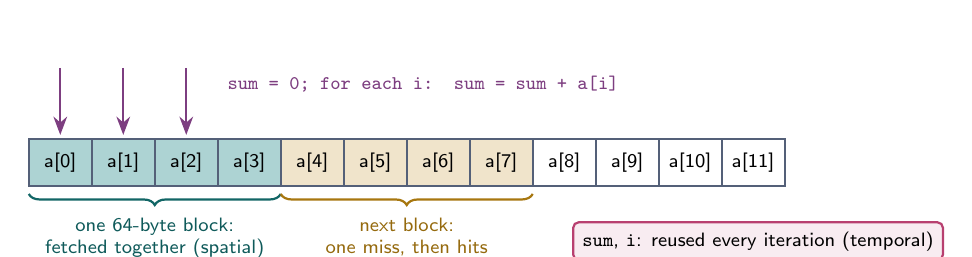
\begin{tikzpicture}[font=\sffamily\scriptsize]
  \foreach \i in {0,...,11} {
    \ifnum\i<4 \def\fc{tealC!35}\else\ifnum\i<8 \def\fc{amberC!22}\else\def\fc{white}\fi\fi
    \draw[thick, draw=slateC, fill=\fc] (\i*0.8,0) rectangle +(0.8,0.6);
    \node at (\i*0.8+0.4,0.3) {a[\i]};
  }
  \draw[decorate, decoration={brace, amplitude=4pt, mirror}, tealC!80!black, thick]
    (0,-0.1) -- (3.2,-0.1)
    node[midway, below=5pt, align=center, text=tealC!70!black]
    {one 64-byte block:\\fetched together (spatial)};
  \draw[decorate, decoration={brace, amplitude=4pt, mirror}, amberC!90!black, thick]
    (3.2,-0.1) -- (6.4,-0.1)
    node[midway, below=5pt, align=center, text=amberC!80!black]
    {next block:\\one miss, then hits};
  \draw[-{Stealth}, thick, plumC] (0.4,1.5) -- (0.4,0.65);
  \draw[-{Stealth}, thick, plumC] (1.2,1.5) -- (1.2,0.65);
  \draw[-{Stealth}, thick, plumC] (2.0,1.5) -- (2.0,0.65);
  \node[text=plumC, anchor=west] at (2.4,1.3)
       {\texttt{sum = 0; for each i: sum = sum + a[i]}};
  \node[draw, thick, rounded corners=2pt, fill=roseC!10, draw=roseC, anchor=west] at (6.9,-0.7)
       {\texttt{sum}, \texttt{i}: reused every iteration (temporal)};
\end{tikzpicture}
\end{bigfig}
\caption[Temporal and spatial locality]{Both kinds of locality in one loop.
Elements of \texttt{a} that share a block arrive together, so the miss on
\texttt{a[0]} brings \texttt{a[1]}--\texttt{a[3]} with it. The variables
\texttt{sum} and \texttt{i} are used on every iteration.}
\label{fig:locality}
\end{figure}

% ---------------------------------------------------------------
\section{How a Cache Is Organised}
\label{sec:cache-ops}
\label{sec:cache-mapping}
\sectionmap{[Organisation [Tag array + data array] [Address = tag | index | offset]
  [Set-associative: a few places per block]]}
\index{set-associative cache}\index{Sarangi textbook}%

A cache has two SRAM arrays side by side. The tag array records which memory block
each entry holds and the data array holds the bytes~\cite[\S11.2.2]{sarangi2025basic}.
The address is split into an offset (the byte within the block), an index (the
set to search) and a tag, which is compared with the stored tags to detect a hit.
A direct-mapped cache has one possible entry for each block. In a set-associative
cache\index{set-associative cache} the index picks a set of a few entries and all
of them are checked at once (\cref{fig:mapping}). Almost every real cache is set
associative.

Sarangi breaks the work of a cache into six operations: lookup, data read, data
write, insert, replace and evict~\cite[\S11.2.1]{sarangi2025basic}. On a miss the
cache fetches the block, picks a victim if the set is full (randomly, first-in
first-out or least recently used), evicts it and inserts the new
block~\cite[\S11.2.5]{sarangi2025basic}. A coherence protocol adds its own actions
to these same operations (Chapter~5).

\begin{figure}[htbp]
\centering
\begin{bigfig}
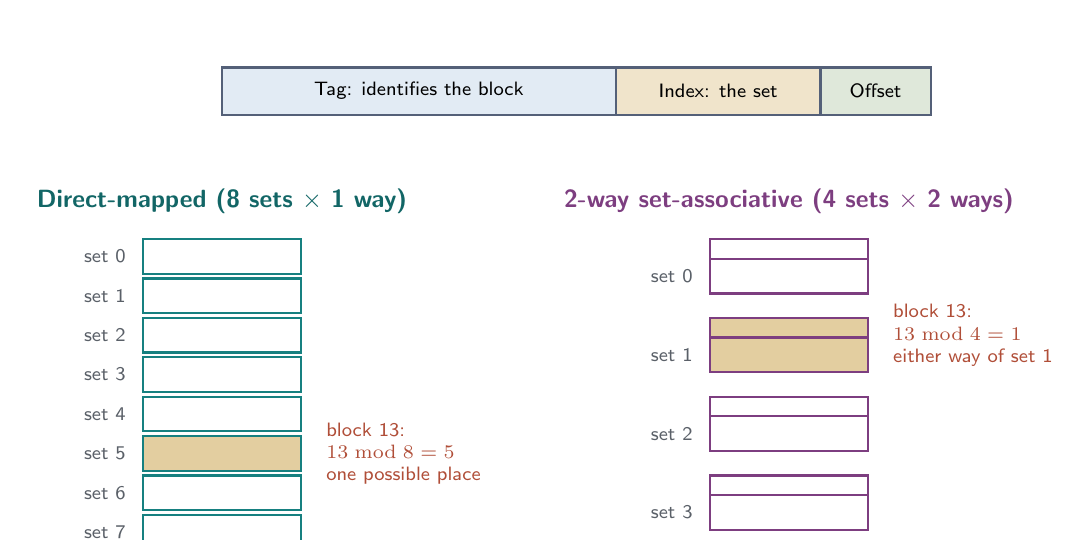
\begin{tikzpicture}[font=\sffamily\scriptsize]
  \begin{scope}[yshift=5.7cm, xshift=1.0cm]
  \draw[thick, draw=slateC, fill=skyC!14]   (0,0)   rectangle (5.0,0.6);
  \draw[thick, draw=slateC, fill=amberC!22] (5.0,0) rectangle (7.6,0.6);
  \draw[thick, draw=slateC, fill=leafC!18]  (7.6,0) rectangle (9.0,0.6);
  \node at (2.5,0.3) {Tag: identifies the block};
  \node at (6.3,0.3) {Index: the set};
  \node at (8.3,0.3) {Offset};
  \end{scope}
  \node[font=\sffamily\bfseries\small, text=tealC!80!black] at (1.0,4.6) {Direct-mapped (8 sets $\times$ 1 way)};
  \foreach \s in {0,...,7} {
    \pgfmathsetmacro{\y}{3.9-\s*0.5}
    \ifnum\s=5 \def\fc{amberC!40}\else\def\fc{white}\fi
    \node[anchor=east, text=coreGrey] at (-0.1,\y) {set \s};
    \draw[thick, draw=tealC, fill=\fc] (0,\y-0.22) rectangle (2.0,\y+0.22);
  }
  \node[text=brickC, align=left, anchor=west] at (2.2,1.4) {block 13:\\$13 \bmod 8 = 5$\\one possible place};
  \begin{scope}[xshift=7.2cm]
  \node[font=\sffamily\bfseries\small, text=plumC] at (1.0,4.6) {2-way set-associative (4 sets $\times$ 2 ways)};
  \foreach \s in {0,...,3} {
    \pgfmathsetmacro{\y}{3.9-\s*1.0}
    \ifnum\s=1 \def\fc{amberC!40}\else\def\fc{white}\fi
    \node[anchor=east, text=coreGrey] at (-0.1,\y-0.25) {set \s};
    \draw[thick, draw=plumC, fill=\fc] (0,\y-0.47) rectangle (2.0,\y-0.03);
    \draw[thick, draw=plumC, fill=\fc] (0,\y-0.03) rectangle (2.0,\y+0.22);
  }
  \node[text=brickC, align=left, anchor=west] at (2.2,2.9) {block 13:\\$13 \bmod 4 = 1$\\either way of set 1};
  \end{scope}
\end{tikzpicture}
\end{bigfig}
\caption[Address split and cache organisation]{Top: the address split used for
lookup. Bottom: eight entries arranged two ways. Block~13 has one possible entry
in the direct-mapped cache and two in the two-way cache, so it is evicted by
conflicts less often.}
\label{fig:mapping}
\end{figure}

% ---------------------------------------------------------------
\section{Writes, Misses and Dirty Victims}
\label{sec:cache-write}
\label{sec:cache-access}
\label{sec:cache-replacement}
\sectionmap{[Writes and misses [Write-through: update below every time]
  [Write-back: update only on eviction] [Dirty victim: write back first]]}
\index{MESI}\index{MOESI}\index{MSI}\index{write-back cache}\index{write-back cache!dirty bit}%

A read leaves the cache and memory in agreement, but a write does not, so the
cache must decide when to update the level below~\cite[\S11.2.3]{sarangi2025basic}.
A \gls{writethrough} sends every write down at once. The two levels then always
agree, but every store costs traffic. A \gls{writeback}\index{write-back cache}
updates only itself and sets a modified (dirty) bit, and the level below is
updated when the dirty block is evicted~\cite[\S11.2.6]{sarangi2025basic}. Since
programs write the same locations many times, almost every modern cache is write
back (\cref{fig:write-policies}).

\Cref{fig:access-tree} puts these steps into one decision tree. The branch at the
bottom left matters most for the rest of this report: evicting a modified block
costs a write to the level below, and evicting a clean block costs nothing. While
a block is dirty, the cache holds the only correct copy of its data and memory is
stale. The Modified state of MSI, MESI and MOESI (Chapter~5) is this dirty bit
extended to a system with many caches.

\begin{figure}[htbp]
\centering
\begin{minipage}[c]{0.46\linewidth}\centering
\adjustbox{max width=\linewidth}{%
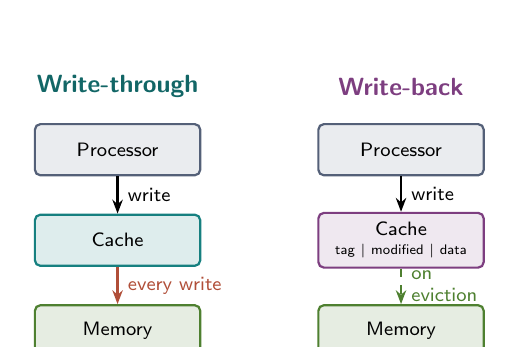
\begin{tikzpicture}[font=\sffamily\scriptsize,
    c/.style={draw, thick, rounded corners=2pt, minimum width=2.1cm,
              minimum height=0.65cm, align=center},
    a/.style={-{Stealth[length=5pt]}, thick}]
  \node[font=\sffamily\bfseries\small, text=tealC!80!black] at (1.1,3.3) {Write-through};
  \node[c, fill=slateC!12, draw=slateC] (p1) at (1.1,2.5) {Processor};
  \node[c, fill=tealC!14, draw=tealC] (c1) at (1.1,1.35) {Cache};
  \node[c, fill=leafC!14, draw=leafC] (m1) at (1.1,0.2) {Memory};
  \draw[a] (p1) -- node[right]{write} (c1);
  \draw[a, brickC] (c1) -- node[right]{every write} (m1);
  \begin{scope}[xshift=3.6cm]
  \node[font=\sffamily\bfseries\small, text=plumC] at (1.1,3.3) {Write-back};
  \node[c, fill=slateC!12, draw=slateC] (p2) at (1.1,2.5) {Processor};
  \node[c, fill=plumC!12, draw=plumC] (c2) at (1.1,1.35) {Cache\\[-1pt]\tiny tag $|$ modified $|$ data};
  \node[c, fill=leafC!14, draw=leafC] (m2) at (1.1,0.2) {Memory};
  \draw[a] (p2) -- node[right]{write} (c2);
  \draw[a, leafC, dashed] (c2) -- node[right, align=left]{on\\eviction} (m2);
  \end{scope}
\end{tikzpicture}}
\caption[Write-through and write-back caches]{The two write policies. A
write-back cache defers the memory update until eviction.}
\label{fig:write-policies}
\end{minipage}\hfill
\begin{minipage}[c]{0.5\linewidth}\centering
\adjustbox{max width=\linewidth}{%
\begin{forest}
  decision tree,
  [Tag matches in\\the indexed set?
    [Hit, el=yes
      [Return data, el=load]
      [Update data;\\set modified, el=store]]
    [Miss, el=no
      [Free entry?
        [Insert, el=yes]
        [Choose victim, el=no
          [Victim\\modified?
            [{Write back,\\then evict}, el=yes]
            [Evict\\silently, el=no]]]]]]
\end{forest}}
\caption[Decision tree: one cache access]{One access to a write-back cache. Only
a modified victim forces a write to the level below.}
\label{fig:access-tree}
\end{minipage}
\end{figure}

% ---------------------------------------------------------------
\section{The Memory Hierarchy, AMAT and the Three Cs}
\label{sec:cache-hierarchy}
\label{sec:cache-3c}
\sectionmap{[Hierarchy [L1 small and fast] [{L2, L3 larger and slower}]
  [AMAT measures the whole] [Three kinds of miss]]}
\index{AMAT}\index{Sarangi textbook}%

Processors stack several levels of cache, each larger and slower than the one
above it (\cref{fig:hierarchy})~\cite[\S11.1.7]{sarangi2025basic}. The usual
figure of merit is the \gls{amat}\index{AMAT}. For two levels of
cache~\cite[\S11.3.1]{sarangi2025basic},
\begin{equation}
  \mathrm{AMAT} = T_{L1} + m_{L1}\bigl(T_{L2} + m_{L2}\,T_{\mathrm{mem}}\bigr),
  \label{eq:amat}
\end{equation}
where $T$ is the latency of each level and $m$ its local miss rate. With
$T_{L1}=1$, $T_{L2}=10$ and $T_{\mathrm{mem}}=100$ cycles and both miss rates at
10\,\%, AMAT is 3 cycles, compared with 100 cycles without caches. This is the
33$\times$ improvement of Sarangi's Example~147.

\begin{figure}[htbp]
\centering
\begin{bigfig}[0.85]
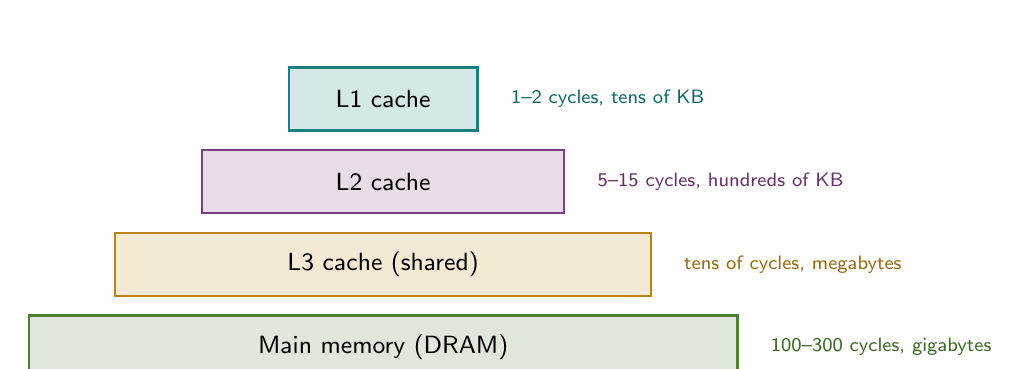
\begin{tikzpicture}[font=\sffamily\small]
  \def\layer#1#2#3#4#5{
    \draw[thick, fill=#5!18, draw=#5] (-#2/2,#1) rectangle (#2/2,#1+0.8);
    \node at (0,#1+0.4) {#3};
    \node[font=\sffamily\scriptsize, text=#5!80!black, anchor=west] at (#2/2+0.3,#1+0.4) {#4};
  }
  \layer{0}{9.0}{Main memory (DRAM)}{100--300 cycles, gigabytes}{leafC}
  \layer{1.05}{6.8}{L3 cache (shared)}{tens of cycles, megabytes}{amberC}
  \layer{2.1}{4.6}{L2 cache}{5--15 cycles, hundreds of KB}{plumC}
  \layer{3.15}{2.4}{L1 cache}{1--2 cycles, tens of KB}{tealC}
\end{tikzpicture}
\end{bigfig}
\caption[The memory hierarchy]{Each level is larger and slower than the one
above. L1, L2 and memory latencies follow Sarangi~\cite[\S11.1.7]{sarangi2025basic};
the L3 figures are indicative.}
\label{fig:hierarchy}
\end{figure}

Misses are traditionally put into three classes~\cite[\S11.3.2]{sarangi2025basic}
(\cref{tab:three-c}). All three describe a single core and its own cache. A
fourth class, which appears only when cores share data, comes up in Part~II.

\begin{table}[htbp]
\centering
\caption{The three classic kinds of cache miss.}
\label{tab:three-c}
\small
\begin{tabular}{@{}l p{5.4cm} p{4.0cm}@{}}
\toprule
Kind & Cause & Typical remedy \\
\midrule
Compulsory (cold) & first access to a block & larger blocks, prefetching \\
Capacity & working set larger than the cache & larger cache \\
Conflict & too many blocks map to one set & higher associativity \\
\bottomrule
\end{tabular}
\end{table}

% ---------------------------------------------------------------
\section{Private and Shared Caches}
\label{sec:cache-private}
\sectionmap{[Private vs shared [{Shared: one copy, many ports}]
  [Private: small and close to the core] [Result: many copies of one block]]}

On a multicore chip the cores can share one cache or each have their own
(\cref{fig:private-shared}). A shared cache keeps one copy of each block but has
to serve every core at once. The area of a cache grows roughly with the square of
its number of ports, and a large shared array cannot sit close to every
core~\cite[\S12.4.4]{sarangi2025basic}. Private caches are small and sit next to
their core. Modern chips therefore give each core a private L1 (and usually L2)
and share only the \gls{llc}.

\begin{figure}[htbp]
\centering
\begin{bigfig}[0.9]
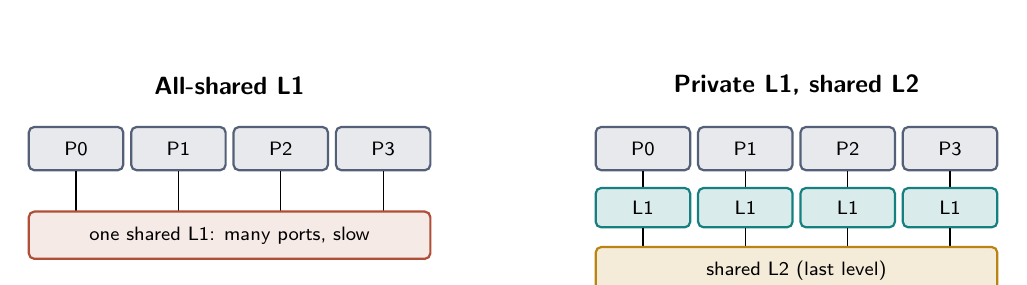
\begin{tikzpicture}[font=\sffamily\scriptsize,
    core/.style={draw, thick, rounded corners=2pt, fill=slateC!14, draw=slateC,
                 minimum width=1.2cm, minimum height=0.55cm},
    pc/.style={draw, thick, rounded corners=2pt, fill=tealC!16, draw=tealC,
               minimum width=1.2cm, minimum height=0.5cm},
    sc/.style={draw, thick, rounded corners=2pt, fill=amberC!16, draw=amberC,
               minimum height=0.6cm}]
  \node[font=\sffamily\bfseries\small] at (1.95,2.6) {All-shared L1};
  \foreach \i in {0,1,2,3} { \node[core] (a\i) at (\i*1.3,1.8) {P\i}; \draw (a\i) -- (\i*1.3,1.0); }
  \node[sc, minimum width=5.1cm, fill=brickC!12, draw=brickC] at (1.95,0.7) {one shared L1: many ports, slow};
  \begin{scope}[xshift=7.2cm]
  \node[font=\sffamily\bfseries\small] at (1.95,2.6) {Private L1, shared L2};
  \foreach \i in {0,1,2,3} {
    \node[core] (b\i) at (\i*1.3,1.8) {P\i};
    \node[pc] (l\i) at (\i*1.3,1.05) {L1};
    \draw (b\i) -- (l\i); \draw (l\i) -- (\i*1.3,0.55);
  }
  \node[sc, minimum width=5.1cm] at (1.95,0.25) {shared L2 (last level)};
  \end{scope}
\end{tikzpicture}
\end{bigfig}
\caption[Shared and private caches]{Two ways to organise the caches of a
four-core chip. Real designs use private L1 caches for speed, and as a result one
block can be copied into several of them.}
\label{fig:private-shared}
\end{figure}

This report assumes the right-hand design throughout. It is fast, and it lets
the same memory block sit in several private caches at the same time. Chapter~3
explains why many cores run one program over a shared memory, and Chapter~4
explains how the private copies are kept consistent.

% ===============================================================
%  Chapter 3 -- Parallel Processing and Multicore Systems   (Part I)
% ===============================================================
\chapter{Parallel Processing and Multicore Systems}
\label{ch:parallel}

\begin{figure}[htbp]
\centering
\adjustbox{max width=\linewidth}{%
\begin{forest}
  chapter map,
  [Chapter 3
    [From one core to many [Frequency wall] [MIMD multicores]]
    [Shared memory {\&} threads [Fork--join in OpenMP]]
    [Interconnects [{Bus, ring, mesh}]]
    [Amdahl's law [Speedup ceiling] [Why coherence is needed]]
  ]
\end{forest}}
\caption[]{Structure of Chapter~3: why chips became
multicore, how they are programmed and connected, what limits the gain from more
cores, and where coherence becomes necessary.}
\label{fig:ch3-map}
\end{figure}

% ---------------------------------------------------------------
\section{From One Core to Many}
\label{sec:par-why}
\label{sec:par-defs}
\label{sec:par-flynn}
\sectionmap{[One core is not enough [Clock speed stalled near 3 GHz]
  [Little more parallelism in one program] [Spend transistors on more cores]]}
\index{Sarangi textbook}%

Until the mid-2000s an unchanged program ran faster on each new processor. Then
clock frequency levelled off at around 3\,GHz, because beyond that point power and
heat grew faster than performance, and wide superscalar cores could no longer find
enough independent instructions to issue~\cite[\S12.1]{sarangi2025basic}. Moore's
law~\cite{moore1965cramming} still gave designers more transistors each
generation, so they spent them on several simpler cores in place of one bigger
core.

Sarangi defines \emph{multiprocessing} as several processors working in parallel,
and a \emph{multicore processor}\index{multicore processor} as a multiprocessor
whose processors (cores) share one chip~\cite[\S12.1, Def.~116]{sarangi2025basic}.
In Flynn's taxonomy~\cite{flynn1972organizations}\cite[\S12.3]{sarangi2025basic} a
multicore is a MIMD machine, since every core fetches its own instructions and
works on its own operands. Multiprocessors came first. By the late 1990s
motherboards carried four or eight processors, IBM's POWER4 put two cores on one
chip in 2001, and Intel and AMD followed in 2005~\cite[\S12.1]{sarangi2025basic}.
This report deals with the multicore case, where the cores share one chip and one
physical address space.

% ---------------------------------------------------------------
\section{Shared Memory, Threads and Fork--Join}
\label{sec:par-sm-mp}
\label{sec:par-threads}
\sectionmap{[Programming model [Shared memory: common load and store]
  [Message passing: explicit send] [Fork--join threads share data]]}
\index{Sarangi textbook}%

Parallel programs communicate in one of two ways (\cref{fig:sm-mp}). Threads in a
shared-memory program use one address space and exchange data with ordinary loads
and stores. Processes in a message-passing program, such as one written with MPI,
have private memories and exchange data only through explicit \texttt{send} and
\texttt{receive} calls~\cite[\S12.2.2]{sarangi2025basic}. Coherence is needed only
in the shared-memory case, because only there can two cores cache the same
location.

\begin{figure}[htbp]
\centering
\begin{bigfig}[0.85]
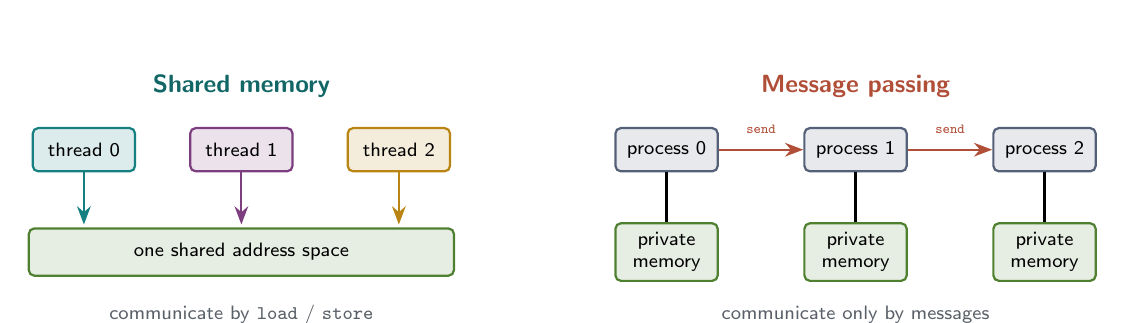
\begin{tikzpicture}[font=\sffamily\scriptsize,
    u/.style={draw, thick, rounded corners=2pt, minimum width=1.3cm, minimum height=0.55cm},
    m/.style={draw, thick, rounded corners=2pt, fill=leafC!14, draw=leafC,
              minimum height=0.6cm, align=center}]
  \node[font=\sffamily\bfseries\small, text=tealC!80!black] at (2.0,2.7) {Shared memory};
  \foreach \i/\c in {0/tealC,1/plumC,2/amberC} { \node[u, fill=\c!15, draw=\c] (t\i) at (\i*2.0,1.9) {thread \i}; \draw[thick, -{Stealth}, \c] (t\i) -- (\i*2.0,0.95); }
  \node[m, minimum width=5.4cm] at (2.0,0.6) {one shared address space};
  \node[text=coreGrey] at (2.0,-0.2) {communicate by \texttt{load} / \texttt{store}};
  \begin{scope}[xshift=7.4cm]
  \node[font=\sffamily\bfseries\small, text=brickC] at (2.4,2.7) {Message passing};
  \foreach \i in {0,1,2} {
    \node[u, fill=slateC!14, draw=slateC] (p\i) at (\i*2.4,1.9) {process \i};
    \node[m, minimum width=1.3cm] (mm\i) at (\i*2.4,0.6) {private\\memory};
    \draw[thick] (p\i) -- (mm\i);
  }
  \draw[-{Stealth}, thick, brickC] (p0) -- node[above=2pt, font=\sffamily\tiny]{\texttt{send}} (p1);
  \draw[-{Stealth}, thick, brickC] (p1) -- node[above=2pt, font=\sffamily\tiny]{\texttt{send}} (p2);
  \node[text=coreGrey] at (2.4,-0.2) {communicate only by messages};
  \end{scope}
\end{tikzpicture}
\end{bigfig}
\caption[Shared memory and message passing]{The two programming models. Only the
left-hand model has locations that two cores can both cache.}
\label{fig:sm-mp}
\end{figure}

Sarangi defines a thread as a sub-program with its own program counter and stack
that runs in the same address space as other threads of the
program~\cite[\S12.2.2, Def.~120]{sarangi2025basic}. Shared-memory programs usually
follow the fork--join pattern. A sequential section starts $N$ threads, each thread
works on its slice of the data, the program waits for all of them, and then it
combines their results. \Cref{lst:omp} shows this in \gls{openmp}.

\begin{lstlisting}[language=C, caption={Fork--join in OpenMP: summing an array in parallel.}, label=lst:omp]
double partial[NTHREADS];               /* shared array of results  */
#pragma omp parallel num_threads(NTHREADS)
{
    int me = omp_get_thread_num();      /* which slice is mine?     */
    int first = me * (N / NTHREADS), last = first + N / NTHREADS;
    double s = 0;
    for (int k = first; k < last; k++) s += a[k];
    partial[me] = s;                    /* write a shared location  */
}                                       /* implicit join here       */
double sum = 0;
for (int t = 0; t < NTHREADS; t++) sum += partial[t];
\end{lstlisting}

The statement \texttt{partial[me] = s} writes a shared array that another core
reads after the join. The program says nothing about how the value travels to the
reading core, so the hardware has to handle it.

% ---------------------------------------------------------------
\section{Interconnection Networks}
\label{sec:par-noc}
\sectionmap{[Interconnects [Bus: one shared medium] [Ring and mesh: point-to-point]
  [Diameter and bisection bandwidth]]}
\index{network on chip}%

Cores and caches exchange messages over an on-chip interconnect, or
\gls{noc}\index{network on chip}. Two numbers describe it. The diameter is the
longest shortest path between two nodes, which sets the worst-case latency. The
bisection bandwidth is the smallest number of links that must be cut to split the
network in half, which limits throughput~\cite[\S12.6.2]{sarangi2025basic}.
\Cref{fig:topologies,tab:topologies} compare the topologies used in multicores.

\begin{figure}[htbp]
\centering
\begin{minipage}[c]{0.66\linewidth}\centering
\adjustbox{max width=\linewidth}{%
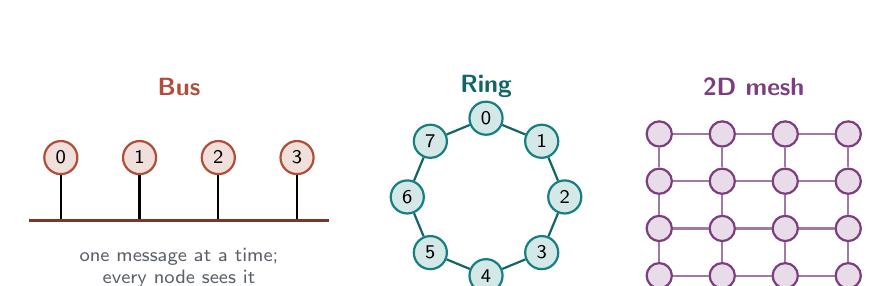
\begin{tikzpicture}[font=\sffamily\scriptsize,
    n/.style={circle, thick, minimum size=0.42cm, inner sep=0pt}]
  \node[font=\sffamily\bfseries\small, text=brickC] at (1.5,2.9) {Bus};
  \foreach \i in {0,...,3} { \node[n, draw=brickC, fill=brickC!18] (b\i) at (\i*1.0,2.0) {\i}; \draw[thick] (b\i) -- (\i*1.0,1.2); }
  \draw[very thick, brickC!70!black] (-0.4,1.2) -- (3.4,1.2);
  \node[text=coreGrey, align=center] at (1.5,0.6) {one message at a time;\\every node sees it};
  \begin{scope}[xshift=5.4cm, yshift=1.5cm]
  \node[font=\sffamily\bfseries\small, text=tealC!80!black] at (0,1.4) {Ring};
  \foreach \i in {0,...,7} { \node[n, draw=tealC, fill=tealC!18] (r\i) at ({90-\i*45}:1.0) {\i}; }
  \foreach \i [evaluate=\i as \j using {int(mod(\i+1,8))}] in {0,...,7} { \draw[thick, tealC!80!black] (r\i) -- (r\j); }
  \end{scope}
  \begin{scope}[xshift=7.6cm, yshift=0.5cm]
  \node[font=\sffamily\bfseries\small, text=plumC] at (1.2,2.4) {2D mesh};
  \foreach \x in {0,...,3} \foreach \y in {0,...,3} {
    \node[n, minimum size=0.32cm, draw=plumC, fill=plumC!18] (m\x\y) at (\x*0.8,\y*0.6) {};
  }
  \foreach \x in {0,...,3} \foreach \y [count=\yy] in {0,...,2} { \draw[thick, plumC!70] (m\x\y) -- (m\x\yy); }
  \foreach \y in {0,...,3} \foreach \x [count=\xx] in {0,...,2} { \draw[thick, plumC!70] (m\x\y) -- (m\xx\y); }
  \end{scope}
\end{tikzpicture}}
\captionof{figure}[Three interconnect topologies]{A bus, an eight-node ring and a
$4\times4$ mesh. A bus delivers each message to every node; rings and meshes
carry point-to-point messages and scale further.}
\label{fig:topologies}
\end{minipage}\hfill
\begin{minipage}[c]{0.31\linewidth}\centering\small
\captionof{table}{Diameter and bisection bandwidth for $N$ nodes~\cite[\S12.6.3]{sarangi2025basic}.}
\label{tab:topologies}
\setlength{\tabcolsep}{3pt}
\begin{tabular}{@{}lcc@{}}
\toprule
 & Diam. & Bisect. \\
\midrule
Ring & $N/2$ & 2 \\
Mesh & $2\sqrt{N}-2$ & $\sqrt{N}$ \\
Torus & $\approx\sqrt{N}$ & $2\sqrt{N}$ \\
Fat tree & $2\log N$ & $N/2$ \\
\bottomrule
\end{tabular}
\end{minipage}
\end{figure}

A bus has a property the other topologies do not get for free. Only one message
is on it at a time, so every node sees every message in the same order.
Chapter~4 uses this property.

% ---------------------------------------------------------------
\section{Amdahl's Law and the Need for Coherence}
\label{sec:par-amdahl}
\label{sec:par-coherence}
\sectionmap{[Amdahl's law [Parallel fraction f] [Speedup saturates at 1/(1-f)]
  [Private caches + shared memory = coherence]]}
\index{Amdahl's law}%

If a fraction $f$ of the work spreads perfectly over $p$ cores and the rest runs on
one core, the speedup is~\cite{amdahl1967validity}\cite[\S12.2.3]{sarangi2025basic}
\begin{equation}
  S(p) = \frac{1}{(1-f) + f/p},
  \label{eq:amdahl}
\end{equation}
which tends to $1/(1-f)$ as $p$ grows (\cref{fig:amdahl}). A system close to this
ceiling can behave quite differently from the same system with two cores, which is
why our experiments sweep 2, 4, 8 and 16 cores.

\begin{figure}[htbp]
\centering
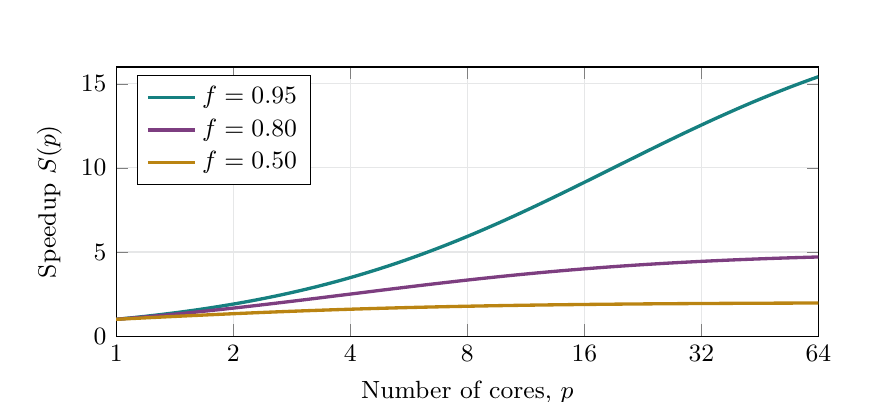
\begin{tikzpicture}
  \begin{axis}[width=10.5cm, height=5cm,
      xlabel={Number of cores, $p$}, ylabel={Speedup $S(p)$},
      xmin=1, xmax=64, ymin=0, ymax=16,
      xtick={1,2,4,8,16,32,64}, xticklabels={1,2,4,8,16,32,64},
      xmode=log, log basis x=2,
      legend pos=north west, legend style={font=\small},
      grid=major, grid style={coreGrey!15},
      label style={font=\small}, tick label style={font=\small}]
    \addplot[very thick, tealC, domain=1:64, samples=100] {1/((1-0.95)+0.95/x)};
    \addlegendentry{$f=0.95$}
    \addplot[very thick, plumC, domain=1:64, samples=100] {1/((1-0.80)+0.80/x)};
    \addlegendentry{$f=0.80$}
    \addplot[very thick, amberC, domain=1:64, samples=100] {1/((1-0.50)+0.50/x)};
    \addlegendentry{$f=0.50$}
  \end{axis}
\end{tikzpicture}
\caption[Amdahl's law]{\Cref{eq:amdahl} for three parallel fractions. With
95\,\% of the program parallel, speedup can never pass $1/(1-f)=20$, and at 16
cores it is well below that.}
\label{fig:amdahl}
\end{figure}

Chapters~2 and~3 have now made two design choices. Each core has a private cache
so that the first level stays fast (\cref{sec:cache-private}), and all cores share
one address space so that programs like \cref{lst:omp} are easy to write. Together
they allow one memory block to sit in several private caches at once, so the
system needs a rule for keeping the copies consistent (coherence) and hardware
that enforces the rule on every access (a coherence protocol). Chapter~4 covers
both.

% ===============================================================
%  Chapter 4 -- How Cache Coherence Is Maintained        (Part I)
% ===============================================================
\chapter{How Cache Coherence Is Maintained}
\label{ch:coherence-basics}

\begin{figure}[htbp]
\centering
\adjustbox{max width=\linewidth}{%
\begin{forest}
  chapter map,
  [Chapter 4
    [What coherence means [Completion {\&} order axioms] [Not consistency]]
    [Block states [Event / action]]
    [Snooping and directories [Bus orders messages] [Sharer list]]
    [Update vs invalidate [Decision tree]]
  ]
\end{forest}}
\caption[]{Structure of Chapter~4: what a coherence
protocol must guarantee, then the parts every protocol is built from.}
\label{fig:ch4-map}
\end{figure}

% ---------------------------------------------------------------
\section{What Coherence Means}
\label{sec:coh-meaning}
\label{sec:coh-order}
\label{sec:coh-consistency}
\sectionmap{[Coherence [Concerns one address] [Completion: no write is lost]
  [Order: one order for all threads] [{Consistency: a separate question}]]}
\index{coherence axioms}\index{memory consistency}\index{Sarangi textbook}%

To a program, a set of private caches has to look like one cache. Sarangi states
the requirement in terms of the accesses to a single
address~\cite[\S12.4.2, Def.~122]{sarangi2025basic}\index{coherence axioms}:

\begin{keybox}[The two axioms of coherence]
\emph{Completion}: a write must eventually complete, and the memory system may
never lose it.\\[3pt]
\emph{Order}: all threads see the writes to one address in the same order.
\end{keybox}

However many copies of a location the machine holds, it must behave like a single
location whose value changes in one agreed sequence. \Cref{fig:order-example}
draws Sarangi's example of the order axiom~\cite[\S12.4.2, Ex.~151]{sarangi2025basic}.
Thread~1 writes \texttt{x=1} and then \texttt{x=2}, and thread~2 reads \texttt{x}
twice. Every pair of results can occur except $(2,1)$, which would mean thread~2
saw the second write before the first. A coherence protocol is the hardware that
enforces both axioms for every block in every cache.

Coherence says nothing about writes to different addresses. Whether another
thread may see a new value of \texttt{y} together with an old value of \texttt{x}
after thread~1 wrote \texttt{x} and then \texttt{y} is a question of memory
consistency~\cite[\S12.4.3]{sarangi2025basic}. We keep the consistency model fixed
and study coherence only.

% ---------------------------------------------------------------
\section{Block States and State Machines}
\label{sec:coh-fsm}
\sectionmap{[States [Each cached block has a state] [Events cause transitions]
  [Written as event / action]]}

All the protocols in this report work the same way. Every block in every cache
has a small state stored next to its tag, and the cache controller runs a finite
state machine for each block. When an event arrives, the controller performs an
action and may move the block to a new state~\cite[\S12.4.6]{sarangi2025basic}.
Events come either from the cache's own processor (read, write, evict) or from
other caches through the interconnect (\cref{fig:fsm-notation}). A block that is
not in the cache counts as Invalid.

\begin{figure}[htbp]
\centering
\begin{minipage}[c]{0.5\linewidth}\centering
\adjustbox{max width=\linewidth}{%
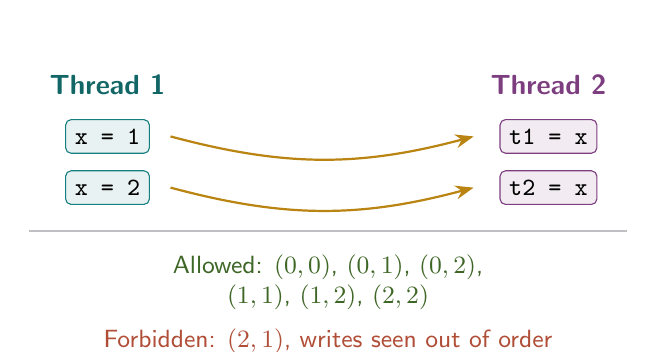
\begin{tikzpicture}[font=\sffamily\small]
  \node[font=\sffamily\bfseries, text=tealC!80!black] at (0,2.0) {Thread 1};
  \node[font=\sffamily\bfseries, text=plumC] at (5.6,2.0) {Thread 2};
  \node[draw=tealC, fill=tealC!10, rounded corners=2pt] at (0,1.35) {\texttt{x = 1}};
  \node[draw=tealC, fill=tealC!10, rounded corners=2pt] at (0,0.7) {\texttt{x = 2}};
  \node[draw=plumC, fill=plumC!10, rounded corners=2pt] at (5.6,1.35) {\texttt{t1 = x}};
  \node[draw=plumC, fill=plumC!10, rounded corners=2pt] at (5.6,0.7) {\texttt{t2 = x}};
  \draw[-{Stealth}, thick, amberC] (0.8,1.35) to[out=-15,in=195] (4.65,1.35);
  \draw[-{Stealth}, thick, amberC] (0.8,0.7) to[out=-15,in=195] (4.65,0.7);
  \draw[thick, coreGrey!40] (-1.0,0.15) -- (6.6,0.15);
  \node[text=leafC!80!black, align=center] at (2.8,-0.5) {Allowed: $(0,0)$, $(0,1)$, $(0,2)$,\\$(1,1)$, $(1,2)$, $(2,2)$};
  \node[text=brickC] at (2.8,-1.25) {Forbidden: $(2,1)$, writes seen out of order};
\end{tikzpicture}}
\caption[The order axiom]{The order axiom: only $(2,1)$ is impossible.}
\label{fig:order-example}
\end{minipage}\hfill
\begin{minipage}[c]{0.45\linewidth}\centering
\adjustbox{max width=\linewidth}{%
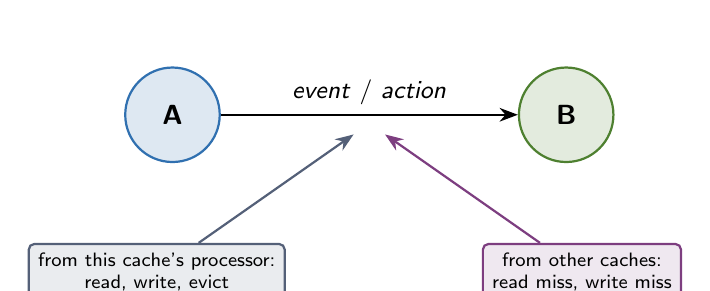
\begin{tikzpicture}[font=\sffamily\small, >=Stealth,
    st/.style={draw, thick, circle, minimum size=1.2cm, font=\sffamily\bfseries}]
  \node[st, fill=skyC!16, draw=skyC] (A) at (0,0) {A};
  \node[st, fill=leafC!16, draw=leafC] (B) at (5,0) {B};
  \draw[->, thick] (A) -- node[above]{\textit{event} / \textit{action}} (B);
  \node[draw, thick, rounded corners=2pt, fill=slateC!12, draw=slateC, align=center, font=\sffamily\scriptsize]
       (p) at (-0.2,-2.0) {from this cache's processor:\\read, write, evict};
  \node[draw, thick, rounded corners=2pt, fill=plumC!12, draw=plumC, align=center, font=\sffamily\scriptsize]
       (o) at (5.2,-2.0) {from other caches:\\read miss, write miss};
  \draw[->, thick, slateC] (p) -- (2.3,-0.25);
  \draw[->, thick, plumC] (o) -- (2.7,-0.25);
\end{tikzpicture}}
\caption[State-machine notation]{Notation for every protocol in this report.}
\label{fig:fsm-notation}
\end{minipage}
\end{figure}

% ---------------------------------------------------------------
\section{Snooping and Directory Protocols}
\label{sec:coh-snoop}
\label{sec:coh-dir}
\sectionmap{[Organisation [Snooping: every cache watches the bus]
  [Bus order gives the order axiom] [Directory: sharer list per block]]}
\index{snooping protocol}\index{directory protocol}\index{coherence axioms}%

In a \gls{snoop}\index{snooping protocol} all private caches sit on one shared bus.
One cache puts a message on the bus at a time and every other cache reads
it~\cite[\S12.4.6]{sarangi2025basic}. Each controller watches (snoops) the bus and
reacts to messages about blocks it holds. An arbiter grants the bus to requesters
in FIFO order~\cite[\S13.4.3]{sarangi2025basic} (\cref{fig:snoop-bus}). Since only
one cache transmits at a time, all caches see all messages in the same order, and
the order axiom holds automatically~\cite[\S12.4.6]{sarangi2025basic}. One
consequence is easy to miss. A cache that wants to write must wait for its own
request to appear on the bus before updating its copy. If it wrote first, two
caches writing at the same moment could each apply their own write first and see
the two writes in opposite orders~\cite[\S12.4.6, Question~8]{sarangi2025basic}.

\begin{figure}[htbp]
\centering
\begin{minipage}[c]{0.55\linewidth}\centering
\adjustbox{max width=\linewidth}{%
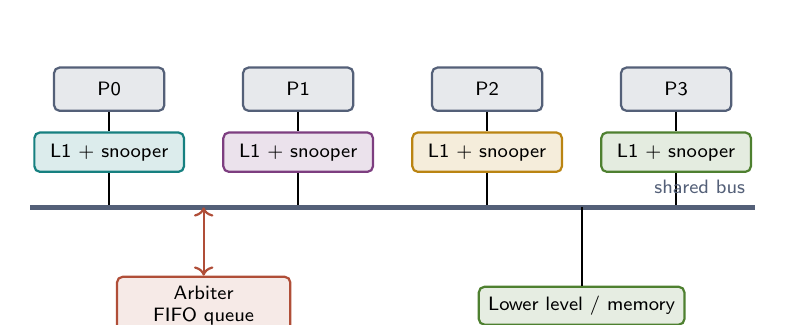
\begin{tikzpicture}[font=\sffamily\scriptsize,
    cpu/.style={draw, thick, rounded corners=2pt, fill=slateC!14, draw=slateC,
                minimum width=1.4cm, minimum height=0.55cm},
    cache/.style={draw, thick, rounded corners=2pt, minimum width=1.9cm,
                  minimum height=0.5cm}]
  \foreach \i/\c in {0/tealC,1/plumC,2/amberC,3/leafC} {
    \node[cpu] (c\i) at (\i*2.4,2.3) {P\i};
    \node[cache, fill=\c!15, draw=\c] (h\i) at (\i*2.4,1.5) {L1 + snooper};
    \draw[thick] (c\i) -- (h\i); \draw[thick] (h\i) -- (\i*2.4,0.8);
  }
  \draw[line width=2pt, slateC] (-1.0,0.8) -- (8.2,0.8);
  \node[text=slateC, anchor=south east] at (8.2,0.85) {shared bus};
  \node[draw, thick, rounded corners=2pt, fill=brickC!12, draw=brickC,
        minimum width=2.2cm, align=center] (arb) at (1.2,-0.45) {Arbiter\\FIFO queue};
  \draw[thick, brickC, <->] (arb) -- (1.2,0.8);
  \node[draw, thick, rounded corners=2pt, fill=leafC!14, draw=leafC,
        minimum width=2.4cm] (mem) at (6.0,-0.45) {Lower level / memory};
  \draw[thick] (mem) -- (6.0,0.8);
\end{tikzpicture}}
\caption[A snooping system]{Four private caches on a shared bus. The arbiter
lets one cache transmit at a time.}
\label{fig:snoop-bus}
\end{minipage}\hfill
\begin{minipage}[c]{0.42\linewidth}\centering
\adjustbox{max width=\linewidth}{%
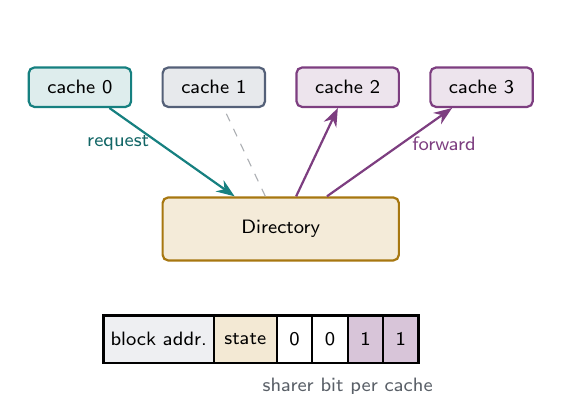
\begin{tikzpicture}[font=\sffamily\scriptsize,
    cache/.style={draw, thick, rounded corners=2pt, minimum width=1.3cm, minimum height=0.5cm}]
  \foreach \i/\c in {0/tealC,1/slateC,2/plumC,3/plumC} { \node[cache, fill=\c!14, draw=\c] (h\i) at (\i*1.7,2.2) {cache \i}; }
  \node[draw, thick, rounded corners=2pt, fill=amberC!16, draw=amberC!90!black,
        minimum width=3.0cm, minimum height=0.8cm] (d) at (2.55,0.4) {Directory};
  \draw[-{Stealth}, thick, tealC] (h0) -- node[left, pos=0.4, text=tealC!80!black]{request} (d);
  \draw[-{Stealth}, thick, plumC] (d) -- (h2);
  \draw[-{Stealth}, thick, plumC] (d) -- node[right, pos=0.6, text=plumC]{forward} (h3);
  \draw[dashed, coreGrey!50] (d) -- (h1);
  \begin{scope}[xshift=0.3cm, yshift=-1.3cm]
    \draw[thick, fill=slateC!10] (0,0) rectangle (1.4,0.6); \node at (0.7,0.3) {block addr.};
    \draw[thick, fill=amberC!18] (1.4,0) rectangle (2.2,0.6); \node at (1.8,0.3) {state};
    \foreach \b/\v in {0/0,1/0,2/1,3/1} {
      \ifnum\v=1 \def\fc{plumC!30}\else\def\fc{white}\fi
      \draw[thick, fill=\fc] (2.2+\b*0.45,0) rectangle +(0.45,0.6);
      \node at (2.425+\b*0.45,0.3) {\v};
    }
    \node[text=coreGrey] at (3.1,-0.3) {sharer bit per cache};
  \end{scope}
\end{tikzpicture}}
\caption[A directory protocol]{The directory forwards cache~0's request only to
the recorded sharers, caches~2 and~3.}
\label{fig:directory}
\end{minipage}
\end{figure}

Broadcasting every request wastes bandwidth when only one or two caches hold the
block. A \gls{directory}\index{directory protocol} keeps a record for each block of
the caches that may hold a copy, usually one bit per
cache~\cite[\S12.4.6]{sarangi2025basic}. Requests go to the directory, which
forwards them only to the caches concerned (\cref{fig:directory}). Censier and
Feautrier proposed the scheme in 1978~\cite{censier1978directory}.
\Cref{tab:snoop-dir} sums up the trade-off.

\begin{table}[htbp]
\centering
\caption{Snooping and directory organisations compared.}
\label{tab:snoop-dir}
\small
\begin{tabular}{@{}l p{4.8cm} p{4.8cm}@{}}
\toprule
 & Snooping & Directory \\
\midrule
Who sees a request & every cache & only the recorded sharers \\
Ordering of messages & provided by the bus & enforced by the directory \\
Extra storage & none & a directory entry per block \\
Interconnect & shared bus & any (ring, mesh, \ldots) \\
Scales to & a small number of cores & many cores \\
\bottomrule
\end{tabular}
\end{table}

% ---------------------------------------------------------------
\section{Write-Update and Write-Invalidate}
\label{sec:coh-update-invalidate}
\label{sec:coh-choose}
\sectionmap{[Two strategies [Update: send new value to all copies]
  [Invalidate: destroy other copies] [MSI family is write-invalidate]]}
\index{MSI}\index{snooping protocol}\index{directory protocol}\index{write-update}\index{write-invalidate}\index{Dragon protocol}\index{Firefly protocol}\index{Sarangi textbook}%

A protocol must also decide what happens to the other copies when one cache writes
a block~\cite[\S12.4.6]{sarangi2025basic}. Under \gls{update}\index{write-update}
the writer sends each new value out and every other copy is updated in place, so
each write to shared data costs a message. Under
\gls{invalidate}\index{write-invalidate} the writer first removes every other
copy, after which it can write as often as it likes without further messages. At
any moment a block then has either one writer or any number of readers. Sarangi
justifies write-invalidate by noting that most blocks are not shared at the moment
they are written. This choice is separate from the snooping-or-directory choice.
The MSI family of Chapter~5 is write-invalidate and exists in both snooping and
directory forms, while Dragon and Firefly (Part~III) are snooping write-update
protocols. \Cref{fig:choose-tree} puts both choices into one decision tree. Real
designs mix them, for example by snooping within a cluster and using a directory
between clusters. From here on every protocol is write-invalidate unless stated
otherwise.

\begin{figure}[htbp]
\centering
\adjustbox{max width=0.8\linewidth}{%
\begin{forest}
  decision tree,
  [Few cores sharing\\one bus?
    [Snooping, el=yes
      [Same core usually\\rewrites before\\others read?
        [{Snooping +\\invalidate\\(MSI family)}, el=yes]
        [{Snooping +\\update}, el=no]]]
    [Directory, el=no
      [Same core usually\\rewrites before\\others read?
        [{Directory +\\invalidate}, el=yes]
        [{Directory +\\update}, el=no]]]]
\end{forest}}
\caption[Decision tree: choosing a coherence organisation]{The two design
questions of this chapter. Real programs usually answer the second question
``yes'', which is why write-invalidate is the common choice.}
\label{fig:choose-tree}
\end{figure}

% ===============================================================
%  Chapter 5 -- The MSI Family: MSI, MESI and MOESI      (Part I)
% ===============================================================
\chapter{The MSI Family: MSI, MESI and MOESI}
\label{ch:msi-family}
\index{MESI}\index{MOESI}\index{MSI}%

\begin{figure}[htbp]
\centering
\adjustbox{max width=\linewidth}{%
\begin{forest}
  chapter map,
  [Chapter 5
    [Events {\&} messages [Processor events] [Bus messages]]
    [MSI [Three states] [Two state diagrams]]
    [MESI [Adds Exclusive] [Silent upgrade]]
    [MOESI [Adds Owned] [Read-miss decision tree]]
    [A worked trace [Same accesses in all three] [The family at a glance]]
  ]
\end{forest}}
\caption[]{Structure of Chapter~5. Each protocol is given
in the same order (states, transitions on processor events, transitions on
messages from other caches) so the three can be compared line by line.}
\label{fig:ch5-map}
\end{figure}

This chapter describes what each of the three protocols does. Which one costs
less is the subject of Parts~II and~III.

% ---------------------------------------------------------------
\section{Events and Messages}
\label{sec:fam-events}
\sectionmap{[Vocabulary [Processor events: read write evict]
  [Bus messages: readmiss writemiss write] [Responses: data and write back]
  [Hits change nothing]]}
\index{write-invalidate}\index{Sarangi textbook}%

The three protocols react to the same events and use the message names of
Sarangi's write-invalidate protocol~\cite[\S12.4.6]{sarangi2025basic}
(\cref{tab:events}). Read hits in any valid state and write hits in \stM\ change
no state and send no message, so the diagrams leave them out.

\begin{table}[htbp]
\centering
\caption{Events and messages used by the MSI family.}
\label{tab:events}
\small
\begin{tabular}{@{}l l p{7.6cm}@{}}
\toprule
Kind & Name & Meaning \\
\midrule
Processor event & read / write & the local core loads or stores the block \\
 & evict & the local cache removes the block to make room \\
\midrule
Bus message & \textit{readmiss} & another cache wants to read a block it does not hold \\
 & \textit{writemiss} & another cache wants to write a block it does not hold \\
 & \textit{write} & another cache holds the block and is about to write it
   (an upgrade); other copies must be invalidated \\
\midrule
Response & \textit{send data} & a cache supplies the block to the requester \\
 & \textit{write back} & a cache writes the block to the lower level \\
\bottomrule
\end{tabular}
\end{table}

% ---------------------------------------------------------------
\section{MSI: Three States}
\label{sec:fam-msi}
\sectionmap{[MSI [M: only copy and modified] [S: read-only and clean]
  [I: not present] [One writer or many readers]]}
\index{MSI}\index{write-invalidate}\index{Sarangi textbook}%

The basic write-invalidate protocol, \gls{msi}\index{MSI}, has three states per
block~\cite[\S12.4.6]{sarangi2025basic}:

\begin{description}
  \item[\stM\ (Modified).] This cache may write the block. No other cache
    holds a valid copy. The data differs from memory.
  \item[\stS\ (Shared).] This cache may read but not write the block. Other
    caches may hold \stS\ copies too. The data matches memory.
  \item[\stI\ (Invalid).] The cache holds no valid copy.
\end{description}

\Cref{fig:msi} redraws Sarangi's two diagrams: transitions caused by the local
processor (his Fig.~12.13) and transitions caused by messages from other caches
(his Fig.~12.14). The red transition in part~(b) comes up again and again in this
report. When another cache reads a block held in \stM, this cache sends the data,
writes the block back to the lower level, and moves to \stS.

\tikzset{
  fsm/.style={font=\sffamily\small, >=Stealth, node distance=2cm},
  st/.style={draw, thick, circle, minimum size=1.05cm, font=\sffamily\bfseries},
  stB/.style={st, fill=mesiBlue!14, draw=mesiBlue},
  stO/.style={st, fill=moesiOrange!14, draw=moesiOrange},
  stT/.style={st, fill=tealC!16, draw=tealC},
  tr/.style={->, thick, slateC},
  bus/.style={->, thick, dashed, plumC},
  key/.style={->, very thick, alertRed},
  good/.style={->, very thick, memGreen},
  lb/.style={font=\sffamily\tiny, fill=white, inner sep=1pt, align=center},
}

\begin{figure}[htbp]
\centering
\begin{bigfig}
\begin{tikzpicture}[fsm]
  \node[font=\sffamily\bfseries\small] at (2.4,4.2) {(a) Processor events};
  \node[stT] (I) at (0,0) {\stI};
  \node[stT] (S) at (4.8,0) {\stS};
  \node[stT] (M) at (2.4,3.0) {\stM};
  \draw[tr] (I) to[bend right=18] node[lb, below]{read / readmiss} (S);
  \draw[tr] (S) to[bend right=18] node[lb, above]{evict / ---} (I);
  \draw[tr] (I) to[bend left=12] node[lb, left=2pt]{write /\\writemiss} (M);
  \draw[tr] (M) to[bend left=12] node[lb, right=1pt]{evict /\\write back} (I);
  \draw[tr] (S) -- node[lb, right=3pt]{write /\\write} (M);
  \begin{scope}[xshift=7.4cm]
  \node[font=\sffamily\bfseries\small] at (2.4,4.2) {(b) Messages from other caches};
  \node[stT] (I2) at (0,0) {\stI};
  \node[stT] (S2) at (4.8,0) {\stS};
  \node[stT] (M2) at (2.4,3.0) {\stM};
  \draw[bus] (S2) -- node[lb, below]{write, writemiss / ---} (I2);
  \draw[bus] (M2) -- node[lb, left=2pt]{writemiss /\\send data} (I2);
  \draw[key] (M2) -- node[lb, right=3pt, text=alertRed]{readmiss /\\send data\\+ \textbf{write back}} (S2);
  \end{scope}
\end{tikzpicture}
\end{bigfig}
\caption[MSI state diagrams]{The MSI protocol, redrawn from Sarangi's
Figs.~12.13 and~12.14~\cite[\S12.4.6]{sarangi2025basic}. Solid arrows are caused
by the local processor and dashed purple arrows by messages from other caches. The
red transition writes the block back when another cache reads it.}
\label{fig:msi}
\end{figure}

% ---------------------------------------------------------------
\section{MESI: Adding an Exclusive State}
\label{sec:fam-mesi}
\sectionmap{[MESI [Read of unshared data enters E] [E is clean and the only copy]
  [E to M needs no message] [Origin: Illinois protocol 1984]]}
\index{MESI}\index{MSI}\index{Exclusive state}\index{Illinois protocol}\index{Sarangi textbook}%

When a core reads a block that no other cache holds, such as its own stack
data, MSI still puts the block in \stS\ because it cannot tell that this is the
only copy. When the core then writes the block, the cache has to send a
\textit{write} message to invalidate copies that do not exist.
\Gls{mesi}\index{MESI} adds a fourth state for this case~\cite{papamarcos1984illinois}:

\begin{description}
  \item[\stE\ (Exclusive).] No other cache has a copy and the data matches
    memory. The cache may read the block and may move it to \stM\ on a write
    without sending any message, since no other cache needs to know.
\end{description}

On a read miss the other caches report whether any of them holds the block, for
example by asserting a ``shared'' line on the bus. If none does, the block enters
\stE\ instead of \stS. Sarangi introduces this state and leaves ``implementing
the MESI protocol\,\ldots as an exercise for the
reader''~\cite[\S12.4.6, p.~603]{sarangi2025basic}; \cref{fig:mesi} is our
solution.

\begin{figure}[htbp]
\centering
\adjustbox{max width=\linewidth}{%
\begin{tikzpicture}[fsm]
  \node[font=\sffamily\bfseries\small] at (2.9,4.1) {(a) Processor events};
  \node[stB] (I) at (0,1.5) {\stI};
  \node[stB] (E) at (2.9,3.2) {\stE};
  \node[stB] (S) at (2.9,-0.2) {\stS};
  \node[stB] (M) at (5.8,1.5) {\stM};
  \draw[tr] (I) -- node[lb, above left=-1pt]{read, no copies /\\readmiss} (E);
  \draw[tr] (I) -- node[lb, below left=-1pt]{read, copies exist /\\readmiss} (S);
  \draw[tr] (I) to[bend left=9] node[lb, above, pos=0.62]{write / writemiss} (M);
  \draw[tr] (M) to[bend left=9] node[lb, below, pos=0.62]{evict / write back} (I);
  \draw[good] (E) -- node[lb, above right=-1pt, text=memGreen]{write / ---\\\textbf{(silent)}} (M);
  \draw[tr] (S) -- node[lb, below right=-1pt]{write / write} (M);
  \node[lb, text=coreGrey, anchor=west] at (-0.4,-1.0) {Evict from \stE\ or \stS: silent, to \stI.};
  \begin{scope}[xshift=7.7cm, yshift=0.4cm]
  \node[font=\sffamily\bfseries\small] at (2.8,3.8) {(b) Messages from other caches};
  \node[stB] (E2) at (0,2.4) {\stE};
  \node[stB] (S2) at (2.8,2.4) {\stS};
  \node[stB] (M2) at (5.6,2.4) {\stM};
  \node[stB] (I2) at (2.8,-0.4) {\stI};
  \draw[bus] (E2) -- node[lb, above=3pt]{readmiss /\\send data} (S2);
  \draw[key] (M2) -- node[lb, above=3pt, text=alertRed]{readmiss / send data\\+ \textbf{write back}} (S2);
  \draw[bus] (E2) -- node[lb, left=2pt, pos=0.45]{writemiss /\\send data} (I2);
  \draw[bus] (S2) -- node[lb, pos=0.45]{write,\\writemiss / ---} (I2);
  \draw[bus] (M2) -- node[lb, right=2pt, pos=0.45]{writemiss /\\send data} (I2);
  \end{scope}
\end{tikzpicture}}
\caption[MESI state diagrams]{The MESI protocol. The green transition is what
MESI adds: a block in \stE\ moves to \stM\ silently. The red transition is the
same as in MSI, so a remote read of an \stM\ block still causes a write back.}
\label{fig:mesi}
\end{figure}

% ---------------------------------------------------------------
\section{MOESI: Adding an Owned State}
\label{sec:fam-moesi}
\label{sec:fam-readmiss}
\sectionmap{[MOESI [O: modified but shared] [Owner supplies data]
  [Owner is responsible for write back] [Origin: Futurebus 1986]]}
\index{MESI}\index{MOESI}\index{Owned state}\index{snooping protocol}\index{Futurebus}\index{owner}%

\Gls{moesi}\index{MOESI} adds a fifth state to MESI~\cite{sweazey1986moesi}:

\begin{description}
  \item[\stO\ (Owned).] The copy is modified, so memory is stale, but other
    caches may hold the same data in \stS. The owning cache answers every request
    for the block and must write it back to memory when it evicts it.
\end{description}

The only change from MESI is the red transition of \cref{fig:mesi}. In MOESI, when
another cache reads a block held in \stM, the holder sends the data and moves to
\stO\ without writing back (\cref{fig:moesi}). An \stS\ copy may then differ from
memory, because the latest data is in the \gls{owner}\index{owner}, and the owner
must write the block back when it evicts it, as an \stM\ block must.
\Cref{fig:readmiss-tree} shows how a snooping system serves a read miss under both
protocols. They agree on every branch except the last.

\begin{figure}[htbp]
\centering
\adjustbox{max width=\linewidth}{%
\begin{forest}
  decision tree,
  [Read miss: does another\\cache hold the block?
    [Requester enters E\\data from memory, el=no]
    [Is that copy\\in M or O?, el=yes
      [Requester enters S\\any E copy drops to S, el=no]
      [Which protocol?, el=yes
        [MESI: owner sends data\\writes back and enters S, el=MESI]
        [MOESI: owner sends data\\enters or stays in O\\no write back, el=MOESI]]]]
\end{forest}}
\caption[Decision tree: serving a read miss]{How a read miss is served in MESI
and MOESI. The protocols differ only in the bottom row, where a cache holding
modified data is read by another cache.}
\label{fig:readmiss-tree}
\end{figure}


\begin{figure}[htbp]
\centering
\begin{bigfig}
\begin{tikzpicture}[fsm]
  \node[font=\sffamily\bfseries\small, anchor=west] at (-0.5,3.2) {(a) Processor events: the two transitions new in MOESI};
  \node[stO] (M) at (1.9,2.0) {\stM};
  \node[stO] (O) at (3.8,0) {\stO};
  \node[stO] (I) at (0,0) {\stI};
  \draw[tr] (O) -- node[lb, right=2pt]{write /\\write} (M);
  \draw[tr] (O) -- node[lb, below]{evict / write back} (I);
  \node[lb, text=coreGrey, align=left, anchor=west] at (5.0,1.0)
       {All other processor-side transitions are\\exactly as in MESI (\cref{fig:mesi}a).};
  \begin{scope}[yshift=-5.6cm]
  \node[font=\sffamily\bfseries\small, anchor=west] at (-0.5,3.9) {(b) Messages from other caches};
  \node[stO] (E2) at (0,2.4) {\stE};
  \node[stO] (S2) at (3.0,2.4) {\stS};
  \node[stO] (M2) at (6.0,2.4) {\stM};
  \node[stO] (O2) at (9.0,2.4) {\stO};
  \node[stO] (I2) at (4.5,-0.6) {\stI};
  \draw[bus] (E2) -- node[lb, above=3pt]{readmiss /\\send data} (S2);
  \draw[good] (M2) -- node[lb, above=3pt, text=memGreen]{readmiss / send data\\\textbf{no write back}} (O2);
  \draw[bus] (O2) to[loop right, looseness=5] node[lb, right]{readmiss /\\send data} (O2);
  \draw[bus] (E2) -- node[lb, left=3pt, pos=0.5]{writemiss / send data} (I2);
  \draw[bus] (S2) -- node[lb, pos=0.45]{write,\\writemiss / ---} (I2);
  \draw[bus] (M2) -- node[lb, pos=0.45]{writemiss /\\send data} (I2);
  \draw[bus] (O2) -- node[lb, right=3pt, pos=0.5]{write, writemiss / send data if asked} (I2);
  \end{scope}
\end{tikzpicture}
\end{bigfig}
\caption[MOESI state diagrams]{The MOESI protocol. Part~(a) shows only the two
processor-side transitions that MOESI adds. In part~(b) the green transition
replaces MESI's red one: the cache with modified data supplies it and moves to
\stO\ without writing back, and then answers every later read miss itself (the
loop on \stO).}
\label{fig:moesi}
\end{figure}

Some combinations of states in different caches would break coherence, so each
protocol allows only certain pairs for the same block. \Cref{tab:compat} gives the
rule for MOESI. The one new pair is $(\stO,\stS)$, which is modified data that is
also shared.

\begin{table}[htbp]
\centering
\caption{Which states two caches may hold for the same block at the same time
in MOESI ($\checkmark$ = allowed). Removing the \stO\ row and column gives the
rule for MESI.}
\label{tab:compat}
\small
\begin{tabular}{@{}c|ccccc@{}}
 & \stM & \stO & \stE & \stS & \stI \\
\hline
\stM & $\times$ & $\times$ & $\times$ & $\times$ & \checkmark \\
\stO & $\times$ & $\times$ & $\times$ & \checkmark & \checkmark \\
\stE & $\times$ & $\times$ & $\times$ & $\times$ & \checkmark \\
\stS & $\times$ & \checkmark & $\times$ & \checkmark & \checkmark \\
\stI & \checkmark & \checkmark & \checkmark & \checkmark & \checkmark \\
\end{tabular}
\end{table}

% ---------------------------------------------------------------
\section{A Worked Trace}
\label{sec:fam-trace}
\sectionmap{[Worked trace [Three cores and one block] [Six accesses]
  [States in MSI MESI MOESI] [E appears at step 1] [O appears at step 3]]}
\index{MESI}\index{MOESI}\index{MSI}\index{Owned state}\index{Exclusive state}\index{owner}%

\Cref{tab:trace} follows one block through six accesses by three cores under
each protocol. The block starts in no cache.

\begin{table}[htbp]
\centering
\caption{One block, six accesses, three protocols. Cells give the states in
P0 / P1 / P2 after each step.}
\label{tab:trace}
\small
\begin{tabular}{@{}c l c c c@{}}
\toprule
Step & Access & MSI & MESI & MOESI \\
\midrule
1 & P0 reads  & S / I / I & \textbf{E} / I / I & \textbf{E} / I / I \\
2 & P0 writes & M / I / I & M / I / I & M / I / I \\
3 & P1 reads  & S / S / I & S / S / I & \textbf{O} / S / I \\
4 & P2 reads  & S / S / S & S / S / S & \textbf{O} / S / S \\
5 & P1 writes & I / M / I & I / M / I & I / M / I \\
6 & P0 reads  & S / S / I & S / S / I & S / \textbf{O} / I \\
\bottomrule
\end{tabular}
\end{table}

At step~1 MESI and MOESI put the block in \stE, since no other cache holds it;
MSI has no such state. At step~2 the move to \stM\ is silent in MESI and MOESI
and costs a bus \textit{write} in MSI. At steps~3, 4 and~6 MOESI keeps the
modified data in an owner (\stO), while MSI and MESI fall back to all-\stS. At
step~5 ownership passes to the new writer, and P0's \stO\ copy is invalidated
because P1's write makes it out of date.

\label{sec:fam-glance}
\Cref{tab:family} describes every state of the family by four properties and
shows which protocol uses it.

\begin{table}[htbp]
\centering
\caption{Every state of the MSI family.}
\label{tab:family}
\small
\begin{tabular}{@{}c c c c c c c c@{}}
\toprule
State & Valid & Differs from & Only & Responsible for & \multicolumn{3}{c}{Used in} \\
\cmidrule(l){6-8}
 & & memory & copy & write back & MSI & MESI & MOESI \\
\midrule
\stM & yes & yes & yes & yes & \checkmark & \checkmark & \checkmark \\
\stO & yes & yes & no  & yes &            &            & \checkmark \\
\stE & yes & no  & yes & no  &            & \checkmark & \checkmark \\
\stS & yes & no$^{*}$ & no & no & \checkmark & \checkmark & \checkmark \\
\stI & no  & --- & --- & no  & \checkmark & \checkmark & \checkmark \\
\midrule
\multicolumn{5}{@{}l}{Bits of state per block} & 2 & 2 & 3 \\
\bottomrule
\multicolumn{8}{@{}l}{\footnotesize $^{*}$ In MOESI, an \stS\ copy may differ
from memory when another cache holds the block in \stO.}
\end{tabular}
\end{table}

MESI is therefore MSI with the clean, unshared case taken out of \stS\ and given
its own state \stE, and MOESI is MESI with a dirty, shared case added as \stO.

% ===============================================================
%  Chapter 6 -- A History of the Protocols               (Part I)
% ===============================================================
\chapter{A History of the Protocols}
\label{ch:history}

\begin{figure}[htbp]
\centering
\adjustbox{max width=\linewidth}{%
\begin{forest}
  chapter map,
  [Chapter 6
    [First schemes [Directory 1978] [Write-once 1983]]
    [Snooping in the 1980s [Illinois {\&} Berkeley] [MOESI vocabulary 1986]]
    [Beyond the bus [{DASH, tokens}] [{AMD MOESI, Intel MESIF}]]
  ]
\end{forest}}
\caption[]{Structure of Chapter~6: the protocols of
Chapter~5 in the order they appeared.}
\label{fig:ch6-map}
\end{figure}

The protocols of Chapter~5 grew out of work on bus-based multiprocessors in the
1980s, long before multicore chips. \Cref{fig:timeline} shows the milestones that
matter for this report, and Part~III returns to several of them.

\begin{figure}[htbp]
\centering
\begin{bigfig}
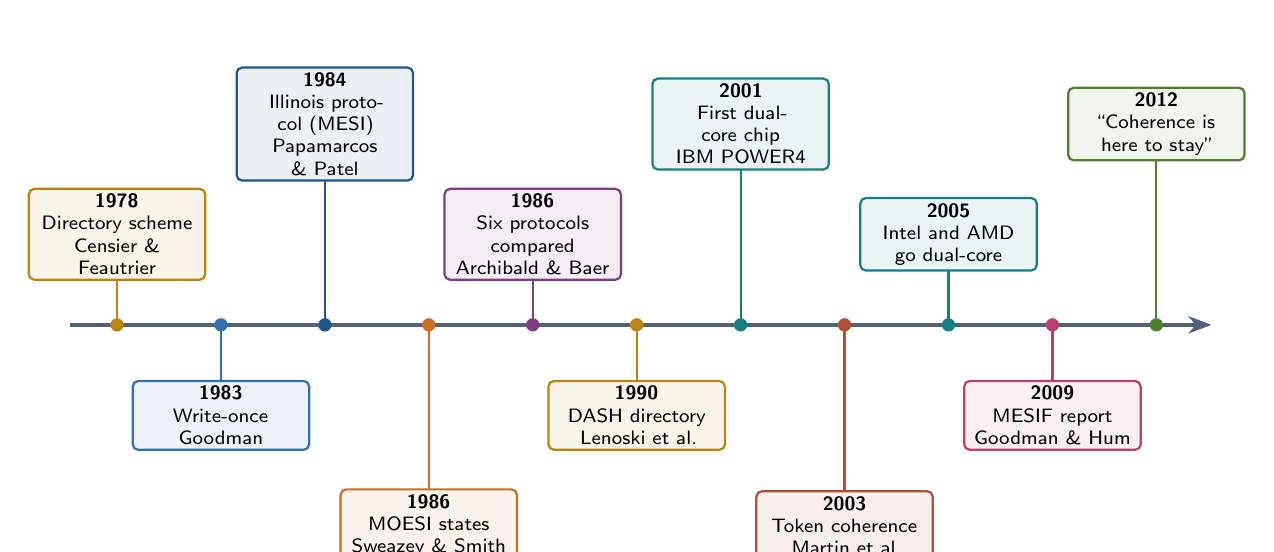
\begin{tikzpicture}[font=\sffamily\scriptsize,
    ev/.style={draw, thick, rounded corners=2pt, align=center, inner sep=2pt,
               text width=2.1cm}]
  \draw[very thick, slateC, -{Stealth}] (-0.6,0) -- (13.9,0);
  \foreach \i/\y/\lev/\txt/\col in {
      0/1978/1.15/{Directory scheme\\Censier {\&} Feautrier}/amberC,
      1/1983/-1.15/{Write-once\\Goodman}/skyC,
      2/1984/2.55/{Illinois protocol (MESI)\\Papamarcos {\&} Patel}/mesiBlue,
      3/1986/-2.55/{MOESI states\\Sweazey {\&} Smith}/moesiOrange,
      4/1986/1.15/{Six protocols compared\\Archibald {\&} Baer}/plumC,
      5/1990/-1.15/{DASH directory\\Lenoski et al.}/amberC,
      6/2001/2.55/{First dual-core chip\\IBM POWER4}/tealC,
      7/2003/-2.55/{Token coherence\\Martin et al.}/brickC,
      8/2005/1.15/{Intel and AMD\\go dual-core}/tealC,
      9/2009/-1.15/{MESIF report\\Goodman {\&} Hum}/roseC,
      10/2012/2.55/{``Coherence is\\here to stay''}/leafC} {
    \pgfmathsetmacro{\x}{\i*1.32}
    \pgfmathsetmacro{\e}{\lev>0 ? \lev-0.42 : \lev+0.42}
    \draw[\col, thick] (\x,0) -- (\x,\e);
    \fill[\col] (\x,0) circle (2.4pt);
    \node[ev, draw=\col, fill=\col!9] at (\x,\lev) {\textbf{\y}\\\txt};
  }
\end{tikzpicture}
\end{bigfig}
\caption[Timeline of coherence protocols]{Milestones from the first directory
scheme to current multicore chips, in date order but not to scale. Sources are
cited in the text.}
\label{fig:timeline}
\end{figure}

% ---------------------------------------------------------------
\section{The First Coherence Schemes}
\label{sec:hist-before}
\label{sec:hist-first}
\sectionmap{[First schemes [Several processors on one bus] [1978: a central directory]
  [1983: write-once on a bus]]}
\index{snooping protocol}\index{directory protocol}%

Multiprocessors go back to the 1960s and 1970s, and by the late 1990s four or
eight processors commonly shared one motherboard and one
bus~\cite[\S12.1]{sarangi2025basic}. As soon as processors with private caches
shared a bus, coherence became an engineering problem. The first general scheme
was a directory. Censier and Feautrier proposed in 1978 that memory keep, for each
block, a record of the caches holding it, so that invalidations went only where
they were needed~\cite{censier1978directory}. The first widely known snooping
protocol was Goodman's write-once~\cite{goodman1983writeonce}, with the states
Invalid, Valid, Reserved and Dirty~\cite{archibald1986evaluation}. The first write
to a block went through to memory and invalidated the other copies, and later
writes stayed in the cache. Every later protocol keeps the main idea of
write-once, which is to use the bus both for moving data and for telling other
caches what has happened to it.

% ---------------------------------------------------------------
\section{Snooping Protocols of the 1980s and the MOESI Vocabulary}
\label{sec:hist-1980s}
\label{sec:hist-moesi}
\sectionmap{[1980s snooping [Illinois: the E state] [Berkeley: a shared-dirty owner]
  [Firefly and Dragon: update] [1986: five states describe them all]]}
\index{MESI}\index{MOESI}\index{MSI}\index{MESIF}\index{Owned state}\index{Exclusive state}\index{snooping protocol}\index{write-update}\index{Berkeley protocol}\index{Dragon protocol}\index{Firefly protocol}\index{Illinois protocol}\index{Futurebus}\index{owner}%

In 1986 Archibald and Baer described and simulated six snooping protocols side by
side~\cite{archibald1986evaluation}. \Cref{tab:hist-protocols} translates their
state names into the terms of Chapter~5. Two of them matter most here. The
Illinois protocol of Papamarcos and Patel added a Valid-Exclusive state so that a
later write needed no bus transaction~\cite{papamarcos1984illinois}, which is
MESI. The Berkeley protocol had a Shared-Dirty state in which one cache kept
modified data, other caches held copies, and the Shared-Dirty cache supplied the
data to readers~\cite{archibald1986evaluation}. That is the \stO\ state before it
had the name. Firefly and Dragon were write-update protocols.

\begin{table}[htbp]
\centering
\caption{The six protocols evaluated by Archibald and
Baer~\cite{archibald1986evaluation}, with each original state name mapped to
its nearest MOESI equivalent.}
\label{tab:hist-protocols}
\small
\begin{tabular}{@{}l l l l@{}}
\toprule
Protocol & Original states & In MOESI terms & Strategy \\
\midrule
Write-once & Invalid, Valid, Reserved, Dirty & I, S, E, M & invalidate \\
Synapse    & Invalid, Valid, Dirty & I, S, M & invalidate \\
Illinois   & Invalid, Valid-Exclusive, Shared, Dirty & I, E, S, M & invalidate \\
Berkeley   & Invalid, Valid, Shared-Dirty, Dirty & I, S, \textbf{O}, M & invalidate \\
Firefly    & Valid-Exclusive, Shared, Dirty & E, S, M & update \\
Dragon     & Valid-Exclusive, Shared-Clean, Shared-Dirty, Dirty & E, S, \textbf{O}, M & update \\
\bottomrule
\end{tabular}
\end{table}

By the mid-1980s these protocols used different names for overlapping ideas.
While working on the IEEE Futurebus standard, Sweazey and Smith picked out five
states (Modified, Owned, Exclusive, Shared and Invalid) that could describe a
whole class of protocols, and showed how protocols of that class could share one
bus~\cite{sweazey1986moesi}. MOESI began as a shared vocabulary for existing
protocols more than as one new design. MESI and the ownership idea each add one
state to MSI, MOESI combines the two, and MESIF (Part~III) extends MESI in another
direction.

% ---------------------------------------------------------------
\section{Beyond the Bus and onto the Chip}
\label{sec:hist-scaling}
\label{sec:hist-multicore}
\sectionmap{[Recent history [1990: DASH directory] [2003: token coherence]
  [AMD: MOESI; Intel: MESIF]]}
\index{MOESI}\index{MSI}\index{MESIF}\index{directory protocol}\index{token coherence}\index{DASH}%

A bus carries one message at a time, which limits the number of processors it can
serve. The Stanford DASH machine of 1990 kept MSI-family states but replaced the
bus with a directory and a network of point-to-point links~\cite{lenoski1990dash}.
In 2003 Martin, Hill and Wood proposed token coherence~\cite{martin2003token}.
Both come back in Part~III. When the cores moved onto one chip in the
2000s~\cite[\S12.1]{sarangi2025basic}, AMD documented a MOESI
protocol~\cite{amd64vol2} and Intel's QuickPath processors adopted
MESIF~\cite{goodman2009mesif}. In 2012 Martin, Hill and Sorin argued that hardware
coherence will stay practical as core counts grow~\cite{martin2012here}. AMD and
Intel have kept different extensions of the same protocol for years, and Part~II
asks what each extension costs.


% ---------------------------------------------------------------
\part{The Problem: Unnecessary Memory Writebacks When Caches Share Modified Data}
\label{part:problem}
% ===============================================================
%  Part II overview -- sits directly under the Part II heading
% ===============================================================
\begin{center}
\adjustbox{max width=\linewidth}{%
\begin{forest}
  part map,
  [Part II
    [Ch.~7: Where the Cost Comes From
      [Stale copies] [Messages] [Coherence misses]]
    [Ch.~8: How the Cost Grows
      [Broadcast] [Bus saturation] [Coherence in AMAT]]
    [Ch.~9: Forced Writebacks
      [The transaction] [Root cause] [Sharing patterns]]
    [Ch.~10: Problem Statement
      [Formal statement] [Research questions]]
  ]
\end{forest}}
\end{center}

\begin{keybox}[What Part II does]
Part~II looks at what coherence costs. Chapter~7 traces the cost to its origin,
Chapter~8 shows how it grows as cores are added, and Chapter~9 isolates the one
inefficiency this report studies: the writeback MESI performs whenever another
cache reads a modified block. Chapter~10 states the problem formally and poses
the research questions. Remedies, including MOESI, are judged only in Part~III.
\end{keybox}

% ===============================================================
%  Chapter 7 -- Where the Cost of Coherence Comes From   (Part II)
% ===============================================================
\chapter{Where the Cost of Coherence Comes From}
\label{ch:origin}

\begin{figure}[htbp]
\centering
\adjustbox{max width=\linewidth}{%
\begin{forest}
  chapter map,
  [Chapter 7
    [The stale copy [Two caches disagree] [Hardware must fix it]]
    [Every action is a message [{Control, data, write back}] [Six-step MESI bill]]
    [A fourth kind of miss [Coherence misses]]
  ]
\end{forest}}
\caption[]{Structure of Chapter~7: from the failure
coherence prevents to an itemised bill for preventing it.}
\label{fig:ch7-map}
\end{figure}

% ---------------------------------------------------------------
\section{The Stale Copy, and Why Hardware Must Prevent It}
\label{sec:orig-stale}
\label{sec:orig-hardware}
\sectionmap{[Stale copy [Core 0 writes into its own cache] [Core 1 reads memory]
  [Gets an old value] [Hardware must prevent it on every access]]}
\index{write-back cache}%

\Cref{fig:stale} shows what goes wrong without coherence, using only private
write-back caches (\cref{sec:cache-write}) and a shared address space
(\cref{sec:par-sm-mp}). Core~0 writes \texttt{x=1}. The new value stays in core~0's
write-back cache and memory still holds \texttt{0}. Core~1 then reads \texttt{x},
misses and fetches the block from memory, so it gets \texttt{0}, a value that has
already been overwritten. Each component did its job, yet the program reads the
wrong value.

\begin{figure}[htbp]
\centering
\begin{bigfig}[0.85]
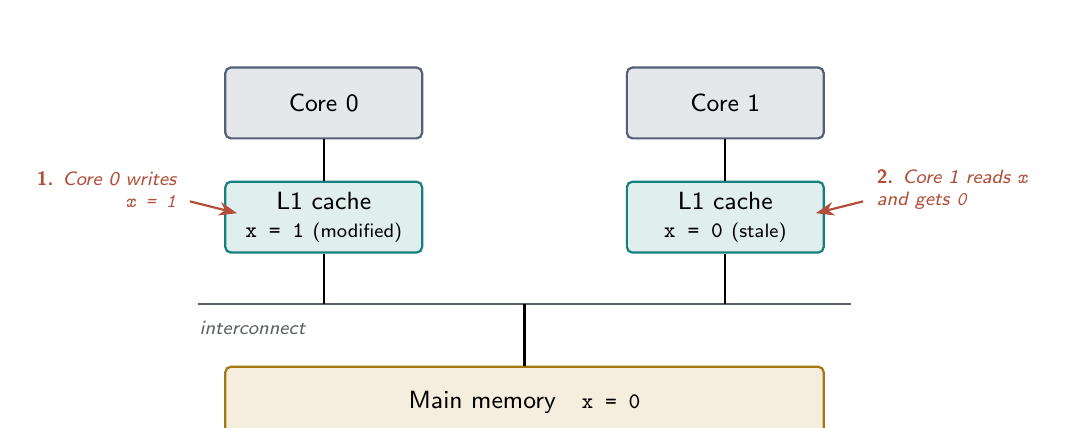
\begin{tikzpicture}[font=\sffamily\small,
    box/.style={draw, rounded corners=2pt, minimum width=2.5cm,
                minimum height=0.9cm, align=center, thick},
    core/.style={box, fill=slateC!15, draw=slateC},
    cache/.style={box, fill=tealC!13, draw=tealC},
    mem/.style={box, fill=amberC!14, draw=amberC!90!black, minimum width=7.6cm},
    lbl/.style={font=\sffamily\scriptsize\itshape, text=brickC}]
  \node[core] (c0) at (0,3.5) {Core 0};
  \node[core] (c1) at (5.1,3.5) {Core 1};
  \node[cache] (l0) at (0,2.05) {L1 cache\\[-1pt]{\footnotesize\ttfamily x = 1}\ {\scriptsize(modified)}};
  \node[cache] (l1) at (5.1,2.05) {L1 cache\\[-1pt]{\footnotesize\ttfamily x = 0}\ {\scriptsize(stale)}};
  \draw[thick, coreGrey] (-1.6,0.95) -- (6.7,0.95);
  \node[font=\sffamily\scriptsize\itshape, text=coreGrey, anchor=west] at (-1.7,0.65) {interconnect};
  \node[mem] (mm) at (2.55,-0.3) {Main memory\quad{\footnotesize\ttfamily x = 0}};
  \draw[thick] (c0) -- (l0); \draw[thick] (c1) -- (l1);
  \draw[thick] (l0) -- (0,0.95); \draw[thick] (l1) -- (5.1,0.95);
  \draw[thick] (2.55,0.95) -- (mm);
  \node[lbl, anchor=east, align=right] at (-1.75,2.4) {\textbf{1.} Core 0 writes\\\texttt{x = 1}};
  \node[lbl, anchor=west, align=left] at (6.9,2.4) {\textbf{2.} Core 1 reads \texttt{x}\\and gets \texttt{0}};
  \draw[-{Stealth}, thick, brickC] (-1.7,2.25) -- (-1.1,2.1);
  \draw[-{Stealth}, thick, brickC] (6.85,2.25) -- (6.25,2.1);
\end{tikzpicture}
\end{bigfig}
\caption[The stale-copy problem]{The failure coherence prevents: core~1's
read is served by memory and returns a value that no longer exists.}
\label{fig:stale}
\end{figure}

Private caches and write-back are both needed for speed, and together they
create stale copies. Software could flush a modified block before another core
reads it, but only if it knew which data is shared and when, and the
shared-memory model exists so that programmers do not have to track that
(\cref{sec:par-threads}). Hardware coherence keeps the model correct without help
from the program~\cite{martin2012here}. Its protocol therefore acts on every miss
and every write to possibly shared data for the life of the machine, and a small
inefficiency in it is paid billions of times.

% ---------------------------------------------------------------
\section{Every Protocol Action Is a Message}
\label{sec:orig-messages}
\label{sec:orig-count}
\sectionmap{[Messages [Control: requests and invalidations]
  [Data and write back: a whole block] [Six-step bill: 30 percent write backs]]}
\index{MESI}%

Each protocol action reaches the interconnect as a message that holds the bus or
a link for some time. Control messages carry only an address and a command, while
data and writeback messages also carry a whole block (\cref{tab:msg-classes}).

\begin{table}[htbp]
\centering
\caption{The three classes of coherence message, with the sizes assumed in
this report (64-byte blocks; an 8-byte address-and-command header).}
\label{tab:msg-classes}
\small
\begin{tabular}{@{}l l p{4.6cm} r@{}}
\toprule
Class & Examples & Purpose & Assumed size \\
\midrule
Control & \textit{readmiss}, \textit{writemiss}, \textit{write} &
  request a block, or invalidate other copies & 8\,B \\
Data & \textit{send data} & move a block to the requesting cache & 72\,B \\
Write back & \textit{write back} & update the lower level with a modified block & 72\,B \\
\bottomrule
\end{tabular}
\end{table}

\Cref{fig:miss-anatomy} compares the two ways MESI serves a read miss: from
memory, or from a cache that holds the block modified and, as Chapter~5 showed,
also writes it back.

\begin{figure}[htbp]
\centering
\begin{bigfig}[0.9]
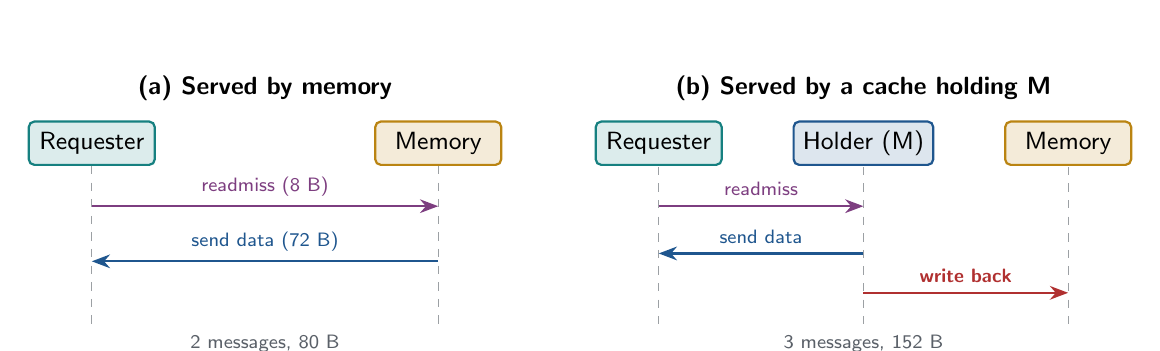
\begin{tikzpicture}[font=\sffamily\scriptsize,
    ag/.style={draw, thick, rounded corners=2pt, minimum width=1.6cm,
               minimum height=0.55cm, font=\sffamily\small},
    m/.style={-{Stealth}, thick}]
  \node[font=\sffamily\bfseries\small] at (2.2,3.6) {(a) Served by memory};
  \node[ag, fill=tealC!15, draw=tealC] (r) at (0,2.9) {Requester};
  \node[ag, fill=amberC!16, draw=amberC] (mm) at (4.4,2.9) {Memory};
  \draw[dashed, coreGrey!60] (r) -- (0,0.6); \draw[dashed, coreGrey!60] (mm) -- (4.4,0.6);
  \draw[m, plumC] (0,2.1) -- node[above]{readmiss (8 B)} (4.4,2.1);
  \draw[m, mesiBlue] (4.4,1.4) -- node[above]{send data (72 B)} (0,1.4);
  \node[text=coreGrey] at (2.2,0.35) {2 messages, 80 B};
  \begin{scope}[xshift=7.2cm]
  \node[font=\sffamily\bfseries\small] at (2.6,3.6) {(b) Served by a cache holding M};
  \node[ag, fill=tealC!15, draw=tealC] (r2) at (0,2.9) {Requester};
  \node[ag, fill=mesiBlue!15, draw=mesiBlue] (o2) at (2.6,2.9) {Holder (M)};
  \node[ag, fill=amberC!16, draw=amberC] (m2) at (5.2,2.9) {Memory};
  \foreach \x in {0,2.6,5.2} \draw[dashed, coreGrey!60] (\x,2.6) -- (\x,0.6);
  \draw[m, plumC] (0,2.1) -- node[above]{readmiss} (2.6,2.1);
  \draw[m, mesiBlue] (2.6,1.5) -- node[above]{send data} (0,1.5);
  \draw[m, alertRed] (2.6,1.0) -- node[above]{\textbf{write back}} (5.2,1.0);
  \node[text=coreGrey] at (2.6,0.35) {3 messages, 152 B};
  \end{scope}
\end{tikzpicture}
\end{bigfig}
\caption[Anatomy of a read miss in MESI]{Two ways MESI serves a read miss. When
another cache holds the block modified, the block is also written back, which
nearly doubles the bytes moved.}
\label{fig:miss-anatomy}
\end{figure}

\Cref{tab:mesi-bill} prices the six-step trace of \cref{tab:trace} under MESI
with the sizes of \cref{tab:msg-classes}. Part~III prices the other protocols.

\begin{table}[htbp]
\centering
\caption{The cost of the six-step trace of \cref{tab:trace} under MESI.}
\label{tab:mesi-bill}
\small
\begin{tabular}{@{}c l l c c c r@{}}
\toprule
Step & Access & MESI action & Control & Data & Write back & Bytes \\
\midrule
1 & P0 reads  & readmiss; memory sends data      & 1 & 1 & 0 & 80 \\
2 & P0 writes & silent \stE$\to$\stM             & 0 & 0 & 0 & 0 \\
3 & P1 reads  & readmiss; P0 sends data, writes back & 1 & 1 & \textbf{1} & 152 \\
4 & P2 reads  & readmiss; data supplied          & 1 & 1 & 0 & 80 \\
5 & P1 writes & \textit{write} invalidates P0, P2 & 1 & 0 & 0 & 8 \\
6 & P0 reads  & readmiss; P1 sends data, writes back & 1 & 1 & \textbf{1} & 152 \\
\midrule
 & \textbf{Total} & & 5 & 4 & \textbf{2} & 472 \\
\bottomrule
\end{tabular}
\end{table}

Of the 472 bytes, 144 (30.5\,\%) are the two writebacks at steps~3 and~6. Both
happen because a core reads a block that another core holds in \stM\ (Chapter~9).

% ---------------------------------------------------------------
\section{A Fourth Kind of Miss: Coherence Misses}
\label{sec:orig-4c}
\sectionmap{[Fourth C [{Three Cs: one core}]
  [Coherence miss: exists only with sharing]]}
\index{coherence miss}%

Sharing adds a fourth kind of miss to the three of \cref{tab:three-c}. A
coherence miss\index{coherence miss} is a miss to a block that was invalidated
because another core wrote it, like P0's read at step~6 of \cref{tab:mesi-bill}.
A larger or more associative cache does not remove it (\cref{fig:4c-tree}). The
protocol sets its price, including whether it also causes a writeback.

\begin{figure}[htbp]
\centering
\adjustbox{max width=0.85\linewidth}{%
\begin{forest}
  decision tree, for tree={l sep=4pt},
  [Has this cache held the block before?
    [Compulsory miss, el=no]
    [Removed by another core's write?, el=yes
      [Coherence miss, el=yes]
      [{Fully associative cache of the\\same size would still hold it?}, el=no
        [Conflict miss, el=yes]
        [Capacity miss, el=no]]]]
\end{forest}}
\caption[Decision tree: classifying a cache miss]{The four kinds of miss. The
coherence miss is the only one caused by sharing.}
\label{fig:4c-tree}
\end{figure}

% ===============================================================
%  Chapter 8 -- How the Cost Grows with Core Count       (Part II)
% ===============================================================
\chapter{How the Cost Grows with Core Count}
\label{ch:scaling}

\begin{figure}[htbp]
\centering
\adjustbox{max width=\linewidth}{%
\begin{forest}
  chapter map,
  [Chapter 8
    [Broadcast {\&} saturation [Lookups grow as N squared] [Bus demand grows with N]]
    [Point-to-point networks [Directory indirection]]
    [Coherence in AMAT [A fourth term]]
    [What this report targets [Not false sharing]]
  ]
\end{forest}}
\caption[]{Structure of Chapter~8. Each section shows one
way coherence cost grows with the number of cores; the last picks the one this
report studies.}
\label{fig:ch8-map}
\end{figure}

The models in this chapter are kept simple on purpose. They show how each cost
grows with the core count, and Part~VI gives measured values.

% ---------------------------------------------------------------
\section{Broadcast and Bus Saturation}
\label{sec:scale-broadcast}
\label{sec:scale-bus}
\sectionmap{[Broadcast cost [Each miss is snooped by N-1 caches]
  [Lookups grow as N squared] [Bus demand grows as N] [Saturation: requests queue]]}
\index{snooping protocol}\index{bus utilisation}%

On a snooping bus every other cache sees each miss and looks up its own tags to
decide whether to respond. With $N$ cores each making $r$ misses per unit time,
the snoop lookups per unit time are
\begin{equation}
  L(N) = N\,r\,(N-1),
  \label{eq:snoop}
\end{equation}
which grows with the square of the core count while useful work grows linearly
(\cref{fig:snoop-growth}). Each lookup costs energy and competes with the core's
own accesses for the tag array.

The bus also carries one message at a time (\cref{sec:coh-snoop}). If each core
keeps the bus busy for a fraction $d$ of the time, the utilisation with $N$ cores
is
\begin{equation}
  U(N) = N\,d
  \label{eq:util}
\end{equation}
until it reaches 100\,\%. Past that point the bus cannot carry the demand,
requests wait in the arbiter's queue and every miss takes longer
(\cref{fig:bus-util}). A core that needs the bus only 10\,\% of the time saturates
it at 10 cores, and every byte a protocol sends without need raises $d$ and brings
saturation closer.

\begin{figure}[htbp]
\centering
\begin{minipage}[t]{0.49\linewidth}\centering
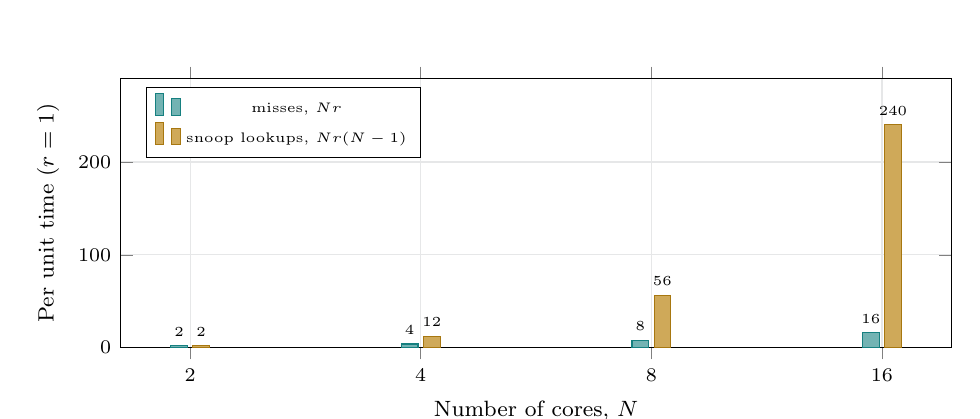
\begin{tikzpicture}
  \begin{axis}[width=\linewidth, height=5cm, ybar, bar width=6pt,
      xlabel={Number of cores, $N$}, ylabel={Per unit time ($r=1$)},
      symbolic x coords={2,4,8,16}, xtick=data, ymin=0, ymax=290,
      legend style={at={(0.03,0.97)}, anchor=north west, font=\tiny},
      nodes near coords, nodes near coords style={font=\tiny},
      grid=major, grid style={coreGrey!15},
      label style={font=\footnotesize}, tick label style={font=\scriptsize}]
    \addplot[fill=tealC!60, draw=tealC] coordinates {(2,2) (4,4) (8,8) (16,16)};
    \addlegendentry{misses, $Nr$}
    \addplot[fill=amberC!70, draw=amberC!90!black] coordinates {(2,2) (4,12) (8,56) (16,240)};
    \addlegendentry{snoop lookups, $Nr(N-1)$}
  \end{axis}
\end{tikzpicture}
\caption[Snoop lookups grow quadratically]{\Cref{eq:snoop}: from 8 to 16 cores
the misses double and the lookups more than quadruple.}
\label{fig:snoop-growth}
\end{minipage}\hfill
\begin{minipage}[t]{0.49\linewidth}\centering
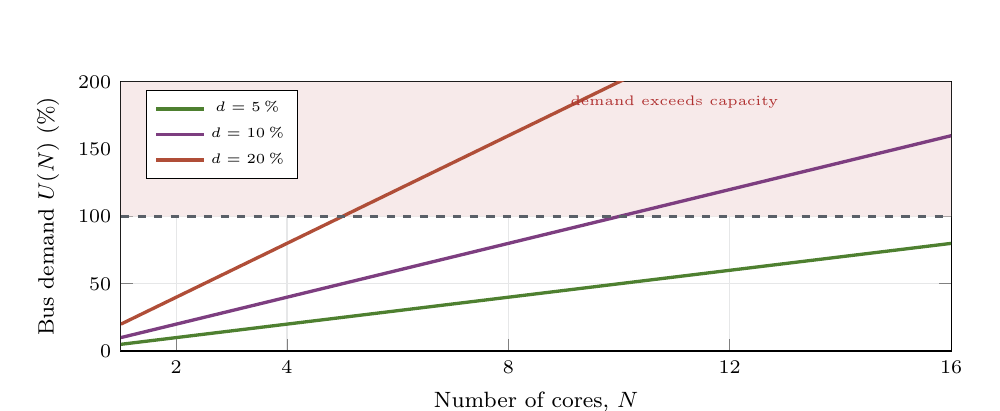
\begin{tikzpicture}
  \begin{axis}[width=\linewidth, height=5cm,
      xlabel={Number of cores, $N$}, ylabel={Bus demand $U(N)$ (\%)},
      xmin=1, xmax=16, ymin=0, ymax=200, xtick={2,4,8,12,16},
      legend style={at={(0.03,0.97)}, anchor=north west, font=\tiny},
      grid=major, grid style={coreGrey!15},
      label style={font=\footnotesize}, tick label style={font=\scriptsize}]
    \addplot[fill=alertRed!10, draw=none, forget plot] coordinates {(1,100) (16,100) (16,200) (1,200)} \closedcycle;
    \addplot[very thick, leafC, domain=1:16] {5*x};   \addlegendentry{$d=5\,\%$}
    \addplot[very thick, plumC, domain=1:16] {10*x};  \addlegendentry{$d=10\,\%$}
    \addplot[very thick, brickC, domain=1:16] {20*x};  \addlegendentry{$d=20\,\%$}
    \addplot[very thick, dashed, coreGrey, domain=1:16, forget plot] {100};
    \node[font=\tiny, text=alertRed] at (axis cs:11,185) {demand exceeds capacity};
  \end{axis}
\end{tikzpicture}
\caption[Bus saturation]{\Cref{eq:util}. Above the dashed line requests queue;
lowering $d$ moves saturation to the right.}
\label{fig:bus-util}
\end{minipage}
\end{figure}

% ---------------------------------------------------------------
\section{Point-to-Point Networks and Directories}
\label{sec:scale-p2p}
\sectionmap{[Beyond the bus [Mesh carries many messages at once]
  [Directory avoids broadcast] [Price: an extra hop]]}
\index{MESI}\index{snooping protocol}\index{directory protocol}\index{network on chip}%

Larger chips replace the bus with a point-to-point network such as a mesh
(\cref{tab:topologies}) and use a directory in place of broadcast
(\cref{sec:coh-dir}). The quadratic snoop cost disappears and many messages can
travel at once, but coherence still costs something. A read miss to a block
modified in another cache now needs three network traversals: request to the
directory, forward to the holder, and reply to the requester. Each crosses several
links of a network whose diameter grows with
$\sqrt{N}$~\cite[\S12.6.3]{sarangi2025basic}. Under MESI the holder also writes
the block back, so the block still moves twice (\cref{ch:scaling-approaches}
draws this transaction).

% ---------------------------------------------------------------
\section{Coherence in the AMAT Equation}
\label{sec:scale-amat}
\sectionmap{[AMAT with coherence [Add a coherence-miss term]
  [Rate grows with sharing and cores] [Cost includes any write back]]}
\index{AMAT}\index{coherence miss}%

\Cref{eq:amat} covers the three kinds of miss of a single core. Adding coherence
misses (\cref{sec:orig-4c}) gives a fourth term,
\begin{equation}
  \mathrm{AMAT} = T_{L1} + m_{L1}\bigl(T_{L2} + m_{L2}\,T_{\mathrm{mem}}\bigr)
                + m_{\mathrm{coh}}\,T_{\mathrm{coh}},
  \label{eq:amat-coh}
\end{equation}
where $m_{\mathrm{coh}}$ is the fraction of accesses that are coherence misses and
$T_{\mathrm{coh}}$ is the time to get the block from another cache, including any
writeback on the way. \Cref{fig:amat-bars} applies \cref{eq:amat-coh} to the
3-cycle example of \cref{sec:cache-hierarchy} with an assumed
$T_{\mathrm{coh}}=60$ cycles and a coherence-miss rate that doubles each time the
core count doubles. Under these assumptions the coherence term is larger than the
whole single-core hierarchy by 16 cores.

\begin{figure}[htbp]
\centering
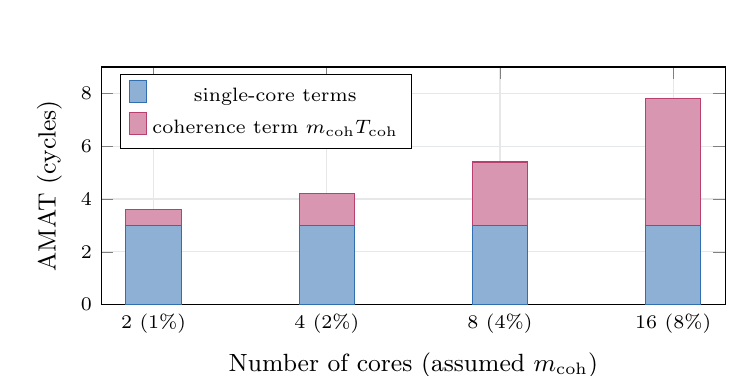
\begin{tikzpicture}
  \begin{axis}[width=9.5cm, height=4.6cm, ybar stacked, bar width=20pt,
      xlabel={Number of cores (assumed $m_{\mathrm{coh}}$)}, ylabel={AMAT (cycles)},
      symbolic x coords={a,b,c,d}, xtick=data, xticklabels={{2 (1\%)},{4 (2\%)},{8 (4\%)},{16 (8\%)}},
      ymin=0, ymax=9,
      legend style={at={(0.03,0.97)}, anchor=north west, font=\scriptsize},
      grid=major, grid style={coreGrey!15},
      label style={font=\small}, tick label style={font=\scriptsize}]
    \addplot[fill=skyC!55, draw=skyC] coordinates
      {(a,3) (b,3) (c,3) (d,3)};
    \addlegendentry{single-core terms}
    \addplot[fill=roseC!55, draw=roseC] coordinates
      {(a,0.6) (b,1.2) (c,2.4) (d,4.8)};
    \addlegendentry{coherence term $m_{\mathrm{coh}}T_{\mathrm{coh}}$}
  \end{axis}
\end{tikzpicture}
\caption[AMAT with a coherence term]{\Cref{eq:amat-coh} with illustrative values.
A smaller $T_{\mathrm{coh}}$, for example one without a writeback on every
coherence transfer, shrinks the pink bars.}
\label{fig:amat-bars}
\end{figure}

% ---------------------------------------------------------------
\section{What This Report Targets}
\label{sec:scale-target}
\label{sec:scale-false}
\sectionmap{[Target [Many sources of coherence cost]
  [Most are inherent to sharing] [{False sharing: not targeted}] [One is avoidable in principle]]}
\index{MESI}\index{MSI}\index{false sharing}%

Coherence works on blocks. If two cores write different variables that happen to
share a block, each write invalidates the other core's copy and the block moves
back and forth even though no data is shared. This false
sharing\index{false sharing} causes real traffic, but it comes from writes on both
sides, and every MSI-family protocol must transfer ownership on each of them, so
we leave it out.

\Cref{fig:overhead-map} collects the costs from Chapters~7 and~8. Most come with
sharing itself: a block has to move when another core needs it, and other copies
have to be invalidated when a core writes. The last one is different. When a core
reads a block that another core holds modified, MESI sends the block to the
reader, which is required, and also writes it back to memory, which no rule of
coherence requires. Chapter~9 looks at that writeback.

\begin{figure}[htbp]
\centering
\adjustbox{max width=0.85\linewidth}{%
\begin{forest}
  for tree={
    grow'=0, parent anchor=east, child anchor=west, anchor=west,
    align=center, font=\sffamily\small, draw, thick, rounded corners=3pt,
    inner sep=4pt, l sep+=14pt, s sep+=2pt,
    edge={thick, coreGrey!60, -{Stealth[length=5pt]}},
    fill=coreGrey!8, draw=coreGrey!60, text=coreGrey
  },
  [Coherence cost, fill=mesiBlue, draw=mesiBlue, text=white, font=\sffamily\bfseries\small
    [Snoop lookups on every miss]
    [Bus or network contention]
    [Invalidations on writes]
    [Cache-to-cache data transfers]
    [False sharing]
    [Write backs when a modified\\block is read by another core,
      fill=moesiOrange, draw=moesiOrange, text=white, font=\sffamily\bfseries\small
      [{Targeted by\\this report}, fill=moesiOrange!12, draw=moesiOrange, text=black]]
  ]
\end{forest}}
\caption[Sources of coherence cost]{Sources of coherence cost found in
Chapters~7 and~8. The highlighted one is studied in this report.}
\label{fig:overhead-map}
\end{figure}

% ===============================================================
%  Chapter 9 -- Forced Writebacks on Dirty Sharing       (Part II)
% ===============================================================
\chapter{Forced Writebacks on Dirty Sharing}
\label{ch:dirty-sharing}

\begin{figure}[htbp]
\centering
\adjustbox{max width=\linewidth}{%
\begin{forest}
  chapter map,
  [Chapter 9
    [The transaction [Three messages]]
    [The root cause [S must be clean]]
    [Wasted write backs [Superseded writes]]
    [Sharing patterns [Four patterns] [Producer--consumer model]]
  ]
\end{forest}}
\caption[]{Structure of Chapter~9: one transaction, the
design rule behind it, and its cost in the sharing patterns where it occurs.}
\label{fig:ch9-map}
\end{figure}

% ---------------------------------------------------------------
\section{The Transaction}
\label{sec:dirty-transaction}
\sectionmap{[Transaction [Cache A holds M] [Cache B reads] [A sends data to B]
  [A also writes back] [Both end in S]]}
\index{MESI}\index{dirty sharing}%

In this report \emph{dirty sharing}\index{dirty sharing} means one situation: a
block is modified (dirty) in one cache and another cache reads it, so it becomes
shared. \Cref{fig:dirty-transaction} shows what MESI does. The holder sends the
data to the reader, writes the block back to memory, and both caches end in \stS.
The reader needs the data, so the transfer cannot be avoided. This chapter is
about the writeback.

\begin{figure}[htbp]
\centering
\begin{bigfig}[0.85]
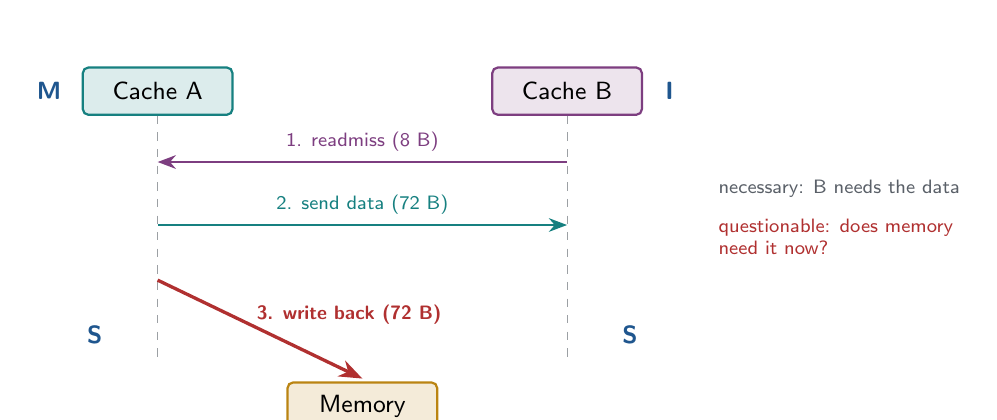
\begin{tikzpicture}[font=\sffamily\scriptsize,
    ag/.style={draw, thick, rounded corners=2pt, minimum width=1.9cm,
               minimum height=0.6cm, align=center, font=\sffamily\small},
    msg/.style={-{Stealth}, thick}, st/.style={font=\sffamily\bfseries\small}]
  \node[ag, fill=tealC!15, draw=tealC] (A) at (0,0) {Cache A};
  \node[ag, fill=plumC!14, draw=plumC] (B) at (5.2,0) {Cache B};
  \node[ag, fill=amberC!16, draw=amberC] (M) at (2.6,-4.0) {Memory};
  \draw[dashed, coreGrey!60] (A) -- (0,-3.4);
  \draw[dashed, coreGrey!60] (B) -- (5.2,-3.4);
  \node[st, text=mesiBlue, anchor=east] at (-1.1,0) {\stM};
  \draw[msg, plumC] (5.2,-0.9) -- node[above]{1. readmiss (8 B)} (0,-0.9);
  \draw[msg, tealC] (0,-1.7) -- node[above]{2. send data (72 B)} (5.2,-1.7);
  \draw[msg, alertRed, very thick] (0,-2.4) -- node[right=6pt, pos=0.35, text=alertRed]{\textbf{3. write back (72 B)}} (2.6,-3.65);
  \node[st, text=mesiBlue] at (-0.8,-3.1) {\stS};
  \node[st, text=mesiBlue] at (6.0,-3.1) {\stS};
  \node[st, text=mesiBlue] at (6.5,0) {\stI};
  \node[text=coreGrey, align=left, anchor=west] at (7.0,-1.6)
       {necessary: B needs the data\\[6pt]\textcolor{alertRed}{questionable: does memory}\\\textcolor{alertRed}{need it now?}};
\end{tikzpicture}
\end{bigfig}
\caption[Dirty sharing in MESI]{Dirty sharing under MESI. Cache~A holds the block
in \stM\ and cache~B reads it. Message~2 is needed for correctness. Message~3 is
what this report calls a forced writeback.}
\label{fig:dirty-transaction}
\end{figure}

% ---------------------------------------------------------------
\section{The Root Cause: The Shared State Must Be Clean}
\label{sec:dirty-root}
\sectionmap{[Root cause [S blocks are evicted silently] [So S must match memory]
  [So M to S must update memory] [The write back follows]]}
\index{MESI}\index{MSI}\index{forced writeback}\index{coherence axioms}%

The prescribed textbook gives the reason when it describes how MSI answers a
\textit{readmiss} for a block in \stM:

\begin{quote}
``We assume that we can seamlessly evict a block in the S state. Hence, it is
necessary to write the data to the lower level before moving to the S
state.''~\cite[\S12.4.6, p.~602]{sarangi2025basic}
\end{quote}

MESI keeps this rule. \Cref{fig:root-chain} sets out the reasoning. A cache must
be able to drop an \stS\ block without telling anyone, which is what makes \stS\
cheap. A block can be dropped silently only if its data also survives somewhere
else, namely in memory. Every \stS\ block must therefore match memory, and a
block moving from \stM\ to \stS\ must update memory first.

\begin{figure}[htbp]
\centering
\begin{bigfig}[0.95]
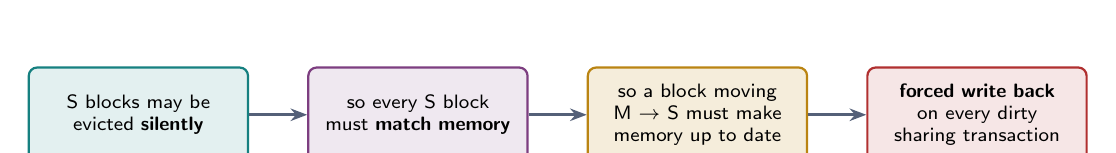
\begin{tikzpicture}[font=\sffamily\scriptsize,
    s/.style={draw, thick, rounded corners=3pt, align=center, text width=2.55cm,
              minimum height=1.2cm},
    a/.style={-{Stealth[length=6pt]}, very thick, slateC}]
  \node[s, fill=tealC!12, draw=tealC] (r1) at (0,0) {S blocks may be\\evicted \textbf{silently}};
  \node[s, fill=plumC!12, draw=plumC] (r2) at (3.55,0) {so every S block\\must \textbf{match memory}};
  \node[s, fill=amberC!15, draw=amberC] (r3) at (7.1,0) {so a block moving\\M $\to$ S must make\\memory up to date};
  \node[s, fill=alertRed!12, draw=alertRed] (r4) at (10.65,0) {\textbf{forced write back}\\on every dirty\\sharing transaction};
  \draw[a] (r1) -- (r2); \draw[a] (r2) -- (r3); \draw[a] (r3) -- (r4);
\end{tikzpicture}
\end{bigfig}
\caption[Why MESI writes back on dirty sharing]{The reasoning behind the forced
writeback. The rule on the left makes shared blocks cheap to evict; the cost on
the right is paid on every dirty sharing transaction.}
\label{fig:root-chain}
\end{figure}

\begin{keybox}[The root cause]
Neither coherence axiom requires the \gls{fwb}\index{forced writeback}. It follows
from a design rule, that shared blocks are always clean, which was chosen so that
shared blocks can be evicted without a message.
\end{keybox}

No correct protocol can remove a cost that the axioms require, but a cost that
comes from a design rule can be removed by changing the rule, as long as the
axioms still hold. The rest of this report asks whether that change pays off.

% ---------------------------------------------------------------
\section{When the Writeback Is Wasted}
\label{sec:dirty-wasted}
\sectionmap{[Wasted write backs [Producer writes again] [Memory copy is out of date again]
  [Earlier write back was superseded] [Only the last one is needed]]}
\index{MESI}\index{forced writeback}%

A forced writeback is useful only if someone reads memory's copy before it goes
out of date. Take a producer core that keeps updating a block and a consumer core
that reads each new version (\cref{fig:wasted-timeline}). Under MESI every consumer
read forces a writeback, and every new producer write makes the copy just written
to memory out of date. Memory ends up with its final value only from the last
writeback before the block leaves the caches.

\begin{figure}[htbp]
\centering
\begin{bigfig}
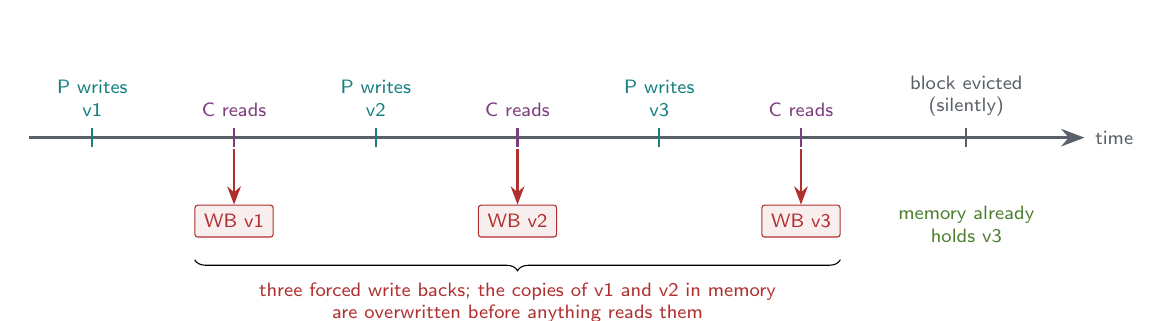
\begin{tikzpicture}[font=\sffamily\scriptsize]
  \draw[very thick, coreGrey, -{Stealth}] (0,0) -- (13.4,0) node[right]{time};
  \foreach \x/\lab/\col in {0.8/{P writes\\v1}/tealC, 2.6/{C reads}/plumC,
                            4.4/{P writes\\v2}/tealC, 6.2/{C reads}/plumC,
                            8.0/{P writes\\v3}/tealC, 9.8/{C reads}/plumC,
                            11.9/{block evicted\\(silently)}/coreGrey} {
    \draw[\col, thick] (\x,-0.12) -- (\x,0.12);
    \node[above, align=center, text=\col] at (\x,0.15) {\lab};
  }
  \foreach \x/\v in {2.6/v1,6.2/v2,9.8/v3} {
    \draw[-{Stealth}, alertRed, thick] (\x,-0.15) -- (\x,-0.85);
    \node[draw, alertRed, rounded corners=1pt, fill=alertRed!8, below] at (\x,-0.85) {WB \v};
  }
  \node[text=leafC, align=center] at (11.9,-1.1) {memory already\\holds v3};
  \draw[decorate, decoration={brace, amplitude=4pt, mirror}] (2.1,-1.55) -- (10.3,-1.55)
    node[midway, below=5pt, text=alertRed, align=center]{three forced write backs; the copies of v1 and v2 in memory\\are overwritten before anything reads them};
\end{tikzpicture}
\end{bigfig}
\caption[Superseded writebacks]{A producer (P) and consumer (C) under MESI. Each
consumer read forces a writeback and the next producer write makes it out of date.
Only the writeback of v3 is still current when the block is evicted.}
\label{fig:wasted-timeline}
\end{figure}

Here two of the three forced writebacks are overwritten before memory's copy is
used. With $k$ rounds, $k-1$ of the $k$ forced writebacks are overwritten, and one
write to memory would have been enough.

% ---------------------------------------------------------------
\section{Sharing Patterns}
\label{sec:dirty-patterns}
\sectionmap{[Patterns [Private: never shared] [Read-only: never written]
  [Producer-consumer: one writer] [Migratory: writers take turns]]}
\index{MESI}\index{forced writeback}\index{sharing patterns!producer--consumer}%

Whether forced writebacks happen depends on how a program shares data.
Shared-memory programs are usually described by four sharing
patterns~\cite{culler1999parallel}\index{sharing patterns}. \Cref{fig:pattern-tree}
shows how to tell them apart and \cref{tab:patterns} gives the forced-writeback
cost of each under MESI.

\begin{figure}[htbp]
\centering
\adjustbox{max width=0.8\linewidth}{%
\begin{forest}
  decision tree,
  [Is the block used by\\more than one core?
    [Private, el=no]
    [Is it ever\\written?, el=yes
      [Read-only\\shared, el=no]
      [Do several cores\\write it in turn?, el=yes
        [Producer--consumer\\one writer and\\several readers, el=no]
        [Migratory\\each core reads\\then writes, el=yes]]]]
\end{forest}}
\caption[Decision tree: classifying a sharing pattern]{The four sharing patterns.
Only the two on the bottom row have a block that is modified in one cache and then
read by another.}
\label{fig:pattern-tree}
\end{figure}

\begin{table}[htbp]
\centering
\caption{The four sharing patterns and their forced-writeback cost under MESI.}
\label{tab:patterns}
\small
\begin{tabular}{@{}l p{4.6cm} p{4.4cm}@{}}
\toprule
Pattern & Example & Forced write backs (MESI) \\
\midrule
Private & a thread's own stack and locals & none: never shared \\
Read-only shared & an input matrix read by every thread & none: never modified \\
Producer--consumer & the \texttt{partial[]} results of \cref{lst:omp}, read
  by the combining thread & one per value produced \\
Migratory & a counter that each thread reads and then updates in turn &
  one per hand-off that begins with a read \\
\bottomrule
\end{tabular}
\end{table}

\label{sec:dirty-model}
So the size of the cost depends on the workload as much as on the protocol. A
program that mostly uses private and read-only data never pays it, and a pipeline
of producer and consumer threads pays it on every hand-off. For one producer and
$C$ consumers sharing a block under MESI in steady state, each round has the
producer's write invalidating the consumers (8\,B), the first consumer's read
missing, getting the data and forcing a writeback ($8+72+72=152$\,B), and each of
the other $C-1$ consumers missing and getting the data ($80$\,B each). The bytes
per round and the share of them that is the forced writeback are
\begin{equation}
  B(C) = 160 + 80\,(C-1), \qquad
  F(C) = \frac{72}{B(C)}
  \label{eq:pc-model}
\end{equation}

\begin{figure}[htbp]
\centering
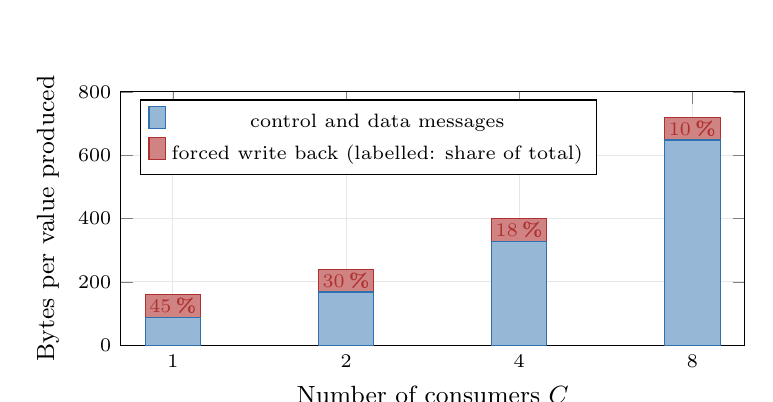
\begin{tikzpicture}
  \begin{axis}[width=9.5cm, height=4.8cm, ybar stacked, bar width=20pt,
      xlabel={Number of consumers $C$}, ylabel={Bytes per value produced},
      symbolic x coords={1,2,4,8}, xtick=data, ymin=0, ymax=800,
      legend style={at={(0.03,0.97)}, anchor=north west, font=\scriptsize},
      grid=major, grid style={coreGrey!15},
      label style={font=\small}, tick label style={font=\scriptsize}]
    \addplot[fill=skyC!50, draw=skyC] coordinates {(1,88) (2,168) (4,328) (8,648)};
    \addlegendentry{control and data messages}
    \addplot[fill=alertRed!60, draw=alertRed,
             nodes near coords={\pgfmathprintnumber[fixed,precision=0]{\pgfplotspointmeta}\,\%},
             point meta=explicit, nodes near coords style={font=\scriptsize\bfseries, text=alertRed}]
      coordinates {(1,72) [45] (2,72) [30] (4,72) [18] (8,72) [10]};
    \addlegendentry{forced write back (labelled: share of total)}
  \end{axis}
\end{tikzpicture}
\caption[Forced writeback traffic in producer--consumer sharing]{\Cref{eq:pc-model}
for 1, 2, 4 and 8 consumers under MESI. The forced writeback is 72 bytes per round,
so its share is largest (45\,\%) when one consumer reads each value.}
\label{fig:pc-model}
\end{figure}

The share of traffic taken by the forced writeback therefore changes with the
workload (\cref{fig:pc-model}). It is largest in one-to-one producer--consumer
hand-offs and shrinks when many consumers read each value, so a study of the
problem has to vary the sharing pattern as well as the core count.

\label{sec:dirty-memory}
A forced writeback is paid for twice. It occupies the bus or network, which raises
the per-core demand $d$ of \cref{eq:util}, and it writes to the LLC or DRAM, using
memory bandwidth that all cores share and that does not grow with the core count.
When the writeback is later overwritten (\cref{sec:dirty-wasted}), neither cost
buys anything.

% ===============================================================
%  Chapter 10 -- Problem Statement                       (Part II)
% ===============================================================
\chapter{Problem Statement: The Cost of Forced Writebacks on Dirty Sharing}
\label{ch:problem}

\begin{figure}[htbp]
\centering
\adjustbox{max width=\linewidth}{%
\begin{forest}
  chapter map,
  [Chapter 10
    [The problem [In words] [Formally]]
    [Scope {\&} assumptions]
    [Research questions [RQ1 to RQ4]]
    [Requirements for a solution [Decision tree]]
  ]
\end{forest}}
\caption[]{Structure of Chapter~10: the problem in words
and formally, its scope, and the research questions Parts~III to~VI answer.}
\label{fig:ch10-map}
\end{figure}

% ---------------------------------------------------------------
\section{The Problem}
\label{sec:prob-sentence}
\label{sec:prob-formal}
\sectionmap{[The problem [MESI writes back on every dirty sharing transfer]
  [Not required by the axioms] [{Measured by B, T, AMAT and F}]]}
\index{MESI}\index{forced writeback}\index{dirty sharing}\index{write-back cache}\index{AMAT}\index{snooping protocol}\index{directory protocol}\index{sharing patterns!producer--consumer}\index{coherence axioms}%

\begin{problembox}[Problem Statement]
In a multicore processor that uses MESI, whenever one core reads a block that
another core holds modified, the protocol writes the block back to memory as well
as supplying it to the reader. The coherence axioms do not require this writeback;
MESI's rule that shared blocks are clean does. The writeback uses interconnect and
memory bandwidth, is often overwritten before memory's copy is read, and its share
of total traffic varies widely with the sharing pattern. We ask how much the
forced writeback costs on 2 to 16 cores, how much of that cost a coherent protocol
can remove, and whether the benefit of removing it can be predicted from a
workload's behaviour under MESI alone.
\end{problembox}

The system is a chip with $N\in\{2,4,8,16\}$ cores, each with a private
write-back L1 cache, sharing an LLC and main memory over a snooping bus or a
directory network, with 64-byte blocks. The workload $W$ is a shared-memory
parallel program run with one thread per core. For a protocol $P$ on $W$ with
$N$ cores we define
\begin{align*}
  B_{\mathrm{tot}}(P,W,N) &= \text{total bytes moved by coherence messages,}\\
  B_{\mathrm{fwb}}(P,W,N) &= \text{bytes moved by forced writebacks
      (\stM$\to$\stS\ on a remote read),}\\
  T(P,W,N) &= \text{execution time,}\qquad
  \mathrm{AMAT}(P,W,N) \text{ as in \cref{eq:amat-coh},}
\end{align*}
and the forced-writeback fraction of a workload as
\begin{equation}
  F(W,N) = \frac{B_{\mathrm{fwb}}(\mathrm{MESI},W,N)}{B_{\mathrm{tot}}(\mathrm{MESI},W,N)}.
  \label{eq:fwb-fraction}
\end{equation}
$F$ is 30.5\,\% for the trace of \cref{tab:mesi-bill} and between 10\,\% and
45\,\% for the producer--consumer model of \cref{eq:pc-model}. For each $W$ and
$N$ the task is (i)~to measure $F(W,N)$; (ii)~for any protocol $P$ that removes
forced writebacks and keeps both axioms, to measure the change in
$B_{\mathrm{tot}}$, $T$ and AMAT relative to MESI; and (iii)~to find out whether
that change can be predicted from quantities measured under MESI alone.

% ---------------------------------------------------------------
\section{Scope and Assumptions}
\label{sec:prob-scope}
\sectionmap{[Scope [MSI-family write-invalidate] [2 to 16 cores]
  [Consistency model fixed] [OpenMP workloads]]}
\index{MSI}\index{forced writeback}\index{write-back cache}\index{snooping protocol}\index{directory protocol}\index{write-invalidate}\index{false sharing}\index{OpenMP}\index{memory consistency}\index{verification}%

We chose these assumptions so that the forced writeback is the only variable of
interest.
\begin{itemize}[itemsep=1pt]
  \item Protocols: the write-invalidate MSI family (Chapter~5) in snooping and
    directory forms.
  \item Caches: private write-back L1 caches with 64-byte blocks and a shared LLC
    (\cref{sec:cache-private}).
  \item Scale: 2, 4, 8 and 16 cores, where both snooping and directories are
    realistic (\cref{fig:choose-tree}).
  \item Consistency: fixed and not studied (\cref{sec:coh-consistency}).
  \item Workloads: shared-memory C programs parallelised with OpenMP
    (\cref{sec:par-threads}), including kernels built to show each sharing pattern
    of \cref{tab:patterns}.
  \item Out of scope: false sharing (\cref{sec:scale-false}), message passing and
    formal verification.
\end{itemize}

% ---------------------------------------------------------------
\section{Research Questions}
\label{sec:prob-rq}
\sectionmap{[Research questions [RQ1: how big is F] [RQ2: does traffic saved become time saved]
  [RQ3: can it be predicted] [RQ4: when does removing it hurt]]}

The problem splits into four research questions (\cref{tab:rq}).

\begin{table}[htbp]
\centering
\caption{Research questions and where each is answered.}
\label{tab:rq}
\small
\begin{tabular}{@{}l p{8.4cm} l@{}}
\toprule
 & Question & Answered in \\
\midrule
RQ1 & How large is the forced-writeback fraction $F(W,N)$ for realistic
  workloads, and how does it change from 2 to 16 cores? & Part VI \\
RQ2 & When a protocol removes forced writebacks, does the saved traffic turn
  into saved execution time, or is it hidden while the interconnect is lightly
  loaded? & Part VI \\
RQ3 & Can the benefit be predicted from a workload's behaviour under MESI,
  before the other protocol is built? & Parts IV and VI \\
RQ4 & Are there conditions, such as a small LLC, under which deferring the
  writeback costs more than it saves? & Parts IV and VI \\
\bottomrule
\end{tabular}
\end{table}

% ---------------------------------------------------------------
\section{Requirements for Any Solution}
\label{sec:prob-requirements}
\label{sec:prob-bridge}
\sectionmap{[Requirements [Keep completion] [Keep order]
  [Remove the forced write back] [Keep MESI's gains]]}
\index{MESI}\index{MOESI}\index{MESIF}\index{Owned state}\index{forced writeback}\index{directory protocol}\index{token coherence}\index{write-update}\index{coherence axioms}%

A candidate solution in Part~III must meet four requirements, applied in order
in \cref{fig:req-tree}. The first two are the coherence axioms. The third is the
problem itself. The fourth stops a solution from trading one inefficiency for
another. Part~III judges the existing answers against them: the Owned state of
MOESI, which removes the forced writeback directly; write-update protocols, which
avoid invalidation; the Forward state of MESIF, which targets a different cost of
sharing; and directories and token coherence, which change how the cost is paid.

\begin{figure}[htbp]
\centering
\adjustbox{max width=0.85\linewidth}{%
\begin{forest}
  decision tree,
  [Does every deferred write\\still reach memory eventually?\\(completion axiom)
    [Rejected:\\loses writes, el=no]
    [Do all caches still see writes\\to a block in one order?\\(order axiom), el=yes
      [Rejected:\\incoherent, el=no]
      [Does it remove the write back\\on a remote read of an M block?, el=yes
        [Not a solution\\to this problem, el=no]
        [Does it keep MESI's silent\\E-to-M upgrade?, el=yes
          [Weaker candidate, el=no]
          [Candidate for\\Part III, el=yes]]]]]
\end{forest}}
\caption[Decision tree: requirements for a solution]{The four requirements for a
solution, applied in order. Only solutions that reach the bottom-right box are
full candidates in Part~III.}
\label{fig:req-tree}
\end{figure}


% ---------------------------------------------------------------
%  Parts III--VII
% ===============================================================
%  PART III -- Existing Solutions to the Forced-Writeback Problem
%  Chapters 11--14. Uses the shared preamble and refs.bib.
% ===============================================================

\part{Existing Solutions to the Forced-Writeback Problem}
\label{part:solutions}

\begin{center}
\adjustbox{max width=\linewidth}{%
\begin{forest}
  part map,
  [Part III
    [Ch.~11: Owner-Based Solutions
      [Berkeley ownership] [MOESI and the O state] [Limits of ownership]]
    [Ch.~12: Other Extensions
      [Write-update: Dragon {\&} Firefly] [MESIF: the F state]]
    [Ch.~13: Scaling Approaches
      [Directories: DASH] [Token coherence]]
    [Ch.~14: Comparative Analysis
      [Mechanisms] [Traffic model] [Published evaluations] [Research gap]]
  ]
\end{forest}}
\end{center}

\begin{keybox}[What Part III does]
Part~III reviews published approaches against the problem of Chapter~10. For each
one we ask what it does when a block held in \stM\ is read by another cache, what
that costs, and whether it meets the requirements of \cref{fig:req-tree}. The
approaches fall into three classes. Direct solutions change the block states so
that modified data can be shared without updating memory (Chapter~11).
Alternative strategies change how shared data is propagated or forwarded, and
affect the forced writeback as a side effect (Chapter~12). Organisations change
how requests travel and are ordered, and leave the writeback to the state
protocol that runs on top of them (Chapter~13). Chapter~14 compares all three.
\end{keybox}

% ===============================================================
%  Chapter 11 -- Owner-Based Solutions: MOESI and the Berkeley Protocol
% ===============================================================
\chapter{Owner-Based Solutions: MOESI and the Berkeley Protocol}
\label{ch:owner}
\index{MOESI}\index{Berkeley protocol}\index{owner}%

\begin{figure}[htbp]
\centering
\adjustbox{max width=\linewidth}{%
\begin{forest}
  chapter map,
  [Chapter 11
    [Motivation [Supplier vs owner vs memory] [Clean-S is a choice]]
    [Berkeley protocol [Shared-Dirty owner] [Invalidate before write]]
    [MOESI [Three attributes] [M to O] [Futurebus signals]]
    [Comparison {\&} limits [Table A] [Deferred not removed]]
  ]
\end{forest}}
\caption[]{Structure of Chapter~11. These are the only
approaches in Part~III designed to let modified data be shared without first
updating memory.}
\label{fig:ch11-map}
\end{figure}

% ---------------------------------------------------------------
\section{Motivation for Owner-Based Protocols}
\label{sec:own-motivation}
\sectionmap{[Motivation [Three roles for one block] [MESI merges them on M to S]
  [Ownership separates responsibility from memory]]}
\index{MESI}\index{MOESI}\index{Berkeley protocol}\index{coherence axioms}\index{owner}%

A cached block involves three roles: the supplier, which gives the current data
to a requester; the responsible party, which must make sure the current data
reaches memory in the end; and memory, which may or may not hold the current
value. Under MESI the responsible party is the one cache holding the block in
\stM\ or, if there is none, memory. A block in \stS\ is therefore valid only if
memory is current (the clean-shared rule of \cref{sec:dirty-root}), and the
transition $\stM\to\stS$ has to hand responsibility to memory by writing the block
back. As an invariant, let $\mathcal{O}(b)$ be the set of caches responsible for
block $b$. Every protocol in this chapter keeps
\begin{equation}
  |\mathcal{O}(b)| \le 1
  \qquad\text{and}\qquad
  \mathcal{O}(b) = \varnothing \;\Rightarrow\; \text{memory holds the current value of } b.
  \label{eq:owner-invariant}
\end{equation}
MESI also requires that no other valid copy exist while $\mathcal{O}(b)$ is
non-empty, and it is this extra rule, not \cref{eq:owner-invariant}, that forces
the writeback. Neither coherence axiom (\cref{sec:coh-meaning}) needs memory to be
current while some cache is still responsible for the block. An owner-based
protocol drops only the extra rule: one cache, the \gls{owner}, stays responsible
for a modified block while other caches hold read-only copies, and memory is
updated when ownership ends (\cref{fig:roles}).

\begin{figure}[htbp]
\centering
\begin{bigfig}[0.88]
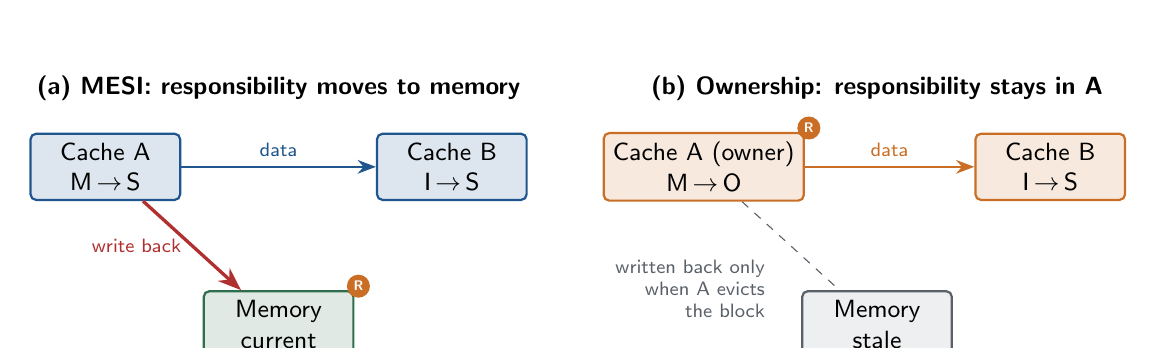
\begin{tikzpicture}[font=\sffamily\scriptsize,
    ag/.style={draw, thick, rounded corners=2pt, minimum width=1.9cm,
               minimum height=0.65cm, align=center, font=\sffamily\small},
    resp/.style={circle, fill=moesiOrange, text=white, font=\sffamily\bfseries\tiny,
                 inner sep=1.2pt},
    m/.style={-{Stealth}, thick}]
  \node[font=\sffamily\bfseries\small] at (2.2,3.0) {(a) MESI: responsibility moves to memory};
  \node[ag, fill=mesiBlue!15, draw=mesiBlue] (A) at (0,2.0) {Cache A\\\stM$\,\to\,$\stS};
  \node[ag, fill=mesiBlue!15, draw=mesiBlue] (B) at (4.4,2.0) {Cache B\\\stI$\,\to\,$\stS};
  \node[ag, fill=memGreen!15, draw=memGreen] (M) at (2.2,0.0) {Memory\\current};
  \draw[m, mesiBlue] (A) -- node[above]{data} (B);
  \draw[m, alertRed, very thick] (A) -- node[left, text=alertRed]{write back} (M);
  \node[resp] at ($(M.north east)+(0.05,0.05)$) {R};
  \begin{scope}[xshift=7.6cm]
  \node[font=\sffamily\bfseries\small] at (2.2,3.0) {(b) Ownership: responsibility stays in A};
  \node[ag, fill=moesiOrange!15, draw=moesiOrange] (A2) at (0,2.0) {Cache A (owner)\\\stM$\,\to\,$\stO};
  \node[ag, fill=moesiOrange!15, draw=moesiOrange] (B2) at (4.4,2.0) {Cache B\\\stI$\,\to\,$\stS};
  \node[ag, fill=coreGrey!10, draw=coreGrey] (M2) at (2.2,0.0) {Memory\\stale};
  \draw[m, moesiOrange] (A2) -- node[above]{data} (B2);
  \draw[dashed, coreGrey] (A2) -- (M2);
  \node[text=coreGrey, align=right, anchor=east] at (0.9,0.45) {written back only\\when A evicts\\the block};
  \node[resp] at ($(A2.north east)+(0.05,0.05)$) {R};
  \end{scope}
\end{tikzpicture}
\end{bigfig}
\caption[Responsibility for a dirty block after a remote read]{Where responsibility
(R) for a modified block sits after another cache reads it. Under MESI it passes to
memory through a writeback; under ownership it stays with the supplier and memory
stays stale.}
\label{fig:roles}
\end{figure}

The idea is older than the MOESI name. Archibald and Baer, describing the
protocols of the early 1980s, say the Berkeley protocol ``uses the idea of
ownership'', and the owner they define is the cache that has the block in
\textsc{Dirty} or \textsc{Shared-Dirty}~\cite[pp.~277--278]{archibald1986evaluation}.

% ---------------------------------------------------------------
\section{The Berkeley Ownership Protocol}
\label{sec:own-berkeley}
\sectionmap{[Berkeley protocol [Designed with its controller chip] [Four states]
  [Owner supplies and keeps ownership] [Memory updated on replacement]
  [Invalidation before every non-owner write]]}
\index{MESI}\index{MSI}\index{Exclusive state}\index{forced writeback}\index{snooping protocol}\index{Berkeley protocol}\index{coherence axioms}\index{memory consistency}\index{owner}%

Katz, Eggers, Wood, Perkins and Sheldon designed the Berkeley protocol and
published it as a technical report~\cite{katz1984implementing} and at
ISCA~1985~\cite{katz1985implementing}. They call it an ``ownership-based
multiprocessor cache consistency protocol''. The report presents it together
with a cache controller meant to fit on one VLSI chip, spends much of its length
on making the controller's concurrent operations safe, and takes that design down
to a CMOS layout~\cite{katz1984implementing}. The state set is therefore one a
snooping controller of the early 1980s could actually implement. We could not read
the original report in full (see the note at the end of this chapter), so the
states below follow Archibald and Baer's
description~\cite[pp.~277--278]{archibald1986evaluation} (\cref{tab:berkeley-states}).
There is no counterpart of \stE: a block read when no other cache holds it enters
\textsc{Valid}, as in MSI.

\begin{table}[htbp]
\centering
\caption{States of the Berkeley protocol as described by Archibald and
Baer~\cite[pp.~277--278]{archibald1986evaluation}.}
\label{tab:berkeley-states}
\small
\begin{tabular}{@{}l L{4.2cm} c c l@{}}
\toprule
State & Meaning & Owner? & Other copies? & Nearest MOESI state \\
\midrule
\textsc{Invalid}      & no valid copy & --- & --- & \stI \\
\textsc{Valid}        & read-only copy; not responsible for memory & no & possibly & \stS \\
\textsc{Shared-Dirty} & modified; owned by this cache & yes & possibly & \stO \\
\textsc{Dirty}        & modified; owned by this cache, sole copy & yes & no & \stM \\
\bottomrule
\end{tabular}
\end{table}

On a miss to a block that another cache holds in \textsc{Dirty} or
\textsc{Shared-Dirty}, the owning cache ``must supply the block contents directly
to the other cache''. The owner then holds the block in \textsc{Shared-Dirty} and
the requester in \textsc{Valid}~\cite[p.~278]{archibald1986evaluation}. Memory is
not written, because a modified block is not written back on becoming
shared~\cite[p.~277]{archibald1986evaluation}, so responsibility stays with the
supplier as in \cref{fig:roles}(b). Memory catches up only on replacement: ``A
block in either state \textsc{Shared-Dirty} or \textsc{Dirty} must be written back
to main memory if it is selected for
replacement''~\cite[p.~277]{archibald1986evaluation}.

A cache becomes the owner by writing. A write hit to a block in \textsc{Valid} or
\textsc{Shared-Dirty} requires that ``an invalidation signal must be sent on the
bus before the write is allowed to proceed''. Every other copy is invalidated and
the writer's block becomes \textsc{Dirty}~\cite[p.~278]{archibald1986evaluation}.
If another cache was the owner, its duty ends with the invalidation, since the new
write replaces its data, and no writeback is needed.

On the transaction of \cref{fig:dirty-transaction} the Berkeley protocol removes
the forced writeback completely: one request and one data transfer replace MESI's
request, data transfer and writeback. The cost shows up elsewhere. With no \stE,
the first write to any block fetched from memory needs a bus invalidation even
when no other cache holds the block, which is the inefficiency MESI was designed
to remove (\cref{sec:fam-mesi}). Against \cref{fig:req-tree}, Berkeley keeps both
axioms and removes the forced writeback but loses MESI's silent upgrade, so it is
a ``weaker candidate''.

% ---------------------------------------------------------------
\section{MOESI: The Owned State}
\label{sec:own-moesi}
\sectionmap{[MOESI [A class of compatible protocols] [Three attributes per line]
  [Intervention: O and M supply data] [Memory updated on replacement]]}
\index{MESI}\index{MOESI}\index{Owned state}\index{Exclusive state}\index{forced writeback}\index{Berkeley protocol}\index{Dragon protocol}\index{Firefly protocol}\index{Illinois protocol}\index{Futurebus}\index{owner}%

Sweazey and Smith defined a whole class of protocols. As
long as every cache ``uses a protocol from the class we define, the overall memory
system state will remain consistent''~\cite[p.~415]{sweazey1986moesi}, and they
showed how the IEEE Futurebus could support any member of the class. Each cache
may pick, at any moment, any action that some protocol in the class
allows~\cite[abstract]{sweazey1986moesi}. They count Berkeley and Dragon as members
and show how Illinois, Firefly and Write-Once can be adapted to
fit~\cite[abstract]{sweazey1986moesi}. ``MOESI'' therefore names a state model and
a set of allowed actions. Two implementations with the same five states may still
answer the same request differently, so they have to be compared by what they do
(\cref{sec:own-limits}).

Every line has three attributes, validity, exclusiveness and ownership, and the
five legal combinations, which ``can be specified with three
bits''~\cite[p.~416]{sweazey1986moesi}, are the five states: \stM\ (exclusive,
owned), \stO\ (shareable, owned), \stE\ (exclusive, unowned, unmodified), \stS\
(shareable, unowned) and \stI. The owned states \stM\ and \stO\ are
\emph{intervenient}: a cache holding a line in either one ``when it sees a read
miss\,\ldots\ must supply the data''~\cite[pp.~418--419]{sweazey1986moesi}. The
owner must either make sure memory is eventually updated, pass ownership to
another cache, or answer requests in place of
memory~\cite[p.~417]{sweazey1986moesi}.

\Cref{fig:futurebus-read} shows the remote read on Futurebus. The requester issues
a read. In the address cycle the owner asserts \textsc{CH} (cache hit: it has the
data and will keep it) and \textsc{DI} (data intervention: it owns the data and
takes over the response from memory)~\cite[pp.~417--418]{sweazey1986moesi}. The
owner then sends the line and moves to \stO, and the requester loads it in \stS.
\Cref{tab:o-state-questions} answers, from the source, the questions this
transition raises.

\begin{figure}[htbp]
\centering
\begin{bigfig}[0.85]
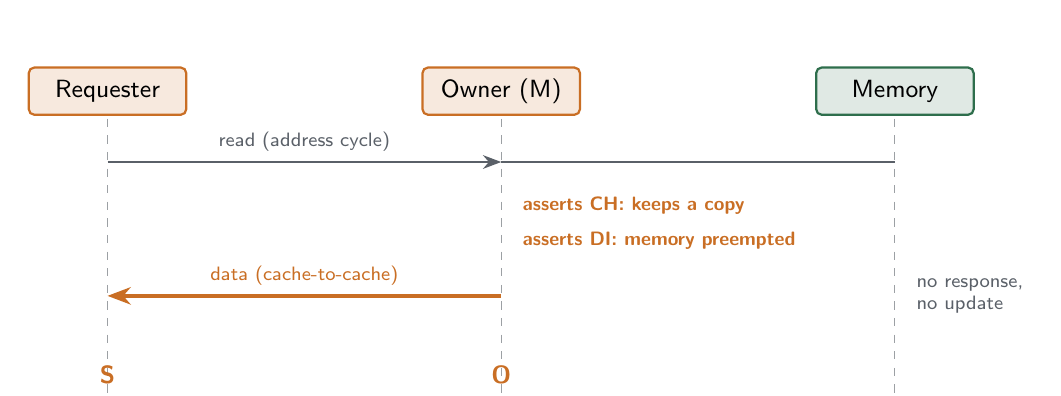
\begin{tikzpicture}[font=\sffamily\scriptsize,
    ag/.style={draw, thick, rounded corners=2pt, minimum width=2.0cm,
               minimum height=0.6cm, align=center, font=\sffamily\small},
    m/.style={-{Stealth}, thick}, sg/.style={font=\sffamily\bfseries\scriptsize}]
  \node[ag, fill=moesiOrange!15, draw=moesiOrange] (B) at (0,0) {Requester};
  \node[ag, fill=moesiOrange!15, draw=moesiOrange] (A) at (5.0,0) {Owner (\stM)};
  \node[ag, fill=memGreen!15, draw=memGreen] (Mm) at (10.0,0) {Memory};
  \foreach \x in {0,5,10} \draw[dashed, coreGrey!60] (\x,-0.35) -- (\x,-4.0);
  \draw[m, coreGrey] (0,-0.9) -- node[above]{read (address cycle)} (5,-0.9);
  \draw[coreGrey, thick] (5,-0.9) -- (10,-0.9);
  \node[sg, text=moesiOrange, anchor=west] at (5.15,-1.45) {asserts CH: keeps a copy};
  \node[sg, text=moesiOrange, anchor=west] at (5.15,-1.9) {asserts DI: memory preempted};
  \draw[m, moesiOrange, very thick] (5,-2.6) -- node[above]{data (cache-to-cache)} (0,-2.6);
  \node[text=coreGrey, align=left, anchor=west] at (10.15,-2.6) {no response,\\no update};
  \node[font=\sffamily\bfseries\small, text=moesiOrange] at (0,-3.6) {\stS};
  \node[font=\sffamily\bfseries\small, text=moesiOrange] at (5,-3.6) {\stO};
\end{tikzpicture}
\end{bigfig}
\caption[The \stM$\to$\stO\ transaction on Futurebus]{A remote read of a modified
line in a MOESI-class protocol, with the Futurebus signals of Sweazey and
Smith~\cite[pp.~417--418]{sweazey1986moesi}. The owner keeps the line and the
responsibility; memory neither responds nor is updated.}
\label{fig:futurebus-read}
\end{figure}

\begin{table}[htbp]
\centering
\caption{The \stO\ state, transaction by transaction.}
\label{tab:o-state-questions}
\small
\begin{tabular}{@{}L{4.0cm} L{8.9cm}@{}}
\toprule
Question & Answer and basis \\
\midrule
Why does the owner send the data? & Only the owner has the current value, and
  intervenient caches must supply it on a read miss~\cite[pp.~418--419]{sweazey1986moesi}. \\
Why \stO\ and not \stS? & \stS\ is unowned; moving to it would leave nobody
  responsible while memory is stale, breaking \cref{eq:owner-invariant}. \\
Why may memory stay stale? & The owner remains responsible and must update memory,
  pass ownership or answer for memory~\cite[p.~417]{sweazey1986moesi}. \\
Why can \stS\ coexist with \stO? & \stS\ copies are read-only and equal to the
  owner's; no copy can be written without first invalidating the others, so the
  order axiom holds. \\
Why is the owner still responsible? & Ownership is one of the three line
  attributes and is not given up by supplying data~\cite[p.~416]{sweazey1986moesi}. \\
What happens on eviction? & Copy-back: changes reach memory ``only when the line is
  replaced''~\cite[p.~416]{sweazey1986moesi}. \\
How are writes handled? & A write needs exclusiveness; the writer invalidates other
  copies (Futurebus \textsc{IM}, intent to modify) and holds the line in
  \stM~\cite[pp.~417--418]{sweazey1986moesi}. The old owner's data is superseded and
  is not written back. \\
\bottomrule
\end{tabular}
\end{table}

MESI and MOESI therefore differ in when memory is written; both are coherent. For a
producer and one consumer exchanging a block for $k$ rounds before it is evicted,
the memory writes over the block's lifetime are
\begin{equation}
  W_{\mathrm{MESI}}(k) = k,
  \qquad
  W_{\mathrm{MOESI}}(k) = 1,
  \label{eq:wb-timing}
\end{equation}
because MESI writes back at every \stM$\to$\stS\ transition and then evicts a clean
block, while MOESI writes back once, when the owner evicts. In the notation of
\cref{eq:fwb-fraction}, MOESI has $B_{\mathrm{fwb}}=0$ by construction. Its single
deferred writeback is a different quantity, $B_{\mathrm{dwb}}$, paid at eviction.
\Cref{eq:wb-timing} is our own count under the assumptions of Part~II.

In hardware, the \stO\ state needs three bits per line instead of
two~\cite[p.~416]{sweazey1986moesi}, and the bus must let a cache take over from
memory (\textsc{DI}) and announce that it keeps a copy (\textsc{CH}). Sweazey and
Smith also point out that Futurebus ``has no mechanism by which a transfer from one
cache to another can also update main memory''. Protocols that need that update,
including Write-Once and Firefly, have to abort the transaction with \textsc{BS}
(busy), write the line back and start again~\cite[p.~418]{sweazey1986moesi}. On
such a bus a MESI-style forced writeback costs an aborted and restarted
transaction, which is more than one extra transfer.

% ---------------------------------------------------------------
\section{Comparison and Limitations of Owner-Based Approaches}
\label{sec:own-compare}
\label{sec:own-limits}
\sectionmap{[Comparison and limits [Same ownership idea] [Berkeley lacks E]
  [Deferred not eliminated] [Implementations differ] [Benefit depends on workload]]}
\index{MESI}\index{MOESI}\index{MESIF}\index{Owned state}\index{Exclusive state}\index{forced writeback}\index{directory protocol}\index{Berkeley protocol}\index{Illinois protocol}\index{Futurebus}\index{gem5}\index{owner}%

Berkeley and MOESI use the same mechanism: on a remote read the owner supplies the
data, keeps ownership in a shared-dirty state, and leaves memory stale until
replacement. They differ in three ways. Berkeley has no \stE, so the first write
to a block fetched from memory costs a bus invalidation. Berkeley is one protocol
built for one controller, while MOESI is a class whose members may choose
different allowed actions. And the Futurebus version defines the bus signals
(\textsc{CH}, \textsc{DI}) that assert ownership. \Cref{tab:ownership-protocols}
adds the other published protocols with a shared-dirty state.

\begin{table}[htbp]
\centering
\caption{Table A: ownership-based protocols and shared-dirty variants.}
\label{tab:ownership-protocols}
\scriptsize
\begin{tabular}{@{}L{1.55cm} L{2.0cm} L{2.15cm} L{1.9cm} L{2.4cm} L{2.4cm}@{}}
\toprule
Protocol & State representation & Owner on remote read & Memory updated &
  Additional messages / signals & Principal limitation \\
\midrule
Berkeley~\cite{archibald1986evaluation} & \textsc{I, Valid, SD, Dirty};
  2 bits & supplies; \textsc{Dirty}/\textsc{SD}$\to$\textsc{SD}; requester
  \textsc{Valid} & on replacement of \textsc{SD} or \textsc{Dirty} &
  invalidation before any write to \textsc{Valid} or \textsc{SD} & no \stE:
  invalidation on first write even if unshared \\
MOESI class~\cite{sweazey1986moesi} & M, O, E, S, I; 3 bits & supplies
  (intervention); $\stM\to\stO$ & on replacement, or ownership passed &
  \textsc{CH}, \textsc{DI} bus signals & members may choose different
  actions; Futurebus cannot update memory during a transfer \\
Dragon~\cite{archibald1986evaluation} & \textsc{VE, SC, SD, Dirty};
  no invalid state & supplies; $\to$\textsc{SD}; requester \textsc{SC} &
  on replacement of \textsc{SD} & a bus update on every write to a shared
  block & update traffic per write (Chapter~12) \\
MESIF variant FM~\cite{goodman2009mesif} & proposed sixth state,
  Shared-Modified & requester may hold FM and defer cleansing & deferred;
  not specified & not specified & described in one paragraph only \\
MOESI-prime~\cite{loughlin2022moesiprime} & MOESI + M$'$, O$'$; 7 states,
  3 bits & as MOESI & as MOESI & avoids redundant in-DRAM directory writes
  & added directory-cache contention \\
\bottomrule
\end{tabular}
\end{table}

Owner-based protocols remove the forced writeback, but the memory update still has
to happen, and the literature gives no grounds for treating them as always better
than MESI. Five limits stand out.

\paragraph{The writeback is deferred.} The owner still writes the block back when
it evicts it (\cref{eq:wb-timing}). The saving is the $k-1$ overwritten writebacks
of \cref{sec:dirty-wasted}. If a block is shared once and then evicted, both
protocols make the same single write at different times. Whether the later write
is cheaper depends on when eviction happens; we pose this as RQ4 (\cref{tab:rq}),
and none of the sources answers it.

\paragraph{Memory is stale while an owner exists.} Every request for the block must
be answered by the owner, which must stand in for memory when
responding~\cite[p.~417]{sweazey1986moesi}. In our analysis this puts every read
of a widely shared dirty block on one cache's port, where MESI would let later
readers be served by memory or any sharer.

\paragraph{More state and control.} MOESI needs three bits per line instead of
two~\cite[p.~416]{sweazey1986moesi} and a bus that can preempt memory. The Berkeley
design needed explicit work on controller critical sections and
interlocks~\cite{katz1984implementing}, since races appear when ownership moves
during concurrent requests.

\paragraph{Implementations differ.} A protocol called MOESI need not perform the
\stM$\to$\stO\ transition. Mallya et al.\ report that the gem5
\texttt{MOESI\_CMP\_directory} implementation they used invalidates its copy on a
forwarded read of an \stM\ block instead of sharing dirty data, and that it differs
from \texttt{MESI\_Two\_Level} in many other states and
transitions~\cite{mallya2015simulation}. A ``MOESI versus MESI'' result has to be
read with the implementation in mind.

\paragraph{The benefit depends on the workload.} Every source that compares an
owner protocol with an invalidate protocol finds the advantage conditional.
Archibald and Baer report that Berkeley ``actually surpasses the Illinois scheme
at levels of high sharing'', because on a miss to a modified block Berkeley ``does
not require updating main memory as does
Illinois''~\cite[p.~295]{archibald1986evaluation}. Fagundes and Souza find that
MOESI's advantage over MESI shrinks as the LLC grows~\cite{fagundes2024evaluation}.
Loughlin et al.\ find that replacing MESI with their owner-based MOESI-prime cuts
the peak DRAM row activation rate substantially while changing execution time by
only $-0.51\,\%$ to $+0.61\,\%$~\cite{loughlin2022moesiprime}, so fewer memory
writes need not mean a shorter run.

\begin{remarkbox}[A note on sources]
We identified the original Berkeley report~\cite{katz1984implementing} and
paper~\cite{katz1985implementing} and checked their bibliographic details, but
could not read their full text. The state names and transitions above therefore
follow Archibald and Baer~\cite{archibald1986evaluation}. Other sources say the
original paper uses the terms UnOwned, Owned Exclusively and Owned NonExclusively;
we have not been able to check this against it.
\end{remarkbox}

% ===============================================================
%  Chapter 12 -- Other Extensions: MESIF and Write-Update Protocols
% ===============================================================
\chapter{Other Extensions: MESIF and Write-Update Protocols}
\label{ch:other-ext}
\index{MESIF}%

\begin{figure}[htbp]
\centering
\adjustbox{max width=\linewidth}{%
\begin{forest}
  chapter map,
  [Chapter 12
    [Write-update protocols [Firefly: caches and memory] [Dragon: caches only]
      [Update vs invalidate traffic]]
    [MESIF [The F state] [Reads of M lines migrate]]
    [Discussion [Remote-read decision tree] [Table B]]
  ]
\end{forest}}
\caption[]{Structure of Chapter~12. Neither family was
designed to remove the forced writeback; we look at what each does to it as a side
effect.}
\label{fig:ch12-map}
\end{figure}

% ---------------------------------------------------------------
\section{Write-Update Protocols}
\label{sec:ext-update}
\sectionmap{[Write-update [Writes propagate to sharers] [Firefly: also to memory]
  [Dragon: caches only with an owner] [Trade: no misses for update traffic]]}
\index{MESI}\index{MOESI}\index{forced writeback}\index{write-back cache}\index{write-through cache}\index{Berkeley protocol}\index{Dragon protocol}\index{Firefly protocol}\index{owner}%

A \gls{update} protocol keeps every cached copy valid by sending each write to the
other caches that hold the block (\cref{sec:coh-update-invalidate}). Archibald and
Baer call this the distributed-write approach and found that in their model it
``yields the best performance in the handling of shared
data''~\cite[p.~294]{archibald1986evaluation}. Firefly and Dragon are often
grouped together, but they update memory and assign ownership differently, and
that difference decides what each does to the forced writeback.

\paragraph{Firefly.} The DEC Firefly cache has two tag bits per line,
\textsc{Dirty} and \textsc{Shared}, and the bus has a signal, \textsc{MShared},
``asserted during an operation if another cache contains the requested
location''~\cite[p.~7]{thacker1987firefly}. A write to an unshared line is handled
as in any write-back cache and ``requires no MBus traffic''. A shared line is
written through: ``the cache does write-through, and other caches that share the
datum are updated, as is main storage''~\cite[p.~7]{thacker1987firefly}. On a read
miss, when another cache holds the line, ``the caches that contain the line supply
the data, and the memory is inhibited''~\cite[p.~8]{thacker1987firefly}. If the
supplying cache holds the line dirty, Archibald and Baer say the block is supplied
and ``written to main memory at the same time'', after which every cache holding
it, the requester included, is in \textsc{Shared}~\cite[p.~280]{archibald1986evaluation}.
Firefly therefore never lets a modified block be shared. On the transaction of
\cref{fig:dirty-transaction} it makes the same memory update as MESI, and after
that every write to the shared block also goes to memory: ``the Firefly must send
distributed writes to memory while the Dragon sends them to the caches
only''~\cite[p.~295]{archibald1986evaluation}. Firefly keeps the forced writeback
and adds a memory write for each later shared write.

\paragraph{Dragon.} Dragon's states are \textsc{Valid-Exclusive},
\textsc{Shared-Clean}, \textsc{Shared-Dirty} and \textsc{Dirty}, with no invalid
state~\cite{archibald1986evaluation}. On a read miss to a block held elsewhere in
\textsc{Dirty} or \textsc{Shared-Dirty}, the holder ``supplies the data, raises the
SharedLine, and sets its block state to \textsc{Shared-Dirty}'', and the requester
takes the block as \textsc{Shared-Clean}~\cite[p.~281]{archibald1986evaluation}.
Writes to a shared block are broadcast to the other holders, and ``the single-word
write does not go to main memory''~\cite[p.~282]{archibald1986evaluation}. ``The
last cache to write it, if any, will have the block in state \textsc{Shared-Dirty}''
and is ``responsible for updating memory when the block is
replaced''~\cite[p.~281]{archibald1986evaluation}. Dragon thus has the same
ownership idea as Berkeley and MOESI, a single shared-dirty owner responsible for
memory, combined with update in place of invalidation, and on a remote read of a
modified block it defers the writeback as MOESI does. Sweazey and Smith place
Dragon in the MOESI class and note that its memory is updated ``only on a
replacement''~\cite[p.~420]{sweazey1986moesi}.

\paragraph{Update traffic against forced writebacks.} Without invalidations there
are no misses after a write, but each write to a shared block costs a bus
transaction, so the outcome depends on how many writes the producer makes between
reads. We add one assumption to the counting rules of \cref{tab:msg-classes}: a
single-word update is an 8-byte header plus an 8-byte word, $u=16$\,B. For one
producer, $C$ consumers and $w$ producer writes per round, the steady-state bytes
per round are
\begin{align}
  B_{\mathrm{MESI}}(C)            &= 160 + 80\,(C-1), \label{eq:upd-mesi}\\
  B_{\mathrm{MOESI}}(C)           &= \phantom{1}88 + 80\,(C-1), \label{eq:upd-moesi}\\
  B_{\mathrm{Dragon}}(w)          &= B_{\mathrm{Firefly}}(w) = u\,w = 16\,w. \label{eq:upd-dragon}
\end{align}
\Cref{eq:upd-mesi} is \cref{eq:pc-model}. In \cref{eq:upd-moesi} the owner serves
the consumer's read without a writeback ($8+72$\,B) and the producer's write is an
invalidating upgrade (8\,B). In \cref{eq:upd-dragon} the consumers' reads all hit
and one bus update reaches every sharer, so the cost does not depend on $C$.
Firefly sends the same bus bytes, but each of its $w$ updates also writes memory.
These are our analytical counts. \Cref{fig:update-vs-invalidate} explains how two
observations that seem to clash can both hold. Archibald and Baer, whose synthetic
workload made single-word references to shared blocks, found distributed write
best for shared data~\cite[p.~294]{archibald1986evaluation}, and Chapter~4 gave the
usual argument that invalidation wins when a core writes a block many times before
others read it. The two results sit on opposite sides of the crossover.

\begin{figure}[htbp]
\centering
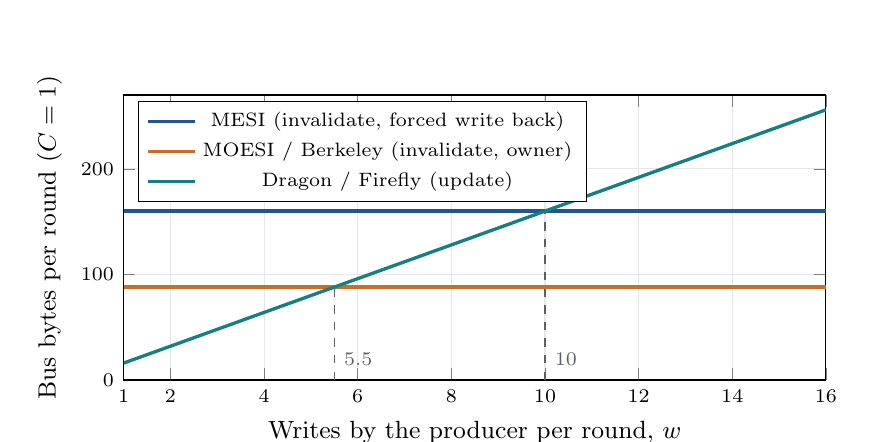
\begin{tikzpicture}
  \begin{axis}[width=10.5cm, height=5.2cm,
      xlabel={Writes by the producer per round, $w$},
      ylabel={Bus bytes per round ($C=1$)},
      xmin=1, xmax=16, ymin=0, ymax=270, xtick={1,2,4,6,8,10,12,14,16},
      legend style={at={(0.02,0.98)}, anchor=north west, font=\scriptsize},
      grid=major, grid style={coreGrey!15},
      label style={font=\small}, tick label style={font=\scriptsize}]
    \addplot[very thick, mesiBlue, domain=1:16] {160};
    \addlegendentry{MESI (invalidate, forced write back)}
    \addplot[very thick, moesiOrange, domain=1:16] {88};
    \addlegendentry{MOESI / Berkeley (invalidate, owner)}
    \addplot[very thick, tealC, domain=1:16] {16*x};
    \addlegendentry{Dragon / Firefly (update)}
    \draw[dashed, coreGrey] (axis cs:5.5,0) -- (axis cs:5.5,88);
    \draw[dashed, coreGrey] (axis cs:10,0) -- (axis cs:10,160);
    \node[font=\scriptsize, text=coreGrey, anchor=south west] at (axis cs:5.5,4) {5.5};
    \node[font=\scriptsize, text=coreGrey, anchor=south west] at (axis cs:10,4) {10};
  \end{axis}
\end{tikzpicture}
\caption[Update and invalidate traffic per producer--consumer round]{Bus bytes per
round for one producer and one consumer
(\cref{eq:upd-mesi,eq:upd-moesi,eq:upd-dragon}). Update protocols move fewer bytes
than MESI below ten writes per round and fewer than MOESI below 5.5; above those
points invalidation is cheaper. Firefly also writes memory once per update. Our
analytical model.}
\label{fig:update-vs-invalidate}
\end{figure}

% ---------------------------------------------------------------
\section{MESIF: The Forward State}
\label{sec:ext-mesif}
\sectionmap{[MESIF [Point-to-point interconnect] [F: one clean forwarder]
  [A read of M migrates the line] [F is not O]]}
\index{MOESI}\index{MESIF}\index{forced writeback}\index{snooping protocol}\index{directory protocol}\index{sharing patterns!producer--consumer}%

Goodman and Hum describe \gls{mesif}, finished in 2001 and used in Intel's
QuickPath Interconnect, as a way to get the latency of snooping on a point-to-point
network~\cite[\S1]{goodman2009mesif}. Their reference point is a directory
protocol, which needs ``a minimum of three serial communications to complete a
memory transaction'' where snooping needs two~\cite[\S1]{goodman2009mesif}. When
several caches hold a clean line in \stS, none of them is named to answer, so the
home memory has to serve the request. The Forward state is ``a state assigned to a
single node among those sharing a cache line'', and that node is ``responsible for
providing its content when a request is received''~\cite[\S2.1]{goodman2009mesif}.
When the F holder answers a read, the requester gets the line in F and the old
holder drops to \stS~\cite[\S2.1.1, case ii]{goodman2009mesif}, so the role moves to
the latest reader. The authors compare F to an owned state, ``but coherent with
memory and useful for read requests rather than write
requests''~\cite[\S2.1]{goodman2009mesif}.

The report treats a read of a line that another node holds in \stM\ as its hardest
case. In the basic protocol ``the line is transmitted to the requesting node as if
the request had been a Read-for-Ownership'': the holder gives up its copy and the
requester gets the line exclusively~\cite[\S2.1.1, case iv]{goodman2009mesif}. No
memory update is described for this case. A variant lets the holder keep a copy in
\stS; the requester must then either ``cleanse'' the line, meaning write it back,
or keep it in a sixth state, Shared-Modified (FM), which postpones the write. The
report says nothing more about FM~\cite[\S2.1.1, case iv]{goodman2009mesif}.

The basic behaviour avoids the forced writeback by another route than MOESI:
modified data is never shared because the line migrates. In a producer--consumer
exchange this costs something MOESI does not pay. By our analysis the producer
loses its copy at every consumer read, so its next write is a miss that must fetch
the data (an 8-byte request and a 72-byte transfer) instead of an 8-byte upgrade,
and with $C$ consumers the line migrates on every read. The paper's projected gain
of 6 to 11\,\% for four nodes comes from an in-house mean-value-analysis model whose
algorithms, the authors say, ``cannot be divulged''~\cite[\S3]{goodman2009mesif}.
For the hitI and hitS cases ``MESIF offers no benefits over the 3-hop
protocols''~\cite[\S3]{goodman2009mesif}. The protocol adds snoop stalls while a
forwarding node waits for an acknowledgement, needs the home node to identify every
party to a conflict ``even in the case of read-only (shared) data'', and uses three
virtual channels per direction to avoid deadlock~\cite[\S2.1--2.3]{goodman2009mesif}.
\Cref{tab:f-vs-o} sets F against O.

\begin{table}[htbp]
\centering
\caption{The Forward state and the Owned state compared.}
\label{tab:f-vs-o}
\small
\begin{tabular}{@{}L{3.6cm} L{4.3cm} L{4.3cm}@{}}
\toprule
 & F (MESIF) & O (MOESI) \\
\midrule
Data relative to memory & clean: ``coherent with memory''~\cite[\S2.1]{goodman2009mesif}
  & dirty: memory may be stale~\cite[p.~416]{sweazey1986moesi} \\
Responsible for write back & no & yes \\
Purpose & choose one cache to answer reads of clean shared data &
  let modified data be shared without updating memory \\
Effect on the forced writeback & none; the \stM\ case is handled by
  migration & removes it; deferred to eviction \\
Interconnect assumed & point-to-point with a home node & designed for a
  shared bus (Futurebus) \\
\bottomrule
\end{tabular}
\end{table}

% ---------------------------------------------------------------
\section{Limitations and Discussion}
\label{sec:ext-discussion}
\sectionmap{[Discussion [Five answers to one transaction] [Update: trades misses for writes]
  [Forwarding: a latency fix] [Table B]]}
\index{Dragon protocol}\index{Firefly protocol}%

\Cref{fig:remote-read-tree} sorts the protocols of Chapters~11 and~12 by what they
do on the one transaction this report studies. The sources show five different
behaviours, and only one of them both shares the data and leaves the holder
responsible for it. Write-update and forwarding target other costs than the one in
Chapter~10. Update protocols remove the misses caused by invalidation and pay with
a bus transaction per shared write (\cref{fig:update-vs-invalidate}); Dragon also
defers memory updates through ownership and Firefly does not. Forwarding reduces
the latency of serving clean shared data on a point-to-point network, and handles
modified data by migration at the cost of the producer's copy.
\Cref{tab:alt-strategies} summarises the three.

\begin{figure}[htbp]
\centering
\adjustbox{max width=0.9\linewidth}{%
\begin{forest}
  decision tree,
  [Remote read of a modified block:\\does the holder supply the data?
    [{Synapse: holder sends NAK\\writes back; requester\\retries from memory}, el=no]
    [Does the holder\\keep a copy?, el=yes
      [{MESIF (basic): line\\migrates as a\\read-for-ownership}, el=no]
      [Is memory updated\\at this point?, el=yes
        [{Illinois / MESI\\Write-once, Firefly:\\forced write back}, el=yes]
        [{Berkeley, MOESI\\Dragon: holder stays\\responsible owner}, el=no]]]]
\end{forest}}
\caption[Decision tree: remote read of a modified block]{Five published behaviours
on the transaction studied here. Synapse, Write-once, Illinois, Firefly, Berkeley
and Dragon from Archibald and Baer~\cite[pp.~276--281]{archibald1986evaluation};
MESIF from Goodman and Hum~\cite[\S2.1.1]{goodman2009mesif}; MOESI from Sweazey and
Smith~\cite[pp.~416--419]{sweazey1986moesi}.}
\label{fig:remote-read-tree}
\end{figure}

\begin{table}[htbp]
\centering
\caption{Table B: alternative coherence strategies and the forced writeback.}
\label{tab:alt-strategies}
\scriptsize
\begin{tabular}{@{}L{1.3cm} L{1.7cm} L{2.3cm} L{2.3cm} L{2.0cm} L{2.6cm}@{}}
\toprule
Protocol & Strategy & State or forwarding mechanism & Shared modified data &
  Memory updated & Relevance to the forced writeback \\
\midrule
Firefly & update, write-through when shared & \textsc{Dirty} and
  \textsc{Shared} tag bits; \textsc{MShared} line~\cite{thacker1987firefly} &
  not allowed; dirty block written to memory when supplied~\cite{archibald1986evaluation}
  & on every shared write and on eviction & retains it, and adds a memory
  write per shared write \\
Dragon & update, caches only & \textsc{VE, SC, SD, Dirty};
  \textsc{SD} owner~\cite{archibald1986evaluation} & allowed (\textsc{SD})
  & on replacement of \textsc{SD}~\cite{archibald1986evaluation} & removes it
  (defers), but adds an update per shared write \\
MESIF & invalidate, clean forwarding & F: one forwarder among clean
  copies~\cite{goodman2009mesif} & not in the basic protocol; FM variant
  proposed & not stated for the basic \stM\ case & addresses a related
  problem; avoids it by migration in the basic protocol \\
\bottomrule
\end{tabular}
\end{table}

% ===============================================================
%  Chapter 13 -- Scaling Approaches: Directories and Token Coherence
% ===============================================================
\chapter{Scaling Approaches: Directories and Token Coherence}
\label{ch:scaling-approaches}

\begin{figure}[htbp]
\centering
\adjustbox{max width=\linewidth}{%
\begin{forest}
  chapter map,
  [Chapter 13
    [Directories [DASH protocol] [Sharing write back] [Owner-retaining variant]]
    [Token coherence [Counting tokens] [Owner token] [Persistent requests]]
    [Discussion [Organisation vs semantics] [Table C]]
  ]
\end{forest}}
\caption[]{Structure of Chapter~13. Both approaches change
how coherence messages travel and are ordered; the block-state rules on top
decide what happens to the dirty-sharing transaction.}
\label{fig:ch13-map}
\end{figure}

% ---------------------------------------------------------------
\section{Directory-Based Coherence}
\label{sec:scal-dir}
\sectionmap{[Directories [Replace broadcast by a sharer list] [DASH: three directory states]
  [Remote dirty read: four messages] [Memory is updated: sharing write back]]}
\index{MESI}\index{MOESI}\index{Owned state}\index{dirty sharing}\index{snooping protocol}\index{directory protocol}\index{DASH}\index{owner}%

Chapter~8 showed that snoop lookups grow as $N(N-1)$ (\cref{eq:snoop}) and that a
bus saturates once demand passes its capacity (\cref{eq:util}). A
\gls{directory}\index{directory protocol} replaces broadcast with a per-block record
of the caches that may hold the block, so requests reach only those
caches~\cite{censier1978directory}. A directory decides where a request goes and
where it is ordered. Whether a modified block may be shared is a separate
question, decided by the state protocol.

The Stanford DASH multiprocessor is the standard published example of a directory
protocol for distributed shared memory. Each memory block is uncached-remote,
shared-remote or dirty-remote in the directory, and each cached copy is invalid,
shared or dirty~\cite[\S4]{lenoski1990dash}. A directory entry has one state bit and
a bit vector with ``a bit for each of the sixteen clusters
supported''~\cite[\S3]{lenoski1990dash}, which by our count is 17 bits per memory
block. A request that reaches a cluster no longer holding the block gets a negative
acknowledgement and is sent again~\cite[\S4.1, \S4.6]{lenoski1990dash}.

The transaction of interest is a read of a block that is dirty in a remote cluster.
The home directory forwards the request ``to the owning, dirty cluster''. The owner
sends the data straight to the requester and also sends a sharing writeback to the
home: ``The sharing writeback request writes the cache block back to memory and
also updates the directory.'' The directory entry becomes shared-remote and the old
owner's copy becomes read-only~\cite[\S4.1]{lenoski1990dash}. The paper gives no
reason for updating memory at this point. This three-cluster transaction takes
about 80 processor clocks, against about 61 for a read served by a remote home with
no dirty copy~\cite[\S4.2, Fig.~6]{lenoski1990dash}. DASH thus performs, through
the home node and over a network, the same memory update that MESI performs on a
bus. Its cache states have no shared-dirty state, so a dirty block must become
clean when it is shared, and moving from snooping to a directory changes only the
route the transaction takes.

A directory can keep a dirty owner if it records which cache is the owner as well
as the sharers. A read of a dirty block is then forwarded to the owner, answered
from its cache and logged as a new sharer, with no writeback. Loughlin et al.\
study this combination on Intel's directory-based ccNUMA systems. They show that
MESI's ``downgrade writebacks'' on dirty sharing reach DRAM, that MOESI's \stO\
state removes them, and their MOESI-prime adds two states to avoid redundant
writes of the in-DRAM directory as well~\cite{loughlin2022moesiprime}.
\Cref{fig:dir-dirty-read} compares DASH with an owner-retaining directory. The
second is our construction, assuming one control message tells the home about the
new sharer.

\begin{figure}[htbp]
\centering
\begin{bigfig}[0.88]
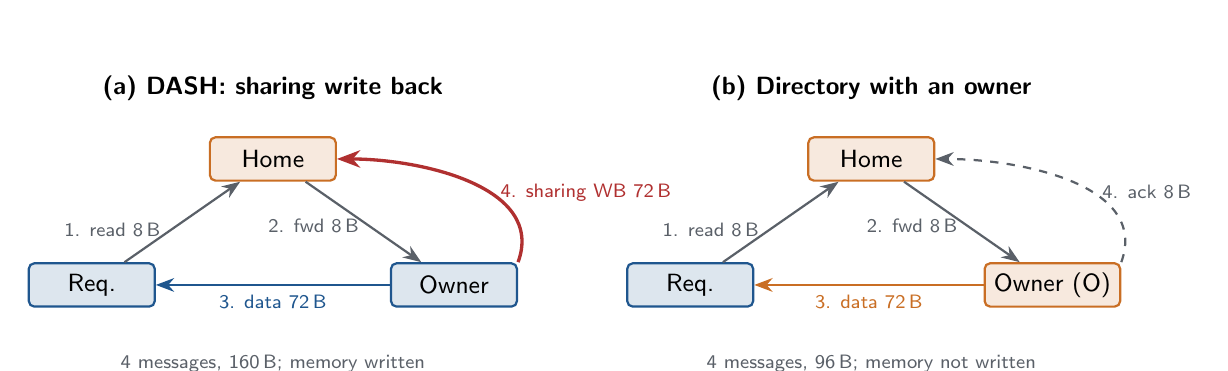
\begin{tikzpicture}[font=\sffamily\scriptsize,
    ag/.style={draw, thick, rounded corners=2pt, minimum width=1.6cm,
               minimum height=0.55cm, font=\sffamily\small, align=center},
    m/.style={-{Stealth}, thick}]
  \node[font=\sffamily\bfseries\small] at (2.3,2.5) {(a) DASH: sharing write back};
  \node[ag, fill=mesiBlue!15, draw=mesiBlue] (R) at (0,0) {Req.};
  \node[ag, fill=moesiOrange!15, draw=moesiOrange] (H) at (2.3,1.6) {Home};
  \node[ag, fill=mesiBlue!15, draw=mesiBlue] (O) at (4.6,0) {Owner};
  \draw[m, coreGrey] (R) -- node[left, pos=0.4]{1. read 8\,B} (H);
  \draw[m, coreGrey] (H) -- node[left, pos=0.55]{2. fwd 8\,B} (O);
  \draw[m, mesiBlue] (O) -- node[below]{3. data 72\,B} (R);
  \draw[m, alertRed, very thick] (O.north east) to[out=70, in=0] node[right, text=alertRed, pos=0.4]{4. sharing WB 72\,B} (H.east);
  \node[text=coreGrey] at (2.3,-1.0) {4 messages, 160\,B; memory written};
  \begin{scope}[xshift=7.6cm]
  \node[font=\sffamily\bfseries\small] at (2.3,2.5) {(b) Directory with an owner};
  \node[ag, fill=mesiBlue!15, draw=mesiBlue] (R2) at (0,0) {Req.};
  \node[ag, fill=moesiOrange!15, draw=moesiOrange] (H2) at (2.3,1.6) {Home};
  \node[ag, fill=moesiOrange!15, draw=moesiOrange] (O2) at (4.6,0) {Owner (\stO)};
  \draw[m, coreGrey] (R2) -- node[left, pos=0.4]{1. read 8\,B} (H2);
  \draw[m, coreGrey] (H2) -- node[left, pos=0.55]{2. fwd 8\,B} (O2);
  \draw[m, moesiOrange] (O2) -- node[below]{3. data 72\,B} (R2);
  \draw[m, coreGrey, dashed] (O2.north east) to[out=70, in=0] node[right, pos=0.4]{4. ack 8\,B} (H2.east);
  \node[text=coreGrey] at (2.3,-1.0) {4 messages, 96\,B; memory not written};
  \end{scope}
\end{tikzpicture}
\end{bigfig}
\caption[A remote dirty read under two directory protocols]{A read of a block dirty
in another cache. (a)~DASH~\cite[\S4.1]{lenoski1990dash}: the sharing writeback
updates memory and the directory. (b)~An owner-retaining directory (our
construction): a control message records the new sharer and memory stays stale.
Both have three messages on the critical path; bytes use \cref{tab:msg-classes}.}
\label{fig:dir-dirty-read}
\end{figure}

% ---------------------------------------------------------------
\section{Token Coherence}
\label{sec:scal-token}
\sectionmap{[Token coherence [T tokens per block] [One token to read; all to write]
  [The owner token carries data] [Correctness substrate plus performance policy]]}
\index{MOESI}\index{directory protocol}\index{token coherence}\index{write-invalidate}\index{sharing patterns!migratory}\index{owner}\index{reading indices}%

Martin, Hill and Wood separate the mechanism that keeps a system correct from the
one that makes it fast~\cite{martin2003token}. The correctness substrate counts
tokens\index{token coherence}: ``the system assigns each block $T$ tokens (where $T$
is at least as large as the number of processors)'', and a processor ``can write a
block only if it holds all $T$ tokens'' and ``can read a block only if it holds at
least one token''~\cite[\S3.1]{martin2003token}. A writer must collect every token,
so nobody else can hold a readable copy during a write. This gives the
single-writer property of write-invalidate without an ordered interconnect.

One token is the owner token, and ``if a coherence message contains the owner
token, it must contain data''. Holding the owner token without all the others
``maps to the familiar MOESI state owned (O)''~\cite[\S3.1]{martin2003token}. On a
shared (read) request, a holder missing some tokens ``sends the data with one token
(usually not the owner token)''~\cite[\S4.2]{martin2003token}. On eviction a
processor returns all its tokens to memory, with data if the owner token is among
them~\cite[\S3.1]{martin2003token}. The paper does not state directly what happens
to memory on a read of a modified block. From these rules we infer that the owner
keeps the owner token and the duty to return data to memory, so the read is served
without a memory update, as in MOESI. One exception is stated: a processor that has
all tokens and has written the block answers a shared request with ``the data and
all tokens''~\cite[\S4.2]{martin2003token}, an optimisation for migratory sharing
that hands over ownership instead of sharing it.

Requests in the performance policy are ``fast, unordered `hint' requests'' that may
fail. A processor that suspects starvation issues a persistent request, and the
substrate activates ``at most one persistent request per
block''~\cite[\S3.2, \S4.1]{martin2003token}. The evaluated policy, TokenB,
broadcasts all transient requests over an unordered two-dimensional
torus~\cite[\S4.2, \S5.2]{martin2003token}. On a simulated 16-processor SPARC system
running OLTP, Apache and SPECjbb, ``only 3.0\,\% of cache misses are issued more
than once and only 0.2\,\% resort to persistent requests''. TokenB is reported
17--54\,\% faster than the paper's directory protocol and 8--29\,\% faster than its
Hammer protocol, while the directory protocol ``uses 21--25\,\% less'' interconnect
traffic~\cite[\S6]{martin2003token}. Token state costs $2+\log_2 T$ bits per block,
one byte for $T=64$ with 64-byte blocks~\cite[\S3.1]{martin2003token}.

TokenB removes the indirection of \cref{fig:dir-dirty-read}, since the owner answers
the requester directly, and by the inference above it also removes the writeback.
It pays with broadcast. Counting each broadcast as $N-1$ point-to-point messages of
8 bytes (the paper's request size~\cite[\S5.1]{martin2003token}), a read served by
an owner costs
\begin{equation}
  B_{\mathrm{TokenB}}(N) = 8\,(N-1) + 72 \ \text{bytes},
  \label{eq:tokenb}
\end{equation}
or 80, 96, 128 and 192 bytes for 2, 4, 8 and 16 processors. This is our analytical
count; the paper reports aggregate traffic, not this transaction.

% ---------------------------------------------------------------
\section{Limitations and Discussion}
\label{sec:scal-discussion}
\sectionmap{[Discussion [Directories cut broadcast and add a hop]
  [Tokens cut the hop and add broadcast] [Writeback set by the state rules] [Table C]]}
\index{MOESI}\index{directory protocol}\index{token coherence}\index{DASH}\index{owner}%

Directories and tokens answer the scaling problem of Chapter~8 in opposite ways. A
directory removes broadcast but adds an indirection and per-block storage that
grows with the processor count; Lenoski et al.\ note that full bit vectors grow with
both memory size and processor count and suggest limited-pointer and sparse
directories~\cite[\S6]{lenoski1990dash}. Token coherence removes the indirection and
needs no ordered interconnect, but uses broadcast requests and a starvation
mechanism. Neither, by its organisation alone, decides whether a modified block is
written back when shared. DASH writes it back, while an owner-retaining directory,
MOESI-prime and the owner token do not (\cref{tab:organisations}). Reducing
communication overhead and removing premature writebacks are therefore independent
goals, and published systems combine either kind of organisation with either kind
of state protocol.

\begin{table}[htbp]
\centering
\caption{Table C: coherence organisations, separating communication and
permissions from the dirty-sharing transaction.}
\label{tab:organisations}
\scriptsize
\begin{tabular}{@{}L{1.55cm} L{2.2cm} L{1.9cm} L{2.0cm} L{2.0cm} L{2.6cm}@{}}
\toprule
Organisation & Communication & Ordering point & Permission mechanism &
  Extra storage & Dirty-sharing transaction \\
\midrule
Snooping bus & broadcast to all caches & the bus & block states (MSI family)
  & none & set by the state protocol: MESI writes back, MOESI defers \\
Directory (DASH) & point-to-point via home & home directory & directory
  state + cache states & state bit + sharer vector per block~\cite{lenoski1990dash}
  & DASH writes back (sharing writeback)~\cite{lenoski1990dash}; an
  owner-retaining directory need not~\cite{loughlin2022moesiprime} \\
Token (TokenB) & broadcast hints, unordered torus & none needed; persistent
  requests for starvation & token counts and owner token & $2+\log_2T$ bits
  per block~\cite{martin2003token} & owner token keeps responsibility; no
  memory update inferred~\cite{martin2003token} \\
\bottomrule
\end{tabular}
\end{table}

% ===============================================================
%  Chapter 14 -- Comparative Analysis of Existing Solutions
% ===============================================================
\chapter{Comparative Analysis of Existing Solutions}
\label{ch:comparative}

\begin{figure}[htbp]
\centering
\adjustbox{max width=\linewidth}{%
\begin{forest}
  chapter map,
  [Chapter 14
    [Mechanisms [Three classes] [Nine approaches]]
    [Traffic [Counting rules] [Four sharing patterns]]
    [Trade-offs {\&} evaluations [{Latency, state}] [Seven studies]]
    [Research gap [Table D] [Two open questions]]
  ]
\end{forest}}
\caption[]{Structure of Chapter~14: one set of criteria, from
Chapter~10, applied to every approach of Chapters~11 to~13.}
\label{fig:ch14-map}
\end{figure}

% ---------------------------------------------------------------
\section{Comparison of Underlying Mechanisms}
\label{sec:cmp-mechanisms}
\sectionmap{[Mechanisms [Direct solutions change the states]
  [Alternative strategies change propagation] [Organisations change communication]
  [Nine approaches in one table]]}
\index{Dragon protocol}%

\Cref{fig:classes} places each approach in one of the three classes of Part~III.
Dragon appears twice because it combines an ownership state with update.
\Cref{tab:mechanisms} records, for each approach, the properties that decide its
behaviour on the transaction of \cref{fig:dirty-transaction}. The last two rows are
organisations, not complete state protocols, so their entries describe the
published protocols evaluated with them.

\begin{figure}[htbp]
\centering
\adjustbox{max width=0.82\linewidth}{%
\begin{forest}
  for tree={
    grow'=0, parent anchor=east, child anchor=west, anchor=west,
    align=center, font=\sffamily\small, draw, thick, rounded corners=3pt,
    inner sep=4pt, l sep+=14pt, s sep+=1pt,
    edge={thick, coreGrey!60, -{Stealth[length=5pt]}},
  },
  [Approaches\\reviewed, fill=mesiBlue, draw=mesiBlue, text=white, font=\sffamily\bfseries\small
    [Direct solutions:\\shared-dirty owner, fill=memGreen!20, draw=memGreen
      [Berkeley, fill=memGreen!8, draw=memGreen!60]
      [MOESI class, fill=memGreen!8, draw=memGreen!60]
      [Dragon (owner part), fill=memGreen!8, draw=memGreen!60]]
    [Alternative strategies:\\propagation and forwarding, fill=moesiOrange!20, draw=moesiOrange
      [Firefly: update and write-through, fill=moesiOrange!8, draw=moesiOrange!60]
      [Dragon (update part), fill=moesiOrange!8, draw=moesiOrange!60]
      [MESIF: clean forwarding, fill=moesiOrange!8, draw=moesiOrange!60]]
    [Organisations:\\how requests travel, fill=coreGrey!20, draw=coreGrey
      [Directory (DASH), fill=coreGrey!8, draw=coreGrey!60]
      [Token coherence, fill=coreGrey!8, draw=coreGrey!60]]
  ]
\end{forest}}
\caption[Classification of the approaches reviewed]{The three classes. Only the
first targets the forced writeback by design; the second affects it as a side
effect; the third leaves it to the state protocol on top.}
\label{fig:classes}
\end{figure}

\begin{table}[htbp]
\centering
\caption{Underlying mechanisms of the approaches reviewed. ``WB'' = writeback.}
\label{tab:mechanisms}
\scriptsize
\begin{tabular}{@{}L{1.25cm} L{1.35cm} L{1.75cm} L{1.05cm} L{1.05cm} L{1.75cm} L{1.85cm} L{1.75cm}@{}}
\toprule
Approach & Strategy & State or permission model & Dirty data shared? &
  Explicit owner? & Supplier on remote read & Memory updated & Forced WB \\
\midrule
MSI & invalidate & M, S, I~\cite{sarangi2025basic} & no & M only & holder of M &
  at M$\to$S and on eviction of M & present \\
MESI & invalidate & M, E, S, I~\cite{papamarcos1984illinois} & no & M only & holder of M &
  at M$\to$S and on eviction of M & present (baseline) \\
MOESI & invalidate & M, O, E, S, I~\cite{sweazey1986moesi} & yes (O) & yes &
  owner (M or O) & on eviction of owner & eliminated; deferred to eviction \\
Berkeley & invalidate & I, Valid, SD, Dirty~\cite{archibald1986evaluation} & yes (SD)
  & yes & owner & on eviction of owner & eliminated; deferred to eviction \\
Dragon & update & VE, SC, SD, Dirty~\cite{archibald1986evaluation} & yes (SD)
  & yes & owner & on eviction of SD owner & eliminated; replaced by update traffic \\
Firefly & update, write-through & Dirty, Shared bits~\cite{thacker1987firefly} &
  no & no & caches holding it & at sharing, on every shared write, on eviction & retained; extra memory writes \\
MESIF & invalidate, forwarding & M, E, S, I, F~\cite{goodman2009mesif} & no (basic)
  & no & F holder (clean); M holder by migration & not stated for the M case &
  avoided by migration (basic) \\
Directory (DASH) & organisation & 3 directory + 3 cache states~\cite{lenoski1990dash}
  & no & dirty owner only & owner, forwarded by home & sharing WB at the remote read &
  retained \\
Token (TokenB) & organisation & token counts, owner token~\cite{martin2003token}
  & yes (owner token) & yes & owner-token holder & on eviction of owner token &
  eliminated (inferred) \\
\bottomrule
\end{tabular}
\end{table}

% ---------------------------------------------------------------
\section{Comparison of Communication and Memory Traffic}
\label{sec:cmp-traffic}
\sectionmap{[Traffic [One set of counting rules] [Bus protocols in one table]
  [Point-to-point counted separately] [Bar graphs per pattern]]}
\index{MESI}\index{MOESI}\index{MESIF}\index{Exclusive state}\index{directory protocol}\index{token coherence}\index{Dragon protocol}\index{sharing patterns!producer--consumer}\index{sharing patterns!migratory}\index{owner}%

None of the sources reports traffic for these protocols in one common
configuration, so this section is our own analytical accounting. It applies the
rules of \cref{tab:counting-rules} to the same access sequences under each
protocol. Bus and point-to-point protocols are counted separately, since one bus
broadcast and $N-1$ point-to-point messages are different costs.

\begin{table}[htbp]
\centering
\caption{Counting rules for the analytical comparison. Rows~1--3 are those of
\cref{tab:msg-classes}; rows~4--6 are assumptions added for Part~III.}
\label{tab:counting-rules}
\small
\begin{tabular}{@{}c L{5.4cm} L{6.0cm}@{}}
\toprule
 & Item & Rule \\
\midrule
1 & Control message (request, invalidation, upgrade) & 8\,B on the interconnect \\
2 & Data message (block to a cache) & 72\,B (64\,B block + 8\,B header) \\
3 & Writeback message & 72\,B on the interconnect; 64\,B written to memory \\
4 & Word update (Dragon, Firefly) & 16\,B (8\,B header + 8\,B word); Firefly
  also writes 8\,B to memory \\
5 & Bus broadcast & counted once: one transaction reaches all caches \\
6 & Point-to-point broadcast (TokenB) & counted as $N-1$ messages \\
\bottomrule
\end{tabular}
\end{table}

\Cref{tab:traffic-patterns} gives the cost of each sharing pattern of
\cref{tab:patterns} under the six bus protocols, as interconnect bytes and bytes
written to memory, derived from the transitions cited in Chapters~11 and~12. A
migratory hand-off under MESI, for example, is a read miss served by the \stM\
holder with a writeback ($8+72+72$) followed by an upgrade (8), 160\,B in all.
Under MOESI the owner serves the read without a writeback ($8+72$) and the upgrade
invalidates the old owner, whose data is superseded (8), giving 88\,B. Under
Dragon every core keeps a copy once it has taken part, so in steady state a
hand-off is one update; the writer becomes \textsc{Shared-Dirty} and the previous
owner \textsc{Shared-Clean}~\cite[p.~282]{archibald1986evaluation}.

\begin{table}[htbp]
\centering
\caption{Analytical traffic per unit of each sharing pattern, as interconnect
bytes\,/\,bytes written to memory, with one producer write per round ($w=1$) and
one consumer ($C=1$). Our counts, using \cref{tab:counting-rules}.}
\label{tab:traffic-patterns}
\small
\begin{tabular}{@{}L{3.0cm} c c c c c c@{}}
\toprule
Pattern (unit) & MSI & MESI & MOESI & Berkeley & Dragon & Firefly \\
\midrule
Private (read, write, evict) & 160\,/\,64 & 152\,/\,64 & 152\,/\,64 & 160\,/\,64 & 152\,/\,64 & 152\,/\,64 \\
Read-only (per reader) & 80\,/\,0 & 80\,/\,0 & 80\,/\,0 & 80\,/\,0 & 80\,/\,0 & 80\,/\,0 \\
Producer--consumer (per round) & 160\,/\,64 & 160\,/\,64 & 88\,/\,0$^{*}$ & 88\,/\,0$^{*}$ & 16\,/\,0$^{*}$ & 16\,/\,8 \\
Migratory (per hand-off) & 160\,/\,64 & 160\,/\,64 & 88\,/\,0$^{*}$ & 88\,/\,0$^{*}$ & 16\,/\,0$^{*}$ & 16\,/\,8 \\
\bottomrule
\multicolumn{7}{@{}p{12.6cm}@{}}{\footnotesize $^{*}$Plus one deferred
writeback (72\,B, 64\,B to memory) when the owner finally evicts the block,
amortised over all rounds. Private-pattern differences come only from the
\stE\ state: MSI and Berkeley need an upgrade on the first write; the others
upgrade silently~\cite[pp.~279--282]{archibald1986evaluation}.}
\end{tabular}
\end{table}

The private and read-only patterns cost the same under every protocol apart from
the \stE\ effect, so a workload made of them gains nothing from ownership or
update. In producer--consumer and migratory sharing, ownership removes every
memory write and cuts interconnect bytes by 45\,\% relative to MESI, which is the
forced-writeback fraction of \cref{eq:pc-model}. Update protocols move the fewest
bytes at $w=1$, but lose that advantage as $w$ grows
(\cref{fig:update-vs-invalidate}). \Cref{fig:bars-pc,fig:bars-mig} show the two
patterns in which the protocols differ.

\begin{figure}[htbp]
\centering
\begin{minipage}[t]{0.5\linewidth}\centering
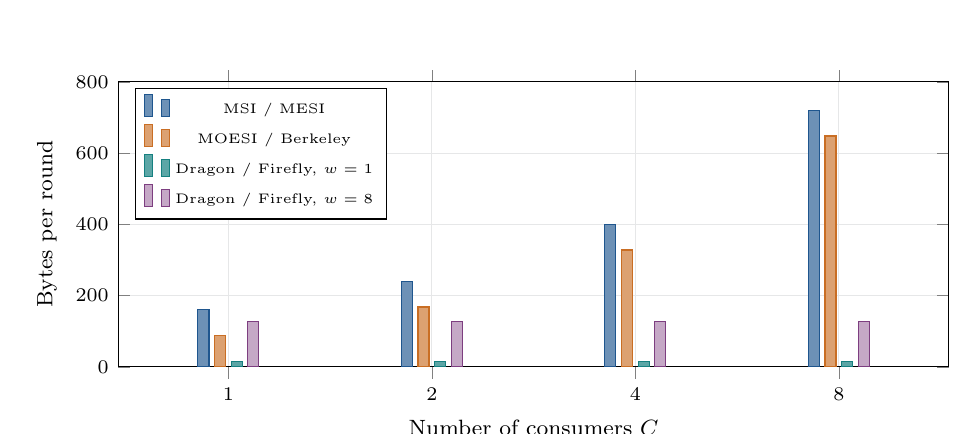
\begin{tikzpicture}
  \begin{axis}[width=\linewidth, height=5.2cm, ybar, bar width=4pt,
      xlabel={Number of consumers $C$}, ylabel={Bytes per round},
      symbolic x coords={1,2,4,8}, xtick=data, ymin=0, ymax=800,
      enlarge x limits=0.18,
      legend style={at={(0.02,0.98)}, anchor=north west, font=\tiny},
      grid=major, grid style={coreGrey!15},
      label style={font=\footnotesize}, tick label style={font=\scriptsize}]
    \addplot[fill=mesiBlue!65, draw=mesiBlue] coordinates {(1,160) (2,240) (4,400) (8,720)};
    \addlegendentry{MSI / MESI}
    \addplot[fill=moesiOrange!65, draw=moesiOrange] coordinates {(1,88) (2,168) (4,328) (8,648)};
    \addlegendentry{MOESI / Berkeley}
    \addplot[fill=tealC!70, draw=tealC] coordinates {(1,16) (2,16) (4,16) (8,16)};
    \addlegendentry{Dragon / Firefly, $w=1$}
    \addplot[fill=plumC!45, draw=plumC] coordinates {(1,128) (2,128) (4,128) (8,128)};
    \addlegendentry{Dragon / Firefly, $w=8$}
  \end{axis}
\end{tikzpicture}
\caption[Producer--consumer traffic by protocol]{Producer--consumer: ownership saves
72 bytes per round; update cost does not depend on $C$ but grows with $w$. Firefly
also writes $8w$ bytes to memory. Our model.}
\label{fig:bars-pc}
\end{minipage}\hfill
\begin{minipage}[t]{0.48\linewidth}\centering
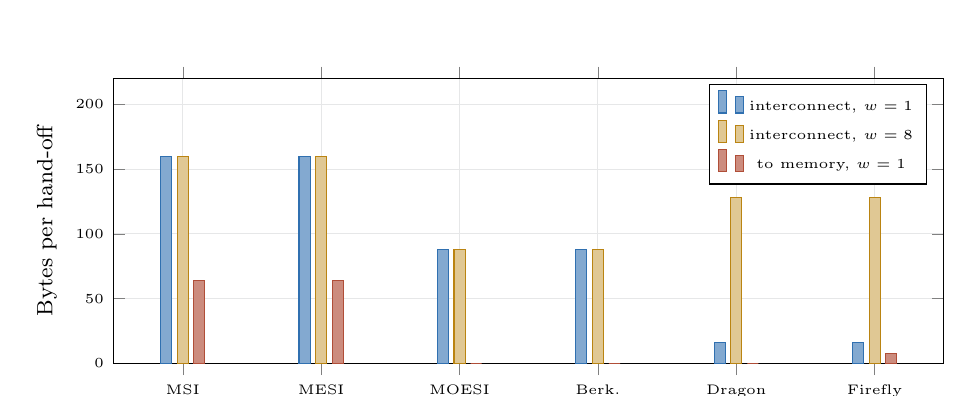
\begin{tikzpicture}
  \begin{axis}[width=\linewidth, height=5.2cm, ybar, bar width=4pt,
      ylabel={Bytes per hand-off},
      symbolic x coords={MSI,MESI,MOESI,Berk.,Dragon,Firefly}, xtick=data,
      ymin=0, ymax=220, enlarge x limits=0.1,
      legend style={at={(0.98,0.98)}, anchor=north east, font=\tiny},
      grid=major, grid style={coreGrey!15},
      label style={font=\footnotesize}, tick label style={font=\tiny}]
    \addplot[fill=skyC!60, draw=skyC] coordinates
      {(MSI,160) (MESI,160) (MOESI,88) (Berk.,88) (Dragon,16) (Firefly,16)};
    \addlegendentry{interconnect, $w=1$}
    \addplot[fill=amberC!45, draw=amberC] coordinates
      {(MSI,160) (MESI,160) (MOESI,88) (Berk.,88) (Dragon,128) (Firefly,128)};
    \addlegendentry{interconnect, $w=8$}
    \addplot[fill=brickC!65, draw=brickC] coordinates
      {(MSI,64) (MESI,64) (MOESI,0) (Berk.,0) (Dragon,0) (Firefly,8)};
    \addlegendentry{to memory, $w=1$}
  \end{axis}
\end{tikzpicture}
\caption[Migratory-sharing traffic by protocol]{Migratory: bytes per hand-off when
each core reads a block and writes it $w$ times. Only MSI and MESI write memory at
every hand-off. Our model.}
\label{fig:bars-mig}
\end{minipage}
\end{figure}

For the point-to-point organisations of Chapter~13 the dirty-sharing transaction is
compared in \cref{tab:p2p}. Removing the writeback saves the same 64 bytes of memory
traffic in the directory and token organisations, while TokenB's interconnect cost
grows with $N$ and the directory's does not. We do not cost MESIF: its message set
(invalid-state acknowledgements, cancellations and data acknowledgements to the
home node~\cite[\S2.1.1]{goodman2009mesif}) belongs to a protocol the report gives
only in outline, and a byte count would rest on assumptions the source does not
support.

\begin{table}[htbp]
\centering
\caption{The remote dirty read on point-to-point organisations. Our analytical
counts, using \cref{tab:counting-rules}.}
\label{tab:p2p}
\small
\begin{tabular}{@{}L{3.9cm} c c c c@{}}
\toprule
Organisation & Messages & Bytes & Critical-path hops & Memory written \\
\midrule
Directory, DASH (sharing WB)~\cite{lenoski1990dash} & 4 & 160 & 3 & 64\,B \\
Directory with owner (\cref{fig:dir-dirty-read}b) & 4 & 96 & 3 & 0 \\
TokenB, $N=4$ (\cref{eq:tokenb}) & 4 & 96 & 2 & 0 \\
TokenB, $N=16$ (\cref{eq:tokenb}) & 16 & 192 & 2 & 0 \\
\bottomrule
\end{tabular}
\end{table}

% ---------------------------------------------------------------
\section{Trade-offs and Published Evaluations}
\label{sec:cmp-tradeoffs}
\label{sec:cmp-evaluations}
\sectionmap{[Trade-offs [Latency evidence from the papers] [State and storage cost]
  [Fewer write backs need not mean less time] [Seven studies]]}
\index{MESI}\index{MOESI}\index{MESIF}\index{Exclusive state}\index{forced writeback}\index{token coherence}\index{Berkeley protocol}\index{Dragon protocol}\index{Firefly protocol}\index{Illinois protocol}\index{Futurebus}\index{DASH}\index{gem5}\index{cache-to-cache transfer}%

The sources report latency in different units and configurations, so only
comparisons within one study mean anything. On Futurebus a protocol that must
update memory during a cache-to-cache transfer aborts and restarts the
transaction~\cite[p.~418]{sweazey1986moesi}, so the forced writeback lengthens the
read itself. In DASH a read involving a dirty remote cluster takes about 80
processor clocks against about 61 for a clean remote
read~\cite[\S4.2, Fig.~6]{lenoski1990dash}. MESIF cuts a read of a line held in E, M
or F to two hops but offers ``no benefits over the 3-hop protocols'' for lines in I
or S~\cite[\S3]{goodman2009mesif}. TokenB answers in two hops but reissues 3.0\,\%
of misses~\cite[\S6]{martin2003token}. The state and storage costs are in row~10 of
\cref{tab:matrix}: three bits per line plus the \textsc{DI} and \textsc{CH} signals
for MOESI~\cite[p.~416]{sweazey1986moesi}, a 17-bit entry per block for 16-cluster
DASH~\cite[\S3]{lenoski1990dash}, and $2+\log_2T$ bits plus a persistent-request table of 8 bytes per arbiter
for tokens~\cite[\S3.1--3.2]{martin2003token}.

Removing a memory writeback does not by itself reduce total traffic or execution
time. The saved bytes can be replaced by update traffic (Dragon), kept alongside it
(Firefly) or traded for broadcast requests (TokenB), and saved traffic becomes
saved time only when the interconnect or memory was the bottleneck
(\cref{fig:bus-util}). MOESI-prime is the clearest published case: it removed MESI's
downgrade writebacks and reached its goal of fewer DRAM row activations, while
execution time changed by between $-0.51\,\%$ and
$+0.61\,\%$~\cite{loughlin2022moesiprime}.

\Cref{tab:evaluations} lists the comparative studies we found. Their set-ups range
from a synthetic single-bus model and queueing analysis to full-system simulation of
commercial workloads and gem5 runs with different protocol implementations, so
their numbers cannot be compared with each other and we do not compare them.
Stenstr{\"o}m~\cite{stenstrom1990survey} surveys hardware and software coherence
schemes of the same period. Two points matter for this report. The only early study
that compared an ownership protocol with an invalidate protocol under identical
conditions, Archibald and Baer, compared whole protocols: Berkeley and Illinois
differ both in having \stE\ and in ownership (\cref{tab:berkeley-states}), so the
effect of ownership alone cannot be read from their
results~\cite{archibald1986evaluation}. And the recent gem5 studies compare
implementations that differ in many ways; in the case reported by Mallya et al.\
the MOESI implementation did not share dirty data on our
transaction~\cite{mallya2015simulation}.

\begin{table}[htbp]
\centering
\caption{Published comparative evaluations relevant to the forced writeback.}
\label{tab:evaluations}
\scriptsize
\begin{tabular}{@{}L{1.75cm} L{2.0cm} L{2.0cm} L{2.15cm} L{2.6cm} L{2.0cm}@{}}
\toprule
Study & Protocols & Method and system & Workload, metric & Principal finding &
  Isolates the O state? \\
\midrule
Archibald {\&} Baer 1986~\cite{archibald1986evaluation} & Write-once, Synapse,
  Berkeley, Illinois, Firefly, Dragon & simulation; one bus; 1--15 processors &
  synthetic streams; ``system power'' & update best for shared data; Berkeley
  beats Illinois at high sharing (p.~295) & no: whole protocols differ \\
Yang et al.\ 1989~\cite{yang1989analysis} & the six above and write-through &
  queueing model (MVA); packet-switched bus & analytical & full text not
  consulted & --- \\
Martin et al.\ 2003~\cite{martin2003token} & TokenB, snooping, directory,
  Hammer & Simics full system; 16 processors & OLTP, Apache, SPECjbb; runtime,
  traffic & TokenB faster; directory 21--25\,\% less traffic & no: organisations
  compared \\
Goodman {\&} Hum 2009~\cite{goodman2009mesif} & MESIF vs.\ 3-hop & in-house MVA,
  undisclosed & projection & 6--11\,\% (4 nodes) & no \\
Mallya et al.\ 2015~\cite{mallya2015simulation} & MI, MESI, MOESI & gem5 Ruby;
  2--4 nodes & SPLASH-2; misses, energy & MESI better in some cases & no:
  different gem5 protocols \\
Loughlin et al.\ 2022~\cite{loughlin2022moesiprime} & MESI, MOESI, MOESI-prime &
  gem5; 2--8 nodes & PARSEC, SPLASH-2x; row activations & MOESI removes downgrade
  writebacks; runtime within $\pm0.61\,\%$ & not established \\
Fagundes {\&} Souza 2024~\cite{fagundes2024evaluation} & MESI, MOESI & gem5 full
  system; 4, 8 cores & one OpenMP kernel ($\pi$) & MOESI better, less so with
  larger L2 & no \\
\bottomrule
\end{tabular}
\end{table}

% ---------------------------------------------------------------
\section{Research Gap and Motivation for Our Contribution}
\label{sec:cmp-gap}
\sectionmap{[Gap [What the literature establishes] [Table D]
  [Open 1: isolate the O state] [Open 2: predict the benefit]]}
\index{MESI}\index{MOESI}\index{Owned state}\index{sharing patterns!migratory}\index{gem5}%

The sources establish four points. Ownership protocols let modified data be shared
without updating memory and stay coherent~\cite{sweazey1986moesi,archibald1986evaluation},
so the timing of the memory update is a design choice. Different approaches trade
memory traffic, interconnect traffic and hardware state against one another
(\cref{tab:traffic-patterns,tab:p2p}). And the benefit of each depends on the
workload's sharing
behaviour~\cite[p.~295]{archibald1986evaluation}\cite{fagundes2024evaluation,loughlin2022moesiprime}.
\Cref{tab:matrix} judges every approach against the requirements of Chapter~10.

\begin{table}[htbp]
\centering
\caption{Table D: every approach against the requirements of Chapter~10.
DA: directly addresses; PA: partially addresses; RP: addresses a related
problem; OR: orthogonal; NE: not established by the available source.}
\label{tab:matrix}
\scriptsize
\begin{tabular}{@{}L{2.05cm} L{1.4cm} L{1.4cm} L{1.4cm} L{1.4cm} L{1.4cm} L{1.4cm} L{1.4cm}@{}}
\toprule
Criterion & MOESI & Berkeley & Dragon & Firefly & MESIF & Directory (DASH) & Token \\
\midrule
1 Completion & yes$^{a}$ & yes$^{a}$ & yes$^{a}$ & yes$^{a}$ & yes$^{a}$ & yes$^{a}$ & yes$^{a}$ \\
2 Order & yes$^{a}$ & yes$^{a}$ & yes$^{a}$ & yes$^{a}$ & yes$^{a}$ & yes$^{a}$ & yes$^{a}$ \\
3 Removes the immediate forced WB & DA: deferred & DA: deferred & DA: deferred &
  no: retained & PA: by migration & no: sharing WB & DA (inferred) \\
4 Keeps silent E$\to$M & yes & no: no E & yes (VE) & yes (VE) & E present; NE &
  OR: no E state & NE \\
5 Shares modified data & yes & yes & yes & no & no; FM proposed & no & yes \\
6 Explicit ownership & yes & yes & yes & no & no & dirty owner only & yes \\
7 Extra control traffic & none over MESI & invalidation on first write &
  update per shared write & update per shared write & home acks (IACK, CNCL,
  DACK) & forward + acks & broadcast; 3\,\% reissue \\
8 Extra data traffic & none & none & none & none & producer re-fetch (our
  analysis) & sharing WB & none (inferred) \\
9 Memory bandwidth & lower & lower & lower & higher & NE & as MESI & lower
  (inferred) \\
10 Hardware & 3 bits; DI, CH & 2 bits; interlocks & update path & update path;
  MShared & 3 bits; 3 VCs & 17 bits per block & $2+\log_2T$ bits \\
11 Scalability & bus-based as published & bus-based & bus-based & bus-based &
  point-to-point & scalable & unordered; broadcast \\
12 Workload sensitivity & high-sharing gains & high-sharing gains & writes per
  read & writes per read & E, M, F hits only & NE & commercial only \\
\bottomrule
\multicolumn{8}{@{}p{12.6cm}@{}}{\footnotesize $^{a}$As published; each
protocol is presented by its authors as coherent. Formal verification is
outside the scope of this report (\cref{sec:prob-scope}).}
\end{tabular}
\end{table}

Two questions remain open, and Part~IV takes them up.

\paragraph{Isolating the effect of the Owned state.} None of the studies in
\cref{tab:evaluations} compares MESI and MOESI with \stO\ as the only difference.
The early comparison varied whole protocols, and the gem5 comparisons used
implementations that differ in many states and transitions, in one case without
the \stM$\to$\stO\ transition at all. We do not claim that no such study exists
anywhere, only that the studies we found do not provide one, so their results
cannot be credited to the \stO\ state alone. Part~IV therefore builds a controlled
simulator in which MESI and MOESI share every component and setting, leaving the
\stM$\to$\stO\ behaviour as the single changed variable.

\paragraph{Predicting the benefit from MESI behaviour.} The sources agree that the
benefit of ownership depends on sharing, and Archibald and Baer parameterise their
model by the fraction of references to shared
blocks~\cite[p.~286]{archibald1986evaluation}. Detecting sharing patterns is also
known: adaptive protocols classify blocks as migratory at run time and change how
they handle them~\cite{stenstrom1993adaptive}, using rules such as spotting a write
by a processor other than the last writer~\cite{nilsson1994adaptive}. We did not
find a workload measure, taken under MESI, that has been proposed and tested as a
predictor of the gain from moving to MOESI. Part~IV defines the Dirty Sharing
Ratio, the fraction of coherence transactions in which a read is served by a cache
holding the block in \stM, for this purpose. It differs from adaptive detection in
being an offline characterisation used to choose a protocol, rather than a run-time
mechanism inside one.

% ===============================================================
%  PART IV -- Our Contribution (Chapters 15--16)
%  Method and analysis only. Results are in Part VI; the simulator
%  is described in Part V. Proofs are in Appendix D (rule 7).
% ===============================================================

\newtheorem{proposition}{Proposition}[chapter]

\part{Our Contribution}
\label{part:contribution}

\begin{center}
\adjustbox{max width=\linewidth}{%
\begin{forest}
  part map,
  [Part IV
    [Ch.~15: A Controlled Method
      [One changed variable] [Everything else held fixed] [Paired runs] [Correctness first]]
    [Ch.~16: The Dirty Sharing Ratio
      [One counter under MESI] [Dirty epochs] [An exact saving identity] [From bytes to time] [Hypotheses H1--H4]]
  ]
\end{forest}}
\end{center}

\begin{keybox}[What Part IV does]
Part~III left two open questions (\cref{sec:cmp-gap}): none of the studies we
found isolates the effect of the \stO\ state, and none offers a workload measure,
taken under MESI, that predicts the gain from moving to MOESI. Chapter~15 answers
the first with a controlled comparison in which \stO\ is the only difference
between the two protocols. Chapter~16 answers the second with the Dirty Sharing
Ratio and derives an exact identity linking it to the traffic MOESI saves. Four
hypotheses, one per research question, close the Part. Everything here is derived
from the counting rules of \cref{tab:counting-rules}; no result depends on a
simulation.
\end{keybox}

% ===============================================================
%  Chapter 15 -- A Controlled Method for Isolating the Owned State
% ===============================================================
\chapter{A Controlled Method for Isolating the Owned State}
\label{ch:method}

\begin{figure}[htbp]
\centering
\adjustbox{max width=\linewidth}{%
\begin{forest}
  chapter map,
  [Chapter 15
    [Why comparisons mislead [Whole protocols differ] [Confounders]]
    [The one changed variable [Three rules differ] [Diff of the FSMs]]
    [Held fixed {\&} paired [Controlled variables] [Same trace twice]]
    [Same cache contents [Proposition 15.1] [Worked example]]
    [Correctness first [Invariants] [Version numbers]]
  ]
\end{forest}}
\caption[]{Structure of Chapter~15: why existing
comparisons cannot isolate the \stO\ state, the single change the method makes,
what it holds fixed, and how the runs are checked.}
\label{fig:ch15-map}
\end{figure}

% ---------------------------------------------------------------
\section{Why Existing Comparisons Cannot Isolate the Owned State}
\label{sec:method-why}
\sectionmap{[The difficulty [A protocol is many decisions] [Implementations differ in all of them]
  [A measured gap has many causes] [We need one variable]]}
\index{MESI}\index{MOESI}\index{Owned state}\index{coherence axioms}%

A coherence protocol is made of many decisions: which states exist, who supplies
data on a miss, when memory is updated, whether a clean block may be forwarded
between caches, how races are resolved and how each message is timed. Two
published implementations called ``MESI'' and ``MOESI'' differ in many of these at
once. Chapter~14 showed this for the evaluations we reviewed
(\cref{tab:evaluations}): the early study compared whole protocols, and the
simulator studies used implementations that differ in several states and
transitions, in one case without the \stM$\to$\stO\ transition at all. When such a
study reports that MOESI is faster, the gap could come from \stO, from a better
forwarding policy, from a different cache set-up, or from all of these.
\Cref{fig:method-idea} contrasts that kind of comparison with ours. Our method
removes each of these sources of difference: MOESI is MESI plus \stO\ with every
other rule identical (\cref{sec:method-delta}), both runs share one cache model, bus
and set of message sizes and replay the same trace (\cref{sec:method-fixed}),
differences are taken per trace before averaging over seeds, and both coherence
axioms are checked on every access so that a bug cannot pass for a speed-up
(\cref{sec:method-correct}).

\begin{figure}[htbp]
\centering
\begin{bigfig}[0.95]
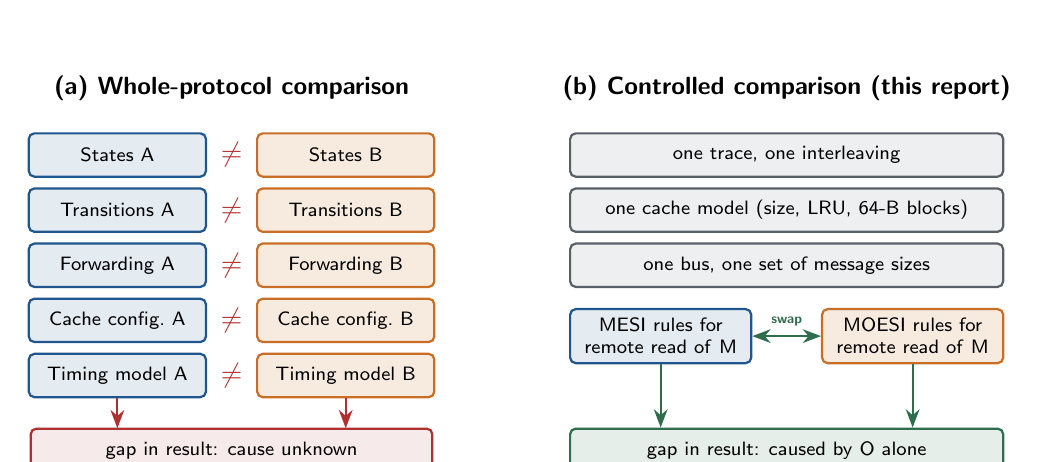
\begin{tikzpicture}[font=\sffamily\scriptsize,
    bx/.style={draw, thick, rounded corners=2pt, minimum width=2.15cm, minimum height=0.55cm, align=center},
    ar/.style={-{Stealth}, thick}]
  \node[font=\sffamily\bfseries\small] at (2.6,4.65) {(a) Whole-protocol comparison};
  \foreach \y/\t in {3.8/States, 3.1/Transitions, 2.4/Forwarding, 1.7/Cache config., 1.0/Timing model} {
    \node[bx, fill=mesiBlue!12, draw=mesiBlue, minimum width=2.25cm] at (1.15,\y) {\t\ A};
    \node[bx, fill=moesiOrange!14, draw=moesiOrange, minimum width=2.25cm] at (4.05,\y) {\t\ B};
    \node[text=alertRed, font=\sffamily\bfseries] at (2.6,\y) {$\neq$};
  }
  \node[bx, fill=alertRed!10, draw=alertRed, minimum width=5.1cm] (ra) at (2.6,0.05) {gap in result: cause unknown};
  \draw[ar, alertRed] (1.15,0.72) -- (1.15,0.33); \draw[ar, alertRed] (4.05,0.72) -- (4.05,0.33);
  \begin{scope}[xshift=6.9cm]
  \node[font=\sffamily\bfseries\small] at (2.75,4.65) {(b) Controlled comparison (this report)};
  \node[bx, fill=coreGrey!10, draw=coreGrey, minimum width=5.5cm] at (2.75,3.8) {one trace, one interleaving};
  \node[bx, fill=coreGrey!10, draw=coreGrey, minimum width=5.5cm] at (2.75,3.1) {one cache model (size, LRU, 64-B blocks)};
  \node[bx, fill=coreGrey!10, draw=coreGrey, minimum width=5.5cm] at (2.75,2.4) {one bus, one set of message sizes};
  \node[bx, fill=mesiBlue!12, draw=mesiBlue, minimum width=2.3cm] (tm) at (1.15,1.5) {MESI rules for\\remote read of \stM};
  \node[bx, fill=moesiOrange!14, draw=moesiOrange, minimum width=2.3cm] (to) at (4.35,1.5) {MOESI rules for\\remote read of \stM};
  \draw[{Stealth}-{Stealth}, thick, memGreen] (tm.east) -- node[above, font=\sffamily\bfseries\tiny, text=memGreen]{swap} (to.west);
  \node[bx, fill=memGreen!12, draw=memGreen, minimum width=5.5cm] (rb) at (2.75,0.05) {gap in result: caused by \stO\ alone};
  \draw[ar, memGreen] (tm) -- (tm|-rb.north); \draw[ar, memGreen] (to) -- (to|-rb.north);
  \end{scope}
\end{tikzpicture}
\end{bigfig}
\caption[Whole-protocol versus controlled comparison]{(a) Comparing two separately
built protocols changes many things at once. (b) Our method runs one simulator
twice on the same input and changes only the rules that involve \stO.}
\label{fig:method-idea}
\end{figure}

% ---------------------------------------------------------------
\section{The One Changed Variable}
\label{sec:method-delta}
\sectionmap{[The delta [MOESI as MESI plus O] [Three rules change]
  [All other rules identical] [Written as a diff]]}
\index{MESI}\index{MOESI}\index{Owned state}\index{owner}%

MOESI is a class of protocols whose members may choose different allowed actions
(\cref{sec:own-moesi}), so a comparison has to fix one member. We take the member
closest to MESI: it adds \stO\ and changes only the three rules that \stO\ forces,
and is otherwise the MESI of \cref{fig:mesi}.
\begin{enumerate}[itemsep=1pt]
  \item Remote read of a block in \stM. MESI: the holder supplies the block,
    writes it back and moves to \stS. MOESI: the holder supplies the block without
    writing it back and moves to \stO.
  \item Remote read of a block in \stO\ (MOESI only): the owner supplies the block
    and stays in \stO; memory is not involved.
  \item Eviction of a block in \stO\ (MOESI only): the owner writes the block back,
    as an eviction from \stM\ does. \stS\ copies stay.
\end{enumerate}
A write by any cache to a block in \stO\ or \stS\ is an upgrade in both protocols:
one control message invalidates all other copies and the writer moves to \stM. If
the writer did not hold the block, the owner (in \stM\ or \stO) supplies it and is
invalidated, and memory is not written because the writer becomes the new dirty
owner. \Cref{fig:moesi-diff} draws the difference as a diff of the two state
machines and \cref{tab:transition-diff} lists every rule. Other members of the
class may also forward clean blocks or hand ownership to the latest reader, but
each of those is a second change. Leaving them out answers the narrow question of
what \stO\ itself does; such features could be added later and studied one at a
time with the same method.

\begin{figure}[htbp]
\centering
\begin{bigfig}[1.0]
\begin{tikzpicture}[fsm]
  \node[font=\sffamily\bfseries\small] at (2.5,4.5) {(a) MESI: remote read of \stM};
  \node[stB] (M) at (0,3.0) {\stM};
  \node[stB] (S) at (5.0,3.0) {\stS};
  \node[stB] (I) at (2.5,0.2) {\stI};
  \draw[key] (M) -- node[lb, above, text=alertRed]{readmiss / send data\\+ \textbf{write back}} (S);
  \draw[bus] (M) -- node[lb, left=3pt]{writemiss /\\send data} (I);
  \draw[bus] (S) -- node[lb, right=3pt]{write, writemiss /\\---} (I);
  \node[lb, text=coreGrey] at (2.5,1.95) {memory now up to date};
  \begin{scope}[xshift=7.6cm]
  \node[font=\sffamily\bfseries\small] at (2.5,4.5) {(b) MOESI: the same event};
  \node[stO] (M2) at (0,3.0) {\stM};
  \node[stO] (O2) at (5.0,3.0) {\stO};
  \node[stO] (I2) at (0,0.2) {\stI};
  \node[stO] (S2) at (5.0,0.2) {\stS};
  \draw[good] (M2) -- node[lb, above, text=memGreen]{readmiss / send data\\(no write back)} (O2);
  \draw[good] (O2) to[out=30, in=-30, looseness=7] node[lb, right]{readmiss /\\send data} (O2);
  \draw[bus] (M2) -- node[lb, left=3pt]{writemiss /\\send data} (I2);
  \draw[bus] (O2) to[bend right=12] node[lb, sloped, above, pos=0.42]{write, writemiss / send data if needed} (I2);
  \draw[tr] (O2) to[bend left=12] node[lb, sloped, below, pos=0.58]{evict / write back} (I2);
  \draw[bus] (S2) -- node[lb, below]{write, writemiss / ---} (I2);
  \end{scope}
\end{tikzpicture}
\end{bigfig}
\caption[MESI and MOESI as a diff]{The only transitions that differ between the
two protocols compared. (a) In MESI a remote read of a modified block forces a
writeback (red). (b) In MOESI the same event moves the holder to \stO\ without one
(green); the owner answers later reads and writes back only on eviction. All
other transitions are as in \cref{fig:mesi}.}
\label{fig:moesi-diff}
\end{figure}

\begin{table}[htbp]
\centering
\caption{Transition rules of the two protocols compared. Shaded rows are the only
ones that differ, so any measured difference between the runs comes from them.}
\label{tab:transition-diff}
\small
\begin{tabular}{@{}L{3.6cm} L{4.5cm} L{4.6cm}@{}}
\toprule
Event (state of other copies) & MESI & MOESI \\
\midrule
Read miss, no other copy & memory supplies; requester \stE & same \\
Read miss, copies in \stE/\stS & memory supplies; \stE$\to$\stS; requester \stS & same \\
\rowcolor{moesiOrange!12}
Read miss, a copy in \stM & holder supplies \textbf{and writes back}; holder \stS & holder supplies; holder \stO \\
\rowcolor{moesiOrange!12}
Read miss, a copy in \stO & (cannot occur) & owner supplies; owner stays \stO \\
Write hit in \stE / \stM & silent; requester \stM & same \\
Write hit in \stS (or \stO) & upgrade (8\,B) invalidates others; \stM & same \\
Write miss, a dirty copy exists & owner supplies; others invalidated; \stM & same \\
Write miss, no dirty copy & memory supplies; others invalidated; \stM & same \\
Evict \stS\ or \stE & silent & same \\
Evict \stM & write back (72\,B) & same \\
\rowcolor{moesiOrange!12}
Evict \stO & (cannot occur) & write back (72\,B) \\
\bottomrule
\end{tabular}
\end{table}

% ---------------------------------------------------------------
\section{What Is Held Fixed, and Paired Runs}
\label{sec:method-fixed}
\label{sec:method-paired}
\sectionmap{[Controlled variables [{Trace, caches, bus, latencies}] [Attribution test]
  [{One trace, two runs}] [Differences before averages]]}
\index{MESI}\index{MOESI}\index{Owned state}%

\Cref{tab:controlled} lists what is held constant and how the simulator of Part~V
enforces it. \Cref{fig:attribution-tree} turns the table into a test: a difference
between the two runs may be credited to \stO\ only if every question is answered
``yes''. The evaluations reviewed in Chapter~14 do not pass this test.

\begin{table}[htbp]
\centering
\caption{Controlled variables, identical in the MESI and MOESI runs of every
experiment.}
\label{tab:controlled}
\small
\begin{tabular}{@{}L{3.6cm} L{4.6cm} L{4.6cm}@{}}
\toprule
Variable & Value & Enforced by \\
\midrule
Memory-access trace & one list of (core, block, read/write) & generated once per seed, replayed twice \\
Order of accesses & trace order (traffic study); each core's own order (timing study) & one replay loop for both protocols \\
Cache per core & private, write-back, fully associative, LRU, 64-B blocks & one cache class; capacity a parameter \\
Interconnect & one snooping bus; broadcasts counted once & one bus model \\
Message sizes & 8\,B control, 72\,B data and writeback & constants of \cref{tab:counting-rules} \\
Latencies (timing study) & $T_{L1}$, $T_{\mathrm{mem}}$, $T_{\mathrm{coh}}$ of Chapters~2 and~8 & one parameter set per experiment \\
Accounting at the end & blocks still dirty are written back once & same drain step for both \\
\bottomrule
\end{tabular}
\end{table}

\begin{figure}[htbp]
\centering
\adjustbox{max width=0.95\linewidth}{%
\begin{forest}
  decision tree,
  [{Is the difference between\\the two runs caused by \stO?}
    [{Same trace and\\same interleaving?}
      [{Same caches, bus,\\message sizes, latencies?}, el=yes
        [{All rules not involving\\\stO\ identical?}, el=yes
          [{Both runs pass the\\coherence checks?}, el=yes
            [{Yes: attribute\\the difference to \stO}, el=yes]
            [{No: one run is wrong;\\fix before comparing}, el=no]]
          [{No: a second feature\\differs (not controlled)}, el=no]]
        [{No: configuration\\confounds the result}, el=no]]
      [{No: different sharing,\\not comparable}, el=no]]
  ]
\end{forest}}
\caption[Attribution test]{Decision tree for crediting a measured difference to
\stO. Each ``no'' leaf names the confounder that could explain the difference
instead.}
\label{fig:attribution-tree}
\end{figure}

Because one trace $W$ is replayed under both protocols, every configuration gives a
pair of results. For any quantity $X$ (bytes, writebacks, execution time) we
compute, per pair,
\begin{equation}
  \Delta X(W) = X(\mathrm{MESI},W) - X(\mathrm{MOESI},W),
  \qquad
  S_X(W) = \frac{\Delta X(W)}{X(\mathrm{MESI},W)},
  \label{eq:paired}
\end{equation}
and only then summarise over seeds by mean, minimum and maximum. For traffic,
$S_B$ is the fraction of MESI's bytes that MOESI saves; for time,
$T(\mathrm{MESI})/T(\mathrm{MOESI})$ is the speed-up. Traces differ from each other
far more than the two protocols differ on one trace, so differencing each pair
first keeps the trace-to-trace variation out of the comparison.

\label{sec:method-timing}
The traffic study replays one global access order, so both protocols see the same
interleaving. The timing study (Chapter~17) cannot do that and stay realistic. Each
core there has its own operation stream and clock, and the order in which accesses
reach the bus depends on how long earlier accesses took, as on real hardware.
MOESI makes some accesses faster, so its accesses can arrive at the bus in a
slightly different order. The per-core streams and think times are the same in both
runs; only the interleaving between cores may change. We therefore state and test
the exact results that need a common interleaving (\cref{prop:residency} and the
identities of Chapter~16) on the traffic study only, and report timing as paired
ratios over several seeds.

% ---------------------------------------------------------------
\section{The Two Runs Hold the Same Blocks}
\label{sec:method-residency}
\label{sec:method-example}
\sectionmap{[Same contents [Valid copies identical at every step]
  [Same misses and upgrades] [Only write backs differ] [Worked example]]}
\index{MESI}\index{MOESI}\index{Owned state}\index{Exclusive state}\index{forced writeback}\index{sharing patterns!migratory}\index{LRU replacement}\index{owner}\index{proof}%

The shaded rows of \cref{tab:transition-diff} might seem able to spread. If MOESI
kept a block that MESI dropped, the two runs would miss on different accesses and
the difference would no longer be due to \stO\ in any simple sense. This cannot
happen.

\begin{proposition}[Identical cache contents]
\label{prop:residency}
Replay the same trace under MESI and MOESI with the same cache model. After every
access, the set of (core, block) pairs held in a valid state (\stM, \stO, \stE\ or
\stS) is the same in both runs, and so is the LRU order of every cache. Both runs
therefore have exactly the same hits, read misses, write misses and upgrades.
\end{proposition}

\noindent The proof, by induction over the accesses, is in
\cref{app:proof-residency}. In short: the shaded read-miss rows install the block
in the requester and keep the supplier's copy valid in both protocols (as \stS\ in
MESI, \stO\ in MOESI), a write removes every other copy in both, and evictions are
chosen by the same LRU order. Under the counting rules of \cref{tab:counting-rules}
the two runs therefore send the same requests, upgrades and data messages and
differ only in writebacks. If $W_P$ is the number of writebacks of protocol $P$
(forced, eviction and end-of-run),
\begin{equation}
  \Delta B = B(\mathrm{MESI}) - B(\mathrm{MOESI}) = 72\,\bigl(W_{\mathrm{MESI}} - W_{\mathrm{MOESI}}\bigr)\ \text{bytes,}
  \label{eq:dB-writebacks}
\end{equation}
and the bytes written to memory differ by $64\,(W_{\mathrm{MESI}} -
W_{\mathrm{MOESI}})$. The proposition holds for the member of the class we chose. A
member that handed ownership to the reader or forwarded clean blocks would keep the
same contents, but one that dropped the owner's copy on a remote read would not.

\Cref{tab:method-example} applies the method by hand to a migratory block
(\cref{sec:dirty-patterns}): three cores read and then write it in turn, and P0
takes it a second time. The two runs make the same seven coherence transactions
(read misses at steps 1, 3, 5 and~7, upgrades at 4, 6 and~8). They differ only at
steps 3, 5 and~7, where MESI adds a 72-byte forced writeback, so the difference is
$632-416 = 216 = 3\times72$ bytes, as \cref{eq:dB-writebacks} predicts. Both pay
72 bytes at the end because P0, the last writer, still holds the block dirty and
nobody read it after step~8.

\begin{table}[htbp]
\centering
\caption{The method applied to a migratory block. The valid copies are the same in
both runs at every step (\cref{prop:residency}); only the labels \stS\ and \stO\
differ, and with them the bytes.}
\label{tab:method-example}
\small
\begin{tabular}{@{}c l c c c r r@{}}
\toprule
Step & Access & Valid copies & MESI states & MOESI states & MESI B & MOESI B \\
\midrule
1 & P0 reads  & P0     & E / I / I & E / I / I & 80  & 80 \\
2 & P0 writes & P0     & M / I / I & M / I / I & 0   & 0  \\
3 & P1 reads  & P0, P1 & S / S / I & \textbf{O} / S / I & 152 & 80 \\
4 & P1 writes & P1     & I / M / I & I / M / I & 8   & 8  \\
5 & P2 reads  & P1, P2 & I / S / S & I / \textbf{O} / S & 152 & 80 \\
6 & P2 writes & P2     & I / I / M & I / I / M & 8   & 8  \\
7 & P0 reads  & P0, P2 & S / I / S & S / I / \textbf{O} & 152 & 80 \\
8 & P0 writes & P0     & M / I / I & M / I / I & 8   & 8  \\
end & drain   & ---    & ---       & ---       & 72  & 72 \\
\midrule
 & \textbf{Total} & & & & \textbf{632} & \textbf{416} \\
\bottomrule
\end{tabular}
\end{table}

% ---------------------------------------------------------------
\section{Correctness Before Comparison}
\label{sec:method-correct}
\sectionmap{[Correctness [A wrong protocol can look fast]
  [Check the axioms on every access] [Version numbers] [Stop at the first violation]]}
\index{MESI}\index{MOESI}\index{MSI}\index{Owned state}\index{Exclusive state}\index{forced writeback}\index{Dirty Sharing Ratio}\index{coherence axioms}\index{owner}%

A protocol that skips a writeback it needs, or leaves a stale copy valid, looks
cheaper than a correct one, so a comparison means something only if both runs are
coherent. The checker tests this on every access instead of trusting the
transition table. After each access it looks at every copy of the block just
touched and confirms (1) at most one copy is in \stM, \stE\ or \stO; (2) a copy in
\stM\ or \stE\ is the only valid copy; and (3) MESI never holds \stO\ and MSI never
holds \stE\ or \stO. These are the single-writer, multiple-reader conditions that
the axioms of \S12.4.2 imply for an invalidation protocol~\cite{sarangi2025basic}.

State checks cannot catch a valid copy that holds old data. To check values
without simulating data, every block gets a version number. Each write increments
the block's latest version, each cache copy records the version it holds, and
memory records the version last written back. After every access the checker
confirms (4) every valid copy holds the latest version, so no read is stale, and
(5) if no cache holds the block in \stM\ or \stO, memory holds the latest version,
so no write is lost. Condition~5 is what the forced writeback protects in MESI and
what the owner protects in MOESI, and it catches the most likely MOESI bug, an
\stO\ copy evicted silently. \Cref{fig:versions} runs the checks on the six-step
trace of \cref{tab:trace}.

\begin{figure}[htbp]
\centering
\begin{bigfig}[0.95]
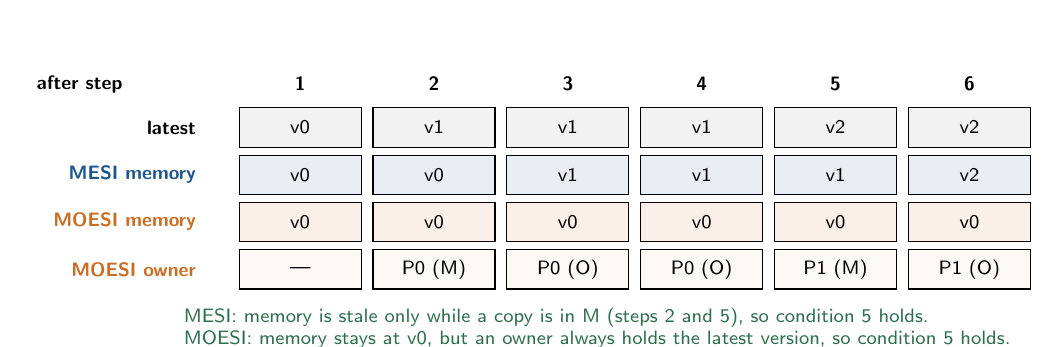
\begin{tikzpicture}[font=\sffamily\scriptsize,
    cell/.style={draw, minimum width=1.55cm, minimum height=0.5cm, align=center},
    hd/.style={font=\sffamily\bfseries\scriptsize}]
  \node[hd] at (-1.1,0.55) {after step};
  \foreach \i in {1,...,6} { \node[hd] at (\i*1.7,0.55) {\i}; }
  \node[hd, anchor=east] at (0.5,0) {latest};
  \node[hd, anchor=east, text=mesiBlue] at (0.5,-0.6) {MESI memory};
  \node[hd, anchor=east, text=moesiOrange] at (0.5,-1.2) {MOESI memory};
  \node[hd, anchor=east, text=moesiOrange] at (0.5,-1.8) {MOESI owner};
  \foreach \i/\l/\m/\o/\w in {1/v0/v0/v0/---, 2/v1/v0/v0/P0 (\stM), 3/v1/v1/v0/P0 (\stO), 4/v1/v1/v0/P0 (\stO), 5/v2/v1/v0/P1 (\stM), 6/v2/v2/v0/P1 (\stO)} {
    \node[cell, fill=coreGrey!8] at (\i*1.7,0) {\l};
    \node[cell, fill=mesiBlue!10] at (\i*1.7,-0.6) {\m};
    \node[cell, fill=moesiOrange!10] at (\i*1.7,-1.2) {\o};
    \node[cell, fill=moesiOrange!5] at (\i*1.7,-1.8) {\w};
  }
  \node[text=memGreen, align=left, anchor=west] at (0.1,-2.55)
    {MESI: memory is stale only while a copy is in \stM\ (steps 2 and 5), so condition 5 holds.\\
     MOESI: memory stays at v0, but an owner always holds the latest version, so condition 5 holds.};
\end{tikzpicture}
\end{bigfig}
\caption[Version-number check]{Versions on the six-step trace. Writes create new
versions at steps 2 and~5. In MESI the forced writebacks at steps 3 and~6 bring
memory up to date; in MOESI memory is never written during the trace, which is
correct only because an owner always has the latest version.}
\label{fig:versions}
\end{figure}

% ===============================================================
%  Chapter 16 -- The Dirty Sharing Ratio
% ===============================================================
\chapter{The Dirty Sharing Ratio: Predicting the Benefit of MOESI}
\label{ch:dsr}
\index{MOESI}\index{Dirty Sharing Ratio}%

\begin{figure}[htbp]
\centering
\adjustbox{max width=\linewidth}{%
\begin{forest}
  chapter map,
  [Chapter 16
    [Definition [One counter under MESI] [Worked example]]
    [Dirty epochs [Write to next write] [Where write backs fall]]
    [Saving identity [MOESI never sends more] [{$S=\sigma\cdot72\,\dsr/\bar b$}]]
    [Patterns {\&} mixtures [Survival fraction]]
    [From bytes to time [Two effects of \stO] [Bus load]]
    [Hypotheses [H1 to H4] [Our contributions]]
  ]
\end{forest}}
\caption[]{Structure of Chapter~16: the metric, its exact
meaning through dirty epochs, the identity linking it to MOESI's saving, the step
from bytes to time, and four testable hypotheses.}
\label{fig:ch16-map}
\end{figure}

% ---------------------------------------------------------------
\section{Definition}
\label{sec:dsr-def}
\sectionmap{[DSR [Coherence transactions under MESI] [Reads served by a modified copy]
  [Two counters] [Worked example]]}
\index{MESI}\index{MOESI}\index{forced writeback}\index{Dirty Sharing Ratio}\index{snooping protocol}%

RQ3 asks whether the benefit of removing forced writebacks can be predicted from a
workload's behaviour under MESI. A predictor that needs a MOESI run is no use, so
we want a quantity a MESI system can count with almost no extra hardware. Every bus
transaction under MESI is a read miss, a write miss or an upgrade, and we call
their total the number of coherence transactions $n_{\mathrm{tx}}$. Some read
misses find the block in another cache in \stM, and each of these causes a forced
writeback. We call their number $n_{\mathrm{dr}}$ (dirty reads).

\begin{keybox}[Definition: Dirty Sharing Ratio]
\[
  \dsr(W,N) \;=\; \frac{n_{\mathrm{dr}}}{n_{\mathrm{tx}}}
  \;=\; \frac{\text{read misses served by a cache holding the block in \stM}}
             {\text{read misses} + \text{write misses} + \text{upgrades}},
\]
measured while workload $W$ runs on $N$ cores under MESI.
\end{keybox}

On a snooping bus, a cache holding the requested block in \stM\ already announces
that it will supply and flush the data (\cref{fig:snoop-bus}). Counting the bus
cycles with that announcement gives $n_{\mathrm{dr}}$, and counting all
transactions gives $n_{\mathrm{tx}}$. Both events are visible to the bus arbiter,
so two counters are enough (\cref{fig:dsr-counter}). Our simulator keeps the two
counts directly. For the six-step trace priced in \cref{tab:mesi-bill}, MESI makes
five coherence transactions (read misses at steps 1, 3, 4 and~6 and the upgrade at
step~5), and two of the read misses (steps 3 and~6) find the block in \stM, so
\begin{equation}
  \dsr = \tfrac{2}{5} = 0.40 .
  \label{eq:dsr-example}
\end{equation}

\begin{figure}[htbp]
\centering
\begin{bigfig}[0.92]
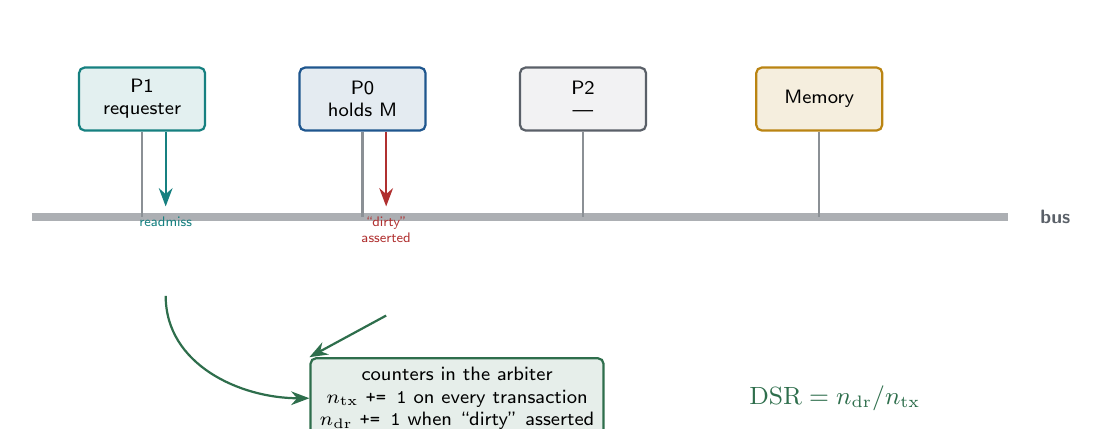
\begin{tikzpicture}[font=\sffamily\scriptsize,
    cc/.style={draw, thick, rounded corners=2pt, minimum width=1.6cm, minimum height=0.8cm, align=center},
    ar/.style={-{Stealth}, thick}]
  \draw[line width=3pt, coreGrey!50] (-0.6,0) -- (11.8,0);
  \node[font=\sffamily\bfseries\scriptsize, text=coreGrey] at (12.4,0) {bus};
  \node[cc, fill=tealC!12, draw=tealC] (r) at (0.8,1.5) {P1\\requester};
  \node[cc, fill=mesiBlue!12, draw=mesiBlue] (h) at (3.6,1.5) {P0\\holds \stM};
  \node[cc, fill=coreGrey!8, draw=coreGrey] (p2) at (6.4,1.5) {P2\\---};
  \node[cc, fill=amberC!14, draw=amberC] (mem) at (9.4,1.5) {Memory};
  \foreach \n in {r,h,p2,mem} { \draw[thick, coreGrey!70] (\n.south) -- (\n.south|-0,0); }
  \draw[ar, tealC] (r.south) ++(0.3,0) -- ++(0,-0.95) node[below, font=\sffamily\tiny]{readmiss};
  \draw[ar, alertRed] (h.south) ++(0.3,0) -- ++(0,-0.95) node[below, font=\sffamily\tiny, align=center]{``dirty''\\asserted};
  \node[cc, fill=memGreen!12, draw=memGreen, minimum width=2.6cm] (cnt) at (4.8,-2.3)
     {counters in the arbiter\\$n_{\mathrm{tx}}$ \texttt{+= 1} on every transaction\\$n_{\mathrm{dr}}$ \texttt{+= 1} when ``dirty'' asserted};
  \draw[ar, memGreen] (3.9,-1.25) -- (cnt.north west);
  \draw[ar, memGreen] (1.1,-1.0) to[out=-90, in=180] (cnt.west);
  \node[text=memGreen, font=\sffamily\bfseries\small] at (9.6,-2.3) {$\dsr = n_{\mathrm{dr}} / n_{\mathrm{tx}}$};
\end{tikzpicture}
\end{bigfig}
\caption[Measuring the Dirty Sharing Ratio]{Measuring DSR on a MESI snooping bus.
The holder of a modified block already signals that it will supply the data, so
two counters give the metric.}
\label{fig:dsr-counter}
\end{figure}

\Cref{tab:dsr-example} carries the example through to MOESI. MOESI saves 72 of
MESI's 472 bytes, or 15.3\,\%, which is half the 30.5\,\% of forced writebacks
counted in Chapter~7. The forced writeback at step~3 disappears, because P0's owned
copy is made obsolete by P1's write at step~5 and never needs to reach memory. The
one at step~6 is only deferred: P1 still owns the block when the run ends and pays
the writeback then.

\begin{table}[htbp]
\centering
\caption{The six-step trace of \cref{tab:trace} under MESI and MOESI, with bytes
from \cref{tab:counting-rules}. ``Drain'' charges one writeback at the end for
each block still dirty.}
\label{tab:dsr-example}
\small
\begin{tabular}{@{}c l c c c c l@{}}
\toprule
Step & Access & Transaction & Dirty read? & MESI B & MOESI B & Epoch \\
\midrule
1 & P0 reads  & read miss & no  & 80  & 80 & --- \\
2 & P0 writes & (silent)  & --- & 0   & 0  & 1 opens (P0) \\
3 & P1 reads  & read miss & \textbf{yes} & 152 & 80 & 1 \\
4 & P2 reads  & read miss & no  & 80  & 80 & 1 \\
5 & P1 writes & upgrade   & --- & 8   & 8  & 1 ends; 2 opens (P1) \\
6 & P0 reads  & read miss & \textbf{yes} & 152 & 80 & 2 \\
end & drain   & ---       & --- & 0   & 72 & 2 ends \\
\midrule
 & \textbf{Total} & 5 & 2 & \textbf{472} & \textbf{400} & \\
\bottomrule
\end{tabular}
\end{table}

% ---------------------------------------------------------------
\section{Dirty Epochs}
\label{sec:dsr-epochs}
\sectionmap{[Epochs [From one write to the next] [At most one write back each]
  [MESI pays if anyone reads] [MOESI pays if the owner leaves]]}
\index{MESI}\index{MOESI}\index{Owned state}\index{forced writeback}\index{dirty epoch}\index{owner}%

Fix one block. A \gls{epoch}\index{dirty epoch} starts when some core writes the
block and ends at the next write to it by any core, or at the end of the run.
During an epoch the value does not change, and one core, the last writer, holds the
newest data when the epoch starts. Epochs divide the whole history of a block, so
each writeback of the block falls in some epoch (\cref{fig:epoch}). Both protocols
write a block back only when a dirty copy stops being dirty, and after the first
writeback in an epoch no dirty copy is left until the next write, so each protocol
makes at most one writeback per epoch. MESI writes back if the epoch has at least
one remote read (the forced writeback, at the first one), or otherwise if the
writer evicts its \stM\ copy before the epoch ends. MOESI writes back if and only if
the owner's copy (\stM\ or \stO) is evicted, or the run ends, before the epoch ends.
The two differ in one case only: an epoch with at least one remote read in which
the owner keeps the block until the next write. MESI pays a writeback there and
MOESI does not, and we call such an epoch \emph{saved}.

\begin{figure}[htbp]
\centering
\begin{bigfig}[0.92]
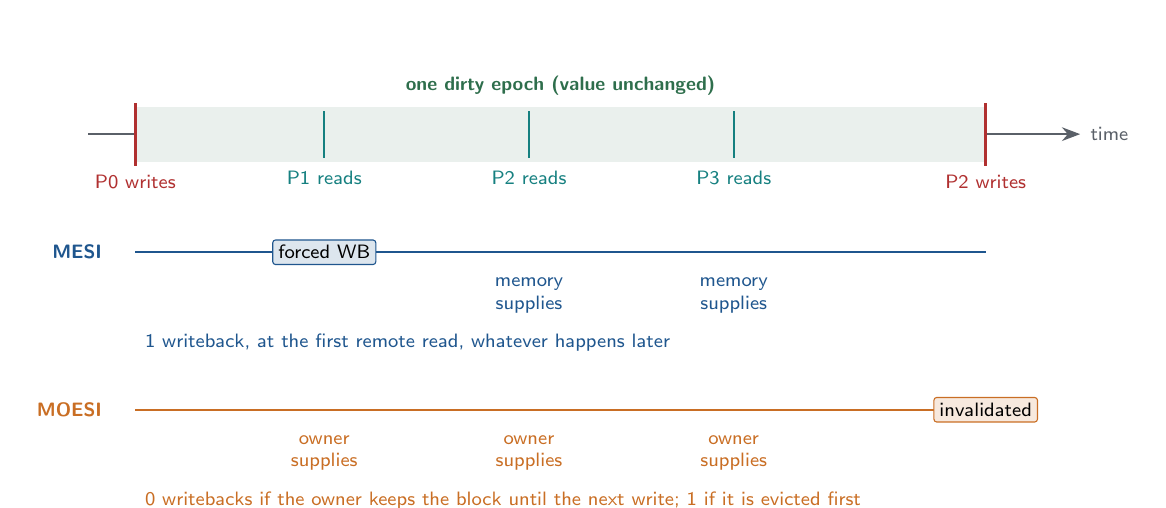
\begin{tikzpicture}[font=\sffamily\scriptsize]
  \draw[-{Stealth}, thick, coreGrey] (0,0) -- (12.6,0) node[right]{time};
  \fill[memGreen!10] (0.6,-0.35) rectangle (11.4,0.35);
  \node[font=\sffamily\bfseries\scriptsize, text=memGreen] at (6.0,0.62) {one dirty epoch (value unchanged)};
  \foreach \x/\t in {0.6/{P0 writes}, 11.4/{P2 writes}} {
     \draw[very thick, alertRed] (\x,-0.4) -- (\x,0.4); \node[text=alertRed, below] at (\x,-0.4) {\t}; }
  \foreach \x/\t in {3.0/{P1 reads}, 5.6/{P2 reads}, 8.2/{P3 reads}} {
     \draw[thick, tealC] (\x,-0.3) -- (\x,0.3); \node[text=tealC, below] at (\x,-0.35) {\t}; }
  \node[anchor=east, text=mesiBlue, font=\sffamily\bfseries\scriptsize] at (0.3,-1.5) {MESI};
  \draw[mesiBlue, thick] (0.6,-1.5) -- (11.4,-1.5);
  \node[draw=mesiBlue, fill=mesiBlue!15, rounded corners=1pt, inner sep=2pt] at (3.0,-1.5) {forced WB};
  \node[text=mesiBlue, align=center] at (5.6,-2.05) {memory\\supplies};
  \node[text=mesiBlue, align=center] at (8.2,-2.05) {memory\\supplies};
  \node[text=mesiBlue, anchor=west] at (0.6,-2.65) {1 writeback, at the first remote read, whatever happens later};
  \node[anchor=east, text=moesiOrange, font=\sffamily\bfseries\scriptsize] at (0.3,-3.5) {MOESI};
  \draw[moesiOrange, thick] (0.6,-3.5) -- (11.4,-3.5);
  \foreach \x in {3.0,5.6,8.2} { \node[text=moesiOrange, align=center] at (\x,-4.05) {owner\\supplies}; }
  \node[draw=moesiOrange, fill=moesiOrange!15, rounded corners=1pt, inner sep=2pt] at (11.4,-3.5) {invalidated};
  \node[text=moesiOrange, anchor=west] at (0.6,-4.65) {0 writebacks if the owner keeps the block until the next write; 1 if it is evicted first};
\end{tikzpicture}
\end{bigfig}
\caption[A dirty epoch]{One dirty epoch with three remote reads. MESI pays one
writeback at the first remote read and memory serves later readers. MOESI pays
nothing while the owner keeps the block, and the value becomes obsolete at the next
write.}
\label{fig:epoch}
\end{figure}

% ---------------------------------------------------------------
\section{The Saving Identity}
\label{sec:dsr-identity}
\sectionmap{[Identity [MOESI never sends more bytes] [Saving = 72 per saved epoch]
  [Survival fraction sigma] [{$S=\sigma\cdot72\,\dsr/\bar b$}]]}
\index{MESI}\index{MOESI}\index{Dirty Sharing Ratio}\index{survival fraction}\index{dirty epoch}\index{sharing patterns!producer--consumer}\index{sharing patterns!migratory}\index{owner}\index{proof}%

\begin{proposition}[MOESI never sends more bytes]
\label{prop:never-worse}
Under the method of Chapter~15 and the counting rules of
\cref{tab:counting-rules}, for every trace $W$,
\[
  0 \;\le\; \Delta B(W) \;=\; 72\, n_{\mathrm{saved}}(W) \;\le\; 72\, n_{\mathrm{dr}}(W),
\]
where $n_{\mathrm{saved}}$ is the number of saved epochs and $n_{\mathrm{dr}}$ the
number of dirty reads under MESI.
\end{proposition}

\noindent The proof is in \cref{app:proof-never-worse}. It compares the two
protocols epoch by epoch using \cref{prop:residency}, and notes that each saved
epoch contains exactly one dirty read. Two consequences follow. In the traffic
model MOESI cannot lose, so any loss has to come from timing (\cref{sec:dsr-time}).
And the dirty reads that DSR counts are exactly the epochs MOESI could save. The
fraction it does save is the \gls{sigma}
\begin{equation}
  \sigma = \frac{n_{\mathrm{saved}}}{n_{\mathrm{dr}}} \in [0,1],
  \label{eq:sigma}
\end{equation}
the share of dirty-read epochs whose owner keeps the block until the next write.
Large caches and frequent rewriting push $\sigma$ towards~1, while small caches,
which evict owners early, and runs that end with many blocks still owned push it
down. Dividing $\Delta B$ by MESI's total bytes, writing $\bar b =
B_{\mathrm{MESI}}/n_{\mathrm{tx}}$ for the average bytes MESI moves per coherence
transaction (writebacks included), and using $n_{\mathrm{dr}} = \dsr\cdot
n_{\mathrm{tx}}$ gives the central result of this chapter.

\begin{keybox}[The saving identity]
\begin{equation}
  S_B \;=\; \frac{\Delta B}{B_{\mathrm{MESI}}}
      \;=\; \sigma\,\frac{72\; n_{\mathrm{dr}}}{B_{\mathrm{MESI}}}
      \;=\; \sigma \cdot F \;=\; \sigma\cdot\frac{72\,\dsr}{\bar b}.
  \label{eq:identity}
\end{equation}
The share of traffic MOESI saves equals the survival fraction times the
forced-writeback fraction of \cref{eq:fwb-fraction}. Equivalently, it is
proportional to DSR with constant $72\sigma/\bar b$.
\end{keybox}

The identity agrees with the earlier examples. For the six-step trace, $\dsr=0.4$,
$\bar b = 472/5 = 94.4$\,B and $\sigma = 1/2$ (one of the two dirty-read epochs is
saved), so $0.5\times72\times0.4/94.4 = 15.3\,\%$, as in \cref{tab:dsr-example}.
For the migratory trace of \cref{tab:method-example} the block has four epochs,
opened at steps 2, 4, 6 and~8. The first three each have one remote read and end at
the next write with the owner still holding the block, so all three are saved; the
fourth has no remote read. Then $n_{\mathrm{dr}}=3$, $n_{\mathrm{tx}}=7$, $\sigma=1$
and $\bar b = 632/7 \approx 90.3$\,B, giving $72\times(3/7)/90.3 = 216/632 =
34.2\,\%$. For the producer--consumer model of \cref{eq:pc-model} with $C$
consumers, each round has $C+1$ transactions of which one is a dirty read, so
$\dsr = 1/(C+1)$ and $\bar b = (160+80(C-1))/(C+1)$. In steady state the producer
always keeps the block, so $\sigma=1$ and \cref{eq:identity} becomes
$72/(160+80(C-1))$, which is 45\,\% for $C=1$, as in \cref{tab:traffic-patterns}.

\Cref{eq:identity} is exact, but besides DSR it contains $\bar b$, which is easy to
measure under MESI, and $\sigma$, which depends on what happens after each dirty
read. The predictor we propose is therefore
\begin{equation}
  \hat S_B = \frac{72\,\dsr}{\bar b}\qquad(\sigma\text{ taken as }1),
  \label{eq:predictor}
\end{equation}
which overestimates the saving by the factor $1/\sigma$. When $\bar b$ varies little
between workloads, $\hat S_B$ is close to a straight line in DSR with slope
$72/\bar b$ (\cref{fig:identity-lines}). How close $\sigma$ stays to~1 and how much
$\bar b$ varies cannot be derived in general; Part~VI measures both.

\begin{figure}[htbp]
\centering
\adjustbox{max width=\linewidth}{%
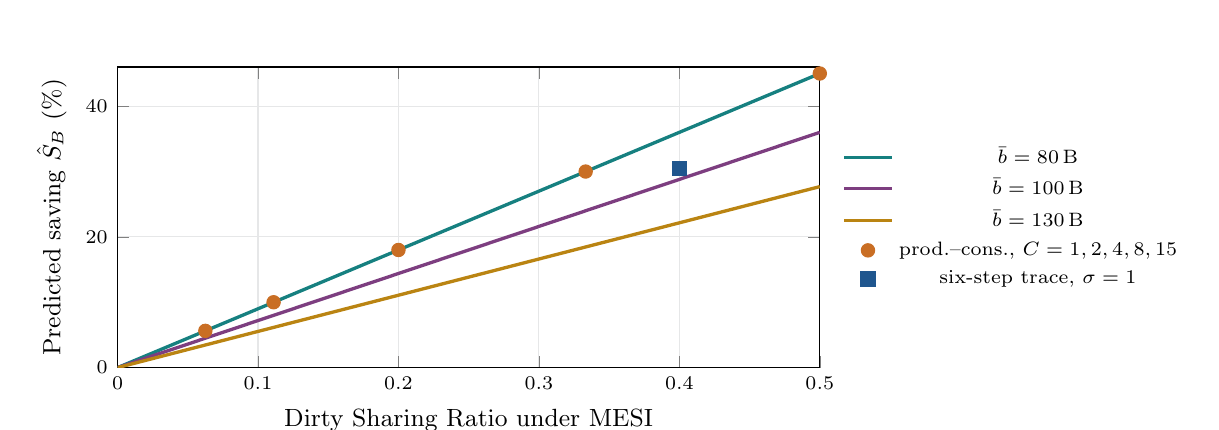
\begin{tikzpicture}
  \begin{axis}[width=10.5cm, height=5.4cm,
      xlabel={Dirty Sharing Ratio under MESI}, ylabel={Predicted saving $\hat S_B$ (\%)},
      xmin=0, xmax=0.5, ymin=0, ymax=46, xtick={0,0.1,0.2,0.3,0.4,0.5},
      xticklabel style={/pgf/number format/fixed, /pgf/number format/precision=1},
      legend style={at={(1.02,0.5)}, anchor=west, font=\scriptsize, draw=none},
      grid=major, grid style={coreGrey!15},
      label style={font=\small}, tick label style={font=\scriptsize}]
    \addplot[very thick, tealC, domain=0:0.5] {7200*x/80};   \addlegendentry{$\bar b = 80$\,B}
    \addplot[very thick, plumC, domain=0:0.5] {7200*x/100};  \addlegendentry{$\bar b = 100$\,B}
    \addplot[very thick, amberC, domain=0:0.5] {7200*x/130}; \addlegendentry{$\bar b = 130$\,B}
    \addplot[only marks, mark=*, mark size=2.4pt, moesiOrange] coordinates
      {(0.5,45) (0.3333,30) (0.2,18) (0.1111,10) (0.0625,5.625)};
    \addlegendentry{prod.--cons., $C=1,2,4,8,15$}
    \addplot[only marks, mark=square*, mark size=2.6pt, mesiBlue] coordinates {(0.4,30.5)};
    \addlegendentry{six-step trace, $\sigma=1$}
  \end{axis}
\end{tikzpicture}}
\caption[The predictor as a family of lines]{\Cref{eq:predictor} for three values of
$\bar b$. The producer--consumer model lies on the 80\,B line because each round
moves $80(C+1)$ bytes in $C+1$ transactions. The blue square is the six-step trace
($\bar b=94.4$\,B) if its last epoch were also saved. Analytical.}
\label{fig:identity-lines}
\end{figure}

% ---------------------------------------------------------------
\section{The Sharing Patterns and Their Mixtures}
\label{sec:dsr-patterns}
\sectionmap{[Patterns [DSR of each pattern] [Mixtures weighted by transactions]
  [A little dirty sharing goes a long way] [Survival fraction]]}
\index{MESI}\index{MOESI}\index{dirty sharing}\index{Dirty Sharing Ratio}\index{survival fraction}\index{dirty epoch}\index{sharing patterns!producer--consumer}\index{sharing patterns!migratory}\index{LRU replacement}\index{owner}%

\Cref{tab:dsr-patterns} applies the definition to one unit of each sharing pattern
of \cref{tab:patterns}, in steady state and with caches large enough that owners
are not evicted; the entries follow from the transaction counts of
\cref{tab:traffic-patterns}. Private and read-only data never involve dirty data
read by another core, so their DSR is zero and MOESI saves nothing on them. The two
dirty-sharing patterns both have $\bar b = 80$\,B, which is why their savings lie on
one line of \cref{fig:identity-lines}. Migratory sharing has the largest DSR in the
table, one half, since every hand-off is one dirty read and one upgrade.

\begin{table}[htbp]
\centering
\caption{The Dirty Sharing Ratio and the saving identity for one unit of each
sharing pattern ($C$ consumers per producer write), in steady state with no
capacity evictions. $S_B$ from \cref{eq:identity}.}
\label{tab:dsr-patterns}
\small
\begin{tabular}{@{}L{3.1cm} c c c c c c@{}}
\toprule
Pattern (unit) & $n_{\mathrm{tx}}$ & $n_{\mathrm{dr}}$ & $\dsr$ & $\bar b$ (B) &
  $\sigma$ & $S_B$ \\
\midrule
Private (read, write, evict) & 1 & 0 & 0 & 152 & --- & 0 \\
Read-only (per reader) & 1 & 0 & 0 & 80 & --- & 0 \\
Producer--consumer (per round) & $C+1$ & 1 & $\frac{1}{C+1}$ & 80 & 1 &
  $\frac{0.9}{C+1}$ \\
Migratory (per hand-off) & 2 & 1 & $\frac{1}{2}$ & 80 & 1 & 45\,\% \\
\bottomrule
\end{tabular}
\end{table}

A real program mixes the patterns. DSR is a ratio of transaction counts, so the DSR
of a mixture is the average of the patterns' DSRs weighted by the transactions each
produces, not by its accesses:
\begin{equation}
  \dsr_{\mathrm{mix}} = \frac{\sum_i n_{\mathrm{dr},i}}{\sum_i n_{\mathrm{tx},i}}
  = \frac{\sum_i n_{\mathrm{tx},i}\,\dsr_i}{\sum_i n_{\mathrm{tx},i}} .
  \label{eq:dsr-mix}
\end{equation}
Private data that mostly hits produces few transactions, so a small amount of
migratory or producer--consumer sharing can dominate the DSR. If a fraction $m$ of
all accesses go to migratory blocks (one transaction each, $\dsr = 1/2$) and the
rest are private accesses with hit rate $h$ ($1-h$ transactions each, $\dsr=0$),
\begin{equation}
  \dsr_{\mathrm{mix}}(m,h) = \frac{m/2}{m + (1-m)(1-h)} .
  \label{eq:dsr-mix-mig}
\end{equation}
With a 99\,\% private hit rate, 1\,\% of migratory accesses already gives a DSR of
0.25, half the maximum (\cref{fig:dsr-mix}). A workload's DSR can therefore be high
even when sharing is a small part of its accesses, and the identity ties MOESI's
saving to the DSR, not to the share of accesses.

\begin{figure}[htbp]
\centering
\begin{minipage}[c]{0.54\linewidth}\centering
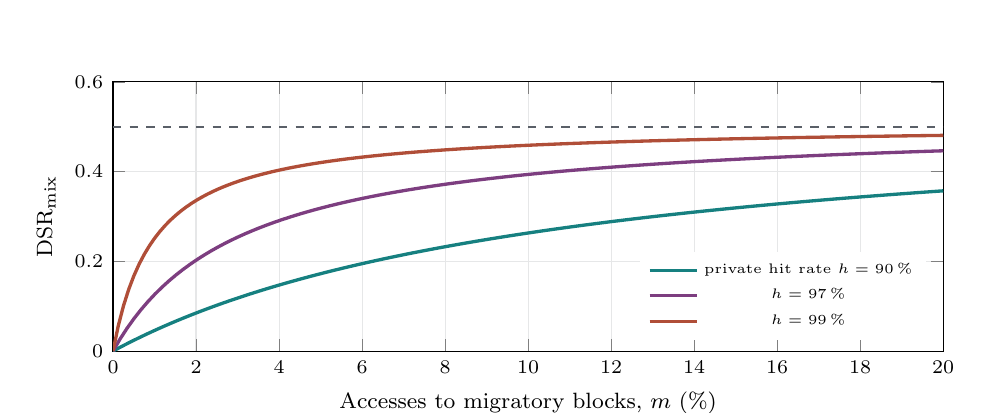
\begin{tikzpicture}
  \begin{axis}[width=\linewidth, height=5.0cm,
      xlabel={Accesses to migratory blocks, $m$ (\%)}, ylabel={$\dsr_{\mathrm{mix}}$},
      xmin=0, xmax=20, ymin=0, ymax=0.6,
      legend style={at={(0.98,0.04)}, anchor=south east, font=\tiny, draw=none, fill=white},
      grid=major, grid style={coreGrey!15},
      label style={font=\footnotesize}, tick label style={font=\scriptsize}]
    \addplot[very thick, tealC, domain=0:20, samples=120] {(x/100/2)/((x/100) + (1-x/100)*0.10)};
      \addlegendentry{private hit rate $h = 90\,\%$}
    \addplot[very thick, plumC, domain=0:20, samples=120] {(x/100/2)/((x/100) + (1-x/100)*0.03)};
      \addlegendentry{$h = 97\,\%$}
    \addplot[very thick, brickC, domain=0:20, samples=160] {(x/100/2)/((x/100) + (1-x/100)*0.01)};
      \addlegendentry{$h = 99\,\%$}
    \addplot[thick, dashed, coreGrey, forget plot] coordinates {(0,0.5) (20,0.5)};
  \end{axis}
\end{tikzpicture}
\caption[DSR of a mixture]{\Cref{eq:dsr-mix-mig}: a few per cent of migratory
accesses dominate the metric (dashed: the migratory maximum, 0.5). Analytical.}
\label{fig:dsr-mix}
\end{minipage}\hfill
\begin{minipage}[c]{0.43\linewidth}\centering
\adjustbox{max width=\linewidth}{%
\begin{forest}
  decision tree,
  [{One dirty epoch}
    [{Any remote read\\before the next write?}
      [{Owner evicted\\before next write?}, el=yes
        [{Deferred\\(lowers $\sigma$)}, el=yes]
        [{Run ends\\first?}, el=no
          [{Deferred:\\paid at end}, el=yes]
          [{Saved}, el=no]]]
      [{Nothing\\to save}, el=no]]
  ]
\end{forest}}
\caption[Is an epoch saved?]{Classifying a dirty epoch. The fraction of dirty-read
epochs that are saved is $\sigma$.}
\label{fig:sigma-tree}
\end{minipage}
\end{figure}

The remaining unknown is $\sigma$. \Cref{fig:sigma-tree} gives the test for one
epoch. Under the method of Chapter~15 the owner's copy is evicted at the same moment
in both protocols (\cref{prop:residency}), so $\sigma$ is a property of the workload
and the cache, not of the protocol. Two things lower it. The first is capacity: if
the owner touches more distinct blocks during the epoch than its cache can hold, LRU
evicts the owned block before the next write, and the writeback MESI paid early is
paid late instead. Small caches, large working sets and long epochs all make this
more likely. The second is the end of the run: epochs still open when measurement
stops are charged a writeback, as at step~6 of \cref{tab:dsr-example}. Over a long
run this is a small fixed number of epochs, so its effect shrinks, but in a short
trace such as the six-step one it can halve the saving.

% ---------------------------------------------------------------
\section{From Bytes to Time}
\label{sec:dsr-time}
\sectionmap{[Time [O changes two things] [Write back removed]
  [Owner answers later reads] [Latency per epoch] [Load decides]]}
\index{MESI}\index{MOESI}\index{Owned state}\index{forced writeback}\index{dirty epoch}\index{AMAT}\index{bus utilisation}\index{cache-to-cache transfer}\index{Effect A and Effect B}\index{coherence miss}%

RQ2 asks whether saved bytes become saved time, and RQ4 whether deferring
writebacks can cost more than it saves. With the controlled method we can see that
\stO\ changes two things, with different signs (\cref{fig:two-effects}).

\begin{figure}[htbp]
\centering
\adjustbox{max width=0.95\linewidth}{%
\begin{forest}
  chapter map,
  [What \stO\ changes
    [{Effect A: write back removed}
      [{at the first remote read of an epoch}]
      [{saves bus and memory occupancy}]
      [{and the reader's wait for the flush}]
      [{sign: always helps}]]
    [{Effect B: owner answers later reads}
      [{readers 2, 3, ... of the epoch}]
      [{cache-to-cache instead of memory}]
      [{faster if $T_{\mathrm{c2c}} < T_{\mathrm{mem}}$}]
      [{sign: helps or hurts}]]
  ]
\end{forest}}
\caption[Two effects of the Owned state]{The \stO\ state bundles two effects.
Effect~A, removing the forced writeback, is the subject of this report; Effect~B
changes the supplier for later readers. Only Effect~A always helps.}
\label{fig:two-effects}
\end{figure}

Take a saved epoch with $r\ge1$ remote reads on an otherwise idle bus. Let
$T_{\mathrm{coh}}$ be the time for a read served by a cache holding the block in
\stM\ under MESI, including the writeback (as in \cref{eq:amat-coh}); let
$t_{\mathrm{wb}}$ be the part spent transferring the writeback; let
$T_{\mathrm{c2c}} = T_{\mathrm{coh}} - t_{\mathrm{wb}}$ be a cache-to-cache read
without a writeback; and let $T_{\mathrm{mem}}$ be a read served by memory. Under
MESI the first reader waits $T_{\mathrm{coh}}$ and the other $r-1$ wait
$T_{\mathrm{mem}}$, while under MOESI all $r$ wait $T_{\mathrm{c2c}}$. The reader
latency saved in the epoch is
\begin{equation}
  \Delta L(r) \;=\; \underbrace{\bigl(T_{\mathrm{coh}} - T_{\mathrm{c2c}}\bigr)}_{\text{Effect A}\;=\;t_{\mathrm{wb}}}
  \;+\; \underbrace{(r-1)\bigl(T_{\mathrm{mem}} - T_{\mathrm{c2c}}\bigr)}_{\text{Effect B}} .
  \label{eq:dL}
\end{equation}
With the assumed $T_{\mathrm{coh}}=60$ and $T_{\mathrm{mem}}=100$ cycles (Chapters~2
and~8) and the 9-cycle transfer of a 72-byte writeback on the 8-byte-per-cycle bus
of Chapter~17, Effect~A is 9 cycles per saved epoch and Effect~B is $100-51 = 49$
cycles per extra reader. Effect~B changes sign once a cache-to-cache read is slower
than a memory read (\cref{fig:dL}). With $T_{\mathrm{c2c}}=141$ cycles, for
example, an epoch with three readers loses $9-2\times41 = -73$ cycles under MOESI.

\begin{figure}[htbp]
\centering
\adjustbox{max width=\linewidth}{%
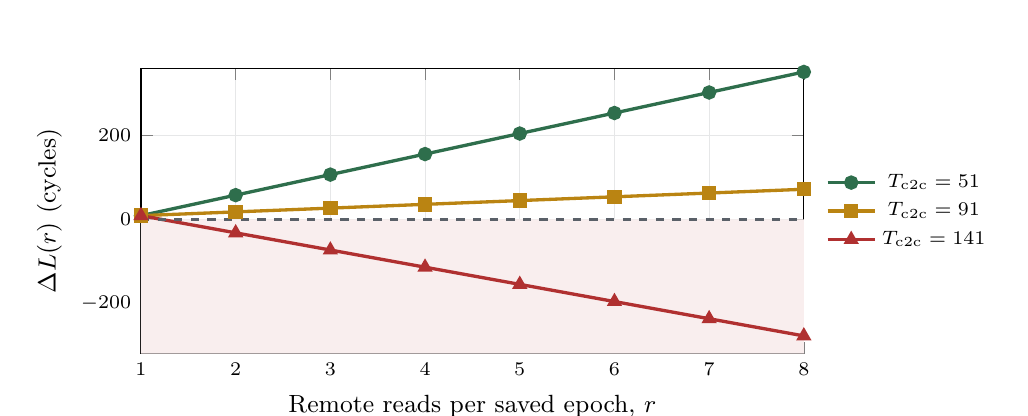
\begin{tikzpicture}
  \begin{axis}[width=10cm, height=5.2cm,
      xlabel={Remote reads per saved epoch, $r$}, ylabel={$\Delta L(r)$ (cycles)},
      xmin=1, xmax=8, ymin=-320, ymax=360, xtick={1,...,8},
      legend style={at={(1.02,0.5)}, anchor=west, font=\scriptsize, draw=none},
      grid=major, grid style={coreGrey!15},
      label style={font=\small}, tick label style={font=\scriptsize}]
    \addplot[fill=alertRed!8, draw=none, forget plot] coordinates {(1,0) (8,0) (8,-320) (1,-320)} \closedcycle;
    \addplot[very thick, memGreen, mark=*, domain=1:8, samples=8] {9 + (x-1)*(100-51)};
      \addlegendentry{$T_{\mathrm{c2c}} = 51$}
    \addplot[very thick, amberC, mark=square*, domain=1:8, samples=8] {9 + (x-1)*(100-91)};
      \addlegendentry{$T_{\mathrm{c2c}} = 91$}
    \addplot[very thick, alertRed, mark=triangle*, domain=1:8, samples=8] {9 + (x-1)*(100-141)};
      \addlegendentry{$T_{\mathrm{c2c}} = 141$}
    \addplot[thick, dashed, coreGrey, forget plot] coordinates {(1,0) (8,0)};
  \end{axis}
\end{tikzpicture}}
\caption[Latency saved per epoch]{\Cref{eq:dL} with $T_{\mathrm{mem}}=100$ and
$t_{\mathrm{wb}}=9$ cycles. Effect~A gives each saved epoch 9 cycles; Effect~B adds
or subtracts $T_{\mathrm{mem}}-T_{\mathrm{c2c}}$ per further reader (shaded: MOESI
slower). Analytical, idle bus.}
\label{fig:dL}
\end{figure}

\Cref{eq:dL} ignores waiting. On a bus that carries one message at a time
(\cref{eq:util}) every transaction also occupies the bus, and under MESI a dirty
read occupies it for one more 72-byte message. On a lightly used bus requests rarely
wait, so the occupancy MOESI saves shortens almost nothing, and execution time
changes only by the latency of \cref{eq:dL}, spread over a run dominated by
computation and hits. As utilisation nears 100\,\% waiting grows sharply
(Chapter~8), execution time is set by the total time the bus is busy, and the
speed-up of MOESI tends to the ratio of bus-busy times,
\begin{equation}
  \frac{T(\mathrm{MESI})}{T(\mathrm{MOESI})} \;\longrightarrow\;
  \frac{C_{\mathrm{bus}}(\mathrm{MESI})}{C_{\mathrm{bus}}(\mathrm{MOESI})}
  \qquad\text{as } U \to 100\,\%,
  \label{eq:sat-limit}
\end{equation}
where $C_{\mathrm{bus}}$ is the total number of cycles the bus is occupied. By
\cref{prop:residency} the two runs differ in $C_{\mathrm{bus}}$ only by the
occupancy of the writebacks MOESI avoids. The same holds for the memory port, since
every forced writeback is also a 64-byte memory write.

\Cref{eq:amat-coh} shows the low-load case in numbers. Chapter~8 used the 3-cycle
single-core AMAT, $T_{\mathrm{coh}}=60$ cycles and a coherence-miss rate of 1, 2, 4
and 8\,\% at 2, 4, 8 and 16 cores (\cref{fig:amat-bars}). In the case most
favourable to Effect~A, every coherence miss is a dirty read with one reader
($r=1$), so under MOESI each costs $T_{\mathrm{c2c}}=51$ cycles instead of 60
(\cref{tab:amat-compare}). Even then, at 16 cores Effect~A saves 0.72 of 7.8 cycles,
under 10\,\%. A larger time gain has to come from Effect~B or from bus load
(\cref{eq:sat-limit}), which is why H2 below ties the gain to utilisation.

\begin{table}[htbp]
\centering
\caption{AMAT from \cref{eq:amat-coh} with the illustrative values of Chapter~8,
when every coherence miss is a dirty read with one reader. Idle interconnect;
cycles.}
\label{tab:amat-compare}
\small
\begin{tabular}{@{}c c c c c c@{}}
\toprule
Cores & $m_{\mathrm{coh}}$ & AMAT, MESI & AMAT, MOESI & Saved (cycles) & Saved (\%) \\
\midrule
2  & 1\,\% & 3.60 & 3.51 & 0.09 & 2.5 \\
4  & 2\,\% & 4.20 & 4.02 & 0.18 & 4.3 \\
8  & 4\,\% & 5.40 & 5.04 & 0.36 & 6.7 \\
16 & 8\,\% & 7.80 & 7.08 & 0.72 & 9.2 \\
\bottomrule
\end{tabular}
\end{table}

% ---------------------------------------------------------------
\section{Hypotheses and Contributions}
\label{sec:dsr-hypotheses}
\label{sec:contrib-summary}
\sectionmap{[Hypotheses [H1: F falls with cores] [H2: load gates the time gain]
  [H3: DSR predicts the saving] [H4: MOESI loses only through timing] [Contributions C1--C16]]}
\index{MOESI}\index{Dirty Sharing Ratio}\index{survival fraction}\index{directory protocol}\index{sharing patterns!migratory}\index{cache-to-cache transfer}%

The analysis turns each research question of \cref{tab:rq} into a hypothesis that
Part~VI tests (\cref{tab:hypotheses}). We state them here, before any measurement,
so that Part~VI can report where they fail.

\begin{table}[htbp]
\centering
\caption{Hypotheses derived in Part~IV, one per research question, and how each is
tested in Part~VI.}
\label{tab:hypotheses}
\small
\begin{tabular}{@{}l L{5.6cm} L{2.6cm} L{3.4cm}@{}}
\toprule
 & Hypothesis & Basis & Test in Part VI \\
\midrule
H1 (RQ1) & For a fixed sharing structure, $F(W,N)$ falls as $N$ grows,
  because more readers share each epoch: one forced writeback, more 80-byte
  read misses. & \cref{eq:pc-model}, \cref{sec:dsr-epochs} & $F$ measured for
  $N = 2$ to 16 \\
H2 (RQ2) & The execution-time gain of MOESI is near zero at low bus
  utilisation and rises towards the bus-occupancy ratio as utilisation
  approaches 100\,\%. & \cref{eq:dL,eq:sat-limit} & load sweep: gain against
  utilisation \\
H3 (RQ3) & The traffic saving obeys \cref{eq:identity} exactly; with
  $\sigma$ near 1 and $\bar b$ nearly constant, DSR predicts it through
  \cref{eq:predictor}. & \cref{prop:never-worse}, \cref{eq:identity} & DSR
  against measured $S_B$; error of $\hat S_B$ \\
H4 (RQ4) & MOESI never moves more bytes than MESI; it can take more time
  only through Effect~B (when $T_{\mathrm{c2c}} > T_{\mathrm{mem}}$) or owner
  contention. Small caches reduce the gain by lowering $\sigma$ but cannot
  reverse it in bytes. & \cref{prop:never-worse}, \cref{eq:dL} & cache-size
  sweep; latency sensitivity sweep \\
\bottomrule
\end{tabular}
\end{table}

DSR is not the first measure of sharing. Archibald and Baer parameterised their
simulations by the fraction of references to shared
blocks~\cite[p.~286]{archibald1986evaluation}, and adaptive protocols detect
migratory blocks at run time, for example by noticing a write by a processor other
than the last writer~\cite{stenstrom1993adaptive,nilsson1994adaptive}.
\Cref{tab:dsr-vs} shows how DSR differs from these and from $F$. The identity
\cref{eq:identity} is exact only under the method of Chapter~15: one MOESI member,
the same cache contents in both runs, and the counting rules of
\cref{tab:counting-rules}. A directory protocol, another MOESI member or a
non-inclusive hierarchy would change $\bar b$ and could change $\sigma$. DSR also
predicts traffic only; for time, bus load and the relative speed of cache-to-cache
and memory transfers matter as well (\cref{sec:dsr-time}). Part~VII returns to
these limits.

\begin{table}[htbp]
\centering
\caption{The Dirty Sharing Ratio compared with related measures.}
\label{tab:dsr-vs}
\small
\begin{tabular}{@{}L{3.1cm} L{3.0cm} L{3.4cm} L{3.4cm}@{}}
\toprule
Measure & What it counts & Used for & Limitation for RQ3 \\
\midrule
Shared-reference fraction~\cite{archibald1986evaluation} & references to
  shared blocks & input parameter of a model & ignores whether shared data is
  dirty when read \\
Migratory detection~\cite{stenstrom1993adaptive,nilsson1994adaptive} & blocks
  written by successive processors & run-time protocol adaptation & per block,
  inside one protocol; not a workload score \\
Forced-writeback fraction $F$ (\cref{eq:fwb-fraction}) & bytes of forced
  writebacks & definition of the problem & needs byte accounting of all
  messages \\
Dirty Sharing Ratio & dirty reads per transaction & choosing between
  protocols before building one & needs $\bar b$; assumes $\sigma \approx 1$ \\
\bottomrule
\end{tabular}
\end{table}

\label{sec:contrib-parts123}
\label{sec:contrib-parts45}
\Cref{tab:contrib-list} collects what this report adds to the sources it reviews.
C1 to C10 are analytical results reached while studying existing work in Parts~I
to~III; the material they are built from belongs to the cited sources, and the
results are ours. C11 to C16 are the method, metric and tool of Parts~IV and~V. All
analytical results rest on the message sizes of \cref{tab:msg-classes} and the
counting rules of \cref{tab:counting-rules}, including our assumed 16-byte word
update, and C3 to C10 ignore contention, latency and capacity, so they say nothing
about execution time on their own.

\begin{table}[htbp]
\centering
\caption{Contributions of this report. ``Basis'' names the published material
each result is built from.}
\label{tab:contrib-list}
\label{tab:contrib-45}
\footnotesize
\renewcommand{\arraystretch}{1.12}
\begin{tabular}{@{}l L{4.1cm} L{4.6cm} L{3.4cm}@{}}
\toprule
 & Result & What it shows & Where; basis \\
\midrule
C1 & Full MESI state diagrams & completes the textbook's ``exercise for the
  reader'' & \cref{fig:mesi}; \cite[p.~603]{sarangi2025basic} \\
C2 & One trace under MSI, MESI and MOESI & the protocols differ at three points:
  \stE, silent upgrade, \stO & \cref{tab:trace}; \cite{papamarcos1984illinois,sweazey1986moesi} \\
C3 & The trace priced under MESI & writebacks are 30.5\,\% of 472 bytes &
  \cref{tab:mesi-bill} \\
C4 & Producer--consumer model & forced writeback is 72\,B per round: 45\,\% of
  traffic with one consumer, 10\,\% with eight & \cref{eq:pc-model,fig:pc-model} \\
C5 & Superseded-writeback count & over $k$ rounds MESI writes back $k$ times,
  MOESI once & \cref{fig:wasted-timeline,eq:wb-timing} \\
C6 & One counting rule, six protocols, four patterns & ownership saves 45\,\% of
  bytes and every memory write in dirty sharing & \cref{tab:traffic-patterns,fig:bars-pc,fig:bars-mig} \\
C7 & Update versus invalidate crossover & update beats MESI below $w=10$ and
  MOESI below $w=5.5$ & \cref{fig:update-vs-invalidate}; \cite{archibald1986evaluation,thacker1987firefly} \\
C8 & Dirty remote read on point-to-point systems & DASH moves 160\,B and writes
  memory; an owner directory moves 96\,B & \cref{fig:dir-dirty-read,tab:p2p}; \cite{lenoski1990dash} \\
C9 & Five behaviours on one transaction & only the owner outcome shares dirty data
  without a memory write & \cref{fig:remote-read-tree} \\
C10 & Organisation is separate from semantics & a directory changes routing, not
  the writeback & \cref{fig:classes,tab:organisations} \\
\midrule
C11 & Controlled comparison method & MOESI as MESI plus three rules; paired runs &
  \cref{sec:method-delta,sec:method-fixed} \\
C12 & Identical cache contents & the runs differ only in writebacks &
  \cref{prop:residency}, \cref{eq:dB-writebacks} \\
C13 & Dirty Sharing Ratio & measurable with two counters under MESI & \cref{sec:dsr-def} \\
C14 & Dirty epochs and the saving identity & MOESI never moves more bytes;
  $S_B = \sigma\cdot72\,\dsr/\bar b$ & \cref{prop:never-worse}, \cref{eq:identity} \\
C15 & Effect~A and Effect~B & the latency of each, and when B hurts &
  \cref{eq:dL}, \cref{fig:two-effects} \\
C16 & Two-layer simulator & coherence checked on every access; verified against
  every analytical number & Chapter~17 \\
\bottomrule
\end{tabular}
\end{table}

% ===============================================================
%  PART V -- Simulation (Chapters 17--18)
%  The simulator, its verification, the workloads and the experiment
%  configurations. Measurements are in Part VI; code excerpts are in
%  Appendix E (rule 7).
% ===============================================================

\part{Simulation}
\label{part:simulation}

\begin{center}
\adjustbox{max width=\linewidth}{%
\begin{forest}
  part map,
  [Part V
    [Ch.~17: Simulator Design
      [Why our own simulator] [Traffic layer] [Timing layer] [Verification]]
    [Ch.~18: Workloads {\&} Configurations
      [Pattern kernels] [Synthetic mixtures] [Experiments] [Metrics]]
  ]
\end{forest}}
\end{center}

\begin{keybox}[What Part V does]
Chapter~17 describes the two-layer simulator we wrote in Python to apply the
method of Chapter~15. The traffic layer counts every message and byte under MSI,
MESI and MOESI. The timing layer adds per-core clocks, a shared bus and a memory
port, using the latencies assumed earlier in the report. The chapter ends by
checking the simulator against every analytical number of Parts~II to~IV.
Chapter~18 describes the workloads, the experiments and the metrics reported in
Part~VI. Chapter~10 planned to use the \texttt{gem5} full-system
simulator~\cite{binkert2011gem5} and OpenMP programs; \cref{sec:sim-why} explains
why we built the timing model ourselves and used synthetic workloads instead, and
\cref{sec:wl-scope} and Part~VII state what that costs.
\end{keybox}

% ===============================================================
%  Chapter 17 -- Simulator Design
% ===============================================================
\chapter{Simulator Design: A Two-Layer Coherence Simulator}
\label{ch:simulator}

\begin{figure}[htbp]
\centering
\adjustbox{max width=\linewidth}{%
\begin{forest}
  chapter map,
  [Chapter 17
    [Why our own simulator [Control] [Understanding] [Speed]]
    [Traffic layer [Caches {\&} holders] [Protocol rules] [Byte accounting]]
    [Timing layer [Report latencies] [Bus {\&} memory port] [Event loop]]
    [Verification [Analytical numbers] [Coherence checks] [Part IV identities] [Timing checks]]
  ]
\end{forest}}
\caption[]{Structure of Chapter~17: why we built a new
simulator, how its two layers work, and how it was checked before any result was
taken from it.}
\label{fig:ch17-map}
\end{figure}

% ---------------------------------------------------------------
\section{Why Build Our Own Simulator}
\label{sec:sim-why}
\label{sec:sim-arch}
\sectionmap{[Choice [Method needs one changed variable] [Team must understand every line]
  [Fast enough to sweep] [What we give up]]}
\index{MESI}\index{MOESI}\index{gem5}\index{simulator!traffic layer}\index{simulator!timing layer}%

Coherence studies usually use an established simulator such as
\texttt{gem5}~\cite{binkert2011gem5}, which models pipelines, caches, interconnects
and DRAM cycle by cycle, runs real programs and comes with several coherence
protocols. Three needs of this report pointed the other way. The method of
Chapter~15 requires MESI and MOESI to differ only in the three rules of
\cref{tab:transition-diff}, while the protocols shipped with a large simulator are
separate implementations that differ in many more ways, the situation of
\cref{fig:method-idea}(a); rewriting one to match the other would have been a
project of its own. Every result in Part~VI also had to be something we could
explain from first principles, which a few hundred lines whose rules are the tables
of this report allow and a large external code base does not. And testing H1 to H4
needs hundreds of paired runs, which our simulator finishes in about a minute on a
two-core machine (\cref{tab:sim-choice}). The price is realism: no pipeline, no
DRAM model and no real programs. We therefore report trends and approximate sizes,
not predictions of any real machine's run time.

\begin{table}[htbp]
\centering
\caption{The two options considered for the simulation study.}
\label{tab:sim-choice}
\small
\begin{tabular}{@{}L{3.3cm} L{4.6cm} L{4.6cm}@{}}
\toprule
 & \texttt{gem5}~\cite{binkert2011gem5} & Our two-layer simulator \\
\midrule
What is modelled & pipelines, caches, interconnect, DRAM, OS & private caches,
  one bus, one memory port, per-core clocks \\
Workloads & real compiled programs & synthetic traces of the four sharing patterns \\
MESI vs MOESI & two separate implementations & one implementation; three rules swapped \\
Output & cycles, latencies, energy & bytes, writebacks, cycles, AMAT, utilisation \\
Time to learn & weeks & the tables of this report \\
Run time of all experiments & days & about one minute \\
Satisfies \cref{fig:attribution-tree}? & no (protocols differ widely) & yes \\
\bottomrule
\end{tabular}
\end{table}

\Cref{fig:sim-arch} shows the structure. A workload generator produces a trace of
accesses. The traffic layer replays each access against per-core caches, applies
the protocol rules, updates states, counts messages and bytes, and checks
coherence. The timing layer around it decides when each core issues its next
access and uses the traffic layer's account of what happened to charge latency and
occupy shared resources. The traffic experiments use the traffic layer alone and
the timing experiments use both.

\begin{figure}[htbp]
\centering
\begin{bigfig}[0.92]
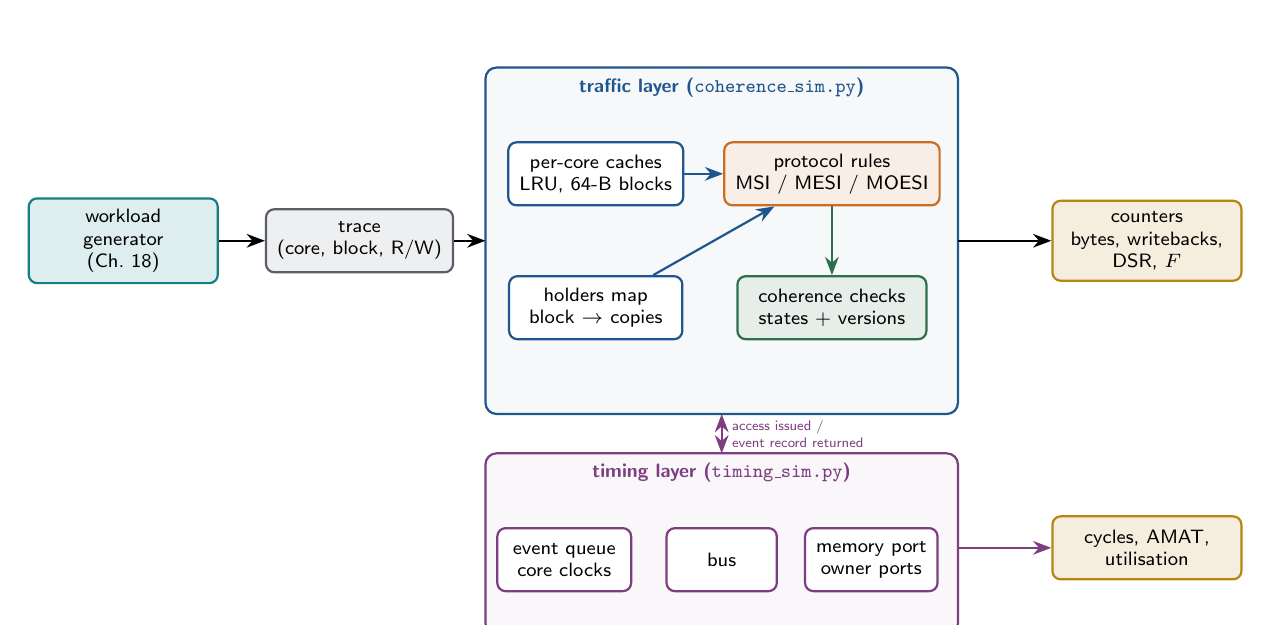
\begin{tikzpicture}[font=\sffamily\scriptsize,
    bx/.style={draw, thick, rounded corners=3pt, minimum height=0.8cm, align=center, inner sep=4pt},
    ar/.style={-{Stealth}, thick}]
  \node[bx, fill=tealC!14, draw=tealC, minimum width=2.4cm] (gen) at (0,0) {workload\\generator\\(Ch.~18)};
  \node[bx, fill=coreGrey!10, draw=coreGrey, minimum width=2.0cm] (tr) at (3.0,0) {trace\\(core, block, R/W)};
  \draw[thick, mesiBlue, rounded corners=4pt, fill=mesiBlue!4] (4.6,-2.2) rectangle (10.6,2.2);
  \node[font=\sffamily\bfseries\scriptsize, text=mesiBlue] at (7.6,1.95) {traffic layer (\texttt{coherence\_sim.py})};
  \node[bx, fill=white, draw=mesiBlue, minimum width=2.2cm] (cache) at (6.0,0.85) {per-core caches\\LRU, 64-B blocks};
  \node[bx, fill=white, draw=mesiBlue, minimum width=2.2cm] (hold) at (6.0,-0.85) {holders map\\block $\to$ copies};
  \node[bx, fill=moesiOrange!12, draw=moesiOrange, minimum width=2.4cm] (rules) at (9.0,0.85) {protocol rules\\MSI / MESI / MOESI};
  \node[bx, fill=memGreen!12, draw=memGreen, minimum width=2.4cm] (chk) at (9.0,-0.85) {coherence checks\\states + versions};
  \draw[ar, mesiBlue] (cache) -- (rules); \draw[ar, mesiBlue] (hold) -- (rules);
  \draw[ar, memGreen] (rules) -- (chk);
  \draw[thick, plumC, rounded corners=4pt, fill=plumC!4] (4.6,-5.0) rectangle (10.6,-2.7);
  \node[font=\sffamily\bfseries\scriptsize, text=plumC] at (7.6,-2.95) {timing layer (\texttt{timing\_sim.py})};
  \node[bx, fill=white, draw=plumC, minimum width=1.7cm] (q) at (5.6,-4.05) {event queue\\core clocks};
  \node[bx, fill=white, draw=plumC, minimum width=1.4cm] (bus) at (7.6,-4.05) {bus};
  \node[bx, fill=white, draw=plumC, minimum width=1.5cm] (mp) at (9.5,-4.05) {memory port\\owner ports};
  \node[bx, fill=amberC!14, draw=amberC, minimum width=2.4cm] (out) at (13.0,0) {counters\\bytes, writebacks,\\DSR, $F$};
  \node[bx, fill=amberC!14, draw=amberC, minimum width=2.4cm] (out2) at (13.0,-3.9) {cycles, AMAT,\\utilisation};
  \draw[ar] (gen) -- (tr); \draw[ar] (tr) -- (4.6,0);
  \draw[ar] (10.6,0) -- (out);
  \draw[ar, plumC] (10.6,-3.9) -- (out2);
  \draw[ar, plumC, {Stealth}-{Stealth}] (7.6,-2.2) -- node[right, font=\sffamily\tiny, align=left]{access issued /\\event record returned} (7.6,-2.7);
\end{tikzpicture}
\end{bigfig}
\caption[Simulator architecture]{The two layers. The traffic layer is the protocol:
it decides states, messages and bytes. The timing layer decides when accesses
happen and how long they take, from the event record returned for each access.}
\label{fig:sim-arch}
\end{figure}

% ---------------------------------------------------------------
\section{The Traffic Layer}
\label{sec:sim-traffic}
\sectionmap{[Traffic layer [Data structures] [Rules as code]
  [Byte accounting] [Event record]]}
\index{MESI}\index{MOESI}\index{MSI}\index{Owned state}\index{Exclusive state}\index{forced writeback}\index{snooping protocol}\index{LRU replacement}\index{owner}\index{simulator!timing layer}%

Each core's cache is an ordered dictionary from block number to a small record of
state and version. The dictionary order is the LRU order, so a hit moves the block
to the end and the victim in a full cache is the first entry. A second dictionary,
the holders map, records which cores hold each block and points at the same
records, so a snoop (``does any other cache hold this block, and in what state?'')
is one lookup instead of a search of every cache. Two more maps hold each block's
latest version and the version last written back, for the value checks of \cref{sec:method-correct}, and counters record every quantity of \cref{tab:metrics}.

The three protocols share one class, and two flags, ``has \stE'' and ``has \stO'',
select MSI, MESI or MOESI. With both flags set the rules are exactly those of
\cref{tab:transition-diff}. The read handler (\cref{lst:readmiss} in
\cref{app:code}) holds the only rule that separates MESI from MOESI on a remote
read: when another cache holds the block in \stM\ or \stO, the code either charges
a control and a data message and relabels the holder \stO\ (MOESI), or also charges
a writeback, updates memory's version and relabels the holder \stS\ (MSI and MESI).
One rule was not fixed by earlier chapters: a write miss to a block that another
cache holds dirty. The simulator moves the block from the dirty owner to the
writer, invalidates every other copy and writes nothing to memory, since the writer
becomes the new dirty owner. It does this the same way in all three protocols, so
it cannot favour either side, and none of the four sharing patterns of
\cref{tab:traffic-patterns} uses it, so it does not affect the analytical numbers
the simulator is checked against.

Every action is priced with the constants of \cref{tab:counting-rules}, written
once at the top of the source file so the simulator and the report cannot disagree
(\cref{tab:sim-bytes}). At the end of a run each block still in \stM\ or \stO\ is
charged one writeback (the drain), so a protocol cannot look cheaper by leaving
writebacks unpaid when measurement stops. Before each access the layer clears a
four-field event record and fills it as the rules run: the kind of access (hit,
read miss, write miss or upgrade), the supplier (a core, or memory), whether a
forced writeback happened, and whether a dirty block was evicted. The timing layer
reads only this record and never needs the protocol rules. Adding the record
changed no counter; the traffic results were byte-for-byte identical before and
after.

\begin{table}[htbp]
\centering
\caption{Bytes charged by the traffic layer for each action (interconnect /
memory).}
\label{tab:sim-bytes}
\small
\begin{tabular}{@{}L{6.6cm} c c c@{}}
\toprule
Action & MSI & MESI & MOESI \\
\midrule
Read miss served by memory & 80 / 0 & 80 / 0 & 80 / 0 \\
Read miss, block in \stM\ elsewhere & 152 / 64 & 152 / 64 & 80 / 0 \\
Read miss, block in \stO\ elsewhere & --- & --- & 80 / 0 \\
Write miss (any supplier) & 80 / 0 & 80 / 0 & 80 / 0 \\
Upgrade (write hit in \stS, or \stO) & 8 / 0 & 8 / 0 & 8 / 0 \\
Write hit in \stE & --- & 0 / 0 & 0 / 0 \\
Eviction of \stM\ (or \stO) & 72 / 64 & 72 / 64 & 72 / 64 \\
Drain: block still dirty at the end & 72 / 64 & 72 / 64 & 72 / 64 \\
\bottomrule
\end{tabular}
\end{table}

% ---------------------------------------------------------------
\section{The Timing Layer}
\label{sec:sim-timing}
\label{sec:sim-example}
\sectionmap{[Timing layer [Latencies from the report] [Three kinds of resource]
  [Event loop] [Serial or overlapped write back] [Two readers at once]]}
\index{MESI}\index{MOESI}\index{forced writeback}\index{snooping protocol}\index{bus utilisation}\index{owner}\index{simulator!traffic layer}\index{simulator!timing layer}%

The timing layer uses the latencies the report has already assumed and adds as few
as possible (\cref{tab:sim-latency}). Each added parameter is varied in at least one
experiment of Chapter~18, so no conclusion rests on one guessed value. Chapter~8
defined $T_{\mathrm{coh}}$ as the time to get a block from another cache
``including any writeback the protocol performs on the way'', which fits MESI's
dirty read. MOESI makes no writeback on the same read, so its latency is
$T_{\mathrm{coh}}$ minus the writeback transfer time, 51 cycles on the assumed bus.
This is the smallest change to the report's numbers that lets the two protocols
differ in latency at all.

\begin{table}[htbp]
\centering
\caption{Parameters of the timing layer. The upper block repeats the report's own
assumptions; the lower blocks are introduced or derived here.}
\label{tab:sim-latency}
\small
\begin{tabular}{@{}L{1.9cm} r L{5.6cm} L{3.4cm}@{}}
\toprule
Symbol & Value & Meaning & Source \\
\midrule
$T_{L1}$ & 1 & cache hit (cycles) & \cref{eq:amat}, Sarangi Ex.~147 \\
$T_{\mathrm{mem}}$ & 100 & read served by memory & \cref{eq:amat}, \cref{fig:hierarchy} \\
$T_{\mathrm{coh}}$ & 60 & read served by a modified copy, including the writeback & \cref{eq:amat-coh}, \cref{fig:amat-bars} \\
--- & --- & one message on the bus at a time; requests queue & \cref{eq:util} \\
\midrule
bus width & 8\,B/cycle & a 72-B message takes 9 cycles & assumed; Ch.~18 E1 \\
arbitration & 1 & cycles per message & assumed \\
$T_{\mathrm{upg}}$ & 10 & upgrade / invalidation round trip & assumed \\
$M_{\mathrm{occ}}$ & 10 & memory port busy per 64-B access & assumed; swept in E5 \\
$O_{\mathrm{occ}}$ & 10 & owner's cache port busy per block supplied & assumed; swept in E4 \\
think & 2--2000 & mean cycles of computation between memory operations & swept in E1 \\
\midrule
$t_{\mathrm{wb}}$ & 9 & writeback transfer: $\lceil 72/8 \rceil$ & derived \\
$T_{\mathrm{c2c}}$ & 51 & cache-to-cache read without writeback: $T_{\mathrm{coh}} - t_{\mathrm{wb}}$ & derived; swept in E4 \\
\bottomrule
\end{tabular}
\end{table}

Three kinds of shared resource are modelled, each serving one request at a time in
arrival order (\cref{fig:sim-resources}). The bus is held by each message for
$\lceil\text{bytes}/8\rceil + 1$ cycles, 2 for a control message and 10 for a data
or writeback message, so a MESI dirty read holds it for $2+10+10=22$ cycles and the
same read under MOESI for 12. The memory port is held for $M_{\mathrm{occ}}$ cycles
by each 64-byte read or write, including every forced writeback. Each core's cache
port is held for $O_{\mathrm{occ}}$ cycles whenever that core supplies a block as an
owner. The bus is split-transaction: it is busy only while messages are on it, not
while memory fetches the data. A dirty eviction is posted, so it occupies the bus
and memory port without stalling the core.

\begin{figure}[htbp]
\centering
\begin{bigfig}[0.9]
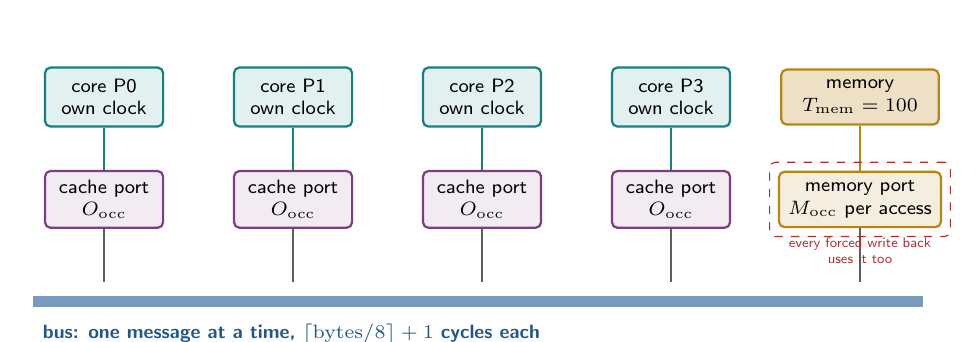
\begin{tikzpicture}[font=\sffamily\scriptsize,
    core/.style={draw, thick, rounded corners=2pt, minimum width=1.5cm, minimum height=0.75cm, align=center},
    res/.style={draw, thick, rounded corners=2pt, minimum height=0.7cm, align=center},
    ar/.style={-{Stealth}, thick}]
  \foreach \i/\x in {0/0, 1/2.4, 2/4.8, 3/7.2} {
    \node[core, fill=tealC!12, draw=tealC] (c\i) at (\x,2.6) {core P\i\\own clock};
    \node[res, fill=plumC!10, draw=plumC, minimum width=1.5cm] (p\i) at (\x,1.3) {cache port\\$O_{\mathrm{occ}}$};
    \draw[thick, tealC] (c\i) -- (p\i);
    \draw[thick, coreGrey] (p\i.south) -- (\x,0.25);
  }
  \draw[line width=4pt, mesiBlue!60] (-0.9,0) -- (10.4,0);
  \node[font=\sffamily\bfseries\scriptsize, text=mesiBlue, anchor=west] at (-0.9,-0.4) {bus: one message at a time, $\lceil \mathrm{bytes}/8\rceil + 1$ cycles each};
  \node[res, fill=amberC!14, draw=amberC, minimum width=2.0cm] (mp) at (9.6,1.3) {memory port\\$M_{\mathrm{occ}}$ per access};
  \node[res, fill=amberC!25, draw=amberC, minimum width=2.0cm] (mem) at (9.6,2.6) {memory\\$T_{\mathrm{mem}} = 100$};
  \draw[thick, amberC] (mem) -- (mp); \draw[thick, coreGrey] (mp.south) -- (9.6,0.25);
  \node[draw=alertRed, dashed, rounded corners=2pt, fit=(mp), inner sep=3pt] {};
  \node[text=alertRed, font=\sffamily\tiny, align=center] at (9.6,0.65) {every forced write back\\uses it too};
\end{tikzpicture}
\end{bigfig}
\caption[Timing-layer resources]{Each core has its own clock and a cache port used
when it supplies data as an owner; all cores share one bus and one memory port. A
request waits while the resource it needs is busy.}
\label{fig:sim-resources}
\end{figure}

The layer is a discrete-event simulation. Each core's accesses form a stream, and
between accesses the core computes for a think time drawn from an exponential
distribution. The draws come from a seed that depends only on the core and the
configuration, so the MESI and MOESI runs see identical think times. A priority
queue holds each core's next ready time. The loop takes the earliest core, lets the
traffic layer process its access, and charges the access: a
hit costs $T_{L1}$; a miss waits for and occupies the bus, then waits for the memory
port (memory supplies) or the owner's port (a cache supplies) and completes after
$T_{\mathrm{mem}}$, $T_{\mathrm{coh}}$ or $T_{\mathrm{c2c}}$; an upgrade completes
after $T_{\mathrm{upg}}$. The core's next access is ready when this one completes
plus the next think time. \Cref{lst:timing} in \cref{app:code} is the code that
charges a miss.

Whether the reader of a modified block waits for the forced writeback depends on
the bus, not the protocol. On some buses memory captures the flushed block as it
passes to the reader, so one transfer serves both; on others the writeback is a
separate step. The report's $T_{\mathrm{coh}}$, which includes the writeback,
implies the second. The timing layer supports both (\cref{fig:sim-wbmode}). In the
serial mode, the default, the reader waits $T_{\mathrm{coh}}=60$ cycles. In the
overlapped mode it waits $T_{\mathrm{c2c}}=51$, and the writeback occupies the bus
and memory port without delaying it. Part~VI reports both.

\begin{figure}[htbp]
\centering
\begin{bigfig}[0.95]
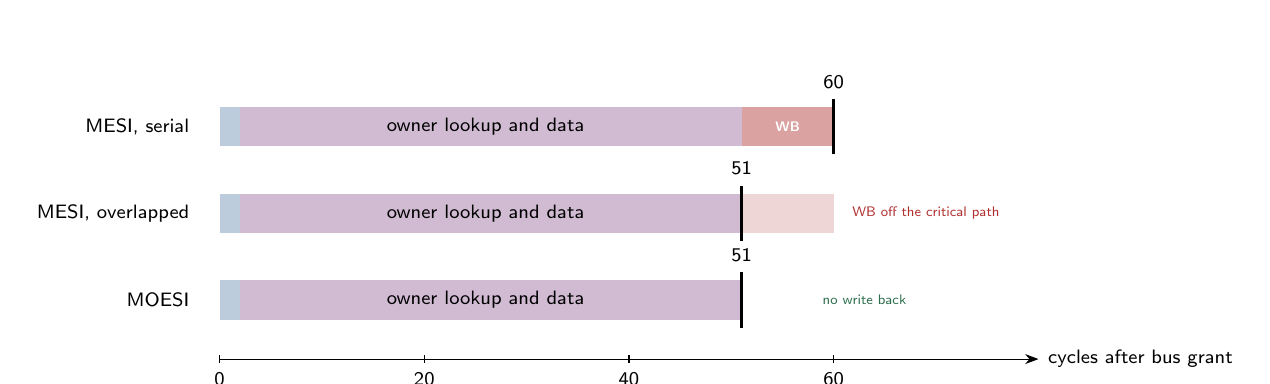
\begin{tikzpicture}[font=\sffamily\scriptsize, x=0.13cm]
  \foreach \y/\l in {0/{MESI, serial}, -1.1/{MESI, overlapped}, -2.2/{MOESI}} {
    \node[anchor=east] at (-2,\y) {\l};
  }
  \fill[mesiBlue!30] (0,-0.25) rectangle (2,0.25);
  \fill[plumC!35] (2,-0.25) rectangle (51,0.25);
  \fill[alertRed!45] (51,-0.25) rectangle (60,0.25);
  \node at (26,0) {owner lookup and data};
  \node[text=white, font=\sffamily\bfseries\tiny] at (55.5,0) {WB};
  \draw[very thick] (60,-0.35) -- (60,0.35) node[above]{60};
  \fill[mesiBlue!30] (0,-1.35) rectangle (2,-0.85);
  \fill[plumC!35] (2,-1.35) rectangle (51,-0.85);
  \fill[alertRed!20] (51,-1.35) rectangle (60,-0.85);
  \node at (26,-1.1) {owner lookup and data};
  \node[font=\sffamily\tiny, text=alertRed] at (69,-1.1) {WB off the critical path};
  \draw[very thick] (51,-1.45) -- (51,-0.75) node[above]{51};
  \fill[mesiBlue!30] (0,-2.45) rectangle (2,-1.95);
  \fill[plumC!35] (2,-2.45) rectangle (51,-1.95);
  \node at (26,-2.2) {owner lookup and data};
  \node[font=\sffamily\tiny, text=memGreen] at (63,-2.2) {no write back};
  \draw[very thick] (51,-2.55) -- (51,-1.85) node[above]{51};
  \draw[-{Stealth}] (0,-2.95) -- (80,-2.95) node[right]{cycles after bus grant};
  \foreach \x in {0,20,40,60} { \draw (\x,-2.9) -- (\x,-3.0) node[below]{\x}; }
\end{tikzpicture}
\end{bigfig}
\caption[Serial and overlapped writeback]{Latency of a read served by a modified
copy on an idle system. In serial mode the MESI reader waits for the 9-cycle
writeback; in overlapped mode it does not, but the writeback still uses the bus and
memory port. MOESI makes no writeback.}
\label{fig:sim-wbmode}
\end{figure}

On an idle system the latencies differ by 9 cycles, but waiting changes this.
Suppose P0 holds blocks A and B in \stM, and at the same moment P1 reads A and P2
reads B. Both need the bus, so one waits for the other. \Cref{fig:sim-gantt} and
\cref{tab:sim-gantt} trace the two reads in serial mode; the simulator gives exactly
these values. The first reader gains the 9 cycles of the writeback, as in
\cref{eq:dL}. The second gains 19: its own 9 plus the 10 cycles it no longer waits
for the first reader's writeback to clear the bus. With more cores competing, every
waiting request gains the same way, which is why H2 expects the time gain to grow
with utilisation.

\begin{figure}[htbp]
\centering
\begin{bigfig}[0.95]
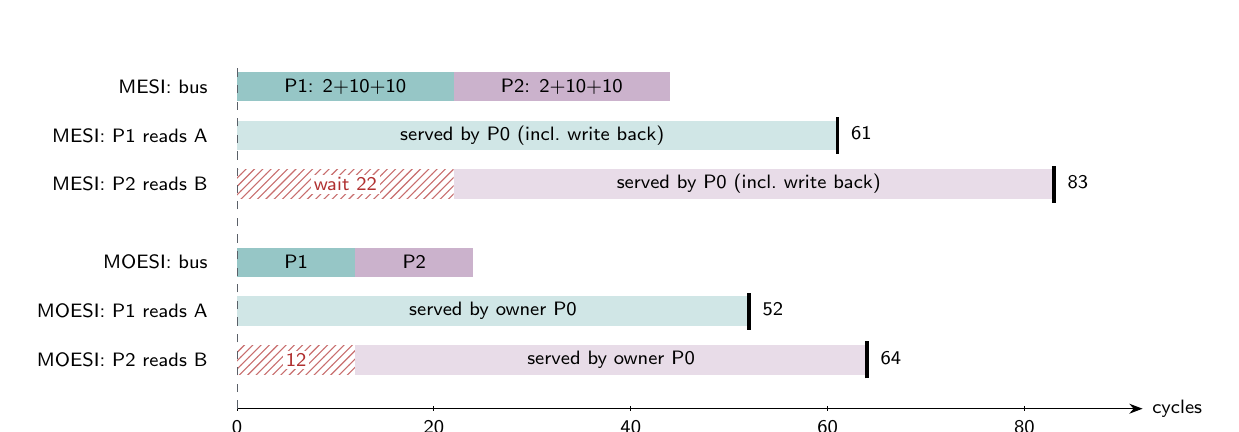
\begin{tikzpicture}[font=\sffamily\scriptsize, x=0.125cm, y=0.62cm]
  \def\row#1#2{\node[anchor=east] at (-2,#1) {#2};}
  \row{0}{MESI: bus}
  \row{-1}{MESI: P1 reads A}
  \row{-2}{MESI: P2 reads B}
  \row{-3.6}{MOESI: bus}
  \row{-4.6}{MOESI: P1 reads A}
  \row{-5.6}{MOESI: P2 reads B}
  \fill[tealC!45] (0,-0.3) rectangle (22,0.3);  \node at (11,0) {P1: 2+10+10};
  \fill[plumC!40] (22,-0.3) rectangle (44,0.3); \node at (33,0) {P2: 2+10+10};
  \fill[tealC!20] (0,-1.3) rectangle (61,-0.7); \node at (30,-1) {served by P0 (incl.\ write back)};
  \draw[very thick] (61,-1.38) -- (61,-0.62) node[right, xshift=1pt, yshift=-6pt]{61};
  \fill[pattern=north east lines, pattern color=alertRed!70] (0,-2.3) rectangle (22,-1.7);
  \node[text=alertRed, fill=white, inner sep=1pt] at (11,-2) {wait 22};
  \fill[plumC!18] (22,-2.3) rectangle (83,-1.7); \node at (52,-2) {served by P0 (incl.\ write back)};
  \draw[very thick] (83,-2.38) -- (83,-1.62) node[right, xshift=1pt, yshift=-6pt]{83};
  \fill[tealC!45] (0,-3.9) rectangle (12,-3.3);  \node at (6,-3.6) {P1};
  \fill[plumC!40] (12,-3.9) rectangle (24,-3.3); \node at (18,-3.6) {P2};
  \fill[tealC!20] (0,-4.9) rectangle (52,-4.3); \node at (26,-4.6) {served by owner P0};
  \draw[very thick] (52,-4.98) -- (52,-4.22) node[right, xshift=1pt, yshift=-6pt]{52};
  \fill[pattern=north east lines, pattern color=alertRed!70] (0,-5.9) rectangle (12,-5.3);
  \node[text=alertRed, fill=white, inner sep=1pt] at (6,-5.6) {12};
  \fill[plumC!18] (12,-5.9) rectangle (64,-5.3); \node at (38,-5.6) {served by owner P0};
  \draw[very thick] (64,-5.98) -- (64,-5.22) node[right, xshift=1pt, yshift=-6pt]{64};
  \draw[-{Stealth}] (0,-6.6) -- (92,-6.6) node[right]{cycles};
  \foreach \x in {0,20,40,60,80} { \draw (\x,-6.55) -- (\x,-6.65) node[below]{\x}; }
  \draw[dashed, coreGrey] (0,-6.6) -- (0,0.4);
\end{tikzpicture}
\end{bigfig}
\caption[Two simultaneous dirty reads]{Two simultaneous reads of blocks held in \stM\
by P0 (serial mode). Under MESI each read holds the bus for 22 cycles because of the
writeback, so P2 waits 22 cycles; under MOESI it waits 12. Latencies include
$T_{L1}=1$.}
\label{fig:sim-gantt}
\end{figure}

\begin{table}[htbp]
\centering
\caption{The example of \cref{fig:sim-gantt} in numbers (cycles).}
\label{tab:sim-gantt}
\small
\begin{tabular}{@{}l c c c c@{}}
\toprule
 & P1 latency & P2 latency & Mean latency & Bus busy for the two reads \\
\midrule
MESI (serial) & 61 & 83 & 72 & 44 \\
MOESI & 52 & 64 & 58 & 24 \\
\midrule
MOESI saving & 9 & 19 & 14 (19\,\%) & 20 (45\,\%) \\
\bottomrule
\end{tabular}
\end{table}

The layer has no processor pipeline (a core stalls fully on a miss), no out-of-order
execution or prefetching, no DRAM banks or row buffers, one level of private cache,
and one snooping bus instead of a network. Execution time is the finish time of the
slowest core. These simplifications are why Part~VI compares MESI with MOESI
relative to each other on identical inputs and makes no claim about absolute run
times.

% ---------------------------------------------------------------
\section{Verification}
\label{sec:sim-verify}
\sectionmap{[Verification [Every analytical number reproduced] [Coherence checked on random runs]
  [Part IV identities hold] [Timing checks] [Only then results]]}
\index{simulator!traffic layer}\index{simulator!timing layer}\index{verification}%

We verified the simulator in four automated ways before taking any result from it;
the commands in \cref{lst:repro} (\cref{app:code}) rerun all of them in seconds.
First, the traffic layer was run on the pattern kernels of Chapter~18 and its byte
counts compared with the numbers derived by hand in Parts~II and~III
(\cref{tab:verify-patterns}); all 22 checks match exactly. Steady-state values are
measured as the difference between runs of $k+1$ and $k$ units, which cancels the
cold start and the drain.

\begin{table}[htbp]
\centering
\caption{Verification against \cref{tab:traffic-patterns} ($C=1$) and against
\cref{eq:upd-mesi,eq:upd-moesi} (bytes per round with $C$ consumers). Each cell of
the upper block is simulated\,/\,analytical bytes.}
\label{tab:verify-patterns}
\label{tab:verify-bc}
\small
\begin{tabular}{@{}l c c c c@{}}
\toprule
Pattern (unit) & MSI & MESI & MOESI & Result \\
\midrule
Private (read, write, evict) & 160 / 160 & 152 / 152 & 152 / 152 & 3 of 3 match \\
Read-only (per reader) & 80 / 80 & 80 / 80 & 80 / 80 & 3 of 3 match \\
Producer--consumer (per round) & 160 / 160 & 160 / 160 & 88 / 88 & 3 of 3 match \\
Migratory (per hand-off) & 160 / 160 & 160 / 160 & 88 / 88 & 3 of 3 match \\
\midrule
\multicolumn{5}{@{}L{12.4cm}@{}}{Producer--consumer with $C = 1, 2, 4, 8, 15$
  consumers: MESI simulated 160, 240, 400, 720, 1280\,B, equal to $160+80(C-1)$;
  MOESI simulated 88, 168, 328, 648, 1208\,B, equal to $88+80(C-1)$. 10 of 10
  match.} \\
\bottomrule
\end{tabular}
\end{table}

Second, the kernels exercise few transitions, so the layer was also run with every
check of \cref{sec:method-correct} enabled on 144 random workloads: every
combination of 2, 4, 8 and 16 cores, cache capacities of 2, 4 and 16 blocks and
unlimited, three sharing mixes and all three protocols, with 20\,000 accesses each.
The tiny caches force constant evictions of owned blocks, the case most likely to
expose a missing writeback. No state or value invariant was violated.

Third, the propositions of Part~IV were derived by hand, so the simulator checks
them and they check the simulator (\cref{tab:verify-identities}). Each held exactly,
to floating-point rounding, on all 468 paired runs of the two traffic experiments.
Fourth, the timing layer was checked against latencies worked out by hand on an
idle system and on one case with deliberate queueing (\cref{tab:verify-timing}); all
eleven checks pass.

\begin{table}[htbp]
\centering
\caption{The results of Part~IV checked on every paired traffic run (468 pairs).}
\label{tab:verify-identities}
\small
\begin{tabular}{@{}L{5.3cm} L{4.6cm} l@{}}
\toprule
Statement & Check on each pair & Result \\
\midrule
\Cref{prop:residency}: same contents & equal read misses, write misses,
  upgrades and hit rates & held in all pairs \\
\Cref{eq:dB-writebacks}: only writebacks differ & $\Delta B = 72\,(W_{\mathrm{MESI}} - W_{\mathrm{MOESI}})$ & held in all pairs \\
Forced writebacks are dirty reads & $B_{\mathrm{fwb}} = 72\,n_{\mathrm{dr}}$ under MESI & held in all pairs \\
\Cref{prop:never-worse}: bounds & $0 \le \Delta B \le 72\,n_{\mathrm{dr}}$ & held in all pairs \\
\Cref{eq:identity}: saving identity & $|S_B - \sigma\cdot72\,\dsr/\bar b| < 10^{-15}$ & held in all pairs \\
\bottomrule
\end{tabular}
\end{table}

\begin{table}[htbp]
\centering
\caption{Verification of the timing layer (cycles; latencies include $T_{L1}=1$).}
\label{tab:verify-timing}
\small
\begin{tabular}{@{}L{7.0cm} r r l@{}}
\toprule
Check & Simulated & Expected & \\
\midrule
Read miss served by memory & 101 & 101 & pass \\
MESI: two memory misses then an upgrade (sum) & 213 & 213 & pass \\
MESI serial: write miss + dirty read (sum) & 162 & 162 & pass \\
MOESI: write miss + dirty read (sum) & 153 & 153 & pass \\
MESI overlapped: write miss + dirty read (sum) & 153 & 153 & pass \\
Two simultaneous misses: mean latency & 107 & 107 & pass \\
Two simultaneous misses: mean bus wait & 6 & 6 & pass \\
Derived $T_{\mathrm{c2c}} = T_{\mathrm{coh}} - 9$ & 51 & 51 & pass \\
Bus cycles of a control and a data message & 2, 10 & 2, 10 & pass \\
MESI bus-busy cycles: write miss + dirty read & 34 & 34 & pass \\
MOESI bus-busy cycles: write miss + dirty read & 24 & 24 & pass \\
\bottomrule
\end{tabular}
\end{table}

% ===============================================================
%  Chapter 18 -- Workloads, Configurations and Metrics
% ===============================================================
\chapter{Workloads, Configurations and Metrics}
\label{ch:workloads}

\begin{figure}[htbp]
\centering
\adjustbox{max width=\linewidth}{%
\begin{forest}
  chapter map,
  [Chapter 18
    [Scope [Planned vs used] [What is lost]]
    [Kernels {\&} mixtures [Four micro-traces] [Knob $d$] [Seeds]]
    [Experiments [Traffic: 2 sweeps] [Timing: E1 to E5]]
    [Metrics {\&} reproducibility [Traffic] [Time]]
  ]
\end{forest}}
\caption[]{Structure of Chapter~18: the workloads, the
experiments that use them, and how every reported number is defined.}
\label{fig:ch18-map}
\end{figure}

% ---------------------------------------------------------------
\section{From the Problem Scope to the Workloads}
\label{sec:wl-scope}
\sectionmap{[Scope [Chapter 10 planned OpenMP and directories]
  [Used: synthetic patterns on a bus] [Why] [What is lost]]}
\index{MESI}\index{MOESI}\index{directory protocol}\index{OpenMP}%

\Cref{tab:scope-change} compares the scope set in \cref{sec:prob-scope} with what
the study uses. The changes have one cause. The method of Chapter~15 needs a
simulator in which MESI and MOESI differ only in three rules, and we chose to build
it rather than adapt a large external one. Running real programs would have meant
turning them into traces with an instrumentation tool we did not have time to set
up and validate, so we generated the four sharing patterns directly, since
Chapter~9 showed they decide the forced-writeback cost.

\begin{table}[htbp]
\centering
\caption{Scope planned in Chapter 10 and scope used in this study.}
\label{tab:scope-change}
\small
\begin{tabular}{@{}L{2.6cm} L{4.2cm} L{5.8cm}@{}}
\toprule
Item & Planned (\cref{sec:prob-scope}) & Used, and consequence \\
\midrule
Workloads & OpenMP C programs (e.g.\ matrix multiplication, image filtering) &
  synthetic traces of the four sharing patterns; results describe the patterns,
  not named programs \\
Organisation & snooping bus and directory & snooping bus only; directory
  results remain analytical (\cref{tab:p2p}) \\
Simulator & trace-driven, checked with \texttt{gem5} & our two-layer simulator;
  no cycle-accurate cross-check \\
Congestion metric & network-on-chip congestion & bus utilisation and queueing
  delay on the snooping bus (\cref{fig:res-h2}); no network-on-chip model \\
Cores & 2, 4, 8, 16 & 2, 4, 8, 16 (unchanged) \\
Protocols & MSI family & MSI, MESI, MOESI (unchanged) \\
Consistency, false sharing & out of scope & out of scope (unchanged) \\
\bottomrule
\end{tabular}
\end{table}

% ---------------------------------------------------------------
\section{Pattern Kernels and Synthetic Mixtures}
\label{sec:wl-kernels}
\label{sec:wl-mixtures}
\sectionmap{[Workloads [Four kernels for verification] [Four address pools]
  [One knob d for dirty sharing] [Fixed seeds]]}
\index{dirty sharing}\index{Dirty Sharing Ratio}\index{sharing patterns!producer--consumer}\index{sharing patterns!migratory}\index{verification}%

Four short deterministic traces reproduce one unit of each sharing pattern of
\cref{tab:patterns} on one block (\cref{fig:kernels}). They are used for
verification, and their names are reused for the pools of the synthetic generator.

\begin{figure}[htbp]
\centering
\begin{bigfig}[0.92]
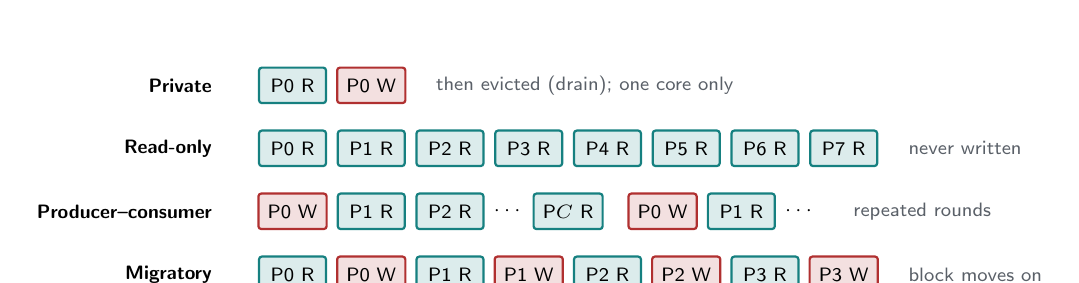
\begin{tikzpicture}[font=\sffamily\scriptsize,
    rd/.style={draw=tealC, fill=tealC!15, thick, rounded corners=1pt, minimum width=0.85cm, minimum height=0.45cm},
    wr/.style={draw=alertRed, fill=alertRed!15, thick, rounded corners=1pt, minimum width=0.85cm, minimum height=0.45cm}]
  \node[anchor=east, font=\sffamily\bfseries\scriptsize] at (-0.3,0) {Private};
  \node[rd] at (0.6,0) {P0 R}; \node[wr] at (1.6,0) {P0 W};
  \node[anchor=west, text=coreGrey] at (2.3,0) {then evicted (drain); one core only};
  \node[anchor=east, font=\sffamily\bfseries\scriptsize] at (-0.3,-0.8) {Read-only};
  \foreach \i in {0,...,7} { \node[rd] at (0.6+\i*1.0,-0.8) {P\i\ R}; }
  \node[anchor=west, text=coreGrey] at (8.3,-0.8) {never written};
  \node[anchor=east, font=\sffamily\bfseries\scriptsize] at (-0.3,-1.6) {Producer--consumer};
  \node[wr] at (0.6,-1.6) {P0 W}; \node[rd] at (1.6,-1.6) {P1 R}; \node[rd] at (2.6,-1.6) {P2 R};
  \node at (3.35,-1.6) {$\cdots$}; \node[rd] at (4.1,-1.6) {P$C$ R};
  \node[wr] at (5.3,-1.6) {P0 W}; \node[rd] at (6.3,-1.6) {P1 R}; \node at (7.05,-1.6) {$\cdots$};
  \node[anchor=west, text=coreGrey] at (7.6,-1.6) {repeated rounds};
  \node[anchor=east, font=\sffamily\bfseries\scriptsize] at (-0.3,-2.4) {Migratory};
  \foreach \i/\c in {0/0,1/1,2/2,3/3} {
    \node[rd] at (0.6+\i*2.0,-2.4) {P\c\ R}; \node[wr] at (1.6+\i*2.0,-2.4) {P\c\ W}; }
  \node[anchor=west, text=coreGrey] at (8.3,-2.4) {block moves on};
\end{tikzpicture}
\end{bigfig}
\caption[The four pattern kernels]{The four pattern kernels, each on one block (R:
read, W: write). Steady-state costs come from differencing runs of $k+1$ and $k$
units.}
\label{fig:kernels}
\end{figure}

Programs mix the patterns, so the experiments use traces that mix them in
controlled proportions. The generator splits the address space into four pools
(\cref{fig:addr-pools}) and builds a trace one operation at a time. It picks a pool
with probability $(1-d)/2$ for private, $(1-d)/2$ for read-only, $d/2$ for
producer--consumer and $d/2$ for migratory, so $d$ is the share of operations in
the dirty-sharing patterns. A private operation is a random core accessing one of
its own 96 blocks, writing with probability 0.3. A read-only operation is a random
core reading one of 24 shared blocks. A producer--consumer operation picks one of 24
blocks, each with a fixed producer (block number modulo $N$); with probability
$p_w$ the producer writes it, and otherwise a random other core reads it. A
migratory operation has a core different from the last one read and then write one
of 12 blocks. The knob $d$ sets the input, and the DSR is measured. Because DSR is
weighted by transactions (\cref{eq:dsr-mix}) it rises steeply at small $d$, so the
sweeps use values of $d$ concentrated near zero. Every random choice is seeded by
the configuration, so a trace can be regenerated exactly (\cref{tab:wl-params}).

\begin{figure}[htbp]
\centering
\begin{bigfig}[0.9]
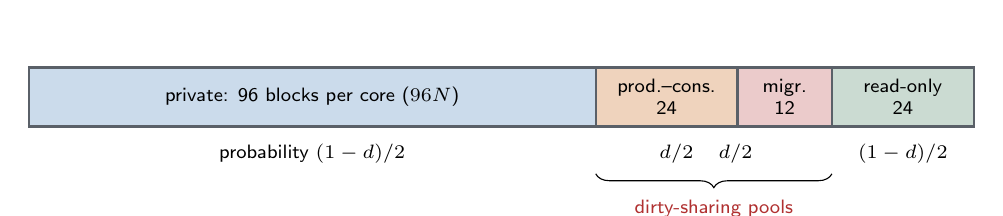
\begin{tikzpicture}[font=\sffamily\scriptsize]
  \def\h{0.75}
  \fill[skyC!25] (0,0) rectangle (7.2,\h);   \node at (3.6,\h/2) {private: 96 blocks per core ($96N$)};
  \fill[moesiOrange!30] (7.2,0) rectangle (9.0,\h); \node[align=center] at (8.1,\h/2) {prod.--cons.\\24};
  \fill[alertRed!25] (9.0,0) rectangle (10.2,\h); \node[align=center] at (9.6,\h/2) {migr.\\12};
  \fill[memGreen!25] (10.2,0) rectangle (12.0,\h); \node[align=center] at (11.1,\h/2) {read-only\\24};
  \draw[thick, coreGrey] (0,0) rectangle (12.0,\h);
  \foreach \x in {7.2,9.0,10.2} { \draw[thick, coreGrey] (\x,0) -- (\x,\h); }
  \node[anchor=north] at (3.6,-0.1) {probability $(1-d)/2$};
  \node[anchor=north, align=center] at (8.6,-0.1) {$d/2$ \;\; $d/2$};
  \node[anchor=north] at (11.1,-0.1) {$(1-d)/2$};
  \draw[decorate, decoration={brace, amplitude=5pt, mirror}] (7.2,-0.6) -- (10.2,-0.6)
     node[midway, below=6pt, text=alertRed]{dirty-sharing pools};
\end{tikzpicture}
\end{bigfig}
\caption[Address pools of the generator]{The generator's address space and the
probability of each pool. Only the two middle pools can produce dirty reads.}
\label{fig:addr-pools}
\end{figure}

\begin{table}[htbp]
\centering
\caption{Parameters of the workload generator.}
\label{tab:wl-params}
\small
\begin{tabular}{@{}L{3.6cm} L{3.6cm} L{5.4cm}@{}}
\toprule
Parameter & Values & Role \\
\midrule
Cores $N$ & 2, 4, 8, 16 & one stream per core \\
Dirty-sharing share $d$ & 0 to 1 (11 values, most below 0.1) & share of operations in the producer--consumer and migratory pools \\
Producer write probability $p_w$ & 0.15, 0.3, 0.5 & writes per round of producer--consumer sharing \\
Private write probability & 0.3 & writes to private data \\
Pool sizes & 96 per core / 24 / 12 / 24 blocks & private / prod.--cons. / migratory / read-only \\
Trace length & 60\,000 (traffic), 30\,000 (timing) & accesses per run \\
Seeds & 1, 2, 3 & three independent traces per configuration \\
\bottomrule
\end{tabular}
\end{table}

% ---------------------------------------------------------------
\section{Experiments, Metrics and Reproducibility}
\label{sec:wl-experiments}
\label{sec:wl-metrics}
\label{sec:wl-repro}
\sectionmap{[Experiments [{T1, T2 traffic}] [E1 to E5 timing]
  [Metrics defined once] [All paired] [About one minute to rerun]]}
\index{simulator!traffic layer}\index{simulator!timing layer}%

\Cref{tab:experiments} lists every experiment reported in Part~VI. Each
configuration runs under each protocol on the same trace, as Chapter~15 requires,
giving 468 paired traffic runs and 288 paired timing runs; the last column names
the hypothesis each experiment tests. \Cref{tab:metrics} defines every number
Part~VI reports. Traffic metrics come from the traffic layer and time metrics from
the timing layer, and protocols are always compared per pair (\cref{eq:paired}). The
code, inputs and outputs are kept together, and every number in Part~VI can be
regenerated with the commands in \cref{lst:repro} on any machine with Python~3.9 or
later and \texttt{numpy}, \texttt{pandas} and \texttt{matplotlib}. Seeds are fixed,
so repeated runs give byte-identical result files; we checked this for both layers.

\begin{table}[htbp]
\centering
\caption{Experiments. ``Fixed'' values hold unless the row varies them. Caches are
1024 blocks (64\,KB) unless varied, large enough for the private pool.}
\label{tab:experiments}
\small
\begin{tabular}{@{}l L{3.0cm} L{4.6cm} c L{2.0cm}@{}}
\toprule
 & Varies & Fixed & Pairs & Tests \\
\midrule
T1 & $N$, $d$ (11), $p_w$ (3), seed (3) & 64\,KB caches; MSI, MESI, MOESI & 396 & H1, H3, H4 \\
T2 & cache 4--1024 blocks, $d \in\{0.2,0.5,0.8\}$, seed & $N=8$, $p_w = 0.3$ & 72 & H3, H4 ($\sigma$) \\
\midrule
E1 & think 2--2000 cycles (10), $N \in\{8,16\}$, writeback mode & $d=0.5$, $p_w=0.3$ & 120 & H2 \\
E2 & $N$ (4), think $\in\{40, 300\}$ & $d=0.5$, $p_w=0.3$ & 24 & H1, H2 \\
E3 & cache 4--1024 blocks, $d \in\{0.2,0.5,0.8\}$ & $N=8$, think 40 & 72 & H4 \\
E4 & $T_{\mathrm{coh}}$ 30--200, $O_{\mathrm{occ}}$ 5--40 & $N=8$, $d=0.5$, think 40 & 60 & H4 (Effect B) \\
E5 & $M_{\mathrm{occ}}$ 5--40 & $N=8$, $d=0.5$, think 40 & 12 & H2 (memory) \\
\bottomrule
\multicolumn{5}{@{}l}{\footnotesize T = traffic layer only (trace order); E = both layers. All rows use 3 seeds.}
\end{tabular}
\end{table}

\begin{table}[htbp]
\centering
\caption{Metrics reported in Part~VI.}
\label{tab:metrics}
\small
\begin{tabular}{@{}L{2.4cm} L{6.4cm} L{3.8cm}@{}}
\toprule
Metric & Definition & Defined in \\
\midrule
$B_{\mathrm{tot}}$ & interconnect bytes, including the drain & \cref{tab:sim-bytes} \\
$B_{\mathrm{fwb}}$ & bytes of forced writebacks (MESI, MSI) & \cref{sec:prob-formal} \\
$F$ & $B_{\mathrm{fwb}}/B_{\mathrm{tot}}$ under MESI & \cref{eq:fwb-fraction} \\
$\dsr$ & dirty reads / coherence transactions, under MESI & \cref{sec:dsr-def} \\
$\bar b$ & $B_{\mathrm{tot}}/n_{\mathrm{tx}}$ under MESI & \cref{eq:identity} \\
$\sigma$ & saved epochs / dirty reads & \cref{eq:sigma} \\
$S_B$ & $1 - B_{\mathrm{tot}}(\mathrm{MOESI})/B_{\mathrm{tot}}(\mathrm{MESI})$ & \cref{eq:paired} \\
Memory bytes & bytes written to memory & \cref{tab:sim-bytes} \\
\midrule
$T$ & finish time of the slowest core (cycles) & \cref{sec:sim-timing} \\
AMAT & mean cycles per memory operation, hits included & \cref{eq:amat-coh} \\
$U_{\mathrm{bus}}$, $U_{\mathrm{mem}}$ & busy cycles / $T$ for bus and memory port & \cref{eq:util} \\
Speed-up & $T(\mathrm{MESI})/T(\mathrm{MOESI})$ & \cref{eq:paired} \\
Time reduction & $1 - T(\mathrm{MOESI})/T(\mathrm{MESI})$ & --- \\
Dirty-read latency & mean latency of reads served by a modified or owned copy & \cref{eq:dL} \\
\bottomrule
\end{tabular}
\end{table}

% ===============================================================
%  PART VI -- Results and Discussion (Chapters 19--20)
%  Every number in this Part comes from the simulator of Part V.
%  Plotted data: data/*.dat, written by simulator/make_report_data.py
% ===============================================================

\newtcolorbox{verdictbox}[2][memGreen]{
  colback=#1!6, colframe=#1, coltitle=white,
  colbacktitle=#1, fonttitle=\sffamily\bfseries\small,
  title={#2}, boxrule=0.6pt, arc=2pt, fontupper=\small,
  left=6pt, right=6pt, top=4pt, bottom=4pt
}

\part{Results and Discussion}
\label{part:results}

\begin{center}
\adjustbox{max width=\linewidth}{%
\begin{forest}
  part map,
  [Part VI
    [Ch.~19: Traffic {\&} Time
      [H1: $F$ and cores] [Traffic saved] [H2: bytes to time] [AMAT] [Memory bandwidth]]
    [Ch.~20: Testing the Predictor
      [Input knob vs DSR] [H3: DSR predicts the saving] [Survival fraction] [H4: when MOESI loses] [Verdicts]]
  ]
\end{forest}}
\end{center}

\begin{keybox}[What Part VI does]
Part~VI reports what the simulator measured and judges each hypothesis of
\cref{tab:hypotheses} against it. Chapter~19 covers cost: the size of the
forced-writeback fraction from 2 to 16 cores (H1), the traffic MOESI removes, and
whether removed traffic becomes saved time (H2). Chapter~20 tests the Dirty Sharing
Ratio as a predictor (H3) and looks for conditions under which MOESI does worse
than MESI (H4). Each section ends with a verdict: held, partly held or failed.
Unless stated otherwise a number is the mean over three seeds of paired runs
(\cref{eq:paired}), ``points'' means percentage points, and the experiments are
those of \cref{tab:experiments}.
\end{keybox}

% ===============================================================
%  Chapter 19 -- Traffic, Execution Time and AMAT
% ===============================================================
\chapter{Traffic, Execution Time and AMAT from 2 to 16 Cores}
\label{ch:res-traffic}
\index{AMAT}%

\begin{figure}[htbp]
\centering
\adjustbox{max width=\linewidth}{%
\begin{forest}
  chapter map,
  [Chapter 19
    [H1: $F$ and cores [Falls at every mix] [More readers per epoch]]
    [Traffic saved [Never more bytes] [Memory writes cut]]
    [H2: bytes to time [Gain follows utilisation] [Saturation limit]]
    [AMAT {\&} memory [AMAT is not time] [Memory-bound gains most]]
  ]
\end{forest}}
\caption[]{Structure of Chapter~19: the cost of forced
writebacks (H1), the traffic MOESI removes, and how much of it becomes time (H2).}
\label{fig:ch19-map}
\end{figure}

% ---------------------------------------------------------------
\section{H1: The Forced-Writeback Fraction from 2 to 16 Cores}
\label{sec:res-h1}
\sectionmap{[H1 [{F at 2, 4, 8, 16 cores}] [Falls at every sharing mix]
  [{Why: more readers per epoch}] [Verdict: held]]}
\index{MESI}\index{forced writeback}\index{dirty sharing}\index{dirty epoch}\index{sharing patterns!producer--consumer}\index{sharing patterns!migratory}%

H1 predicted that, for a fixed sharing structure, $F(W,N)$ falls as cores are added,
because each forced writeback is shared among more read misses.
\Cref{fig:res-h1}(a) plots $F$ under MESI against the core count for four mixes, from
almost no dirty sharing ($d=0.005$) to nothing else ($d=1$). Every line falls. The
fall is steepest when sharing is light: at $d=0.005$, $F$ drops from 17.5\,\% at 2
cores to 3.7\,\% at 16, almost a factor of five, while at $d=1$ it drops only from
44.9 to 39.0\,\%. \Cref{tab:res-h1} gives the numbers for workloads with
$d\ge0.1$, where dirty sharing is a large part of the traffic.

\begin{figure}[htbp]
\centering
\begin{bigfig}[1.0]
\begin{tikzpicture}
  \begin{axis}[name=a, width=7.4cm, height=5.6cm,
      title={\sffamily\small (a) Forced-writeback fraction $F$},
      xlabel={Cores $N$}, ylabel={$F$ under MESI (\%)},
      xmode=log, log basis x=2, xtick={2,4,8,16}, xticklabels={2,4,8,16},
      ymin=0, ymax=50, grid=major, grid style={coreGrey!15},
      label style={font=\small}, tick label style={font=\scriptsize},
      legend style={at={(1.08,-0.28)}, anchor=north, legend columns=4, font=\scriptsize, draw=none}]
    \addplot[very thick, tealC, mark=*] table[x=N, y=d0p005] {data/h1_F_vs_N.dat}; \addlegendentry{$d = 0.005$}
    \addplot[very thick, plumC, mark=square*] table[x=N, y=d0p02] {data/h1_F_vs_N.dat}; \addlegendentry{$d = 0.02$}
    \addplot[very thick, amberC, mark=triangle*] table[x=N, y=d0p1] {data/h1_F_vs_N.dat}; \addlegendentry{$d = 0.1$}
    \addplot[very thick, brickC, mark=diamond*] table[x=N, y=d1] {data/h1_F_vs_N.dat}; \addlegendentry{$d = 1$}
  \end{axis}
  \begin{axis}[at={(a.east)}, anchor=west, xshift=1.5cm, width=7.4cm, height=5.6cm,
      title={\sffamily\small (b) Read misses served by a modified copy},
      xlabel={Cores $N$}, ylabel={share of read misses (\%)},
      xmode=log, log basis x=2, xtick={2,4,8,16}, xticklabels={2,4,8,16},
      ymin=0, ymax=105, grid=major, grid style={coreGrey!15},
      label style={font=\small}, tick label style={font=\scriptsize}]
    \addplot[very thick, tealC, mark=*] table[x=N, y=d0p005] {data/h1_dirtyshare_vs_N.dat};
    \addplot[very thick, plumC, mark=square*] table[x=N, y=d0p02] {data/h1_dirtyshare_vs_N.dat};
    \addplot[very thick, amberC, mark=triangle*] table[x=N, y=d0p1] {data/h1_dirtyshare_vs_N.dat};
    \addplot[very thick, brickC, mark=diamond*] table[x=N, y=d1] {data/h1_dirtyshare_vs_N.dat};
  \end{axis}
\end{tikzpicture}
\end{bigfig}
\caption[H1: forced-writeback fraction against cores]{Experiment T1. (a) The
forced-writeback fraction falls with the core count at every mix. (b) With more
cores a smaller share of read misses finds the block modified, because the first
reader of each epoch has already forced the writeback that cleans it for the rest.
Means over seeds and producer write probabilities.}
\label{fig:res-h1}
\end{figure}

\begin{table}[htbp]
\centering
\caption{H1 in numbers: workloads with $d \ge 0.1$ (36 runs per core count).
``Dirty share'' is the fraction of read misses served by a modified copy.}
\label{tab:res-h1}
\small
\begin{tabular}{@{}c c c c c c c@{}}
\toprule
Cores & Mean $F$ (\%) & Min $F$ & Max $F$ & Dirty share (\%) & $\dsr$ & $\bar b$ (B) \\
\midrule
2 & 43.6 & 41.8 & 44.9 & 97.3 & 0.491 & 81.1 \\
4 & 40.0 & 36.8 & 42.9 & 84.4 & 0.454 & 81.8 \\
8 & 36.8 & 31.3 & 41.8 & 75.1 & 0.423 & 83.1 \\
16 & 33.4 & 25.4 & 41.4 & 67.5 & 0.393 & 85.3 \\
\bottomrule
\end{tabular}
\end{table}

\Cref{fig:res-h1}(b) shows the mechanism proposed in Chapter~16. With two cores, a
read miss on shared data can only find the block in the one other cache, the
writer, so 97\,\% of read misses on such data are dirty reads and nearly all of
them carry a forced writeback. With sixteen cores, the first reader in an epoch
forces the writeback and the readers after it find a clean block in memory, so only
67.5\,\% of read misses are dirty reads. The writeback stays at 72 bytes per epoch,
but it is shared among more 80-byte read misses, so its share falls, exactly as
$F=72/B(C)$ in \cref{eq:pc-model} falls with more consumers. Producers that write
more often create more epochs and so raise $F$: at 16 cores, $F$ rises from 31.6 to
35.3\,\% as the producer write probability goes from 0.15 to 0.5. The largest value
measured, 44.9\,\%, is the steady-state 72/160 of one producer--consumer or
migratory hand-off (\cref{tab:dsr-patterns}), and the measured range of 25 to
45\,\% for $d\ge0.1$ lies inside the 10 to 45\,\% derived in Chapter~10.

\begin{verdictbox}{Verdict on H1: held}
At every mix $F$ falls steadily from 2 to 16 cores, for the predicted reason. When
dirty sharing is substantial, the forced writeback is a third to nearly half of
MESI's coherence traffic (33.4 to 43.6\,\% on average).
\end{verdictbox}

% ---------------------------------------------------------------
\section{Traffic Saved by MOESI}
\label{sec:res-traffic}
\sectionmap{[Traffic [Never more bytes than MESI] [MESI never more than MSI]
  [Memory writes cut much more] [Growth with dirty sharing]]}
\index{MESI}\index{MOESI}\index{MSI}\index{Exclusive state}\index{forced writeback}\index{dirty sharing}%

\Cref{fig:res-traffic} compares the three protocols at 8 cores for four mixes, and
\cref{tab:res-traffic} averages over all core counts. In all 468 paired traffic
runs, including the 72 with caches as small as four blocks, MOESI moved no more
bytes than MESI, as \cref{prop:never-worse} requires. The saving tracks $F$
closely, within one point in every row of the table; Chapter~20 explains what this
does and does not show. MESI in turn never moved more bytes than MSI, and up to
3.5\,\% fewer (3.24\,\% on average with no dirty sharing). That is the \stE\ saving
of \cref{sec:fam-mesi}: a private block read and then written needs no upgrade in
MESI. It shrinks to zero as dirty sharing takes over, since shared blocks are never
in \stE.

\begin{figure}[htbp]
\centering
\begin{bigfig}[1.0]
\begin{tikzpicture}
  \begin{axis}[name=a, ybar, bar width=8pt, width=7.6cm, height=5.6cm,
      title={\sffamily\small (a) Interconnect bytes (MSI $=100$)},
      xlabel={dirty-sharing share $d$}, ylabel={relative bytes},
      xtick={0,1,2,3}, xticklabels={0.005, 0.02, 0.1, 0.5},
      ymin=0, ymax=118, enlarge x limits=0.18, grid=major, grid style={coreGrey!15},
      label style={font=\small}, tick label style={font=\scriptsize},
      legend style={at={(1.08,-0.28)}, anchor=north, legend columns=3, font=\scriptsize, draw=none}]
    \addplot[fill=coreGrey!45, draw=coreGrey] table[x=x, y=msi] {data/traffic_n8.dat}; \addlegendentry{MSI}
    \addplot[fill=mesiBlue!70, draw=mesiBlue] table[x=x, y=mesi] {data/traffic_n8.dat}; \addlegendentry{MESI}
    \addplot[fill=moesiOrange!75, draw=moesiOrange] table[x=x, y=moesi] {data/traffic_n8.dat}; \addlegendentry{MOESI}
  \end{axis}
  \begin{axis}[at={(a.east)}, anchor=west, xshift=1.5cm, ybar, bar width=10pt, width=7.6cm, height=5.6cm,
      title={\sffamily\small (b) Bytes written to memory (MESI $=100$)},
      xlabel={dirty-sharing share $d$}, ylabel={relative bytes},
      xtick={0,1,2,3}, xticklabels={0.005, 0.02, 0.1, 0.5},
      ymin=0, ymax=118, enlarge x limits=0.18, grid=major, grid style={coreGrey!15},
      label style={font=\small}, tick label style={font=\scriptsize},
      nodes near coords, nodes near coords style={font=\tiny, /pgf/number format/fixed, /pgf/number format/precision=0}]
    \addplot[fill=mesiBlue!70, draw=mesiBlue] table[x=x, y=memmesi] {data/traffic_n8.dat};
    \addplot[fill=moesiOrange!75, draw=moesiOrange] table[x=x, y=memmoesi] {data/traffic_n8.dat};
  \end{axis}
\end{tikzpicture}
\end{bigfig}
\caption[Traffic of the three protocols]{Experiment T1 at 8 cores. (a) MESI moves
slightly fewer bytes than MSI (the \stE\ state), and MOESI many fewer as dirty
sharing grows. (b) At $d=0.1$ MOESI writes less than a fifth of what MESI writes to
memory. MSI writes the same bytes to memory as MESI.}
\label{fig:res-traffic}
\end{figure}

\begin{table}[htbp]
\centering
\caption{Traffic results of experiment T1 for selected dirty-sharing shares,
averaged over 2 to 16 cores (36 runs per row).}
\label{tab:res-traffic}
\small
\begin{tabular}{@{}c c c c c@{}}
\toprule
 & & \multicolumn{2}{c}{MOESI saves vs MESI (\%)} & MESI saves \\
\cmidrule(lr){3-4}
$d$ & $F$ (\%) & interconnect bytes & memory writes & vs MSI (\%) \\
\midrule
0 & 0.0 & 0.0 & --- & 3.24 \\
0.001 & 1.7 & 1.6 & 3.8 & 3.07 \\
0.005 & 9.8 & 9.1 & 21.9 & 2.43 \\
0.01 & 16.0 & 15.3 & 36.7 & 1.98 \\
0.02 & 22.6 & 22.1 & 52.7 & 1.47 \\
0.05 & 30.5 & 30.2 & 71.9 & 0.86 \\
0.1 & 34.8 & 34.6 & 82.8 & 0.53 \\
0.5 & 39.7 & 39.7 & 95.3 & 0.14 \\
1 & 41.6 & 41.5 & 99.8 & 0.00 \\
\bottomrule
\end{tabular}
\end{table}

Memory sees most of the benefit. MOESI's cut in memory writes is about 2.4 times
its cut in interconnect bytes in every row. In these workloads the private data
fits in the caches and is rarely evicted, so almost every MESI memory write is a
forced writeback, and removing forced writebacks removes most memory writes:
82.8\,\% at $d=0.1$ and 99.8\,\% at $d=1$. Whether that saves time depends on
whether memory is a bottleneck (\cref{sec:res-memory}).

% ---------------------------------------------------------------
\section{H2: From Traffic to Execution Time}
\label{sec:res-h2}
\sectionmap{[H2 [Load sweep E1] [Gain follows utilisation]
  [Queueing explains it] [Saturation limit confirmed] [Verdict: held]]}
\index{MESI}\index{MOESI}\index{forced writeback}\index{bus utilisation}\index{Effect A and Effect B}%

H2 predicted that MOESI's time gain is near zero at low bus utilisation and rises
towards the ratio of bus-busy times, $C_{\mathrm{bus}}(\mathrm{MESI}) /
C_{\mathrm{bus}}(\mathrm{MOESI})$ (\cref{eq:sat-limit}), as utilisation nears
100\,\%. Experiment E1 keeps the workload fixed ($d=0.5$) and changes only how long
each core computes between memory operations, from 2000 cycles (an idle bus) to 2
(a saturated one). \Cref{fig:res-h2}(a) plots the time reduction against MESI's bus
utilisation, and \cref{tab:res-h2} gives the 8-core numbers.

\begin{figure}[htbp]
\centering
\begin{bigfig}[1.0]
\begin{tikzpicture}
  \begin{axis}[name=a, width=7.4cm, height=5.6cm,
      title={\sffamily\small (a) Time saved by MOESI},
      xlabel={MESI bus utilisation (\%)}, ylabel={execution-time reduction (\%)},
      xmin=0, xmax=100, ymin=0, ymax=31, grid=major, grid style={coreGrey!15},
      label style={font=\small}, tick label style={font=\scriptsize},
      legend style={at={(0.03,0.97)}, anchor=north west, font=\scriptsize, draw=none, fill=white, fill opacity=0.8, text opacity=1}]
    \addplot[very thick, mesiBlue, mark=*] table[x=Um, y=red] {data/e1_serial_N8.dat}; \addlegendentry{$N=8$, serial}
    \addplot[very thick, mesiBlue, dashed, mark=o] table[x=Um, y=red] {data/e1_overlap_N8.dat}; \addlegendentry{$N=8$, overlapped}
    \addplot[very thick, moesiOrange, mark=square*] table[x=Um, y=red] {data/e1_serial_N16.dat}; \addlegendentry{$N=16$, serial}
    \addplot[very thick, moesiOrange, dashed, mark=square] table[x=Um, y=red] {data/e1_overlap_N16.dat}; \addlegendentry{$N=16$, overlapped}
  \end{axis}
  \begin{axis}[at={(a.east)}, anchor=west, xshift=2.2cm, width=7.4cm, height=5.6cm,
      title={\sffamily\small (b) Waiting for the bus},
      xlabel={bus utilisation of that protocol (\%)}, ylabel={mean wait per transaction (cycles)},
      xmin=0, xmax=100, ymode=log, ymin=0.05, ymax=200, grid=major, grid style={coreGrey!15},
      label style={font=\small}, tick label style={font=\scriptsize},
      legend style={at={(0.03,0.97)}, anchor=north west, font=\scriptsize, draw=none, fill=white, fill opacity=0.8, text opacity=1}]
    \addplot[very thick, mesiBlue, mark=*] table[x=Um, y=Wm] {data/e1_serial_N8.dat}; \addlegendentry{MESI, $N=8$}
    \addplot[very thick, moesiOrange, mark=square*] table[x=Uo, y=Wo] {data/e1_serial_N8.dat}; \addlegendentry{MOESI, $N=8$}
    \addplot[thick, mesiBlue!60, dashed, mark=o] table[x=Um, y=Wm] {data/e1_serial_N16.dat}; \addlegendentry{MESI, $N=16$}
    \addplot[thick, moesiOrange!70, dashed, mark=square] table[x=Uo, y=Wo] {data/e1_serial_N16.dat}; \addlegendentry{MOESI, $N=16$}
  \end{axis}
\end{tikzpicture}
\end{bigfig}
\caption[H2: time saved against bus utilisation]{Experiment E1. (a) MOESI's time
gain is negligible on a lightly used bus and grows steeply as the bus fills.
(b) Waiting grows sharply with utilisation and both protocols lie on one curve;
MOESI sits further left because each of its dirty reads holds the bus for 12 cycles
instead of 22. Mean of three seeds, $d=0.5$.}
\label{fig:res-h2}
\end{figure}

\begin{table}[htbp]
\centering
\caption{Experiment E1 at 8 cores, serial writeback. ``Converted'' is the share of
the byte saving that appears as time saving. The last two columns compare the
speed-up with the limit of \cref{eq:sat-limit}.}
\label{tab:res-h2}
\small
\begin{tabular}{@{}r c c c c c c c@{}}
\toprule
Think & \multicolumn{2}{c}{Bus utilisation (\%)} & Bytes saved & Time saved & Converted & Speed-up & $C_{\mathrm{bus}}$ ratio \\
\cmidrule(lr){2-3}
(cycles) & MESI & MOESI & (\%) & (\%) & (\%) & & \\
\midrule
2000 & 2.5 & 1.7 & 32.6 & 0.3 & 1 & 1.003 & 1.459 \\
600 & 8.1 & 5.6 & 32.6 & 0.9 & 3 & 1.009 & 1.458 \\
300 & 15.5 & 10.8 & 32.4 & 1.8 & 6 & 1.019 & 1.454 \\
150 & 28.5 & 20.4 & 32.3 & 3.7 & 11 & 1.039 & 1.452 \\
80 & 46.2 & 34.3 & 31.9 & 6.8 & 21 & 1.073 & 1.445 \\
40 & 69.3 & 55.4 & 31.3 & 12.6 & 40 & 1.144 & 1.432 \\
20 & 87.0 & 77.1 & 30.8 & 20.7 & 67 & 1.260 & 1.422 \\
10 & 95.4 & 91.3 & 30.2 & 25.9 & 86 & 1.350 & 1.411 \\
5 & 98.0 & 96.8 & 30.0 & 28.0 & 93 & 1.388 & 1.406 \\
2 & 98.9 & 98.3 & 29.7 & 28.2 & 95 & 1.393 & 1.402 \\
\bottomrule
\end{tabular}
\end{table}

MOESI removes about 30\,\% of the bytes at every load, yet the time it saves ranges
from 0.3 to 28.2\,\%. Below 35\,\% bus utilisation it saves at most 3.7\,\% of the
time at 8 cores and 2.4\,\% at 16; above 65\,\% it saves 12.6 to 28.2\,\%. Put
another way, about 1\,\% of the saved bytes turn into saved time on an idle bus and
95\,\% on a saturated one. \Cref{fig:res-h2}(b) shows why. The mean wait for the bus
grows from a fraction of a cycle at low utilisation to tens of cycles near
100\,\%, as \cref{eq:util} suggests, and MESI and MOESI lie on the same curve, so
neither waits less at a given utilisation. MOESI wins because it does the same work
at a lower utilisation. At 8 cores with 40 cycles of computation, MESI's bus is
69\,\% busy and a transaction waits 11.0 cycles on average, while MOESI's is 55\,\%
busy and waits 4.6. On an idle bus there is no waiting to remove, and the only gain
left is the 9-cycle writeback of each dirty read (Effect~A of
\cref{fig:two-effects}), which is tiny next to the computation.

The last two columns of \cref{tab:res-h2} confirm the saturation limit of
\cref{eq:sat-limit}: a speed-up of 1.393 against a bus-busy ratio of 1.402 at 8
cores, and 1.318 against 1.319 at 16. At low load the ratio is still about 1.46,
since MOESI keeps the bus a third less busy, but the speed-up is 1.003. Whether the
MESI reader waits for the writeback (\cref{fig:sim-wbmode}) matters little: at 8
cores and moderate load MOESI saves 12.6\,\% of the time in serial mode and 11.0\,\%
in overlapped mode, and both reach 28.2\,\% at saturation. The forced writeback
costs time mainly through the bus time it takes up, not through the latency it adds
to one read. The 16-core curves rise at lighter per-core loads than the 8-core
ones, because twice the cores reach saturation at half the per-core demand
(\cref{eq:util}).

\begin{verdictbox}{Verdict on H2: held}
Saved traffic becomes saved time in proportion to how busy the bus is: about 1\,\%
of the byte saving at 2.5\,\% utilisation, 40\,\% at 69\,\% and 95\,\% at
saturation, where the speed-up reaches the bus-occupancy limit. A comparison run on
a lightly loaded system will see almost no difference in time, however many bytes
are saved.
\end{verdictbox}

% ---------------------------------------------------------------
\section{AMAT, Scaling with Cores and Memory Bandwidth}
\label{sec:res-amat}
\label{sec:res-memory}
\sectionmap{[AMAT and memory [Experiment E2] [Idle latencies match the report]
  [AMAT is not execution time] [E5: memory-bound gains most]]}
\index{MESI}\index{MOESI}\index{forced writeback}\index{Dirty Sharing Ratio}\index{dirty epoch}\index{AMAT}\index{bus utilisation}\index{owner}\index{Effect A and Effect B}%

Experiment E2 runs the same workload on 2 to 16 cores at a light and a heavy load
(\cref{fig:res-amat,tab:res-amat}). On a lightly loaded bus with two cores a dirty
read takes 61.1 cycles under MESI and 52.0 under MOESI, within a fraction of a
cycle of $T_{L1}+T_{\mathrm{coh}}=61$ and $T_{L1}+T_{\mathrm{c2c}}=52$
(\cref{tab:sim-latency}). As cores and load grow, queueing adds to both and more to
MESI: at 16 cores under heavy load a dirty read takes 125.5 cycles under MESI and
86.6 under MOESI.

\begin{figure}[htbp]
\centering
\begin{minipage}[c]{0.52\linewidth}\centering
\begin{tikzpicture}
  \begin{axis}[width=\linewidth, height=5.4cm,
      xlabel={Cores $N$}, ylabel={measured AMAT (cycles)},
      xmode=log, log basis x=2, xtick={2,4,8,16}, xticklabels={2,4,8,16},
      ymin=0, ymax=85, grid=major, grid style={coreGrey!15},
      label style={font=\footnotesize}, tick label style={font=\scriptsize},
      legend style={at={(0.03,0.97)}, anchor=north west, font=\tiny, draw=none, fill=white}]
    \addplot[very thick, mesiBlue, mark=*] table[x=N, y=Am] {data/e2_heavy.dat}; \addlegendentry{MESI, heavy (think 40)}
    \addplot[very thick, moesiOrange, mark=square*] table[x=N, y=Ao] {data/e2_heavy.dat}; \addlegendentry{MOESI, heavy}
    \addplot[thick, dashed, mesiBlue, mark=o] table[x=N, y=Am] {data/e2_light.dat}; \addlegendentry{MESI, light (think 300)}
    \addplot[thick, dashed, moesiOrange, mark=square] table[x=N, y=Ao] {data/e2_light.dat}; \addlegendentry{MOESI, light}
  \end{axis}
\end{tikzpicture}
\caption[AMAT against cores]{Experiment E2: AMAT grows with cores and the MESI--MOESI
gap widens as the bus gets busier. $d=0.5$.}
\label{fig:res-amat}
\end{minipage}\hfill
\begin{minipage}[c]{0.45\linewidth}\centering
\begin{tikzpicture}
  \begin{axis}[ybar, bar width=7pt, width=\linewidth, height=5.4cm,
      xlabel={memory-port occupancy (cycles)},
      ylabel={memory-port utilisation (\%)},
      xtick={0,1,2,3}, xticklabels={5,10,20,40},
      ymin=0, ymax=125, enlarge x limits=0.15, grid=major, grid style={coreGrey!15},
      label style={font=\footnotesize}, tick label style={font=\scriptsize},
      legend style={at={(0.03,0.97)}, anchor=north west, font=\tiny, draw=none, fill=white}]
    \addplot[fill=mesiBlue!70, draw=mesiBlue] table[x=x, y=MUm] {data/e5_memport.dat}; \addlegendentry{MESI}
    \addplot[fill=moesiOrange!75, draw=moesiOrange] table[x=x, y=MUo] {data/e5_memport.dat}; \addlegendentry{MOESI}
    \node[font=\tiny, text=memGreen!70!black] at (axis cs:0,28) {$-12.6\%$};
    \node[font=\tiny, text=memGreen!70!black] at (axis cs:1,45) {$-12.6\%$};
    \node[font=\tiny, text=memGreen!70!black] at (axis cs:2,78) {$-13.6\%$};
    \node[font=\tiny\bfseries, text=memGreen!70!black] at (axis cs:3,109) {$-35.9\%$};
  \end{axis}
\end{tikzpicture}
\caption[Memory-port utilisation]{Experiment E5 (8 cores, think 40, $d=0.5$):
memory-port use, with MOESI's time reduction above each pair.}
\label{fig:res-memory}
\end{minipage}
\end{figure}

\begin{table}[htbp]
\centering
\caption{Experiment E2: AMAT and dirty-read latency (cycles), with the
execution-time reduction for comparison.}
\label{tab:res-amat}
\small
\begin{tabular}{@{}l c c c c c c c c@{}}
\toprule
Load & $N$ & Bus util. & \multicolumn{3}{c}{AMAT} &
  \multicolumn{2}{c}{Dirty-read latency} & Time \\
\cmidrule(lr){4-6}\cmidrule(lr){7-8}
 & & MESI (\%) & MESI & MOESI & cut (\%) & MESI & MOESI & cut (\%) \\
\midrule
light & 2 & 2.8 & 14.4 & 12.8 & 11.2 & 61.1 & 52.0 & 0.5 \\
light & 4 & 7.1 & 22.3 & 18.1 & 18.7 & 61.5 & 52.2 & 1.3 \\
light & 8 & 15.5 & 29.0 & 22.6 & 21.9 & 62.4 & 52.6 & 1.8 \\
light & 16 & 32.5 & 37.6 & 28.7 & 23.7 & 64.7 & 53.8 & 2.4 \\
\midrule
heavy & 2 & 15.7 & 14.5 & 12.9 & 11.2 & 61.8 & 52.3 & 3.0 \\
heavy & 4 & 35.8 & 23.8 & 18.8 & 21.1 & 64.0 & 53.2 & 8.0 \\
heavy & 8 & 69.3 & 35.0 & 25.2 & 27.9 & 71.2 & 56.5 & 12.6 \\
heavy & 16 & 97.0 & 78.6 & 50.2 & 36.0 & 125.5 & 86.6 & 23.8 \\
\bottomrule
\end{tabular}
\end{table}

MOESI lowers AMAT by 11 to 36\,\%, far more than it lowers execution time (0.5 to
23.8\,\%). AMAT averages memory operations only, while execution time also includes
the computation between them, which dominates at light load. And part of the AMAT
cut is Effect~B of \cref{fig:two-effects}: under MOESI the readers after the first
in each epoch are served by the owner in 51 cycles instead of by memory in 100. The
example of \cref{tab:amat-compare} counted Effect~A alone and predicted an AMAT cut
below 10\,\%; the measured cut is larger because of Effect~B. This is why
Chapter~16 kept the two effects apart: only Effect~A is the forced writeback.

Experiment E5 varies how long the memory port is busy per 64-byte access, from 5
cycles (fast memory) to 40 (slow memory) (\cref{fig:res-memory}). With fast memory
the bus is the bottleneck and MOESI saves the same 12.6\,\% as in E1. The memory
port, though, is 17 to 98\,\% busy under MESI across the four settings and 2 to
16\,\% under MOESI, because every forced writeback is also a memory write. At 40
cycles per access MESI saturates the port (98\,\% busy), requests queue at memory,
the bus sits idle half the time (its utilisation falls from 69 to 50\,\%), and
MOESI, which hardly uses the port, finishes 35.9\,\% sooner. This is the
memory-bandwidth argument of Chapter~9 in numbers: the forced writeback costs time
wherever bandwidth is scarce, on the bus or at memory.

% ===============================================================
%  Chapter 20 -- Testing the Dirty Sharing Ratio
% ===============================================================
\chapter{Testing the Dirty Sharing Ratio}
\label{ch:res-dsr}
\index{Dirty Sharing Ratio}%

\begin{figure}[htbp]
\centering
\adjustbox{max width=\linewidth}{%
\begin{forest}
  chapter map,
  [Chapter 20
    [Why not the input knob [$d$ is far from linear]]
    [H3: DSR as predictor [One straight line] [Three cross-checks]]
    [Survival {\&} small caches [$\sigma$ stays near 1] [DSR carries the effect]]
    [H4: when MOESI loses [Never in bytes] [Slow cache-to-cache]]
    [What it means [Published studies] [Design rule] [Verdicts]]
  ]
\end{forest}}
\caption[]{Structure of Chapter~20: why a measured ratio is
needed, how well DSR predicts MOESI's saving, what small caches do, and when MOESI
is slower than MESI.}
\label{fig:ch20-map}
\end{figure}

% ---------------------------------------------------------------
\section{Why the Input Knob Is Not a Predictor}
\label{sec:res-knob}
\sectionmap{[Input knob [d describes the program] [Saving saturates in d]
  [{Same d, different savings}] [Need a measured ratio]]}

The generator's knob $d$, the share of operations that touch dirty-shared data, is
the obvious measure of how much a program shares, so we checked it first
(\cref{fig:res-knob}). The curve is far from straight: the saving rises fast at
small $d$ and levels off near 40\,\%, so the correlation between $d$ and the saving
is only 0.64 (0.93 with $d$ on a log scale). At a given $d$ the saving also depends
strongly on the core count, and at $d=0.1$ single runs range from 25.2 to 42.0\,\%.
Both problems have the cause found in \cref{sec:dsr-patterns}: what matters is how
many transactions the shared accesses produce, not how many accesses there are
(\cref{eq:dsr-mix}).

\begin{figure}[htbp]
\centering
\begin{tikzpicture}
  \begin{axis}[width=10cm, height=5.2cm,
      xlabel={dirty-sharing share of operations, $d$ (log scale)}, ylabel={MOESI saving $S_B$ (\%)},
      xmode=log, xmin=0.0008, xmax=1.2, ymin=0, ymax=48, grid=major, grid style={coreGrey!15},
      label style={font=\small}, tick label style={font=\scriptsize},
      legend style={at={(0.03,0.97)}, anchor=north west, font=\scriptsize, draw=none, fill=white}]
    \addplot[very thick, skyC, mark=*] table[x=d, y=N2] {data/S_vs_d.dat}; \addlegendentry{$N=2$}
    \addplot[very thick, leafC, mark=square*] table[x=d, y=N4] {data/S_vs_d.dat}; \addlegendentry{$N=4$}
    \addplot[very thick, amberC, mark=triangle*] table[x=d, y=N8] {data/S_vs_d.dat}; \addlegendentry{$N=8$}
    \addplot[very thick, roseC, mark=diamond*] table[x=d, y=N16] {data/S_vs_d.dat}; \addlegendentry{$N=16$}
  \end{axis}
\end{tikzpicture}
\caption[Saving against the input knob]{Experiment T1. MOESI's saving rises steeply
at small $d$ and then levels off, and the same $d$ gives different savings at
different core counts.}
\label{fig:res-knob}
\end{figure}

% ---------------------------------------------------------------
\section{H3: DSR Predicts the Traffic Saving}
\label{sec:res-h3}
\sectionmap{[H3 [Scatter of 360 runs] [{One line, $r = 0.990$}] [{Slope falls with N}]
  [Three cross-checks] [Verdict: held]]}
\index{MESI}\index{MOESI}\index{forced writeback}\index{dirty sharing}\index{Dirty Sharing Ratio}\index{survival fraction}\index{verification}%

H3 predicted that the saving obeys $S_B=\sigma\cdot72\,\dsr/\bar b$
(\cref{eq:identity}) exactly, and that with $\sigma$ near 1 and $\bar b$ nearly
constant, DSR measured under MESI predicts it through a straight line
(\cref{eq:predictor}). \Cref{fig:res-dsr} plots the saving of every run with any
dirty sharing (360 runs) against its DSR. Unlike \cref{fig:res-knob}, the points
lie close to one line for all four core counts. \Cref{tab:res-dsr} gives the fits.

\begin{figure}[htbp]
\centering
\begin{tikzpicture}
  \begin{axis}[width=11.5cm, height=6.6cm,
      xlabel={Dirty Sharing Ratio measured under MESI}, ylabel={MOESI traffic saving $S_B$ (\%)},
      xmin=0, xmax=0.52, ymin=-2, ymax=48, grid=major, grid style={coreGrey!15},
      xtick={0,0.1,0.2,0.3,0.4,0.5},
      xticklabel style={/pgf/number format/fixed, /pgf/number format/precision=1},
      label style={font=\small}, tick label style={font=\scriptsize},
      legend style={at={(0.02,0.98)}, anchor=north west, font=\scriptsize, draw=none, fill=white, fill opacity=0.85, text opacity=1}]
    \addplot[only marks, mark=*, mark size=1.4pt, skyC, fill opacity=0.6, draw opacity=0.6] table[x=DSR, y=S] {data/dsr_scatter_N2.dat}; \addlegendentry{$N=2$}
    \addplot[only marks, mark=square*, mark size=1.3pt, leafC, fill opacity=0.6, draw opacity=0.6] table[x=DSR, y=S] {data/dsr_scatter_N4.dat}; \addlegendentry{$N=4$}
    \addplot[only marks, mark=triangle*, mark size=1.6pt, amberC, fill opacity=0.6, draw opacity=0.6] table[x=DSR, y=S] {data/dsr_scatter_N8.dat}; \addlegendentry{$N=8$}
    \addplot[only marks, mark=diamond*, mark size=1.6pt, roseC, fill opacity=0.6, draw opacity=0.6] table[x=DSR, y=S] {data/dsr_scatter_N16.dat}; \addlegendentry{$N=16$}
    \addplot[very thick, black, dashed, domain=0.04:0.52] {92.55*x - 3.63}; \addlegendentry{fit: $S_B = 92.6\,\dsr - 3.6$}
    \addplot[thick, plumC, domain=0:0.52] {90*x}; \addlegendentry{identity, $\bar b = 80$\,B, $\sigma = 1$}
  \end{axis}
\end{tikzpicture}
\caption[H3: saving against DSR]{Experiment T1, all 360 runs with any dirty
sharing. One straight line in DSR fits every core count (Pearson $r=0.990$). The
purple line is \cref{eq:identity} with $\bar b=80$\,B and $\sigma=1$, the values of
the pure dirty-sharing patterns.}
\label{fig:res-dsr}
\end{figure}

\begin{table}[htbp]
\centering
\caption{Straight-line fits $S_B = a\cdot\dsr + b$ (saving in \%), with errors in
points. ``Held out'' fits the line on the other three core counts and predicts this
one.}
\label{tab:res-dsr}
\small
\begin{tabular}{@{}l c c c c c c c@{}}
\toprule
 & Slope $a$ & Intercept $b$ & $r$ & Mean error & Max error & \multicolumn{2}{c}{Held out: mean / max} \\
\midrule
$N=2$  & 97.6 & $-5.9$ & 0.989 & 1.89 & 4.24 & 2.08 & 5.24 \\
$N=4$  & 94.5 & $-4.3$ & 0.990 & 1.85 & 3.37 & 1.86 & 3.62 \\
$N=8$  & 91.7 & $-3.3$ & 0.991 & 1.76 & 3.20 & 1.75 & 3.26 \\
$N=16$ & 89.1 & $-2.5$ & 0.991 & 1.61 & 2.90 & 1.78 & 3.96 \\
\midrule
All    & 92.6 & $-3.6$ & 0.990 & 1.84 & 5.10 & --- & --- \\
\bottomrule
\end{tabular}
\end{table}

One line fitted to all 360 runs predicts the saving with a mean error of 1.84
points; 95\,\% of runs are within 3.56 points and the worst is 5.10 points off. A
separate line per core count does slightly better (mean error 1.61 to 1.89 points,
worst 4.24). The identity makes the slope proportional to $1/\bar b$, and $\bar b$
rises with the core count (\cref{tab:res-h1}), so the slope falls from 97.6 at 2
cores to 89.1 at 16. The fitted slopes are also steeper, with negative intercepts,
than a line of slope $7200/\bar b$ through the origin, because $\bar b$ is not
constant within a core count. Workloads with little dirty sharing have a larger
$\bar b$ (up to 137\,B, since private misses and evictions add bytes without dirty
reads), while workloads dominated by dirty sharing approach the 80\,B of the pure
patterns. The saving therefore rises a little faster than linearly in DSR, and the
best straight line starts below zero.

A predictor has to work on data it was not fitted to, and we tested this three
ways. A line fitted on three core counts predicts the fourth with a mean error of
1.75 to 2.08 points and a worst error of 5.24 (\cref{tab:res-dsr}, last columns). A
per-core-count line fitted on two seeds predicts the third with a mean error of 1.73
to 1.84 points. And the line fitted on the 64\,KB runs of T1 predicts the 72 runs
of T2, with caches from 4 to 1024 blocks, with a mean error of 1.40 points and a
worst of 3.01. In every case the error on unseen data is close to the error on the
fitted data, so the line is not just memorising the runs it was fitted to.

The identity itself held to rounding error in all 468 traffic runs
(\cref{tab:verify-identities}). With $\bar b$ measured alongside DSR and $\sigma$
taken as 1, it predicts the saving with a mean error of 0.31 points and a worst of
1.85, always a slight overestimate. That is much better than the line, but it tells
us little: $72\,\dsr/\bar b$ is exactly the forced-writeback fraction $F$, so this
prediction only says that MOESI removes nearly all forced writebacks ($\sigma$
between 0.83 and 1), which in a byte-counting model is close to true by
construction. The useful result is the straight line, which needs only the two
counters of \cref{fig:dsr-counter}. Whether it carries over to real programs, with
their timing and working sets, needs real traces (Chapter~22).

\begin{verdictbox}{Verdict on H3: held (within this model)}
The identity held exactly in every run. DSR alone, through one straight line,
predicted MOESI's traffic saving to within 1.84 points on average, with the same
accuracy on core counts, traces and cache sizes it was not fitted to. The slope
depends on $\bar b$, so the line should be fitted for each system.
\end{verdictbox}

% ---------------------------------------------------------------
\section{The Survival Fraction and Small Caches}
\label{sec:res-sigma}
\sectionmap{[Survival [sigma between 0.83 and 1] [Small caches cut the saving]
  [{Mainly through DSR, not sigma}] [Deferred write backs appear]]}
\index{MESI}\index{MOESI}\index{Dirty Sharing Ratio}\index{survival fraction}\index{dirty epoch}\index{owner}%

Part~IV expected small caches to reduce MOESI's gain by lowering $\sigma$, since an
owner evicted before the next write pays the writeback late instead of never
(\cref{fig:sigma-tree}). Experiment T2 tests this at 8 cores with caches of 4 to
1024 blocks (\cref{fig:res-sigma,tab:res-sigma}).

\begin{figure}[htbp]
\centering
\begin{bigfig}[1.0]
\begin{tikzpicture}
  \begin{axis}[name=a, width=7.4cm, height=5.6cm,
      title={\sffamily\small (a) Dirty Sharing Ratio},
      xlabel={cache capacity (blocks)}, ylabel={$\dsr$ under MESI},
      xmode=log, log basis x=2, xtick={4,16,64,256,1024}, xticklabels={4,16,64,256,1024},
      ymin=0, ymax=0.5, grid=major, grid style={coreGrey!15},
      yticklabel style={/pgf/number format/fixed, /pgf/number format/precision=1},
      label style={font=\small}, tick label style={font=\scriptsize},
      legend style={at={(1.08,-0.28)}, anchor=north, legend columns=3, font=\scriptsize, draw=none}]
    \addplot[very thick, mesiBlue, mark=*] table[x=cap, y=dsrd0p2] {data/t2_cache.dat}; \addlegendentry{$d=0.2$}
    \addplot[very thick, memGreen, mark=square*] table[x=cap, y=dsrd0p5] {data/t2_cache.dat}; \addlegendentry{$d=0.5$}
    \addplot[very thick, moesiOrange, mark=triangle*] table[x=cap, y=dsrd0p8] {data/t2_cache.dat}; \addlegendentry{$d=0.8$}
  \end{axis}
  \begin{axis}[at={(a.east)}, anchor=west, xshift=1.5cm, width=7.4cm, height=5.6cm,
      title={\sffamily\small (b) Survival fraction $\sigma$},
      xlabel={cache capacity (blocks)}, ylabel={$\sigma$},
      xmode=log, log basis x=2, xtick={4,16,64,256,1024}, xticklabels={4,16,64,256,1024},
      ymin=0, ymax=1.05, grid=major, grid style={coreGrey!15},
      yticklabel style={/pgf/number format/fixed, /pgf/number format/precision=1},
      label style={font=\small}, tick label style={font=\scriptsize}]
    \addplot[very thick, mesiBlue, mark=*] table[x=cap, y=sigd0p2] {data/t2_cache.dat};
    \addplot[very thick, memGreen, mark=square*] table[x=cap, y=sigd0p5] {data/t2_cache.dat};
    \addplot[very thick, moesiOrange, mark=triangle*] table[x=cap, y=sigd0p8] {data/t2_cache.dat};
  \end{axis}
\end{tikzpicture}
\end{bigfig}
\caption[DSR and survival fraction against cache size]{Experiment T2, 8 cores.
(a) Small caches lower DSR sharply: owners are evicted before other cores read their
data. (b) The survival fraction falls much less, from about 1 to about 0.89.}
\label{fig:res-sigma}
\end{figure}

\begin{table}[htbp]
\centering
\caption{Experiment T2 at $d = 0.5$: what small caches change. Eviction writebacks
are totals per run.}
\label{tab:res-sigma}
\small
\begin{tabular}{@{}r c c c c c c@{}}
\toprule
Capacity & MESI hit rate & $\dsr$ & $\sigma$ & MOESI saving & \multicolumn{2}{c}{Eviction writebacks} \\
\cmidrule(lr){6-7}
(blocks) & (\%) & & & (\%) & MESI & MOESI \\
\midrule
4 & 22.1 & 0.124 & 0.895 & 8.2 & 12,292 & 12,976 \\
8 & 24.5 & 0.190 & 0.890 & 13.2 & 8,146 & 9,286 \\
16 & 29.4 & 0.248 & 0.893 & 18.1 & 4,630 & 6,068 \\
32 & 38.6 & 0.286 & 0.939 & 22.4 & 3,472 & 4,337 \\
64 & 52.3 & 0.336 & 0.994 & 28.1 & 3,027 & 3,094 \\
128 & 67.0 & 0.422 & 0.999 & 36.8 & 468 & 468 \\
256 & 68.0 & 0.429 & 0.999 & 37.8 & 0 & 0 \\
1024 & 68.0 & 0.429 & 0.999 & 37.8 & 0 & 0 \\
\bottomrule
\end{tabular}
\end{table}

As the cache shrinks from 256 to 4 blocks, MOESI's saving falls from 37.8 to
8.2\,\%. Some of this is $\sigma$, which falls from 0.999 to 0.895: about one
dirty-read epoch in ten now ends with the owner evicted, and MOESI makes more
eviction writebacks than MESI (12,976 against 12,292 at 4 blocks). Those
writebacks were deferred, not removed, as \cref{sec:own-moesi} warned. Most of the
fall, though, comes from DSR, which drops from 0.429 to 0.124. With tiny caches the
writer's copy is often evicted, and written back by both protocols, before another
core reads it, so the reader finds the block in memory and neither protocol has a
dirty read. Capacity misses also add many ordinary transactions that dilute the
dirty reads. Because the effect of cache size shows up in DSR itself, the DSR line
still predicts the saving when caches shrink, which is why the third cross-check of
\cref{sec:res-h3} worked. In T1, with 64\,KB caches, $\sigma$ ranged from 0.83 to 1
with a mean of 0.97. Its lowest values came at the smallest $d$, where a run has few
dirty epochs and the writebacks charged at the end weigh more.

% ---------------------------------------------------------------
\section{H4: When Does MOESI Lose?}
\label{sec:res-h4}
\sectionmap{[H4 [Never in bytes] [Never in time with report latencies]
  [{Loses when cache-to-cache is slow}] [Effect B] [Verdict: held]]}
\index{MESI}\index{MOESI}\index{Dirty Sharing Ratio}\index{survival fraction}\index{dirty epoch}\index{cache-to-cache transfer}\index{owner}\index{Effect A and Effect B}%

H4 predicted that MOESI never moves more bytes than MESI and can take more time only
through Effect~B (a cache-to-cache read slower than a memory read) or owner
contention, and that small caches lower the gain without reversing it. MOESI moved
no more bytes than MESI in any of the 468 traffic runs or 288 timing runs,
including the smallest caches. With $T_{\mathrm{coh}}=60$ it was also faster than
MESI in all 228 timing runs of E1, E2, E3 and E5. In experiment E3
(\cref{fig:res-h4}a) small caches shrink the time gain as they shrank the traffic
gain, but at the worst point (4 blocks, $d=0.2$) MOESI is still 0.3\,\% faster.

\begin{figure}[htbp]
\centering
\begin{minipage}[t]{0.47\linewidth}
\centering
\adjustbox{max width=\linewidth}{%
\begin{tikzpicture}
  \begin{axis}[width=7.6cm, height=6.4cm,
      title={\sffamily\small (a) Cache capacity (E3)},
      xlabel={cache capacity (blocks)}, ylabel={execution-time reduction (\%)},
      xmode=log, log basis x=2, xtick={4,16,64,256,1024}, xticklabels={4,16,64,256,1024},
      xmin=3, xmax=1400, ymin=-1, ymax=20, grid=major, grid style={coreGrey!15},
      label style={font=\small}, tick label style={font=\scriptsize},
      legend style={at={(0.97,0.03)}, anchor=south east, font=\scriptsize, draw=none, fill=white}]
    \addplot[very thick, mesiBlue, mark=*] table[x=cap, y=redd0p2] {data/e3_cache.dat}; \addlegendentry{$d=0.2$}
    \addplot[very thick, memGreen, mark=square*] table[x=cap, y=redd0p5] {data/e3_cache.dat}; \addlegendentry{$d=0.5$}
    \addplot[very thick, moesiOrange, mark=triangle*] table[x=cap, y=redd0p8] {data/e3_cache.dat}; \addlegendentry{$d=0.8$}
    \addplot[thick, dashed, coreGrey, forget plot] coordinates {(3,0) (1400,0)};
  \end{axis}
\end{tikzpicture}}
\end{minipage}\hfill
\begin{minipage}[t]{0.51\linewidth}
\centering
\adjustbox{max width=\linewidth}{%
\begin{tikzpicture}[font=\sffamily\scriptsize,
    cell/.style={draw=white, line width=1pt, minimum width=1.6cm, minimum height=0.75cm, font=\sffamily\small}]
  \node[font=\sffamily\small] at (2.4,1.45) {(b) Latency sensitivity (E4)};
  \node[font=\sffamily\scriptsize] at (2.4,1.05) {owner-port occupancy (cycles)};
  % generated by make_report_data.py -- do not edit by hand
\node[cell, fill=alertRed!26, text=black] at (0.0,0.00) {-4.4};
\node[cell, fill=alertRed!26, text=black] at (1.6,0.00) {-4.4};
\node[cell, fill=alertRed!28, text=black] at (3.2,0.00) {-5.1};
\node[cell, fill=alertRed!30, text=black] at (4.8,0.00) {-5.7};
\node[cell, fill=skyC!12, text=black] at (0.0,-0.75) {+0.1};
\node[cell, fill=skyC!12, text=black] at (1.6,-0.75) {+0.1};
\node[cell, fill=alertRed!12, text=black] at (3.2,-0.75) {0.0};
\node[cell, fill=alertRed!14, text=black] at (4.8,-0.75) {-0.5};
\node[cell, fill=skyC!32, text=black] at (0.0,-1.50) {+6.4};
\node[cell, fill=skyC!32, text=black] at (1.6,-1.50) {+6.4};
\node[cell, fill=skyC!32, text=black] at (3.2,-1.50) {+6.3};
\node[cell, fill=skyC!30, text=black] at (4.8,-1.50) {+5.6};
\node[cell, fill=skyC!52, text=white] at (0.0,-2.25) {+12.6};
\node[cell, fill=skyC!52, text=white] at (1.6,-2.25) {+12.6};
\node[cell, fill=skyC!53, text=white] at (3.2,-2.25) {+13.0};
\node[cell, fill=skyC!48, text=white] at (4.8,-2.25) {+11.3};
\node[cell, fill=skyC!70, text=white] at (0.0,-3.00) {+18.3};
\node[cell, fill=skyC!70, text=white] at (1.6,-3.00) {+18.3};
\node[cell, fill=skyC!70, text=white] at (3.2,-3.00) {+18.1};
\node[cell, fill=skyC!65, text=white] at (4.8,-3.00) {+16.7};
\node[font=\sffamily\scriptsize] at (0.0,0.62) {5};
\node[font=\sffamily\scriptsize] at (1.6,0.62) {10};
\node[font=\sffamily\scriptsize] at (3.2,0.62) {20};
\node[font=\sffamily\scriptsize] at (4.8,0.62) {40};
\node[font=\sffamily\scriptsize, anchor=east] at (-0.9,0.00) {200 (c2c 191)};
\node[font=\sffamily\scriptsize, anchor=east] at (-0.9,-0.75) {150 (c2c 141)};
\node[font=\sffamily\scriptsize, anchor=east] at (-0.9,-1.50) {100 (c2c 91)};
\node[font=\sffamily\scriptsize, anchor=east] at (-0.9,-2.25) {60 (c2c 51)};
\node[font=\sffamily\scriptsize, anchor=east] at (-0.9,-3.00) {30 (c2c 21)};

  \node[font=\sffamily\scriptsize, rotate=90] at (-3.55,-1.5) {$T_{\mathrm{coh}}$ (c2c latency)};
  \draw[very thick, memGreen] (-0.82,-2.63) rectangle (5.62,-1.87);
  \node[font=\sffamily\tiny, text=coreGrey, align=center] at (2.4,-4.05) {cells: MOESI execution-time reduction (\%);\\blue = MOESI faster, red = MOESI slower;\\green frame = the report's $T_{\mathrm{coh}} = 60$};
\end{tikzpicture}}
\end{minipage}
\caption[H4: when MOESI loses]{(a) Experiment E3: small caches reduce MOESI's time
gain but never reverse it. (b) Experiment E4: MOESI becomes slower only when the
cache-to-cache latency is well above the 100-cycle memory latency. Rows:
$T_{\mathrm{coh}}$ and the resulting cache-to-cache latency; columns: owner-port
occupancy. 8 cores, $d=0.5$, means of three seeds.}
\label{fig:res-h4}
\end{figure}

Experiment E4 raises the cost of a cache-to-cache transfer (\cref{fig:res-h4}b).
MOESI's advantage shrinks steadily as $T_{\mathrm{coh}}$ rises, reaches zero near
$T_{\mathrm{coh}}=150$ (a 141-cycle cache-to-cache read against 100 cycles from
memory), and becomes a loss of up to 5.7\,\% on average and 5.9\,\% in the worst run
at $T_{\mathrm{coh}}=200$. MOESI was slower in 16 of the 60 E4 runs, all at
$T_{\mathrm{coh}}\ge150$. The time the owner's cache spends supplying a block
matters much less: raising it from 5 to 40 cycles lowers each row by at most 1.6
points. \Cref{tab:res-effectb} shows the mechanism is Effect~B. Under MOESI the
owner answers every read in an epoch, so it supplies about 45\,\% more reads than
MESI's dirty reads, and MESI served those extra reads from memory. With a 191-cycle
cache-to-cache read, each of them is 91 cycles slower than a memory read would have
been. At $T_{\mathrm{coh}}=200$ MOESI's dirty reads are still faster than MESI's
(194.8 against 207.0 cycles), yet the run as a whole is slower, so a study that
measured only the read MOESI was designed to improve would miss the loss.

\begin{table}[htbp]
\centering
\caption{Experiment E4, means over the four owner-port occupancies. ``Reads from a
cache'' counts read misses supplied by another cache (under MESI, the dirty reads).}
\label{tab:res-effectb}
\small
\begin{tabular}{@{}c c c c c c c c@{}}
\toprule
$T_{\mathrm{coh}}$ & c2c & \multicolumn{3}{c}{Reads from a cache, per run} &
  \multicolumn{2}{c}{Their latency} & Time saved \\
\cmidrule(lr){3-5}\cmidrule(lr){6-7}
 & & MESI & MOESI & ratio & MESI & MOESI & (\%) \\
\midrule
30 & 21 & 6,123 & 8,628 & 1.41 & 43.9 & 29.2 & $+17.8$ \\
60 & 51 & 5,990 & 8,625 & 1.44 & 71.5 & 57.6 & $+12.4$ \\
100 & 91 & 5,882 & 8,611 & 1.46 & 109.7 & 96.4 & $+6.2$ \\
150 & 141 & 5,759 & 8,596 & 1.49 & 158.1 & 145.4 & $-0.1$ \\
200 & 191 & 5,677 & 8,594 & 1.51 & 207.0 & 194.8 & $-4.9$ \\
\bottomrule
\end{tabular}
\end{table}

\begin{verdictbox}[amberC]{Verdict on H4: held, with one correction}
MOESI never moved more bytes than MESI and was slower only when a cache-to-cache
transfer was much slower than a memory read, which is Effect~B as predicted. Owner
contention mattered little. Small caches did reduce the gain without reversing it,
but mainly by lowering DSR, not $\sigma$ (\cref{sec:res-sigma}).
\end{verdictbox}

% ---------------------------------------------------------------
\section{What the Results Mean}
\label{sec:res-meaning}
\label{sec:res-glance}
\sectionmap{[Meaning [Agrees with the published evaluations] [Explains why they differ]
  [A design rule in four questions] [Four verdicts]]}
\index{MESI}\index{MOESI}\index{Owned state}\index{bus utilisation}%

Chapter~14 found that published evaluations disagree on how much MOESI helps and
that none isolates \stO\ (\cref{tab:evaluations}). Our controlled results do not
replace those studies, which use real programs and detailed simulators, but they
give one consistent explanation of what the studies report (\cref{tab:res-published}).
The third row is the most telling. A protocol can remove most memory writes (MOESI
removed 83 to 99.8\,\% of them for $d\ge0.1$, \cref{tab:res-traffic}) and still
change run time by about one per cent, because a system with spare bandwidth does
not wait for those writes. Measured on such a system MOESI and MESI look equal; on a
saturated one MOESI cuts run time by up to 28\,\%. Both measurements are right, and
H2 says which one a given study will see.

\begin{table}[htbp]
\centering
\caption{Published findings (as summarised in Chapters 11 and 14) and the result
here that accounts for each. The right-hand column is an explanation consistent
with our model, not a reproduction of those studies.}
\label{tab:res-published}
\small
\begin{tabular}{@{}L{3.5cm} L{4.2cm} L{5.0cm}@{}}
\toprule
Study & Published finding & Corresponding result here \\
\midrule
Archibald {\&} Baer~\cite[p.~295]{archibald1986evaluation} & the owner-based
  Berkeley protocol surpasses Illinois at high sharing, because it does not
  update memory on a miss to a modified block & the saving rises with DSR
  (\cref{fig:res-dsr}) and is exactly the removed writebacks
  (\cref{eq:identity}) \\
Fagundes {\&} Souza~\cite{fagundes2024evaluation} & MOESI's advantage over
  MESI shrinks as the last-level cache grows & MOESI gains less when memory-side
  reads are cheap or uncongested relative to cache-to-cache reads (E4,
  \cref{fig:res-h4}; E5, \cref{fig:res-memory}) \\
Loughlin et al.~\cite{loughlin2022moesiprime} & removing downgrade writebacks
  cuts DRAM row activations but changes run time by only $-0.51$ to
  $+0.61\,\%$ & saved bytes become time only under load: 0.3 to 1.8\,\% below
  16\,\% bus utilisation (\cref{tab:res-h2}) \\
\bottomrule
\end{tabular}
\end{table}

The four verdicts combine into a rule a designer could apply before building MOESI,
using only quantities measurable on a MESI system (\cref{fig:res-rule}). The first
question needs the two counters of \cref{fig:dsr-counter}, and its answer also gives
the expected traffic saving through the line of \cref{tab:res-dsr}. The second needs
the utilisation of the bus and memory port on the existing system, and the third
needs two latencies the designer already knows. The leaves give numbers only where
Part~VI measured a range, so they share its limitations (Chapter~21).
\Cref{tab:res-glance} collects the four verdicts; Chapter~22 turns them into
answers to the research questions.

\begin{figure}[htbp]
\centering
\adjustbox{max width=0.95\linewidth}{%
\begin{forest}
  decision tree,
  [{Workload running\\on a MESI system}
    [{Is DSR above zero?\\(two counters)}
      [{Is the bus or memory\\port more than a third busy?}, el=yes
        [{Is a cache-to-cache read\\faster than a memory read?}, el=yes
          [{MOESI saves traffic {\it and} time:\\time 5--28\,\% here,\\growing with utilisation}, el=yes]
          [{Risk: MOESI may be\\slower (Effect B),\\up to 6\,\% here}, el=no]]
        [{MOESI saves traffic\\and memory writes,\\but little time ($\le 4\,\%$ here)}, el=no]]
      [{No forced write backs:\\MOESI cannot help}, el=no]]
  ]
\end{forest}}
\caption[A design rule]{A design rule from the four verdicts. Every question can be
answered on the existing MESI system; ranges are those measured in this Part.}
\label{fig:res-rule}
\end{figure}

\begin{table}[htbp]
\centering
\caption{The four hypotheses of Part~IV against the measurements of Part~VI.}
\label{tab:res-glance}
\small
\begin{tabular}{@{}L{1.3cm} L{3.7cm} L{5.3cm} L{2.2cm}@{}}
\toprule
 & Predicted & Measured & Verdict \\
\midrule
H1 (RQ1) & $F$ falls as cores are added & $F$ falls at every mix; 43.6\,\% at 2 cores
  to 33.4\,\% at 16 for $d \ge 0.1$ & held \\
H2 (RQ2) & time gain follows utilisation; limit = bus-busy ratio &
  1\,\% of the byte saving becomes time at 2.5\,\% utilisation, 95\,\% at
  saturation; limit reached & held \\
H3 (RQ3) & identity exact; DSR predicts the saving & identity exact in all runs;
  one line, mean error 1.84 points, holds on unseen data & held (in this model) \\
H4 (RQ4) & never more bytes; slower only via Effect~B & never more bytes; slower
  only if c2c $\gg$ memory; small caches act through DSR & held, corrected \\
\bottomrule
\end{tabular}
\end{table}

% ===============================================================
%  PART VII -- Limitations and Conclusion (Chapters 21--22)
% ===============================================================

\part{Limitations and Conclusion}
\label{part:conclusion}

\begin{center}
\adjustbox{max width=\linewidth}{%
\begin{forest}
  part map,
  [Part VII
    [Ch.~21: Limitations
      [Modelled vs left out] [Threats to validity] [Claims not made]]
    [Ch.~22: Conclusion
      [Answers to RQ1--RQ4] [Contributions] [Future work]]
  ]
\end{forest}}
\end{center}

\begin{keybox}[What Part VII does]
Chapter~21 sets out what the study cannot show: what the simulator leaves out,
which threats could make a result wrong and what we did about each, and which
claims we do not make. Chapter~22 answers the four research questions of
Chapter~10 and lists the work that would test the conclusions further.
\end{keybox}

% ===============================================================
%  Chapter 21 -- Limitations and Threats to Validity
% ===============================================================
\chapter{Limitations and Threats to Validity}
\label{ch:limits}

\begin{figure}[htbp]
\centering
\adjustbox{max width=\linewidth}{%
\begin{forest}
  chapter map,
  [Chapter 21
    [Modelled vs left out [What the simulator has] [What it lacks]]
    [Threats to validity [Internal] [Construct] [External]]
    [Claims not made [Absolute times] [Named programs] [Universal DSR line]]
  ]
\end{forest}}
\caption[]{Structure of Chapter~21: what the model contains,
what could make its results wrong, and the limits on what can be concluded.}
\label{fig:ch21-map}
\end{figure}

% ---------------------------------------------------------------
\section{What the Study Models and What It Leaves Out}
\label{sec:lim-model}
\sectionmap{[Model [{Private caches, one bus, one memory port}]
  [{No pipeline, no DRAM, no directory}] [{Synthetic workloads}]
  [Effect on the results]]}
\index{MOESI}\index{directory protocol}%

\Cref{fig:lim-model} sets what the two layers of Chapter~17 contain beside what a
real multicore processor also has. Some omissions would change the size of the
results in a predictable direction. A core that keeps working past a miss, through
out-of-order execution or prefetching, hides part of every miss latency, so the
small time gains measured at low load would probably shrink further; at saturation,
where time is set by bus occupancy, the limit of \cref{eq:sat-limit} would still
apply. A shared LLC would make memory-side reads faster and less congested, which
by experiments E4 and E5 would reduce MOESI's time advantage, the trend Fagundes
and Souza report~\cite{fagundes2024evaluation}. Other omissions, such as real
programs and directories, change what is measured rather than its size.

\begin{figure}[htbp]
\centering
\begin{bigfig}[0.95]
\begin{tikzpicture}[font=\sffamily\scriptsize,
    item/.style={draw, thick, rounded corners=2pt, minimum width=5.4cm, minimum height=0.55cm, align=left, anchor=west, inner sep=4pt}]
  \node[font=\sffamily\bfseries\small, text=memGreen!80!black] at (2.7,5.0) {Modelled};
  \node[font=\sffamily\bfseries\small, text=alertRed] at (9.6,5.0) {Left out};
  \foreach \y/\t in {4.3/{private write-back caches, LRU, 64-B blocks},
                     3.6/{MSI, MESI, MOESI differing in three rules},
                     2.9/{one snooping bus; messages priced in bytes},
                     2.2/{one memory port; owner cache ports},
                     1.5/{per-core clocks; queueing for shared resources},
                     0.8/{report latencies $T_{L1}$, $T_{\mathrm{mem}}$, $T_{\mathrm{coh}}$},
                     0.1/{synthetic mixtures of four sharing patterns}} {
    \node[item, fill=memGreen!10, draw=memGreen] at (0,\y) {\t};
  }
  \foreach \y/\t in {4.3/{shared last-level cache; inclusion},
                     3.6/{processor pipeline, out-of-order execution},
                     2.9/{prefetching; DRAM banks and row buffers},
                     2.2/{directories and point-to-point networks},
                     1.5/{other MOESI members (forwarding, MOESI-prime)},
                     0.8/{false sharing; races between requests},
                     0.1/{real programs, operating system, energy}} {
    \node[item, fill=alertRed!8, draw=alertRed] at (6.9,\y) {\t};
  }
  \draw[thick, coreGrey, dashed] (6.45,-0.35) -- (6.45,4.7);
\end{tikzpicture}
\end{bigfig}
\caption[What the study models]{What the simulator of Part~V contains (left) and
what a real multicore processor also has (right). Each item on the right is a
reason why Part~VI describes trends, not the behaviour of a particular machine.}
\label{fig:lim-model}
\end{figure}

% ---------------------------------------------------------------
\section{Threats to Validity}
\label{sec:lim-threats}
\sectionmap{[Threats [{Internal: is the result right for the model?}]
  [{Construct: is the right thing measured?}] [{External: does it carry over?}]
  [Mitigation for each]]}
\index{forced writeback}\index{Dirty Sharing Ratio}%

\Cref{tab:threats} lists the threats we identified, in the usual three groups:
internal (could the result be wrong even for the model?), construct (does the
metric measure what we claim?) and external (would the result hold outside the
model?), with what we did about each. The external threat with the largest
consequence is the first one. Every number in Part~VI comes from synthetic traces
whose sharing we chose. They contain the patterns that, by Chapter~9, decide the
cost of the forced writeback, and DSR was tested over a wide range of mixes, core
counts and cache sizes, but a real program has working sets, phases and
synchronisation that no mix of four patterns reproduces. The DSR line was fitted and
tested on data from one simulator, and its slope and accuracy on real programs are
unknown.

\begin{table}[htbp]
\centering
\caption{Threats to the validity of the results, and what was done about each.}
\label{tab:threats}
\footnotesize
\begin{tabular}{@{}L{1.5cm} L{4.6cm} L{6.6cm}@{}}
\toprule
Kind & Threat & Mitigation \\
\midrule
Internal & a bug in the simulator could look like a protocol effect &
  22 analytical checks, coherence checked by version numbers on every access,
  the Part~IV identities on 468 pairs, 11 timing checks (\cref{sec:sim-verify}) \\
 & in the timing study the two protocols' interleavings can differ (read
  misses differ by up to 1.8\,\%) & exact claims made for the traffic study only;
  timing reported as paired ratios over seeds (\cref{sec:method-timing}) \\
 & only three seeds per configuration & errors on held-out seeds match in-sample
  errors (\cref{sec:res-h3}); spreads reported, not only means \\
 & the write-miss transfer rule was chosen by us & identical in all protocols;
  not exercised by the validated patterns (\cref{sec:sim-traffic}) \\
\midrule
Construct & $F$ and the saving agree almost by construction &
  stated explicitly (\cref{sec:res-h3}); the DSR line, which uses only
  transaction counts, is the result tested \\
 & execution time is the finish time of the slowest core & comparisons are
  paired on identical streams, so imbalance affects both protocols \\
 & bytes are not energy, and AMAT is not time & time measured separately in the
  timing layer; no energy claims; AMAT and time compared in \cref{sec:res-amat} \\
\midrule
External & synthetic workloads, not real programs & built from the four
  patterns that decide the cost (Chapter~9); results stated per pattern mix \\
 & no pipeline, prefetching, DRAM or shared last-level cache & results stated
  as trends and relative differences; expected direction of each omission
  discussed in \cref{sec:lim-model} \\
 & assumed bus, upgrade and port latencies & each swept: E1 (load), E4
  (cache-to-cache, owner port), E5 (memory port) \\
 & one snooping bus; no directory & directory behaviour left to the analysis
  of Chapter~13 and \cref{tab:p2p} \\
 & one member of the MOESI class & chosen deliberately (\cref{sec:method-delta});
  others can be studied by the same method \\
 & 2 to 16 cores only & the range set in Chapter~10; trends beyond 16 not
  claimed \\
\bottomrule
\end{tabular}
\end{table}

% ---------------------------------------------------------------
\section{Claims This Report Does Not Make}
\label{sec:lim-claims}
\sectionmap{[Not claimed [Absolute execution times] [Results for named programs]
  [{MOESI always faster}] [{One universal DSR line}]]}
\index{MESI}\index{MOESI}\index{Dirty Sharing Ratio}\index{AMAT}\index{directory protocol}\index{false sharing}\index{memory consistency}%

We do not claim that any real processor would show the execution times, speed-ups
or AMAT values of Part~VI; only their trends and relative sizes are claimed. We do
not claim that any named application or benchmark has a particular DSR or would
gain a particular amount from MOESI. MOESI is not always faster than MESI, as E4
shows (\cref{sec:res-h4}). The fitted line $S_B \approx 92.6\,\dsr - 3.6$ is not
universal, since its slope depends on $\bar b$ and therefore on the system
(\cref{sec:res-h3}). And we make no claims about energy, directories, consistency
models or false sharing, which lie outside the study (\cref{tab:scope-change}).

% ===============================================================
%  Chapter 22 -- Conclusion and Future Work
% ===============================================================
\chapter{Conclusion and Future Work}
\label{ch:conclusion}

\begin{figure}[htbp]
\centering
\adjustbox{max width=\linewidth}{%
\begin{forest}
  chapter map,
  [Chapter 22
    [Answers [RQ1: how large] [RQ2: does it become time] [RQ3: can it be predicted] [RQ4: when does it hurt]]
    [Contributions [Analytical] [Method {\&} metric] [Simulator]]
    [Future work [Real traces] [gem5 cross-check] [Directories {\&} variants]]
  ]
\end{forest}}
\caption[]{Structure of Chapter~22: answers to the four
research questions, the contributions, and the next steps.}
\label{fig:ch22-map}
\end{figure}

% ---------------------------------------------------------------
\section{Answers to the Research Questions}
\label{sec:conc-problem}
\label{sec:conc-answers}
\sectionmap{[Answers [{RQ1: a third to a half, falling with cores}]
  [RQ2: only under load] [{RQ3: yes, through DSR}] [RQ4: only if c2c is slow]]}
\index{MESI}\index{MOESI}\index{forced writeback}\index{dirty sharing}\index{Dirty Sharing Ratio}\index{survival fraction}\index{dirty epoch}\index{coherence axioms}\index{cache-to-cache transfer}\index{owner}%

The report started from one transaction. When a core reads a block that another
core holds in \stM, MESI supplies the block and also writes it back to memory,
because its shared state must be clean (\cref{fig:msi}). The coherence axioms do not
require this writeback (Chapter~10), and the owner-based protocols of Part~III
remove it by keeping one cache responsible for the dirty data.
\Cref{tab:conc-answers} gives the four answers.

\begin{table}[htbp]
\centering
\caption{The research questions of \cref{tab:rq} and their answers.}
\label{tab:conc-answers}
\small
\begin{tabular}{@{}L{1.0cm} L{4.0cm} L{6.0cm} L{1.9cm}@{}}
\toprule
 & Question & Answer & Evidence \\
\midrule
RQ1 & How large is $F(W,N)$, and how does it change from 2 to 16 cores? &
  33--44\,\% of MESI's coherence bytes when dirty sharing is substantial;
  falls as cores are added & \cref{sec:res-h1} \\
RQ2 & Does saved traffic become saved time? & only when the bus or memory is
  busy: about 1\,\% of the saving at low utilisation, 95\,\% at saturation &
  \cref{sec:res-h2,sec:res-memory} \\
RQ3 & Can the benefit be predicted from MESI behaviour? & yes for traffic:
  exactly by $\sigma\cdot72\,\dsr/\bar b$, and to 1.8 points by a line in DSR
  alone & \cref{sec:res-h3} \\
RQ4 & Can deferring the writeback cost more than it saves? & never in bytes;
  in time only if a cache-to-cache read is much slower than a memory read &
  \cref{sec:res-sigma,sec:res-h4} \\
\bottomrule
\end{tabular}
\end{table}

When dirty sharing is a large part of a workload, the forced writeback is a third
to nearly half of the bytes MESI's protocol moves, 43.6\,\% on average at 2 cores
and 33.4\,\% at 16. Its share falls with more cores because the first reader in each
epoch pays for the writeback and later readers find a clean block. It is also nearly
all of MESI's memory writes in these workloads, which is why MOESI removed 83 to
99.8\,\% of them.

Removing it saves time only when a shared resource is busy. MOESI removed about
30\,\% of the bytes at every load but cut execution time by 0.3\,\% on an idle bus
and by 28\,\% on a saturated one, where the speed-up reached the bus-occupancy limit
derived in Part~IV. On a system limited by memory bandwidth the gain was 36\,\%. A
comparison on a lightly loaded system will see almost no difference in time, as the
MOESI-prime evaluation did~\cite{loughlin2022moesiprime}.

The traffic benefit can be predicted. Under the controlled method the two protocols
hold the same blocks at every step and the saving equals
$\sigma\cdot72\,\dsr/\bar b$ exactly. The Dirty Sharing Ratio alone, counted with
two counters on a MESI system, predicted the saving through one straight line with
a mean error of 1.84 points and kept that accuracy on core counts, traces and cache
sizes it was not fitted to. The share of operations touching shared data does not
work as a predictor. Time cannot be predicted from DSR alone, since it also depends
on how busy the bus or memory is (\cref{fig:res-rule}).

MOESI cannot send more bytes than MESI under the method of Chapter~15, and it did
not in any of 756 paired runs. It was slower only when a cache-to-cache read was
made much slower than a memory read, above about 140 cycles against 100, because
the owner then slowly answers reads that MESI would have served from memory. A
measurement of the dirty reads alone would not show this loss. Small caches reduce
MOESI's gain without reversing it, mainly by lowering the number of dirty reads.

% ---------------------------------------------------------------
\section{What This Report Contributes}
\label{sec:conc-contrib}
\sectionmap{[Contributions [Analytical results in Parts I--III]
  [{Method, proofs and metric in Part IV}] [Verified simulator in Part V]
  [Tested hypotheses in Part VI]]}
\index{MESI}\index{MOESI}\index{Owned state}\index{verification}\index{proof}%

\Cref{tab:contrib-list} lists the contributions. The report completes the MESI
protocol that the textbook leaves as an exercise and prices every protocol reviewed
on one set of counting rules (C1--C10). It proposes a controlled method in which
MOESI differs from MESI in three rules, and proves that the two protocols then hold
the same blocks and differ only in writebacks (C11, C12). It introduces the Dirty
Sharing Ratio, proves that MOESI never sends more bytes than MESI and derives the
exact saving identity (C13, C14). It separates the Owned state into two effects with
different signs, which explains when MOESI can be slower (C15). And it builds and
verifies a two-layer simulator and uses it to test four hypotheses stated before
any measurement (C16). The proofs are counting arguments and the simulator is a few
hundred lines whose rules are the tables of this report, so all of it is within the
reach of an undergraduate computer architecture course.

% ---------------------------------------------------------------
\section{Future Work}
\label{sec:conc-future}
\label{sec:conc-close}
\sectionmap{[Future work [Real program traces] [Cycle-accurate cross-check]
  [Directories and MOESI variants] [Energy and false sharing]]}
\index{MESI}\index{MOESI}\index{MESIF}\index{Owned state}\index{dirty sharing}\index{Dirty Sharing Ratio}\index{directory protocol}\index{false sharing}\index{OpenMP}\index{gem5}\index{owner}%

The limitations of Chapter~21 set the next steps (\cref{fig:conc-future}). The most
important is to record memory traces of the OpenMP programs planned in Chapter~10
with a binary-instrumentation tool, replay them through both layers, and test
whether the DSR line keeps its accuracy and slope. Next, the three changed rules of
\cref{tab:transition-diff} could be built into one protocol of a detailed simulator
such as \texttt{gem5}~\cite{binkert2011gem5}, so the controlled comparison can be
repeated with pipelines, a shared LLC and DRAM. The method could then be applied to
a directory protocol, where the dirty read takes three hops
(\cref{ch:scaling-approaches}), and to other members of the owner family, adding one
feature at a time, such as the clean forwarding of MESIF~\cite{goodman2009mesif} or
the extra states of MOESI-prime~\cite{loughlin2022moesiprime}. Finally, each protocol
could be priced in energy as well as bytes, and false sharing, left out here, could
be examined for its effect on DSR.

\begin{figure}[htbp]
\centering
\adjustbox{max width=0.9\linewidth}{%
\begin{forest}
  chapter map,
  [Future work
    [Real workloads
      [{Record traces of OpenMP programs}]
      [{Test the DSR line on them}]]
    [Detailed timing
      [{Cross-check trends in gem5}]
      [{Add pipeline, LLC, DRAM}]]
    [Wider design space
      [{Directory and token versions}]
      [{MESIF, MOESI-prime, forwarding}]]
    [New questions
      [{Energy per protocol}]
      [{False sharing and DSR}]]
  ]
\end{forest}}
\caption[Future work]{Directions for future work, grouped by the limitation of
Chapter~21 each one addresses.}
\label{fig:conc-future}
\end{figure}

In short, the Owned state adds one state and changes three rules, and it does two
separate things. It removes a writeback that coherence never required, which always
reduces traffic and memory writes and saves time when bandwidth is scarce. It also
makes the owner, instead of memory, answer later readers, which helps or hurts
depending on which of the two is faster. Which protocol is better therefore depends
on the workload's dirty sharing, the system's load and its latencies, and the first
of these can be measured on a MESI system, before MOESI is built, by counting two
events.


% ===================== APPENDICES ==============================
\clearpage
\appendix
% ===============================================================
%  APPENDIX A -- Plagiarism report (rule 5)
%  Put the Turnitin similarity report for THIS version in the project
%  folder as  turnitin_report.pdf  and rebuild; its pages are then
%  inserted here automatically.
% ===============================================================
\chapter{Plagiarism Report}
\label{app:plagiarism}
\index{Turnitin}%

\IfFileExists{turnitin_report.pdf}{%
This appendix reproduces the Turnitin similarity report generated for the
submitted version of this report. The report that follows is the complete,
unedited output of Turnitin.

\includepdf[pages=-, scale=0.85, pagecommand={\thispagestyle{fancy}}]{turnitin_report.pdf}
}{%
\begin{remarkbox}[Turnitin report to be inserted]
The Turnitin similarity report for this version of the term paper is inserted
here. The report must be generated from the final submitted PDF, so that it
matches the Turnitin submission exactly. To insert it, save the report as
\texttt{turnitin\_report.pdf} in the main project folder and rebuild; every page
of it then appears in this appendix automatically.
\end{remarkbox}
}
   % A: Turnitin report (rule 5)
% ===============================================================
%  APPENDIX B -- Reading indices (rule 6)
%  Values are computed by simulator/readability.py from the text of
%  the compiled report and written to data/readability.tex.
% ===============================================================
\chapter{Reading Indices}
\label{app:readability}
\index{reading indices}%

\begin{figure}[htbp]
\centering
\adjustbox{max width=0.8\linewidth}{%
\begin{forest}
  chapter map,
  [Reading indices
    [Five grade-level indices [{Fog, Flesch--Kincaid, SMOG}] [{Coleman--Liau, ARI}]]
    [How they were computed [Body text only] [Same formulas as the reference]]
    [Results [Whole report] [Each Part]]
  ]
\end{forest}}
\caption[]{Structure of this appendix.}
\label{fig:app-read-map}
\end{figure}

Rule~6 of the course asks for reading indices. The five numeric indices below are
the ones described by the reference the course gives,
\url{https://www.analyzemywriting.com/readability_indices.html}: the Gunning fog
index, the Flesch--Kincaid grade level, the SMOG index, the Coleman--Liau index and
the Automated Readability Index (ARI). Each estimates the United States school grade
needed to read the text: 8 to 12 suits a general adult reader, and scholarly or
technical writing usually scores above 12. As on that site, we also give the mean
and median of the five, and the Flesch Reading Ease score (0--100, higher is
easier). The Fry and Raygor estimates are read off graphs, so we give their inputs.

The indices were computed with the \texttt{textstat} Python package on the running
prose of the compiled report: every paragraph of at least 25 words, taken from the
PDF of this version. Tables, figure labels, code and short captions are left out,
since sentence-based formulas give meaningless values on them. Syllables are
estimated from spelling, so the values can differ slightly from those of the web
tool. The script is \texttt{simulator/readability.py} and can be rerun on any build.
The last row applies the same procedure to the previous version (v1.0) of the
report, for comparison.

\begin{table}[htbp]
\centering
\caption{Reading indices of the prose of each Part (grade levels, except Flesch
Reading Ease).}
\label{tab:readability}
\small
\setlength{\tabcolsep}{4pt}
\begin{tabular}{@{}l r r r r r r r r r r@{}}
\toprule
 & Words & Words/ & Fog & F--K & SMOG & C--L & ARI & Mean & Median & Flesch \\
 & & sentence & & & & & & grade & grade & ease \\
\midrule
Ch.~1 & 409 & 16.4 & 9.5 & 8.5 & 11.4 & 10.4 & 10.5 & 10.1 & 10.4 & 63.3 \\
Part I & 3,713 & 15.6 & 7.5 & 7.0 & 9.8 & 7.9 & 8.3 & 8.1 & 7.9 & 72.6 \\
Part II & 2,215 & 16.3 & 7.8 & 7.3 & 9.8 & 8.4 & 8.8 & 8.4 & 8.4 & 71.8 \\
Part III & 5,616 & 17.4 & 8.4 & 8.9 & 11.2 & 9.4 & 10.5 & 9.7 & 9.4 & 62.3 \\
Part IV & 3,843 & 18.1 & 8.5 & 8.0 & 9.8 & 7.9 & 9.3 & 8.7 & 8.5 & 70.0 \\
Part V & 2,559 & 18.3 & 8.8 & 8.1 & 10.3 & 9.2 & 10.1 & 9.3 & 9.2 & 69.8 \\
Part VI & 1,794 & 14.6 & 7.3 & 6.6 & 9.1 & 7.5 & 7.6 & 7.6 & 7.5 & 73.6 \\
Part VII & 1,652 & 19.9 & 10.2 & 8.7 & 11.1 & 9.3 & 11.1 & 10.1 & 10.2 & 68.2 \\
\midrule
Whole report & 21,801 & 17.1 & 7.7 & 7.6 & 10.3 & 8.6 & 9.4 & 8.7 & 8.6 & 71.0 \\
\midrule
v1.0, whole & 29,327 & 17.6 & 7.9 & 9.0 & 10.9 & 9.3 & 10.3 & 9.5 & 9.3 & 62.1 \\
\bottomrule
\end{tabular}
\end{table}

For the whole report the five grade levels range from 7.6
to 10.3, with a mean of 8.7, which these measures rate as suitable for a general adult reader.
The formulas count syllables and word lengths, so the many short technical terms of
this report (MESI, MOESI, DSR, LLC, AMAT) count as easy words; the indices therefore
understate how hard the text is for a reader new to the subject. The inputs to the
Fry graph are 5.9 sentences and 142 syllables per 100 words, and the inputs to the
Raygor graph are 5.9 sentences and 28 words of six or more letters per 100 words;
these are the coordinates at which the report would be plotted on each graph.

  % B: reading indices (rule 6)
% ===============================================================
%  APPENDIX C -- Coherence Message Logs
%  Tables are generated from the existing result files by
%  simulator/make_appendix_tables.py (no new simulation).
% ===============================================================

\chapter{Coherence Message Logs}
\label{app:logs}

\begin{figure}[htbp]
\centering
\adjustbox{max width=\linewidth}{%
\begin{forest}
  chapter map,
  [Message logs
    [Reading the logs [Four message classes] [Byte check per row]]
    [What the logs show [Same requests in MESI and MOESI] [Writebacks differ]]
    [Traffic experiment [{$d = 0.02$, 0.1, 0.5}] [2 to 16 cores]]
    [Cache-size experiment [4 to 1024 blocks]]
  ]
\end{forest}}
\caption[]{Structure of this appendix: the
message counts behind the byte totals of Part~VI.}
\label{fig:appA-map}
\end{figure}

% ---------------------------------------------------------------
\section{How to Read the Logs}
\label{sec:log-read}
\sectionmap{[Logs [{Read, RdX, Invalidate, Writeback}] [Counts per run]
  [Every row checked against the byte total]]}
\index{MESI}\index{MOESI}\index{MSI}\index{Exclusive state}\index{forced writeback}%

Part~VI reports bytes and ratios. This appendix gives the message counts behind
them, so each byte total can be traced to individual coherence messages.
\Cref{tab:log-classes} gives the name of each message class in the logs, in the
textbook and in the literature (\gls{busrd}, \gls{busrdx}, \gls{busupgr}).

\begin{table}[htbp]
\centering
\caption{Message classes counted in the logs.}
\label{tab:log-classes}
\small
\begin{tabular}{@{}L{1.7cm} L{3.6cm} L{2.0cm} L{3.4cm} r@{}}
\toprule
Log column & Event & Textbook name & Common bus name & Bytes \\
\midrule
Read & read miss & \textit{readmiss} & BusRd & 8 + 72 \\
RdX & write miss & \textit{writemiss} & BusRdX (read-for-ownership) & 8 + 72 \\
Inv. & write hit in \stS\ or \stO & \textit{write} & BusUpgr (invalidate) & 8 \\
WB forced & remote read of \stM\ (MSI, MESI) & \textit{write back} & Flush & 72 \\
WB evict & eviction of \stM\ or \stO & \textit{write back} & Writeback & 72 \\
WB end & block still dirty at the end of the run & --- & --- & 72 \\
\bottomrule
\end{tabular}
\end{table}

``Messages'' counts every message on the bus: one request per Read, RdX and
Inv., one data message per Read and RdX, and one message per writeback.
``Kbytes'' is the byte total under \cref{tab:counting-rules}. The script that made
the tables recomputes each byte total from the message counts and stops if the two
disagree, and every row passed. Counts are means over three seeds, so a row may not
add up exactly after rounding.

The logs show four results of the main text in raw counts. MESI and MOESI issue
identical requests: in every row the Read, RdX and Inv.\ columns match, as
\cref{prop:residency} requires, and only the writebacks differ. MOESI has no forced
writebacks but slightly more writebacks at eviction and at the end of the run,
which are the writebacks it defers (\cref{sec:res-sigma}). MSI issues more
invalidations than MESI, because without \stE\ a private block that is read and then
written needs an upgrade (\cref{sec:res-traffic}). And forced writebacks stay almost
constant as cores are added while reads grow: at $d=0.1$ MESI makes about 3,400
forced writebacks per run at every core count, while its reads grow from 3,614 at 2
cores to 6,004 at 16, which is H1 in raw counts (\cref{sec:res-h1}).

% ---------------------------------------------------------------
\section{Logs of the Traffic Experiment}
\label{sec:log-t1}
\sectionmap{[Experiment T1 [{d = 0.02: light dirty sharing}] [{d = 0.1}]
  [{d = 0.5: heavy dirty sharing}] [{Three protocols, four core counts}]]}
\index{dirty sharing}%

\Cref{tab:log-t1-d0p02,tab:log-t1-d0p1,tab:log-t1-d0p5} log experiment T1 at
three levels of dirty sharing, for a producer write probability of 0.3.

% ---------------------------------------------------------------
\section{Logs of the Cache-Size Experiment}
\label{sec:log-t2}
\sectionmap{[Experiment T2 [8 cores] [4 to 1024 blocks]
  [Eviction writebacks appear] [Forced writebacks fall]]}
\index{MESI}\index{MOESI}\index{forced writeback}\index{Dirty Sharing Ratio}%

\Cref{tab:log-t2} logs experiment T2. With small caches, eviction writebacks
appear and forced writebacks fall: at 4 blocks MESI makes 6,504 forced writebacks
per run instead of 14,418, because owners are often evicted before another core
reads their data, which is the fall in DSR discussed in \cref{sec:res-sigma}.
MOESI's eviction writebacks exceed MESI's by up to 1,438 per run (at 16 blocks);
these are the deferred writebacks of \cref{fig:sigma-tree}.

% generated by make_appendix_tables.py from results/*.csv -- do not edit by hand
\begin{table}[htbp]
\centering
\caption{Coherence message log, experiment T1, $d = 0.02$, producer write probability 0.3: messages per run of 60\,000 accesses, mean of three seeds. Read $=$ read miss (BusRd), RdX $=$ write miss (read-for-ownership), Inv.\ $=$ upgrade (invalidate), WB $=$ writebacks (forced / eviction / end of run).}
\label{tab:log-t1-d0p02}
\footnotesize
\begin{tabular}{@{}r l r r r r r r r r@{}}
\toprule
$N$ & Protocol & Read & RdX & Inv. & WB forced & WB evict & WB end & Messages & Kbytes \\
\midrule
2 & MSI & 910 & 74 & 828 & 691 & 0 & 211 & 3,699 & 150.3 \\
 & MESI & 910 & 74 & 674 & 691 & 0 & 211 & 3,545 & 149.1 \\
 & MOESI & 910 & 74 & 674 & 0 & 0 & 228 & 2,871 & 100.6 \\
\addlinespace[2pt]
4 & MSI & 1,205 & 132 & 965 & 695 & 0 & 402 & 4,735 & 193.6 \\
 & MESI & 1,205 & 132 & 677 & 695 & 0 & 402 & 4,447 & 191.3 \\
 & MOESI & 1,205 & 132 & 677 & 0 & 0 & 420 & 3,770 & 142.6 \\
\addlinespace[2pt]
8 & MSI & 1,646 & 246 & 1,235 & 694 & 0 & 786 & 6,498 & 267.8 \\
 & MESI & 1,646 & 246 & 676 & 694 & 0 & 786 & 5,940 & 263.3 \\
 & MOESI & 1,646 & 246 & 676 & 0 & 0 & 804 & 5,264 & 214.6 \\
\addlinespace[2pt]
16 & MSI & 2,422 & 474 & 1,767 & 693 & 0 & 1,548 & 9,801 & 407.2 \\
 & MESI & 2,422 & 474 & 676 & 693 & 0 & 1,548 & 8,710 & 398.5 \\
 & MOESI & 2,422 & 474 & 676 & 0 & 0 & 1,565 & 8,034 & 349.8 \\
\bottomrule
\end{tabular}
\end{table}

\begin{table}[htbp]
\centering
\caption{Coherence message log, experiment T1, $d = 0.1$, producer write probability 0.3: messages per run of 60\,000 accesses, mean of three seeds. Read $=$ read miss (BusRd), RdX $=$ write miss (read-for-ownership), Inv.\ $=$ upgrade (invalidate), WB $=$ writebacks (forced / eviction / end of run).}
\label{tab:log-t1-d0p1}
\footnotesize
\begin{tabular}{@{}r l r r r r r r r r@{}}
\toprule
$N$ & Protocol & Read & RdX & Inv. & WB forced & WB evict & WB end & Messages & Kbytes \\
\midrule
2 & MSI & 3,614 & 76 & 3,530 & 3,397 & 0 & 209 & 14,517 & 583.1 \\
 & MESI & 3,614 & 76 & 3,378 & 3,397 & 0 & 209 & 14,365 & 581.9 \\
 & MOESI & 3,614 & 76 & 3,378 & 0 & 0 & 228 & 10,987 & 338.7 \\
\addlinespace[2pt]
4 & MSI & 4,325 & 137 & 3,646 & 3,382 & 0 & 401 & 16,354 & 658.6 \\
 & MESI & 4,325 & 137 & 3,363 & 3,382 & 0 & 401 & 16,071 & 656.3 \\
 & MOESI & 4,325 & 137 & 3,363 & 0 & 0 & 420 & 12,708 & 414.1 \\
\addlinespace[2pt]
8 & MSI & 5,056 & 250 & 3,927 & 3,392 & 0 & 785 & 18,715 & 756.6 \\
 & MESI & 5,056 & 250 & 3,373 & 3,392 & 0 & 785 & 18,161 & 752.2 \\
 & MOESI & 5,056 & 250 & 3,373 & 0 & 0 & 804 & 14,789 & 509.3 \\
\addlinespace[2pt]
16 & MSI & 6,004 & 480 & 4,460 & 3,397 & 0 & 1,543 & 22,368 & 910.1 \\
 & MESI & 6,004 & 480 & 3,378 & 3,397 & 0 & 1,543 & 21,286 & 901.4 \\
 & MOESI & 6,004 & 480 & 3,378 & 0 & 0 & 1,562 & 17,908 & 658.2 \\
\bottomrule
\end{tabular}
\end{table}

\begin{table}[htbp]
\centering
\caption{Coherence message log, experiment T1, $d = 0.5$, producer write probability 0.3: messages per run of 60\,000 accesses, mean of three seeds. Read $=$ read miss (BusRd), RdX $=$ write miss (read-for-ownership), Inv.\ $=$ upgrade (invalidate), WB $=$ writebacks (forced / eviction / end of run).}
\label{tab:log-t1-d0p5}
\footnotesize
\begin{tabular}{@{}r l r r r r r r r r@{}}
\toprule
$N$ & Protocol & Read & RdX & Inv. & WB forced & WB evict & WB end & Messages & Kbytes \\
\midrule
2 & MSI & 14,659 & 84 & 14,577 & 14,449 & 0 & 212 & 58,722 & 2,351.5 \\
 & MESI & 14,659 & 84 & 14,432 & 14,449 & 0 & 212 & 58,577 & 2,350.4 \\
 & MOESI & 14,659 & 84 & 14,432 & 0 & 0 & 228 & 44,145 & 1,311.3 \\
\addlinespace[2pt]
4 & MSI & 17,070 & 136 & 14,736 & 14,470 & 0 & 402 & 64,022 & 2,565.3 \\
 & MESI & 17,070 & 136 & 14,453 & 14,470 & 0 & 402 & 63,739 & 2,563.0 \\
 & MOESI & 17,070 & 136 & 14,453 & 0 & 0 & 420 & 49,286 & 1,522.4 \\
\addlinespace[2pt]
8 & MSI & 18,957 & 260 & 14,940 & 14,418 & 0 & 781 & 68,573 & 2,751.3 \\
 & MESI & 18,957 & 260 & 14,403 & 14,418 & 0 & 781 & 68,037 & 2,747.0 \\
 & MOESI & 18,957 & 260 & 14,403 & 0 & 0 & 796 & 53,634 & 1,709.9 \\
\addlinespace[2pt]
16 & MSI & 20,669 & 489 & 15,347 & 14,428 & 0 & 1,408 & 73,501 & 2,955.7 \\
 & MESI & 20,669 & 489 & 14,411 & 14,428 & 0 & 1,408 & 72,565 & 2,948.2 \\
 & MOESI & 20,669 & 489 & 14,411 & 0 & 0 & 1,425 & 58,154 & 1,910.6 \\
\bottomrule
\end{tabular}
\end{table}

\begin{table}[htbp]
\centering
\caption{Coherence message log, experiment T2 (8 cores, $d = 0.5$): messages per run against private cache capacity, mean of three seeds. Columns as in \cref{tab:log-t1-d0p1}.}
\label{tab:log-t2}
\footnotesize
\begin{tabular}{@{}r l r r r r r r r r@{}}
\toprule
Blocks & Protocol & Read & RdX & Inv. & WB forced & WB evict & WB end & Messages & Kbytes \\
\midrule
4 & MSI & 39,945 & 6,805 & 12,002 & 6,504 & 12,292 & 11 & 124,310 & 5,190.1 \\
 & MESI & 39,945 & 6,805 & 5,819 & 6,504 & 12,292 & 11 & 118,127 & 5,140.7 \\
 & MOESI & 39,945 & 6,805 & 5,819 & 0 & 12,976 & 12 & 112,308 & 4,721.7 \\
\addlinespace[2pt]
8 & MSI & 38,973 & 6,354 & 12,170 & 10,358 & 8,146 & 19 & 121,346 & 5,057.2 \\
 & MESI & 38,973 & 6,354 & 9,217 & 10,358 & 8,146 & 19 & 118,394 & 5,033.5 \\
 & MOESI & 38,973 & 6,354 & 9,217 & 0 & 9,286 & 20 & 109,176 & 4,369.9 \\
\addlinespace[2pt]
16 & MSI & 36,865 & 5,471 & 12,679 & 13,488 & 4,630 & 31 & 115,500 & 4,795.1 \\
 & MESI & 36,865 & 5,471 & 12,046 & 13,488 & 4,630 & 31 & 114,867 & 4,790.0 \\
 & MOESI & 36,865 & 5,471 & 12,046 & 0 & 6,068 & 36 & 102,821 & 3,922.7 \\
\addlinespace[2pt]
32 & MSI & 32,741 & 4,072 & 13,835 & 14,379 & 3,472 & 56 & 105,368 & 4,345.0 \\
 & MESI & 32,741 & 4,072 & 13,503 & 14,379 & 3,472 & 56 & 105,036 & 4,342.4 \\
 & MOESI & 32,741 & 4,072 & 13,503 & 0 & 4,337 & 66 & 91,533 & 3,370.1 \\
\addlinespace[2pt]
64 & MSI & 26,125 & 2,473 & 15,096 & 14,418 & 3,027 & 123 & 89,859 & 3,673.5 \\
 & MESI & 26,125 & 2,473 & 14,336 & 14,418 & 3,027 & 123 & 89,099 & 3,667.4 \\
 & MOESI & 26,125 & 2,473 & 14,336 & 0 & 3,094 & 138 & 74,763 & 2,635.2 \\
\addlinespace[2pt]
128 & MSI & 19,364 & 428 & 15,107 & 14,418 & 468 & 649 & 70,228 & 2,822.8 \\
 & MESI & 19,364 & 428 & 14,403 & 14,418 & 468 & 649 & 69,524 & 2,817.2 \\
 & MOESI & 19,364 & 428 & 14,403 & 0 & 468 & 664 & 55,121 & 1,780.2 \\
\addlinespace[2pt]
256 & MSI & 18,957 & 260 & 14,940 & 14,418 & 0 & 781 & 68,573 & 2,751.3 \\
 & MESI & 18,957 & 260 & 14,403 & 14,418 & 0 & 781 & 68,037 & 2,747.0 \\
 & MOESI & 18,957 & 260 & 14,403 & 0 & 0 & 796 & 53,634 & 1,709.9 \\
\addlinespace[2pt]
1024 & MSI & 18,957 & 260 & 14,940 & 14,418 & 0 & 781 & 68,573 & 2,751.3 \\
 & MESI & 18,957 & 260 & 14,403 & 14,418 & 0 & 781 & 68,037 & 2,747.0 \\
 & MOESI & 18,957 & 260 & 14,403 & 0 & 0 & 796 & 53,634 & 1,709.9 \\
\bottomrule
\end{tabular}
\end{table}


         % C: coherence message logs
% ===============================================================
%  Appendix: Proofs of Propositions 15.1 and 16.1 (moved here under rule 7)
% ===============================================================
\chapter{Proofs of the Two Propositions}
\label{app:proofs}
\index{proof}%

\begin{figure}[htbp]
\centering
\adjustbox{max width=0.8\linewidth}{%
\begin{forest}
  chapter map,
  [Proofs
    [Proposition 15.1 [Induction over accesses] [{Same copies, same LRU}]]
    [Proposition 16.1 [Epoch by epoch] [One dirty read per saved epoch]]
  ]
\end{forest}}
\caption[]{The two proofs moved here from
Chapters~15 and~16.}
\label{fig:app-proofs-map}
\end{figure}

\section{Proof of Proposition~\ref*{prop:residency} (identical cache contents)}
\label{app:proof-residency}
\index{MESI}\index{MOESI}\index{Owned state}\index{LRU replacement}\index{proof}%

The proof is by induction over the accesses of the trace. Before the first access
both runs hold nothing. Assume the two runs hold the same valid copies in the same
LRU order just before some access. Whether that access hits or misses depends only
on whether the requesting core holds the block, which by assumption is the same in
both runs. The access is therefore a hit in both or a miss in both, and it updates
the LRU order in the same way.

Now compare the actions of \cref{tab:transition-diff}. The shaded read-miss rows
install the block in the requester in both protocols and keep the supplier's copy
valid in both, as \stS\ in MESI and as \stO\ in MOESI, so no copy is created or
removed differently. A write invalidates every other copy in both protocols,
whether those copies are labelled \stS\ or \stO. A block chosen for eviction is the
LRU block, which is the same in both runs, and it leaves the cache in both. After
the access, the valid copies and the LRU orders therefore coincide again. Misses and
upgrades are decided by these contents, so they coincide as well. $\square$

\section{Proof of Proposition~\ref*{prop:never-worse} (MOESI never sends more bytes)}
\label{app:proof-never-worse}
\index{MESI}\index{MOESI}\index{dirty epoch}\index{owner}\index{proof}%

By \cref{prop:residency} the two runs hold the same copies at every step, so a copy
is evicted at the same moment in both. Take any dirty epoch. If MOESI writes back in
it, the owner's copy was evicted before the next write. If the epoch had a remote
read, MESI wrote back at that read. If it had none, MESI's \stM\ copy is the same
copy as MOESI's owner copy, so it was evicted at the same moment and MESI wrote back
too. Hence $W_{\mathrm{MOESI}} \le W_{\mathrm{MESI}}$ epoch by epoch, and the
difference is exactly one per saved epoch. \Cref{eq:dB-writebacks} then gives
$\Delta B = 72\,n_{\mathrm{saved}} \ge 0$.

Finally, an epoch can be saved only if it contains a remote read. Under MESI the
first such read is a dirty read, and later reads in the same epoch find the block
clean. Every saved epoch therefore contains exactly one of the $n_{\mathrm{dr}}$
dirty reads, and $n_{\mathrm{saved}} \le n_{\mathrm{dr}}$. $\square$
       % D: proofs (rule 7)
% ===============================================================
%  Appendix: Simulator code excerpts (moved here under rule 7)
% ===============================================================
\chapter{Simulator Code Excerpts}
\label{app:code}

\begin{figure}[htbp]
\centering
\adjustbox{max width=0.8\linewidth}{%
\begin{forest}
  chapter map,
  [Code excerpts
    [Traffic layer [Read handler: the M-to-O branch]]
    [Timing layer [Charging a miss]]
    [Reproduction [Seven commands]]
  ]
\end{forest}}
\caption[]{The three code excerpts referred to in
Chapter~17.}
\label{fig:app-code-map}
\end{figure}

The full source is in the \texttt{simulator/} folder of the report's source files.
Line numbers match the source files.

\section{The Read Handler of the Traffic Layer}
\label{app:code-read}
\index{Owned state}\index{owner}%

The branch on \texttt{self.has\_O} is the shaded row of \cref{tab:transition-diff}:
with \stO\ the holder keeps the dirty block and becomes the owner; without it the
holder writes the block back and drops to \stS.

\begin{lstlisting}[language=Python, caption={The read handler of the traffic layer (\texttt{coherence\_sim.py}). The branch on \texttt{self.has\_O} is the shaded row of \cref{tab:transition-diff}.}, label={lst:readmiss}, firstnumber=157]
    def _read(self, core, addr, line):
        if line is not None:                       # M, E, S or O: read hit
            self.hits += 1
            self.caches[core].move_to_end(addr)
            return
        self.read_miss += 1
        self.ev_kind = "rmiss"
        others = self.holders.get(addr, {})
        dirty = None
        for c, l in others.items():
            if l[0] in ("M", "O"):
                dirty = l
                self.ev_owner = c
                break
        ver = self.latest.get(addr, 0)
        if dirty is not None:
            self.dirty_reads += 1
            if self.has_O:
                # owner supplies, keeps dirty ownership (M -> O)
                self.bytes_total += CTRL + DATA
                dirty[0] = "O"
            else:
                # MSI / MESI: forced writeback, then memory supplies
                self.bytes_total += CTRL + WB + DATA
                self.ev_fwb = True
                self.bytes_fwb += WB
                self.mem_wr += BLOCK
                self.mem_ver[addr] = dirty[1]
                dirty[0] = "S"
            new_state = "S"
        else:
            self.bytes_total += CTRL + DATA
            if others:
                for l in others.values():
                    if l[0] == "E":
                        l[0] = "S"
                new_state = "S"
            else:
                new_state = "E" if self.has_E else "S"
        self._install(core, addr, new_state, ver)
\end{lstlisting}

\section{Charging a Miss in the Timing Layer}
\label{app:code-timing}

\texttt{g} is the time the bus is granted. The two branches at the end implement the
serial and overlapped writeback modes of \cref{fig:sim-wbmode}.

\begin{lstlisting}[language=Python, caption={Charging a miss in the timing layer (\texttt{timing\_sim.py}). \texttt{g} is the time the bus is granted.}, label={lst:timing}, firstnumber=140]
                g = max(t, bus_free)
                wait_sum += g - t
                n_tx += 1
                bus_free = g + occ
                bus_busy += occ
                if kind == "upg":
                    ready = g + P.T_UPG
                elif owner is None:                  # memory supplies
                    m = max(g, mem_free)
                    mem_free = m + P.MEM_OCC
                    mem_busy += P.MEM_OCC
                    ready = m + P.T_MEM
                else:                                # owner cache supplies
                    o = max(g, own_free[owner])
                    own_free[owner] = o + P.OWN_OCC
                    if sim.ev_fwb:                   # MSI/MESI: flush to memory as well
                        mw = max(o, mem_free)
                        mem_free = mw + P.MEM_OCC
                        mem_busy += P.MEM_OCC
                        if P.wb_mode == "serial":
                            ready = max(o + P.T_COH, mw + P.MEM_OCC)
                        else:
                            ready = o + P.L_C2C
                    else:
                        ready = o + P.L_C2C
\end{lstlisting}

\section{Regenerating Every Result}
\label{app:code-repro}

\begin{lstlisting}[language=bash, numbers=none, caption={Regenerating every result of the simulation study.}, label={lst:repro}]
python3 coherence_sim.py validate   # 22 checks against Parts II-III
python3 coherence_sim.py sweep      # T1, T2   (about 40 s, 2 cores)
python3 analyze.py                  # traffic figures and summary
python3 timing_sim.py validate      # 11 timing checks
python3 timing_sim.py run           # E1-E5    (about 20 s, 2 cores)
python3 analyze_timing.py           # timing figures and summary
python3 make_report_data.py ../report/data   # data files for the figures of Part VI
\end{lstlisting}
         % E: code excerpts (rule 7)

% ===================== BACK MATTER =============================
\clearpage
\glsaddall
\printnoidxglossary[title={Glossary}, sort=word]

\cleardoublepage
\phantomsection
\addcontentsline{toc}{chapter}{Bibliography}
\bibliographystyle{unsrtnat}
\bibliography{refs}

\clearpage
\printindex

\end{document}
